\documentclass[11pt]{article}
% =====================================================================
%  Shared preamble -- owned by LEAD.
%  Section authors: do not add packages here; request them in NOTES-<owner>.md.
%  Ported from Paper 2 (Shock and Contagion), itself a port of Paper 1 (The
%  Dark Figure), so that the three papers read as a series.
% =====================================================================

% ---- fonts & encoding (amsthm MUST precede newtxmath) ----------------
\usepackage[T1]{fontenc}
\usepackage[utf8]{inputenc}
\usepackage{amsmath,mathtools,amsthm}
\IfFileExists{newtxtext.sty}{%
  \usepackage{newtxtext}\usepackage[varvw]{newtxmath}%
}{%
  \usepackage{mathptmx}\usepackage{amssymb}%
}
% newtx's TS1 (text-companion) metrics, ts1-qtm*, are not installed here; map
% TS1 onto Adobe Times (psnfss) so \textbullet, \textdegree, etc. still work.
% Without this, a plain itemize (\textbullet) aborts the run.
\DeclareFontFamily{TS1}{ntxtlf}{}
\DeclareFontShape{TS1}{ntxtlf}{m}{n}{<->ssub * ptm/m/n}{}
\DeclareFontShape{TS1}{ntxtlf}{m}{it}{<->ssub * ptm/m/it}{}
\DeclareFontShape{TS1}{ntxtlf}{m}{sl}{<->ssub * ptm/m/it}{}
\DeclareFontShape{TS1}{ntxtlf}{m}{sc}{<->ssub * ptm/m/n}{}
\DeclareFontShape{TS1}{ntxtlf}{b}{n}{<->ssub * ptm/b/n}{}
\DeclareFontShape{TS1}{ntxtlf}{b}{it}{<->ssub * ptm/b/it}{}
\DeclareFontShape{TS1}{ntxtlf}{b}{sl}{<->ssub * ptm/b/it}{}
\DeclareFontShape{TS1}{ntxtlf}{b}{sc}{<->ssub * ptm/b/n}{}
\DeclareFontShape{TS1}{ntxtlf}{bx}{n}{<->ssub * ptm/b/n}{}
\DeclareFontShape{TS1}{ntxtlf}{bx}{it}{<->ssub * ptm/b/it}{}
\DeclareFontShape{TS1}{ntxtlf}{bx}{sl}{<->ssub * ptm/b/it}{}
\DeclareFontShape{TS1}{ntxtlf}{bx}{sc}{<->ssub * ptm/b/n}{}
\usepackage[letterpaper,margin=1.05in,headheight=14pt,headsep=18pt,footskip=30pt]{geometry}
\usepackage{etoolbox}
\usepackage{thmtools}
\usepackage{bm}
\usepackage[dvipsnames,table]{xcolor}

% ---- house palette (deep navy + one burnt-orange accent) -------------
%  Same values as Papers 1 and 2. In this paper navy carries structure and the
%  general factor G; mid navy the specific factors S and I; light navy the
%  items and the background; the accent marks what is fixed in advance and
%  held invariant (anchor items, the pre-registered threshold tau).
\definecolor{LabNavy}{HTML}{14284B}
\definecolor{LabNavyMid}{HTML}{3D5A80}
\definecolor{LabNavyLight}{HTML}{8DA1BE}
\definecolor{LabAccent}{HTML}{B8460E}   % print-safe variant of the lab orange
\definecolor{LabInk}{HTML}{1B1D22}
\definecolor{LabGrey}{HTML}{6B7079}
\definecolor{LabRule}{HTML}{C8CEDA}
\definecolor{LabTint}{HTML}{F2F4F8}
\definecolor{LabSand}{HTML}{FBF7F3}

% ---- microtypography --------------------------------------------------
\usepackage[final,protrusion=true,expansion=true,tracking=true,
            factor=1100,stretch=12,shrink=12]{microtype}
\SetTracking{encoding={*},shape=sc}{45}
\linespread{1.06}
\setlength{\emergencystretch}{1.5em}
\clubpenalty=10000
\widowpenalty=10000
\displaywidowpenalty=10000

\usepackage{booktabs,array,tabularx,multirow}
\usepackage{graphicx}
\usepackage{caption,subcaption}
\usepackage[shortlabels]{enumitem}
\usepackage{algorithm}
\usepackage[noend]{algpseudocode}
\usepackage{tikz}
\usetikzlibrary{arrows.meta,positioning,calc,shapes.geometric,shapes.misc,fit,
  backgrounds,decorations.pathreplacing,matrix,fadings}
\usepackage{tcolorbox}
\tcbuselibrary{skins,breakable}
\usepackage{titlesec}
\usepackage[authoryear,round,sort]{natbib}
\usepackage{fancyhdr}
\usepackage{xurl}        % long URLs/DOIs in the bibliography may break anywhere
\usepackage[colorlinks=true,linkcolor=LabNavy,citecolor=LabNavy,
            urlcolor=LabNavyMid,bookmarksnumbered=true,pdfdisplaydoctitle=true,
            hypertexnames=false]{hyperref}
\usepackage[capitalise,noabbrev,nameinlink]{cleveref}
% Unique hyperref anchors for algorithm lines (several algorithms number their
% lines from 1; without this hyperref reports duplicate destinations).
\makeatletter\def\theHALG@line{\arabic{algorithm}.\arabic{ALG@line}}\makeatother

% ---- bibliography -----------------------------------------------------
\urlstyle{same}
\setlength{\bibsep}{2.5pt plus 1pt}
\renewcommand{\bibfont}{\small}
\setlength{\bibhang}{1.2em}

% ---- captions ---------------------------------------------------------
\DeclareCaptionLabelFormat{labnavy}{\textcolor{LabNavy}{\bfseries #1~#2}}
\captionsetup{font=small,labelformat=labnavy,labelsep=period,
  justification=justified,singlelinecheck=true,skip=6pt}
\captionsetup[table]{position=top,skip=4pt}
\captionsetup[sub]{font=small,labelformat=parens,labelfont=bf}
\captionsetup[algorithm]{font=normalsize,labelformat=labnavy,labelsep=space}

\setlength{\parskip}{0pt}
\setlist{itemsep=2pt,topsep=4pt}
\setlist[itemize,1]{label={\color{LabNavy}\small$\bullet$}}
\setlist[itemize,2]{label={\color{LabNavyMid}\textendash}}
\setlist[itemize,3]{label={\color{LabNavyMid}\small$\circ$}}
\renewcommand{\arraystretch}{1.12}
\setlength{\aboverulesep}{0.5ex}
\setlength{\belowrulesep}{0.6ex}

% ---- section headings ---------------------------------------------------
%  Navy titles, accent-coloured numbers; a hairline under each section.
%  \nobreak keeps the hairline (and the text) with the title: without it a
%  page can break between a section title and its rule.
\titleformat{\section}[hang]
  {\normalfont\Large\bfseries\color{LabNavy}}
  {\textcolor{LabAccent}{\thesection}}{0.65em}{}
  [{\nobreak\vspace{2pt}\nobreak\color{LabRule}\nobreak\titlerule[0.5pt]}]
\titlespacing*{\section}{0pt}{3.0ex plus 1ex minus .3ex}{1.6ex plus .3ex}
\titleformat{\subsection}[hang]
  {\normalfont\large\bfseries\color{LabNavy}}
  {\textcolor{LabNavyMid}{\thesubsection}}{0.6em}{}
\titlespacing*{\subsection}{0pt}{2.4ex plus .8ex minus .3ex}{1.0ex plus .2ex}
\titleformat{\subsubsection}[hang]
  {\normalfont\normalsize\bfseries\itshape\color{LabNavy}}
  {\thesubsubsection}{0.55em}{}
\titlespacing*{\subsubsection}{0pt}{2.0ex plus .6ex minus .2ex}{0.7ex plus .2ex}
% Run-in heads end with a period unless the author already typed one
% (\paragraph{Streams} and \paragraph{Streams.} both give "Streams.").
\makeatletter
\newcommand{\labparatitle}[1]{#1\@addpunct{.}}
\makeatother
\titleformat{\paragraph}[runin]
  {\normalfont\normalsize\bfseries\color{LabNavy}}{\theparagraph}{0.5em}{\labparatitle}
\titlespacing*{\paragraph}{0pt}{1.4ex plus .5ex minus .2ex}{0.6em}
% Appendix sections read "Appendix A  Title".
\appto\appendix{%
  \titleformat{\section}[hang]
    {\normalfont\Large\bfseries\color{LabNavy}}
    {\textcolor{LabAccent}{\appendixname~\thesection}}{0.65em}{}
    [{\nobreak\vspace{2pt}\nobreak\color{LabRule}\nobreak\titlerule[0.5pt]}]%
}

% ---- running heads --------------------------------------------------------
\pagestyle{fancy}
\fancyhf{}
\fancyhead[L]{\footnotesize\scshape\color{LabGrey}Where Criticism Ends}
\fancyhead[R]{\footnotesize\color{LabGrey}Kornstein Lab for Antisemitism Research
  \enspace\textcolor{LabRule}{|}\enspace\textcolor{LabNavy}{\bfseries\thepage}}
\renewcommand{\headrulewidth}{0.4pt}
\renewcommand{\headrule}{{\color{LabRule}%
  \hrule width\headwidth height\headrulewidth \vskip-\headrulewidth}}
\fancypagestyle{plain}{%
  \fancyhf{}%
  \fancyfoot[C]{\footnotesize\color{LabGrey}\thepage}%
  \renewcommand{\headrulewidth}{0pt}%
  \renewcommand{\headrule}{}%
}

% ---- footnotes ----------------------------------------------------------------
\renewcommand{\footnoterule}{{\color{LabRule}\kern-3pt\hrule width 0.28\columnwidth height 0.4pt\kern 2.6pt}}

% ---- abstract & keywords ---------------------------------------------------
\renewenvironment{abstract}{%
  \par\vspace{2pt}%
  \begin{list}{}{\leftmargin=0pt\rightmargin=0pt\topsep=0pt\partopsep=0pt}%
  \item[]{\footnotesize\scshape\bfseries\color{LabAccent}Abstract}\par\vspace{3pt}%
  \small\noindent\ignorespaces}%
 {\par\end{list}}
\newcommand{\keywords}[1]{\par\vspace{5pt}\noindent{\small
  {\scshape\bfseries\color{LabNavy}Keywords}\enspace #1}\par}

% ---- theorem environments (one shared counter, numbered within section) ---
\newtheoremstyle{labplain}{4pt}{4pt}{\itshape}{}{\bfseries\color{LabNavy}}{.}{.5em}
  {\thmname{#1}\thmnumber{ #2}\thmnote{\normalfont\color{LabNavy}\ (#3)}}
\newtheoremstyle{labdef}{4pt}{4pt}{\normalfont}{}{\bfseries\color{LabNavy}}{.}{.5em}
  {\thmname{#1}\thmnumber{ #2}\thmnote{\normalfont\color{LabNavy}\ (#3)}}
\newtheoremstyle{labremark}{6pt}{6pt}{\normalfont}{}{\itshape\color{LabNavy}}{.}{.5em}
  {\thmname{#1}\thmnumber{ #2}\thmnote{\ (#3)}}

\theoremstyle{labplain}
\newtheorem{theorem}{Theorem}[section]
\newtheorem{proposition}[theorem]{Proposition}
\newtheorem{lemma}[theorem]{Lemma}
\newtheorem{corollary}[theorem]{Corollary}
\theoremstyle{labdef}
\newtheorem{definition}[theorem]{Definition}
\newtheorem{assumption}{Assumption}
\renewcommand{\theassumption}{A\arabic{assumption}}
\theoremstyle{labremark}
\newtheorem{example}[theorem]{Example}
\newtheorem{remark}[theorem]{Remark}
\crefname{assumption}{Assumption}{Assumptions}
\crefname{algorithm}{Algorithm}{Algorithms}
\crefname{appendix}{Appendix}{Appendices}
\numberwithin{equation}{section}

% Subtle left rule for formal results: navy for theorem-like statements,
% light navy for definitions and assumptions. Breakable across pages.
\tcbset{labbar/.style={blanker,breakable,
  left=9pt,right=0pt,top=1pt,bottom=1pt,
  before skip=8pt plus 2pt,after skip=8pt plus 2pt,
  borderline west={1.1pt}{0pt}{#1}}}
% thmtools hooks (not \tcolorboxenvironment) so that restatable/restated
% results receive the same rule.
\newcommand{\labbarthm}[2]{%
  \addtotheorempreheadhook[#1]{\tcolorbox[labbar=#2]}%
  \addtotheorempostfoothook[#1]{\endtcolorbox}}
\labbarthm{theorem}{LabNavy}
\labbarthm{proposition}{LabNavy}
\labbarthm{corollary}{LabNavy}
\labbarthm{lemma}{LabNavyMid}
\labbarthm{definition}{LabNavyLight}
\labbarthm{assumption}{LabAccent!70}

% Algorithms: navy rules and caption label.
\makeatletter
\renewcommand\fs@ruled{\def\@fs@cfont{\bfseries\color{LabNavy}}\let\@fs@capt\floatc@ruled
  \def\@fs@pre{{\color{LabNavy}\hrule height.8pt depth0pt}\kern2pt}%
  \def\@fs@post{\kern2pt{\color{LabNavy}\hrule height.5pt}\relax}%
  \def\@fs@mid{\kern2pt{\color{LabNavy!60}\hrule height.4pt}\kern2pt}%
  \let\@fs@iftopcapt\iftrue}
\makeatother

\renewcommand{\qedsymbol}{\textcolor{LabNavyMid}{\ensuremath{\square}}}
\makeatletter
\renewenvironment{proof}[1][\proofname]{\par
  \pushQED{\qed}\normalfont\topsep6\p@\@plus6\p@\relax
  \trivlist\item[\hskip\labelsep{\itshape\color{LabNavy}#1}\@addpunct{.}]\ignorespaces
}{\popQED\endtrivlist\@endpefalse}
\makeatother

% ---- notation macros (Paper 1; kept because section authors may use them) --
\newcommand{\E}{\mathbb{E}}
\renewcommand{\Pr}{\mathbb{P}}
\newcommand{\Var}{\operatorname{Var}}
\newcommand{\Cov}{\operatorname{Cov}}
\newcommand{\ind}[1]{\mathbf{1}\!\left\{#1\right\}}
\newcommand{\Kset}{[K]}
\newcommand{\Hset}{\mathcal{H}}
\newcommand{\Hobs}{\mathcal{H}_{+}}          % nonzero histories
\newcommand{\zero}{\mathbf{0}}
\newcommand{\h}{\bm{h}}
\newcommand{\nzero}{n_{\zero}}
\newcommand{\Nhat}{\widehat{N}}
\newcommand{\Link}{\Lambda}
\newcommand{\Linkhat}{\widehat{\Lambda}}
\newcommand{\Lop}{\mathcal{T}}               % linkage operator T(delta, eps)
\newcommand{\dirichlet}{\operatorname{Dir}}
\newcommand{\DP}{\operatorname{DP}}
\newcommand{\Bern}{\operatorname{Bernoulli}}
\newcommand{\Pois}{\operatorname{Poisson}}
\newcommand{\Mult}{\operatorname{Multinomial}}
\newcommand{\Bin}{\operatorname{Binomial}}
\newcommand{\supp}{\operatorname{supp}}
\newcommand{\logit}{\operatorname{logit}}
\newcommand{\argmin}{\operatorname*{arg\,min}}
\newcommand{\argmax}{\operatorname*{arg\,max}}
\newcommand{\rvic}{\rho_{\mathrm{vic}}}
\newcommand{\rpol}{\rho_{\mathrm{pol}}}
\newcommand{\rcls}{\rho_{\mathrm{cls}}}
\newcommand{\rsub}{\rho_{\mathrm{sub}}}
\newcommand{\nFBI}{n_{\mathrm{FBI}}}
\newcommand{\factcheck}[1]{\textcolor{red}{[FACT-CHECK: #1]}}
\newcommand{\todo}[1]{\textcolor{orange}{[TODO: #1]}}


\hypersetup{
  pdftitle={Where Criticism Ends: A Latent-Variable Map of Antisemitic Attitudes},
  pdfauthor={Kornstein Lab for Antisemitism Research},
  pdfsubject={Methods paper with simulation study on synthetic survey data and a pre-registered survey design; no empirical estimates},
  pdfkeywords={item response theory, bifactor model, explained common variance, measurement invariance, differential item functioning, list experiment, social desirability, multilevel regression and poststratification, antisemitism, criticism of Israel}
}

\begin{document}

% ======================= title block =======================
\thispagestyle{plain}
\begingroup
\raggedright
{\footnotesize\scshape\color{LabAccent}Kornstein Lab for Antisemitism Research%
 \enspace\textcolor{LabRule}{|}\enspace\textcolor{LabGrey}{Methods paper}%
 \enspace\textcolor{LabRule}{|}\enspace\textcolor{LabGrey}{Third in a series}\par}
\vspace{5pt}
{\color{LabNavy}\rule{\textwidth}{1.3pt}}\par
\vspace{16pt}
{\fontsize{34}{38}\selectfont\color{LabNavy}Where Criticism Ends%
 \textsuperscript{\normalsize\color{LabAccent}$\ast$}\par}
\vspace{8pt}
{\fontsize{15.5}{19}\selectfont\color{LabInk}A Latent-Variable Map of
 Antisemitic Attitudes\par}
\vspace{14pt}
{\normalsize\color{LabInk}Kornstein Lab for Antisemitism Research\par}
\vspace{2pt}
{\small\color{LabGrey}November 2026\par}
\vspace{8pt}
\endgroup
% Category-response bands of one graded-response item across the latent
% scale. Title-page ornament; illustrative parameters, not data.
\IfFileExists{figures/fig-title-strip.tex}{% =====================================================================
%  Title-page ornament (LEAD): the five category response curves of ONE
%  graded-response item (Samejima), drawn across the text width.
%  P(Y = c | theta) = L_c(theta) - L_{c+1}(theta), with
%  L_c(theta) = logistic(a (theta - b_c)), a = 1.9,
%  b = (-2.1, -0.7, 0.7, 2.1), theta in [-4.6, 4.6].
%  Illustrative parameters. It is decoration, not data.
% =====================================================================
\par\noindent
\begin{tikzpicture}[x={\dimexpr(\textwidth-1.2pt)*10/92\relax},y=1.05cm,
    declare function={Lc(\t,\b)=1/(1+exp(-max(-9,min(9,1.9*(\t-\b)))));
      P0(\t)=1-Lc(\t,-2.1);
      P1(\t)=Lc(\t,-2.1)-Lc(\t,-0.7);
      P2(\t)=Lc(\t,-0.7)-Lc(\t,0.7);
      P3(\t)=Lc(\t,0.7)-Lc(\t,2.1);
      P4(\t)=Lc(\t,2.1);}]
  % upper envelope, lightly tinted
  \fill[LabTint]
    plot[domain=-4.6:4.6,samples=161,smooth]
      (\x+4.6,{max(P0(\x),P1(\x),P2(\x),P3(\x),P4(\x))})
    -- (9.2,0) -- (0,0) -- cycle;
  % the five category curves
  \foreach \f/\c in {P0/LabNavyLight,P4/LabNavyLight,P1/LabNavyMid,P3/LabNavyMid,P2/LabNavy}{
    \draw[\c,line width=0.5pt,line join=round]
      plot[domain=-4.6:4.6,samples=161,smooth] (\x+4.6,{\f(\x)});}
  % baseline and threshold ticks b_c
  \draw[LabRule,line width=0.4pt] (0,0) -- (9.2,0);
  \foreach \b in {-2.1,-0.7,0.7,2.1}{
    \draw[LabNavyLight,line width=0.4pt] (\b+4.6,-0.07) -- (\b+4.6,-0.2);}
\end{tikzpicture}\par
\vspace{5pt}}{}
\begingroup
\renewcommand{\thefootnote}{\ensuremath{\ast}}
\footnotetext[1]{\textbf{Status.} Methods paper; simulation study on
synthetic survey data; no empirical estimates. We have fielded no survey and
fitted no model to real data. Every number in \cref{sec:simulation} is
computed from synthetic data with known ground truth; the survey of
\cref{sec:design} is pre-registered and has not been fielded. Survey results
published by others are quoted only as their authors report them. The
companion papers \citep{kornsteinlab2026darkfigure,kornsteinlab2026contagion}
study recorded incidents; this paper studies attitudes.}
\endgroup

% ======================= abstract =======================
\begin{tcolorbox}[enhanced,breakable,colback=LabTint,frame hidden,boxrule=0pt,
  sharp corners,left=12pt,right=12pt,top=9pt,bottom=9pt,
  borderline west={2pt}{0pt}{LabNavy},before skip=4pt,after skip=12pt]
\begin{abstract}
Whether, and when, hostility expressed toward Israel reflects hostility
toward Jews is sharply contested, and the competing definitions of
antisemitism embed empirical claims alongside normative ones. This is a
methods paper. It develops tools to test those empirical claims without
adjudicating between the definitions. A bifactor graded response model
separates a general factor, shared by classic stereotypes about Jews and by
Israel-related statements, from factors specific to each domain. For each
Israel-related item, the boundary estimand is the share of its common
variance due to the general factor; items whose share reaches a
pre-registered threshold form a boundary set, and each item is reported as
in, out or undetermined. We prove that this decomposition is identified by
heterogeneity of loadings within a domain, not by the correlation between
domains. We derive the first-order bias in group comparisons when
differential item functioning is ignored, and how anchors that are not
invariant fail. We give the variance cost and optimal design of list
experiments, a joint model that identifies item-level social-desirability
bias, and multilevel regression and poststratification on the latent trait,
and we show when stereotype-count indices misrank groups. A simulation study
on synthetic survey data with known ground truth checks these results with a
limited-information estimator. It shows that convergence and agreement
across starting values do not reveal an unidentified decomposition, and it
exposed a flaw in our own screen for differential item functioning, which
missed non-uniform differential item functioning. A pre-registered survey
design and analysis plan, revised in light of the simulation, and an ethics
protocol specify the empirical study. We report no empirical estimates.
\end{abstract}
\keywords{item response theory; bifactor models; explained common variance;
measurement invariance; differential item functioning; list experiments;
social desirability; multilevel regression and poststratification;
antisemitism.}
\end{tcolorbox}
\suppressfloats[t]

% ======================= body =======================
% Figure 1 (the bifactor model), Figure 2 (the boundary map) and Table 1
% (notation) are \input from sections/01-introduction.tex so that they float
% next to their first mention.
\IfFileExists{sections/01-introduction.tex}{\section{Introduction}\label{sec:intro}

Whether, and when, hostility expressed toward Israel reflects hostility
toward Jews is among the most consequential and contested questions in
public life today. The answer shapes campus policy, law and community
safety. In 2017 the European Parliament called on the Member States and the
institutions of the European Union to adopt and apply the working definition
of antisemitism of the International Holocaust Remembrance Alliance (IHRA)
\citep{ep2017antisemitism}; in October 2024 the European Commission reported
that 25 Member States had adopted or endorsed it \citep{ec2024antisemitism}.
In the United States, a 2019 executive order directs the agencies that
enforce Title~VI of the Civil Rights Act, which prohibits discrimination on
the basis of race, color or national origin in federally funded programmes,
to consider the IHRA definition and, where they are useful as evidence of
discriminatory intent, its contemporary examples. The order also bars the
agencies from diminishing or infringing any right protected by federal law
or the First Amendment, and its statement of policy refers to harassment in
schools and on university and college campuses \citep{eo13899}; a 2025 order
reaffirmed it \citep{eo14188}. Several of the IHRA examples concern Israel
\citep{ihra2016}. Scholars who regard the IHRA text as unclear in key
respects have proposed the Jerusalem Declaration on Antisemitism as an
alternative or corrective \citep{jda2021}, and the Nexus Document offers a
third formulation \citep{nexus2021}. The three texts draw the line around
Israel-related speech in different places (\cref{sec:bg-definitions}). The
same line runs through incident statistics. The incident lists studied in
the first paper of this series differ most in how they treat Israel- or
Zionism-related expression \citep{kornsteinlab2026darkfigure}, so counts of
incidents, and the security planning that rests on them, inherit a choice of
definition.

\paragraph{Normative and empirical claims}
A definition is a normative instrument. It says which speech and conduct
ought to be called antisemitic, by whom and with what consequences, and no
survey can settle that. But the competing definitions also embed empirical
claims alongside the normative ones. Take a particular statement about
Israel. One claim is that endorsing it typically expresses the same hostility
toward Jews that drives endorsement of classic antisemitic stereotypes. The
competing claim is that, in the population at large, endorsing it mainly
expresses a distinct political attitude toward a state and its policies.
Each is a claim about how attitudes are structured in a population,
statement by statement. Either can be right for some statements and wrong
for others. And each implies restrictions on a measurement model, so
measurement can test it. This paper builds the tools for that test. It does
not choose between the definitions, and it is designed so that its results
would be equally usable, and equally open to checking, by people on every
side of the debate.

\IfFileExists{figures/fig-bifactor.tex}{% =====================================================================
%  Figure: the bifactor measurement model and its comparison model (LEAD).
%  Path diagram. Loadings are SCHEMATIC (illustrative values, not data,
%  not the simulation design): arrow widths grow with the slope, and the bar
%  in each item box is ECV_j = a_jG^2 / (a_jG^2 + a_js^2), computed in TikZ
%  from the same values.  Items 1-5 are stereotype items (set S), items 6-11
%  Israel-related items (set I); items 1, 2, 6, 7 are anchors (set A).
%  Requires the house colours defined in preamble.tex.
% =====================================================================
\begin{figure}[t]
\centering
\begin{tikzpicture}[x=1cm,y=1cm,
    item/.style={rectangle,rounded corners=1.6pt,draw=LabNavyLight,line width=0.6pt,
                 fill=white,minimum width=0.74cm,minimum height=0.62cm,inner sep=0pt},
    anchoritem/.style={item,draw=LabAccent,line width=1.0pt,fill=LabSand},
    gfac/.style={circle,fill=LabNavy,draw=LabNavy,text=white,minimum size=0.98cm,
                 inner sep=0pt,font=\normalsize},
    sfac/.style={circle,fill=white,draw=LabNavyMid,line width=0.9pt,text=LabNavyMid,
                 minimum size=0.86cm,inner sep=0pt,font=\normalsize},
    gl/.style={LabNavy,-{Stealth[length=3.4pt,width=2.8pt]},shorten >=0.5pt},
    sl/.style={LabNavyMid,-{Stealth[length=3.4pt,width=2.8pt]},shorten >=0.5pt},
    panel/.style={font=\footnotesize\bfseries,text=LabNavy,anchor=south west,inner sep=0pt},
    note/.style={font=\scriptsize,text=LabGrey,inner sep=1pt,align=center},
    leg/.style={font=\scriptsize,text=LabInk,anchor=west,inner sep=1pt},
    pl/.style={font=\scriptsize,text=#1,fill=white,inner sep=0.8pt,fill opacity=0.92,text opacity=1},
  ]
  % ---------------- schematic item parameters ----------------
  % index / x position / a_G / a_s / specific factor (S or I) / anchor (1/0)
  \def\items{1/0.00/1.30/0.60/S/1, 2/0.92/1.20/0.75/S/1, 3/1.84/1.10/0.50/S/0,
             4/2.76/1.25/0.80/S/0, 5/3.68/1.00/0.65/S/0,
             6/4.98/1.00/0.70/I/1, 7/5.90/0.80/0.95/I/1, 8/6.82/0.50/1.20/I/0,
             9/7.74/0.90/0.85/I/0, 10/8.66/0.35/1.30/I/0, 11/9.58/1.10/0.60/I/0}
  \def\ylev{2.40}\def\yspec{-2.10}
  \def\barw{0.58}

  % =========================== panel (a) ===========================
  \node[panel] at (-0.42,3.22) {(a)\enspace Bifactor model
    \textnormal{\textcolor{LabGrey}{(primary)}}};

  % factors
  \node[gfac] (G) at (4.79,\ylev) {$G$};
  \node[sfac] (S) at (1.84,\yspec) {$S$};
  \node[sfac] (I) at (7.28,\yspec) {$I$};

  % items: box, label, ECV bar
  \foreach \j/\x/\ag/\as/\f/\an in \items {
    \ifnum\an=1 \node[anchoritem] (y\j) at (\x,0) {};
    \else \node[item] (y\j) at (\x,0) {};\fi
    \node[font=\footnotesize,text=LabInk,inner sep=0pt] at (\x,0.085) {$Y_{\j}$};
    \pgfmathsetmacro{\ecv}{\ag*\ag/(\ag*\ag+\as*\as)}
    \fill[LabNavyLight!55] (\x-\barw/2,-0.215) rectangle (\x+\barw/2,-0.15);
    \fill[LabNavy] (\x-\barw/2,-0.215) rectangle (\x-\barw/2+\ecv*\barw,-0.15);
  }
  % loadings (drawn on the background so that boxes sit on top)
  \begin{scope}[on background layer]
    \foreach \j/\x/\ag/\as/\f/\an in \items {
      \pgfmathsetmacro{\wg}{0.22+0.42*\ag}
      \pgfmathsetmacro{\ws}{0.22+0.42*\as}
      \draw[gl,line width=\wg pt] (G) -- (y\j.north);
      \draw[sl,line width=\ws pt] (\f) -- (y\j.south);
    }
  \end{scope}

  % loading labels on the highlighted item j = 9
  \node[pl=LabNavy] at ($(G)!0.8!(y9.north)$) {$a_{jG}$};
  \node[pl=LabNavyMid] at ($(I)!0.55!(y9.south)$) {$a_{jI}$};

  % the item-level estimand, for the highlighted item
  \node[font=\footnotesize,text=LabNavy,anchor=west,inner sep=1pt] (ecv) at (6.3,3.0)
    {$\mathrm{ECV}_j=\dfrac{a_{jG}^2}{a_{jG}^2+a_{jI}^2}$};
  \node[note,anchor=north west,align=left] (ecvn) at (6.37,2.5)
    {share of item $j$'s common variance\\[-1pt]that is due to $G$ (here $j=9$)};

  % factor labels
  \node[note,anchor=east,align=right] at ([xshift=-4pt]G.west)
    {\textcolor{LabNavy}{general factor}\\[-1pt]loads on every item};
  \node[note,anchor=north] at ([yshift=-2pt]S.south)
    {\textcolor{LabNavyMid}{specific factor}: stereotype items $\mathcal{S}$};
  \node[note,anchor=north] at ([yshift=-2pt]I.south)
    {\textcolor{LabNavyMid}{specific factor}: Israel-related items $\mathcal{I}$};

  % legend
  \begin{scope}[shift={(-0.37,-3.32)}]
    \node[anchoritem,minimum width=0.42cm,minimum height=0.3cm] (la) at (0,0) {};
    \node[leg] (lat) at (0.28,0) {anchor item ($j\in\mathcal{A}$): assumed invariant across groups};
    \draw[LabNavyLight!55,line width=2.3pt] (6.95,0) -- (7.42,0);
    \draw[LabNavy,line width=2.3pt] (6.95,0) -- (7.22,0);
    \node[leg] at (7.52,0) {bar: $\mathrm{ECV}_j$ (schematic)};
  \end{scope}

  % ---------------- separator ----------------
  \draw[LabRule,line width=0.4pt] (10.42,-3.45) -- (10.42,3.35);

  % =========================== panel (b) ===========================
  \begin{scope}[shift={(10.9,0)}]
    \node[panel] at (-0.15,3.22) {(b)\enspace Correlated factors
      \textnormal{\textcolor{LabGrey}{(comparison)}}};
    \node[sfac] (S2) at (0.76,\yspec) {$\zeta_S$};
    \node[sfac] (I2) at (3.00,\yspec) {$\zeta_I$};
    \foreach \j/\x/\f/\an in {1/0.00/S/1,2/0.38/S/1,3/0.76/S/0,4/1.14/S/0,5/1.52/S/0,
                              6/2.05/I/1,7/2.43/I/1,8/2.81/I/0,9/3.19/I/0,10/3.57/I/0,11/3.95/I/0}{
      \ifnum\an=1 \node[anchoritem,minimum width=0.27cm] (z\j) at (\x,0) {};
      \else \node[item,minimum width=0.27cm] (z\j) at (\x,0) {};\fi
      \begin{scope}[on background layer]
        \draw[sl,line width=0.5pt] (\f2) -- (z\j.south);
      \end{scope}
    }
    \draw[LabNavyMid,line width=0.8pt,{Stealth[length=3.4pt,width=2.8pt]}-{Stealth[length=3.4pt,width=2.8pt]},
          shorten <=1pt,shorten >=1pt]
      (S2.south) to[out=-55,in=-125] node[pos=0.5,below=0.5pt,font=\footnotesize,text=LabNavyMid]
      {$\rho_{SI}$} (I2.south);
    \node[note,anchor=north,text width=4.2cm] at (1.97,1.95)
      {no general factor: the same items\\[-1pt]load on two correlated factors};
    \node[note,anchor=north,text width=4.3cm] at (1.97,-3.55)
      {latent correlation between the\\[-1pt]stereotype and Israel-attitude factors};
  \end{scope}
\end{tikzpicture}
\caption{\textbf{The measurement model.} \emph{(a)} The bifactor graded
response model of \cref{sec:model}. Every item loads on the general factor
$G$, which carries the variance that all items share. Each item also loads on
exactly one specific factor: $S$ for the classic-stereotype items
$\mathcal{S}$ and $I$ for the Israel-related items $\mathcal{I}$. Responses are
ordinal, with $\Pr(Y_{ij}\ge c\mid\bm\theta_i)
=F(a_{jG}\theta_{iG}+a_{js}\theta_{is}-b_{jc})$ for item $j$'s specific factor
$s$, and the three factors are uncorrelated (\cref{eq:model-latent}). The
boundary estimand of \cref{def:boundary} is the share of an item's common
variance that is due to $G$, $\mathrm{ECV}_j$ (shown for item~9); the bar in
each box shows it, and arrow widths grow with the slopes. Anchor items
(orange outline, $\mathcal{A}$) are assumed to function identically in every
group and carry group comparisons when other items show differential item
functioning (\cref{prop:anchor}). \emph{(b)} The pre-registered comparison
model: the same items, no general factor, and two correlated domain factors
$\zeta_S$ and $\zeta_I$, whose correlation $\rho_{SI}$ is the second boundary
estimand. Every such model is also a bifactor model with loadings
proportional within each domain, so it identifies $\rho_{SI}$ but not the
item-level shares, which can lie anywhere in $[\rho_{SI}^2,1]$
(\cref{prop:model-sl}). Schematic: the loadings are illustrative values, not
estimates or simulation inputs.}
\label{fig:bifactor}
\end{figure}
}{}%
\paragraph{A latent-variable map}
We state the empirical question in a bifactor graded response model
(\cref{fig:bifactor}). Respondents rate two kinds of statements: classic
stereotypes about Jews, and statements about Israel, its policies and its
supporters. A general factor $G$ loads on every item. Two specific factors
absorb what is left: $S$, which the stereotype items share only with each
other, and $I$, which the Israel-related items share only with each other.
For each Israel-related item, the share of its common variance that is due to
$G$, an item-level explained common variance $\mathrm{ECV}_j$, places the
item on a map. Near $0$, the item's common variance is what it shares with
the other Israel-related items alone; near $1$, it is what it shares with the
classic stereotypes. The \emph{boundary set} $\mathcal{B}_\tau$ collects the items
whose share reaches a threshold $\tau$ fixed before any data are seen, and
sampling uncertainty sorts each item into \emph{in}, \emph{out} or
\emph{undetermined} (\cref{fig:boundary}). The map is drawn item by item,
and the same rule applies to every item. Earlier studies suggest that the
relation between the two domains is not uniform. \Citet{beattie2017}
reports that some criticisms of the Israeli government are more reliable
indicators of antisemitic sentiment than others, and \citet{staetsky2017}
that more intense anti-Israel attitudes are more likely to be accompanied by
antisemitic ones. A correlated-factors
model, with no general factor, supplies a second, coarser estimand: the
latent correlation $\rho_{SI}$ between the stereotype and the
Israel-attitude factors. On its own, that correlation cannot tell a common
latent cause from distinct but correlated attitudes: every correlated-factors
model is also a bifactor model in which the Israel-related items' share of
general-factor variance can be anywhere between $\rho_{SI}^2$ and one
(\cref{prop:model-sl}).
The general factor has no meaning of its own. It is defined by the items
that load on it, which is why the item bank and its balance across the
disputed categories are fixed in advance (\cref{sec:design-items}).

\IfFileExists{figures/fig-boundary.tex}{% =====================================================================
%  Figure: a schematic boundary map (LEAD).
%  SCHEMATIC, NOT DATA. Ten generic Israel-related items with MADE-UP point
%  estimates and 95% intervals for ECV_j (no item content, no estimates, no
%  simulation output). The classification is computed in TikZ from the
%  made-up intervals with the rule of the pre-registered plan
%  (sec:design-estimands): in B_tau if lo >= tau; out if hi < tau;
%  undetermined otherwise. Intervals are read as simultaneous (Bonferroni) 95% intervals. Primary tau = 0.5; sensitivity tau = 0.3, 0.7.
%  Requires the house colours defined in preamble.tex.
% =====================================================================
\begin{figure}[t]
\centering
\begin{tikzpicture}[x=0.86cm,y=0.5cm,
    lab/.style={font=\scriptsize,inner sep=1pt},
    tick/.style={font=\scriptsize,text=LabGrey,inner sep=1pt},
    hdr/.style={font=\scriptsize\bfseries,text=LabNavy,inner sep=1pt},
  ]
  \def\sx{10}   % x units per unit of ECV
  \def\tauz{0.5}
  % row / point estimate / lower / upper  (made up; ordered by estimate)
  \def\rows{1/0.86/0.78/0.92, 2/0.78/0.66/0.88, 3/0.71/0.55/0.84,
            4/0.63/0.44/0.79, 5/0.55/0.41/0.69, 6/0.47/0.30/0.64,
            7/0.38/0.26/0.52, 8/0.31/0.19/0.44, 9/0.22/0.12/0.35,
            10/0.12/0.05/0.22}
  \def\ytop{10.0}\def\ybot{0.0}

  % ---------------- regions ----------------
  \fill[LabTint] (\tauz*\sx,\ybot) rectangle (\sx,\ytop);
  \draw[LabRule,line width=0.4pt] (0,\ybot) rectangle (\sx,\ytop);
  \node[lab,text=LabNavyMid,anchor=south,align=center] at (0.25*\sx,\ytop+1.15)
    {mainly the Israel-specific factor $I$\\[-1pt]$\mathrm{ECV}_j<\tau$};
  \node[lab,text=LabNavy,anchor=south,align=center] at (0.75*\sx,\ytop+1.15)
    {mainly the general factor $G$\\[-1pt]$\mathrm{ECV}_j\ge\tau$};

  % ---------------- thresholds ----------------
  \foreach \t in {0.3,0.7}{
    \draw[LabAccent!55,line width=0.5pt,dash pattern=on 2pt off 1.5pt] (\t*\sx,\ybot) -- (\t*\sx,\ytop);}
  \draw[LabAccent,line width=0.9pt] (\tauz*\sx,\ybot) -- (\tauz*\sx,\ytop+0.35);
  \node[lab,text=LabAccent,anchor=south,font=\scriptsize\bfseries] at (\tauz*\sx,\ytop+0.3)
    {pre-registered threshold $\bm{\tau=0.5}$};

  % ---------------- decision rule (empty top-left corner) ----------------
  \node[lab,text=LabGrey,anchor=north west,align=left,fill=white,inner sep=2.5pt]
    at (0.1,\ytop-0.12)
    {\textcolor{LabNavy}{in $\mathcal{B}_\tau$}: lower 95\% limit $\ge\tau$\\
     \textcolor{LabNavy}{out}: upper 95\% limit $<\tau$\\
     undetermined: interval contains $\tau$\\
     \textcolor{LabAccent!75}{dashed}: sensitivity values of $\tau$};
  % ---------------- schematic stamp (empty bottom-right corner) ----------------
  \node[font=\small\itshape,text=LabGrey,anchor=south east,inner sep=2pt]
    at (\sx-0.1,\ybot+0.25) {schematic, not data};

  % ---------------- column headers ----------------
  \node[hdr,anchor=south east,align=right] at (-0.25,\ytop+0.3) {Israel-related\\[-1pt]items};
  \node[hdr,anchor=south west,align=left] at (\sx+0.3,\ytop+0.3) {classification\\[-1pt]at $\tau=0.5$};
  \node[hdr,anchor=south,align=center,text=LabGrey] at (\sx+3.55,\ytop+0.3)
    {sensitivity\\[-1pt]$\tau=0.3$\enspace$0.7$};

  % ---------------- items ----------------
  \foreach \r/\e/\lo/\hi in \rows {
    \pgfmathsetmacro{\yy}{\ytop-\r+0.5}
    \pgfmathtruncatemacro{\cls}{\lo>=\tauz ? 1 : (\hi<\tauz ? -1 : 0)}
    \ifnum\cls=0
      \def\ccol{LabGrey}\def\cfill{white}\def\ctext{undetermined}
    \else
      \def\ccol{LabNavy}\def\cfill{LabNavy}%
      \ifnum\cls=1 \def\ctext{in $\mathcal{B}_\tau$}\else\def\ctext{out}\fi
    \fi
    % interval, end caps, point
    \draw[\ccol,line width=1.1pt] (\lo*\sx,\yy) -- (\hi*\sx,\yy);
    \draw[\ccol,line width=0.6pt] (\lo*\sx,\yy-0.17) -- (\lo*\sx,\yy+0.17)
                                  (\hi*\sx,\yy-0.17) -- (\hi*\sx,\yy+0.17);
    \fill[\cfill,draw=\ccol,line width=0.8pt] (\e*\sx,\yy) circle (2.3pt);
    % row label and primary classification
    \node[tick,anchor=east] at (-0.25,\yy) {item \r};
    \node[lab,text=\ccol,anchor=west] at (\sx+0.3,\yy) {\ctext};
    % sensitivity classifications
    \foreach \t/\cx in {0.3/2.95,0.7/4.15}{
      \pgfmathtruncatemacro{\cs}{\lo>=\t ? 1 : (\hi<\t ? -1 : 0)}
      \ifnum\cs=1 \node[lab,text=LabNavy] at (\sx+\cx,\yy) {in};\fi
      \ifnum\cs=-1 \node[lab,text=LabNavy] at (\sx+\cx,\yy) {out};\fi
      \ifnum\cs=0 \node[lab,text=LabGrey] at (\sx+\cx,\yy) {und.};\fi
    }
  }
  \draw[LabRule,line width=0.4pt] (\sx+2.45,\ybot) -- (\sx+2.45,\ytop);

  % ---------------- axis ----------------
  \draw[LabNavy,line width=0.5pt] (0,\ybot) -- (\sx,\ybot);
  \foreach \v/\c in {0/LabGrey,0.3/LabAccent!80,0.5/LabAccent,0.7/LabAccent!80,1/LabGrey}{
    \draw[LabNavy,line width=0.5pt] (\v*\sx,\ybot) -- (\v*\sx,\ybot-0.25);
    \node[tick,text=\c,anchor=north] at (\v*\sx,\ybot-0.3) {$\v$};}
  \node[lab,text=LabNavy,anchor=north] at (0.5*\sx,\ybot-1.15)
    {$\mathrm{ECV}_j$: share of item $j$'s common variance due to $G$, with simultaneous 95\% interval};
  \node[lab,text=LabGrey,anchor=north west,font=\scriptsize\itshape] at (0,\ybot-2.0)
    {$\leftarrow$ mainly shared with other Israel-related items};
  \node[lab,text=LabGrey,anchor=north east,font=\scriptsize\itshape] at (\sx,\ybot-2.75)
    {mainly shared with the stereotype items $\rightarrow$};
\end{tikzpicture}
\caption{\textbf{A boundary map (schematic, not data).} What the primary
pre-registered estimands E1 and E2 (\cref{sec:design-estimands})
would look like when reported. Each row is one Israel-related item, placed by
its item-level explained common variance $\mathrm{ECV}_j$
(\cref{def:boundary}): the share of the item's common variance that it shares,
through the general factor $G$, with the classic-stereotype items, rather than
with the other Israel-related items alone, through the specific factor $I$
(\cref{fig:bifactor}). Bars are simultaneous 95\% intervals (\cref{prop:id-boundary-test}(b)). An item is \emph{in} the
boundary set $\mathcal{B}_\tau$ when its whole interval lies at or above the
pre-registered threshold $\tau=0.5$, \emph{out} when it lies wholly below,
and \emph{undetermined} when it contains $\tau$; the same rule is applied to
every item, whatever its content. The right-hand columns repeat the
classification at the sensitivity values $\tau=0.3$ and $0.7$. Positions and
intervals are made up for illustration; the items are generic and carry no
content, and nothing here is an estimate or a simulation result. The map
describes response patterns in a surveyed population. It does not classify
any utterance, speaker or context (\cref{sec:ethics-individual}).}
\label{fig:boundary}
\end{figure}
}{}%
\paragraph{Four obstacles}
Fitting such a model is easy; reading it correctly is not. We formalise four
obstacles.
\begin{enumerate}[(i),leftmargin=2.2em]
  \item \emph{Identification.} A bifactor model can be fitted to data that do
  not identify it. The decomposition is identified by heterogeneity, not by
  correlation: if, within each domain, all items but at most one have the
  same general-factor share, a whole curve of parameter values fits the
  data equally well and
  $\mathrm{ECV}_j$ is not determined, and with only two Israel-related items
  it is only bounded (\cref{thm:ident}).
  \item \emph{Invariance.} Respondents who differ in ideology, age or country
  may read an Israel-related statement differently, so that the item
  functions differently across groups. Ignoring such differential item
  functioning (DIF) biases group comparisons of latent means and of the
  boundary estimands. To first order the bias is an information-weighted
  projection of the DIF onto the loadings, and uniform DIF proportional to
  the general loadings is indistinguishable from a true difference in the
  general factor (\cref{thm:dif-bias}). Invariant anchor items restore the
  comparison, but DIF in the anchors themselves shifts every comparison
  they carry, undetectably when there are only three of them
  (\cref{prop:anchor}).
  \item \emph{Social desirability.} Direct questions on these topics may be
  answered strategically, and not necessarily in the same direction in every
  group. List experiments protect individual answers, at a variance cost
  that we quantify (\cref{prop:list-var}). When strategic answering acts as a
  uniform shift of an item's thresholds, it biases prevalences but not the
  boundary estimands (\cref{prop:list-irt}); latent-mean comparisons are
  affected only if the shift differs between groups, in which case it is a
  form of DIF.
  \item \emph{Aggregation.} Policy questions are often local, while samples
  are national. Small-area estimates must be built from a model, and scoring
  respondents first and averaging the scores afterwards shrinks every
  difference between areas (\cref{prop:eap}). Indices that report the share
  of respondents agreeing with at least $h$ of $M$ stereotype statements
  rank groups correctly under invariance and stochastic dominance, but not
  in general (\cref{prop:index}).
\end{enumerate}

\paragraph{What this paper does, and does not, do}
This is a methods paper. We set out the measurement model and its boundary
estimands, prove when they are identified and what goes wrong when the
model's assumptions fail, develop the corrections for social desirability and
the small-area estimators, evaluate all of them in a simulation study on
synthetic survey data with known ground truth, and pre-register a survey
design and analysis plan. We report \emph{no} empirical estimates. We have
fielded no survey and fitted no model to real data, and nothing here should
be read as a finding that any attitude toward Israel is, or is not,
antisemitic, or about the attitudes of any group. Survey results published by
others are quoted only as their authors report them. Notation is collected in
\cref{tab:notation}.

\IfFileExists{tables/tab-notation.tex}{% =====================================================================
%  Table: notation (LEAD).  Symbols follow SPEC.md and Sections 3--6.
% =====================================================================
\begin{table}[t]
\caption{\textbf{Notation.} Symbols used throughout. Item parameters carry
a superscript $(g)$ when they are allowed to differ across groups.}
\label{tab:notation}
\small
\renewcommand{\arraystretch}{1.08}
\newcommand{\nhead}[1]{\multicolumn{2}{@{}l}{\footnotesize\scshape\bfseries\color{LabNavy}#1}\\[1pt]}
\begin{minipage}[t]{0.485\textwidth}
\begin{tabularx}{\linewidth}[t]{@{}>{$}l<{$}@{\hspace{0.8em}}>{\raggedright\arraybackslash}X@{}}
\toprule
\nhead{Respondents, groups and items}
i=1,\dots,n & respondent \\
g\in\{0,\dots,m\} & group (ideology, cohort, country, \dots); $g=0$ the reference \\
j;\ Y_{ij}\in\{0,\dots,C_j\} & item; ordinal response of respondent $i$ \\
\mathcal{S},\ \mathcal{I};\ s(j) & stereotype items; Israel-related items; item $j$'s domain \\
\mathcal{A}\subset\mathcal{S}\cup\mathcal{I} & anchor items, assumed invariant across groups \\
\midrule
\nhead{Measurement model}
\bm\theta_i=(\theta_{iG},\theta_{iS},\theta_{iI}) & general factor $G$; specific factors $S$ and $I$ \\
\bm\theta_i\mid g\sim\mathrm{N}_3(\bm\mu_g,\bm\Sigma_g) & latent law in group $g$; $\bm\Sigma_g$ diagonal, $\bm\mu_0=\bm0$, $\bm\Sigma_0=\bm I_3$ \\
a_{jG},\ a_{js} & slopes on $G$ and on item $j$'s specific factor $s=s(j)$ \\
b_{jc} & threshold for category $c$ of item $j$ \\
F & link: logistic $\Lambda$ or normal $\Phi$ (normal ogive) \\
\bm\lambda_j,\ h_j^2 & standardised loadings; communality \\
\bm a^{(g)}_j,\ b^{(g)}_{jc} & group-specific parameters: DIF \\
\zeta_S,\ \zeta_I;\ \alpha_j & correlated domain factors; their loadings \\
\bottomrule
\end{tabularx}
\end{minipage}\hfill
\begin{minipage}[t]{0.485\textwidth}
\begin{tabularx}{\linewidth}[t]{@{}>{$}l<{$}@{\hspace{0.8em}}>{\raggedright\arraybackslash}X@{}}
\toprule
\nhead{Boundary estimands}
\mathrm{ECV}_j,\ \mathrm{ECV}^{(g)}_j & share of item $j$'s common variance due to $G$; in group $g$ \\
\rho_{SI} & latent domain correlation of $\zeta_S$ and $\zeta_I$ \\
\tau;\ \mathcal{B}_\tau & pre-registered threshold; boundary set $\{j\in\mathcal{I}:\mathrm{ECV}_j\ge\tau\}$ \\
\midrule
\nhead{Sensitive questions}
\mathsf{T},\ \mathsf{C},\ \mathsf{D} & list-treatment, list-control and direct arms \\
J & number of control items in a list (\cref{sec:sensitive} only) \\
\pi;\ \pi^D & prevalence of private agreement; of direct agreement \\
\widehat\pi=\overline Y_{\mathsf{T}}-\overline Y_{\mathsf{C}} & list-experiment (difference-in-means) estimator \\
\mathrm{SDB}=\pi-\pi^D & social-desirability bias \\
\pi^H;\ \delta_j & hidden-endorsement rate; threshold shift of item $j$ \\
\midrule
\nhead{Small areas}
k;\ N_k & poststratification cell; its population count \\
r;\ \omega_k=N_k/N_r & area; cell $k$'s share of its area \\
\bar\theta_r & poststratified area mean of the latent traits (\cref{eq:mrp}) \\
\bottomrule
\end{tabularx}
\end{minipage}
\end{table}
}{}%
\paragraph{Contributions}
Our contributions bring established psychometric and survey methods to a
contested question and adapt them to it. Classical results are attributed
where they are used. Most of the formal results specialise known theory to
the two-domain bifactor design and to the boundary estimands, and we claim
novelty for none of them beyond that specialisation and the explicit forms
given.
\begin{enumerate}[label=\textbf{C\arabic*},ref=C\arabic*,leftmargin=2.4em,itemsep=3pt]
  \item\label{contrib:model} \textbf{Measurement model and boundary
  estimands.} A multidimensional graded response model
  \citep{samejima1969} with a bifactor structure
  \citep{gibbons1992,reise2012}: a general factor and specific factors for
  classic stereotypes and for Israel-related attitudes (\cref{sec:model}).
  Within it we define three boundary estimands (\cref{def:boundary}): the
  item-level explained common variance $\mathrm{ECV}_j$ of each
  Israel-related item, overall and by group; the latent correlation
  $\rho_{SI}$ between the stereotype and Israel-attitude factors in a
  correlated-factors model; and the boundary set $\mathcal{B}_\tau$ for a
  pre-registered threshold $\tau$, reported with a three-way classification
  that shows indeterminacy instead of hiding it. We state what the estimands
  would and would not mean (\cref{sec:model-meaning}), and show that the
  correlated-factors model identifies $\rho_{SI}$ but only bounds the
  item-level shares (\cref{prop:model-sl}; \citealp{schmid1957}).
  \item\label{contrib:ident} \textbf{Identification and invariance.} With at
  least three items carrying specific variance in each domain and a general
  loading in each, the item parameters and every $\mathrm{ECV}_j$ are
  identified when, in at least one domain, the items differ in their
  general-factor shares in a tetrad sense; when this fails in both domains,
  an explicit curve of observationally equivalent solutions moves the
  boundary ECVs, and with two Israel-related items their identified sets are
  given in closed form (\cref{thm:ident}; \cref{rem:id-literature} relates
  it to the classical and bifactor literature). An explicit first-order formula for the
  bias in group comparisons of latent means and of the group-specific
  $\mathrm{ECV}^{(g)}_j$ when DIF is ignored, which shows how DIF can
  manufacture or mask a difference in the general factor and how
  non-uniform DIF in some items moves the reported shares of all items
  (\cref{thm:dif-bias}). Identification of group comparisons with anchor
  items under partial invariance \citep{byrne1989}, the undetectable
  failure mode when the anchors themselves have DIF, and a sensitivity bound
  in terms of the anchors' leverage (\cref{prop:anchor}); anchors drawn
  from the stereotype items alone suffice for comparisons of the general
  factor and of the boundary (\cref{rem:id-anchor-S}). Tests and confidence
  sets for $\mathcal{B}_\tau$ that justify the three-way classification
  (\cref{prop:id-boundary-test}).
  \item\label{contrib:sdb} \textbf{Social-desirability correction.} The
  exact variance of the list experiment \citep{miller1984,glynn2013} and its
  cost relative to direct questioning, which no choice of control items can
  remove without revealing individual answers (\cref{prop:list-var}). A
  joint model of direct and list responses that identifies item-level
  social-desirability bias in split and paired designs, with and without
  the monotonicity assumption of \citet{aronow2015}, and decomposes it into
  hidden and false endorsement where the design allows
  (\cref{thm:joint-sdb}). The budget-optimal allocation of respondents across
  direct and list arms and the choice of control list under floor and
  ceiling effects \citep{blair2012}: larger budgets favour lists that are
  noisier but less exposed (\cref{thm:design}). A link to the measurement
  model that treats social desirability as a shift of an item's thresholds
  and identifies the shift from a list experiment (\cref{prop:list-irt}).
  \item\label{contrib:mrp} \textbf{Small-area estimation and indices.}
  Multilevel regression and poststratification \citep{gelman1997,park2004}
  on the latent traits, fitted jointly with the measurement model, with an
  explicit poststratification identity for area means (\cref{eq:mrp}) that
  extends to area covariances and area-level boundary summaries
  (\cref{sec:sa-mrp}). Two-step scoring attenuates area differences by an
  explicit factor (\cref{prop:eap}). For stereotype-count indices, a
  sufficient condition under which group differences in the index have the
  sign of the latent difference, and constructions in which unequal
  dispersion, uniform DIF or non-uniform DIF reverse it
  (\cref{prop:index}). We make no claim about the results of any real
  index.
  \item\label{contrib:sim} \textbf{A simulation study.} In synthetic surveys
  with known parameters we assess recovery of the boundary estimands, the
  bias from ignoring DIF, the failure caused by a misspecified anchor, the
  accuracy of the list-experiment correction and of the optimal design, the
  accuracy of small-area estimates, and how often a stereotype-count index
  ranks two groups in the wrong order when its items carry DIF
  (\cref{sec:simulation}). The fits use a limited-information estimator,
  not the full-information estimator of the plan, and the small-area
  experiment starts from a score of the general factor rather than from item
  responses. The results agree with the theory in the designs studied. They
  also show that convergence and agreement across starting values do not
  reveal an unidentified decomposition, and they exposed a flaw in our own
  draft plan: a DIF screen that also required a minimum expected-score
  difference missed non-uniform DIF. The plan was revised accordingly.
  \item\label{contrib:design} \textbf{A pre-registered survey design and
  analysis plan.} An item bank described by construct, with no claim of
  validation; the list-experiment module; the sampling frame and the
  poststrata; the estimands, the threshold $\tau$ and decision rules fixed
  before fieldwork; and an ethics protocol (\cref{sec:design,sec:ethics}).
\end{enumerate}

\paragraph{What the method cannot settle}
Two limits are built into the approach, and we state them at the outset.
First, \emph{the method does not answer normative questions.} An estimate of
$\mathrm{ECV}_j$ says how responses to a statement covary with responses to
classic stereotypes in a surveyed population. Whether speech with that
content should be called antisemitic, restricted, disciplined or protected is
a question of values, law and context. Evidence about covariance can inform
that question, but it cannot answer it, and a high or low $\mathrm{ECV}_j$ is
compatible with more than one normative position. Second, \emph{the method
does not diagnose individuals.} The estimands describe populations. An item
in $\mathcal{B}_\tau$ does not show that a particular person who endorses it is hostile
toward Jews, or that a particular utterance with similar content is
antisemitic in its context; an item outside $\mathcal{B}_\tau$ is not thereby shown to
be acceptable in every context. Definitions classify speech and conduct in
context, often with reference to intent (\cref{sec:bg-definitions}); our
estimands do neither, and \cref{sec:ethics-individual} turns these limits
into commitments about how results are reported.

\paragraph{Related work}
The graded response model goes back to \citet{samejima1969}, building on
the logistic models of \citet{birnbaum1968} and the item response theory of
\citet{lord1980}. Full-information bifactor analysis is due to
\citet{gibbons1992}, its revival in the measurement of psychological
constructs to \citet{reise2012}, and the bifactor indices used here,
including explained common variance, are reviewed by \citet{rodriguez2016}.
The theory of measurement invariance is that of \citet{meredith1993} and
\citet{millsap2011}; DIF is tested with the Mantel--Haenszel procedure
\citep{holland1988} and with likelihood-ratio tests in an item response model
\citep{thissen1993}; partial invariance is due to \citet{byrne1989}. The
list experiment originates with \citet{miller1984} and is analysed by
\citet{glynn2013}, \citet{imai2011} and \citet{blair2012}; randomised
response is due to \citet{warner1965}. Multilevel regression and
poststratification was introduced by \citet{gelman1997} and
\citet{park2004}. On the substantive side, \cref{sec:background} reviews the
three definitions, the main survey programmes and prior evidence on the
relation between anti-Israel and antisemitic attitudes; several studies
report positive associations between the two domains
\citep{kaplan2006,staetsky2017,beattie2017}. This paper is the third in a
series. The first
estimates the number of antisemitic hate crimes that no list records
\citep{kornsteinlab2026darkfigure}; the second models surges in recorded
incidents after salient external events \citep{kornsteinlab2026contagion}.
Both study incidents. This one studies attitudes, which no incident list
records.

\paragraph{Roadmap}
\Cref{sec:background} reviews the definitions, the surveys and prior
evidence. \Cref{sec:model} defines the measurement model and the boundary
estimands. \Cref{sec:identification} develops identification and invariance.
\Cref{sec:sensitive} treats social desirability and list experiments, and
\cref{sec:smallarea} small-area estimation and count indices.
\Cref{sec:simulation} reports the simulation study, \cref{sec:design} the
pre-registered design and analysis plan, and \cref{sec:ethics} the ethics
protocol. \Cref{sec:discussion} discusses what a boundary map could and could
not show, limitations and extensions. Proofs are in
\cref{app:proofs-measurement,app:proofs-design} and simulation details in
\cref{app:simdetails}.
}{}
\IfFileExists{sections/02-background.tex}{\section{Background: definitions, surveys and the boundary question}\label{sec:background}

When does an attitude about Israel express hostility toward Jews, and when is it a political attitude like any other? Part of this \emph{boundary question} is normative: what ought to count as antisemitism. Part is empirical: how attitudes about Jews and attitudes about Israel are in fact structured in a population. This section reviews the three definitions that dominate current debate (\cref{sec:bg-definitions}), the main survey programmes that measure antisemitic attitudes (\cref{sec:bg-surveys}), and prior empirical work on the relationship between anti-Israel and antisemitic attitudes (\cref{sec:bg-prior}). It then explains why measurement invariance (\cref{sec:bg-invariance}) and indirect questioning (\cref{sec:bg-list}) are needed to answer the empirical part.

We follow two conventions. First, we do not adjudicate between definitions. We describe each in its own terms, and we identify the empirical premises that the definitions appear to rest on, because those premises are what our methods can test. Second, every survey figure quoted below is attributed to the organisation or authors that published it. None of them is an input to the simulation study of \cref{sec:simulation}, and we have fielded no survey.

\subsection{Three definitions and the claims embedded in them}\label{sec:bg-definitions}

\paragraph{The IHRA working definition (2016)}
On 26 May 2016 the Plenary of the International Holocaust Remembrance Alliance (IHRA), meeting in Bucharest, adopted a ``non-legally binding working definition'' of antisemitism \citep{ihra2016}. Its core reads: ``Antisemitism is a certain perception of Jews, which may be expressed as hatred toward Jews.'' A second sentence states that rhetorical and physical manifestations of antisemitism are directed toward Jewish or non-Jewish individuals or their property, and toward Jewish community institutions and religious facilities. The text then states that the examples which follow ``may serve as illustrations'' to guide IHRA in its work. It says that manifestations might include the targeting of the State of Israel, conceived as a Jewish collectivity. It adds: ``However, criticism of Israel similar to that leveled against any other country cannot be regarded as antisemitic.'' Eleven contemporary examples follow. They are introduced as instances that could, ``taking into account the overall context'', count as antisemitism. Several concern Israel. They include denying the Jewish people their right to self-determination (for example, by claiming that the existence of a State of Israel is a racist endeavour); applying double standards by requiring of Israel a behaviour not expected or demanded of any other democratic nation; using symbols and images associated with classic antisemitism to characterise Israel or Israelis; drawing comparisons of contemporary Israeli policy to that of the Nazis; and holding Jews collectively responsible for actions of the State of Israel \citep{ihra2016}.

\paragraph{The Jerusalem Declaration on Antisemitism (2021)}
The Jerusalem Declaration on Antisemitism (JDA) was published in March 2021 by scholars working, in its own words, in antisemitism studies and related fields, including Jewish, Holocaust, Israel, Palestine and Middle East studies. It had 210 initial signatories \citep{jda2021}. It defines antisemitism as ``discrimination, prejudice, hostility or violence against Jews as Jews (or Jewish institutions as Jewish)''. Fifteen guidelines follow in three groups: general guidelines (A); examples relating to Israel and Palestine that, ``on the face of it'', are antisemitic (B); and examples that, on the face of it, are not antisemitic, whether or not one approves of the view or action (C). Group~B includes applying the symbols, images and negative stereotypes of classical antisemitism to the State of Israel, holding Jews collectively responsible for Israel's conduct, and denying the right of Jews in Israel to exist and flourish, collectively and individually, as Jews. Group~C includes supporting Palestinian rights, criticising or opposing Zionism as a form of nationalism, evidence-based criticism of Israel as a state, and boycott, divestment and sanctions as forms of political protest. It also states that it is not antisemitic, ``in and of itself'', to compare Israel with other historical cases, including settler-colonialism or apartheid. The JDA says that context, including the intention behind an utterance, a pattern of speech over time and the identity of the speaker, can matter. Its authors describe the IHRA definition as unclear in key respects and open to different interpretations, and they present the JDA as an alternative to it or as a corrective for bodies that have adopted it \citep{jda2021}.

\paragraph{The Nexus Document (2021)}
The Nexus Document was produced by the Nexus Task Force, initially hosted by the Knight Program on Media and Religion at the University of Southern California's Annenberg School. It was published in February 2021 and updated in June 2024 \citep{nexus2021}. It states that ``antisemitism consists of anti-Jewish beliefs, attitudes, actions or systemic conditions''. It then sets out when Israel-related expression is and is not antisemitic. Expression is antisemitic, for example, when it promotes myths, stereotypes or attitudes about Zionism or Israel that derive from or reinforce antisemitic accusations and tropes. As a general rule, criticism of Zionism and Israel, opposition to Israel's policies, and nonviolent political action directed at Israel or its policies ``should not, as such, be deemed antisemitic''. Treating Israel differently from other countries because it is a Jewish state is listed as antisemitic, but paying disproportionate attention to Israel, or treating Israel differently from other countries, is not in itself treated as proof of antisemitism \citep{nexus2021}.

\begin{table}[tbp]
\centering
\caption{Three definitions of antisemitism, summarised from their own texts. ``Israel-related content'' lists only provisions quoted or paraphrased in \cref{sec:bg-definitions}; it is not a complete inventory.}\label{tab:bg-definitions}
\footnotesize
\setlength{\tabcolsep}{4pt}
\renewcommand{\arraystretch}{1.15}
\begin{tabularx}{\textwidth}{@{}>{\raggedright\arraybackslash}p{2.0cm}>{\raggedright\arraybackslash}p{2.6cm}>{\raggedright\arraybackslash}X>{\raggedright\arraybackslash}X@{}}
\toprule
Document & Issuer; date & Core definition & Israel-related content \\
\midrule
IHRA working definition & IHRA Plenary, Bucharest; 26 May 2016; non-legally binding & ``A certain perception of Jews, which may be expressed as hatred toward Jews'' & Eleven illustrative examples, several concerning Israel (self-determination, double standards, classic imagery, Nazi comparisons, collective responsibility), applicable ``taking into account the overall context''; criticism similar to that of any other country is not antisemitic \\
\addlinespace
Jerusalem Declaration (JDA) & Scholars; March 2021; 210 initial signatories & ``Discrimination, prejudice, hostility or violence against Jews as Jews (or Jewish institutions as Jewish)'' & Guidelines 6--10: examples antisemitic on the face of it (e.g.\ classic stereotypes applied to Israel, collective responsibility); guidelines 11--15: examples not antisemitic on the face of it (e.g.\ opposing Zionism as nationalism, BDS, comparisons with settler-colonialism or apartheid) \\
\addlinespace
Nexus Document & Nexus Task Force; February 2021, updated June 2024 & ``Anti-Jewish beliefs, attitudes, actions or systemic conditions'' & Antisemitic when drawing on antisemitic myths, stereotypes or tropes, or when treating Israel differently because it is a Jewish state; criticism, opposition to policies and nonviolent political action ``should not, as such, be deemed antisemitic''; disproportionate attention not in itself proof \\
\bottomrule
\end{tabularx}
\end{table}

\paragraph{Agreement and disagreement}
\Cref{tab:bg-definitions} summarises the three texts. They share some ground. All three list the transfer of classic antisemitic imagery or tropes to Israel among their examples of antisemitism, and all three list, in similar terms, holding Jews collectively responsible for Israel's conduct. All three state, in different words and with different qualifications, that criticism of Israel is not in itself antisemitic; the IHRA text refers to criticism ``similar to that leveled against any other country''. They differ on several categories of Israel-related speech. These include claims that deny the legitimacy of a Jewish state or oppose Zionism; double standards and disproportionate attention; comparisons of Israel with Nazi Germany, with apartheid or with settler-colonialism; and boycott campaigns. The IHRA text lists some of these among its contextual examples. The JDA lists some of them among its examples that are not antisemitic on the face of it. The Nexus Document treats several as not antisemitic as such, but antisemitic when they draw on antisemitic tropes. They also differ in how much weight they give to context and intent \citep{ihra2016,jda2021,nexus2021}.

\paragraph{Normative and empirical components}
Much of this disagreement is normative: it concerns which speech acts ought to be called antisemitic, by whom, and with what consequences. Survey data cannot settle it. But each position also rests partly on claims about how attitudes are distributed in a population. One such claim is that endorsement of a given Israel-related statement typically reflects the same hostility toward Jews that drives endorsement of classic stereotypes. The competing claim is that, in the population at large, endorsement of that statement is mainly driven by a distinct political attitude. These are claims about covariance structure, and they can be stated as restrictions on a measurement model. \Cref{def:boundary} gives the item-level estimand that separates them, and \cref{sec:model,sec:identification} give the conditions under which it is identified. The estimand describes response patterns in a population; it does not classify any utterance, speaker or context. A high general-factor share for an item does not make each endorsement of it antisemitic, and a low share does not make the item's content acceptable in every context. We return to this distinction in \cref{sec:ethics}.

\subsection{Survey measurement of antisemitic attitudes}\label{sec:bg-surveys}

\paragraph{Stereotype-count indices (ADL)}
The Anti-Defamation League (ADL) measures antisemitic attitudes with a fixed battery of eleven statements expressing negative stereotypes about Jews. In its Global 100 survey (2014), respondents who answered ``probably true'' to at least six of the eleven were classified as harbouring antisemitic attitudes \citep{adl2014global}. ADL's United States surveys use the same eleven tropes, which it reports having measured since 1964, and the same threshold of six or more \citep{adl2023attitudes}. Its 2023 report on the United States also included statements about Israel. ADL describes belief in anti-Jewish tropes and anti-Israel sentiment as distinct but overlapping in substantial ways \citep{adl2023attitudes}. Indices of this kind are transparent and comparable over time when the battery is held fixed. Their group comparisons, however, rest on an assumption that each statement means the same thing, and has the same threshold for agreement, in every group compared. \Cref{prop:index} shows what happens to a count index when that assumption fails. We make no claim about the results of any real index.

\paragraph{The elastic view (JPR)}
The Institute for Jewish Policy Research (JPR), in partnership with the Community Security Trust, published a study of attitudes towards Jews and Israel in Great Britain in 2017 \citep{staetsky2017}. It drew on a face-to-face sample and an online-panel sample. The report proposes an ``elastic view'' of antisemitism: as an attitude, antisemitism exists at different levels of intensity, so no single figure captures its level in a society. The report distinguishes \emph{counting antisemites}, which requires a threshold, from \emph{measuring antisemitism}, which tracks how widely antisemitic ideas are diffused. It measures anti-Israel attitudes separately from antisemitic attitudes. It reports that the two sets of attitudes exist both separately and together, and that the greater the intensity of anti-Israel attitudes, the more likely they are to be accompanied by antisemitic attitudes \citep{staetsky2017}. The elastic view is close in spirit to a latent-trait model, in which a person's position on a continuum, rather than membership of a category, is the primary quantity. Keeping the two attitude domains separate and then relating them is the correlated-factors approach of \cref{sec:model}.

\paragraph{Other general-population surveys}
The American Jewish Committee (AJC) runs parallel annual surveys of American Jews and of the general public. For its 2024 report, both were conducted by SSRS. The general-public survey used the SSRS Opinion Panel, a probability-based panel \citep{ajc2024general,ajc2024jews}. In academic research, \citet{allington2022} proposed the Generalised Antisemitism (GeAs) scale. It is designed to measure antisemitism as expressed in relation both to Jews and to Israel, and its authors describe it as consistent with the IHRA working definition. \Citet{hersh2023} surveyed about 3,500 US adults with two tests: one of overt antisemitic attitudes and one of double standards applied to Jews. They report that, on their measures, overt antisemitic attitudes were more common on the right than on the left, especially among young adults on the far right. On the double-standards test, they report a double standard against Jews on the left but not on the right, where respondents nevertheless attributed more responsibility to Jews for Israel's conduct than respondents on the left did \citep{hersh2023}. Whether items about Israel measure antisemitism is itself disputed (\cref{sec:bg-definitions}), and that dispute is exactly what a test of the measurement model can inform.

\paragraph{Surveys of Jewish people}
A different family of surveys measures the experiences and perceptions of Jewish people. The EU Agency for Fundamental Rights (FRA) has surveyed self-identified Jewish people directly: its second survey (2018) covered 12 EU Member States, and its third, published in July 2024, covered 13 \citep{fra2018antisemitism,fra2024antisemitism}. The Pew Research Center's \emph{Jewish Americans in 2020} surveyed 4,718 Jewish adults between November 2019 and June 2020 and included questions on perceived antisemitism \citep{pew2021jewish}. These surveys estimate how antisemitism is perceived and experienced by its targets. That is a different estimand from the distribution of attitudes in the general population, and we do not use them as measures of the latter. They matter for this paper in two ways. They inform which Israel-related statements Jewish respondents regard as hostile, which is one input to item selection (\cref{sec:design}). And they are a reminder that respondents exposed to our items include Jewish people (\cref{sec:ethics}).

\subsection{Prior evidence on anti-Israel and antisemitic attitudes}\label{sec:bg-prior}

Several studies have related measures of anti-Israel and antisemitic attitudes.
\begin{itemize}
  \item \citet{kaplan2006} analysed a survey of 500 respondents in each of ten European countries. After controlling for many potentially confounding factors, they found that anti-Israel sentiment consistently predicted the probability that a respondent held antisemitic views. They noted that their analysis makes no assumption about, and does not establish, the direction of causation.
  \item \citet{cohen2009} proposed that antisemitism is often expressed as hostility toward Israel. They tested this with experiments that manipulated mortality salience. In their first study, reminders of mortality increased antisemitism and reduced support for Israel, but only when participants believed that their true attitudes could be detected (a ``bogus pipeline'' condition). The authors interpret this as evidence that social desirability can mask such attitudes. In later studies, mortality salience made Israel, and no other country, appear larger, and it increased punitiveness toward human-rights violations attributed to Israel more than toward identical violations attributed to Russia or India.
  \item \citet{beattie2017} studied US participants. He examined how knowledge of conflicts around the world, antisemitism and Islamophobia relate to criticism of the Israeli and Saudi governments. He reports that some criticisms of the Israeli government are more reliable indicators of antisemitic sentiment than others.
  \item The JPR study reports that the two sets of attitudes also occur separately, and a gradient: more intense anti-Israel attitudes are more likely to be accompanied by antisemitic attitudes \citep{staetsky2017}. ADL describes trope belief and anti-Israel sentiment as distinct but overlapping \citep{adl2023attitudes}.
\end{itemize}
Taken together, these studies report positive associations between the two attitude domains. Two of them report that the strength of the association depends on the content of the Israel-related measure \citep{beattie2017,staetsky2017}. The studies differ in population, items, design and model, so their estimates are not directly comparable, and we do not pool them. Three features limit what they can say about the boundary question. First, a positive correlation between two scales is compatible both with a common latent cause and with distinct but correlated attitudes; the item-level decomposition of \cref{def:boundary} is needed to tell these apart, and \cref{thm:ident} states when it can. Second, comparisons across ideological, age or national groups presuppose that items function equivalently in those groups (\cref{sec:bg-invariance}). Third, direct questions on both topics may be subject to social-desirability bias, and \citet{cohen2009} offer experimental evidence that it can matter (\cref{sec:bg-list}).

\subsection{Why measurement invariance matters}\label{sec:bg-invariance}

A comparison of attitude scores between groups is a comparison of the latent attitude only if the items relate to it in the same way in every group. Formally, measurement invariance holds when the conditional distribution of the item responses given the latent variable does not depend on group membership \citep{meredith1993,millsap2011}. In factor-analytic terms there is a hierarchy of increasingly strong conditions. Configural invariance requires the same pattern of loadings. Metric (weak) invariance requires equal loadings. Scalar (strong) invariance adds equal intercepts or thresholds. Strict invariance adds equal residual variances \citep{meredith1993,steenkamp1998,davidov2014}. Comparing latent means requires at least scalar invariance for the items that carry the comparison. Comparing the boundary estimands, which are functions of loadings, requires invariant loadings on both the general and the specific factor.

Item-level violations are called differential item functioning (DIF). Uniform DIF shifts an item's thresholds; non-uniform DIF changes its discrimination. Standard tests include the Mantel--Haenszel procedure, which compares groups matched on total score \citep{holland1988}, and likelihood-ratio tests of item parameters within an item response model \citep{thissen1993}. When some items are non-invariant, group comparisons can still be identified through a subset of invariant \emph{anchor} items. This is partial invariance \citep{byrne1989}. Alternatively, the alignment method estimates group-specific parameters while seeking a solution with as few large non-invariances as possible \citep{asparouhov2014}. Fit-index changes are often used to judge invariance in practice, but their sensitivity depends on which parameters are non-invariant and on group sizes \citep{chen2007}. For cross-national comparisons, where translation and response styles add further sources of non-equivalence, anchoring vignettes offer a design-based correction \citep{king2004}.

Israel-related items are natural candidates for DIF. A statement about a contested political dispute can attract agreement for reasons tied to a group's political identity, religious commitments or generational experience, and those reasons need not run through the general factor. That is a hypothesis to be tested, not a finding. If such DIF exists and is ignored, it biases group comparisons of latent means and of the boundary estimands; \cref{thm:dif-bias} gives the first-order bias. Group comparisons then require anchors, and \cref{prop:anchor} shows that the anchors themselves must be invariant. The same issue affects stereotype-count indices: \cref{prop:index} shows that a difference in the share of a group agreeing with $k$ of $N$ statements need not reflect a difference in the underlying attitude when invariance fails.

\subsection{Why list experiments}\label{sec:bg-list}

Respondents may answer sensitive questions in the way they believe is socially acceptable rather than truthfully. Misreporting on sensitive questions is well documented, and self-administration tends to reduce it \citep{tourangeau2007}. In a randomised comparison of modes, web administration elicited more reporting of sensitive information than conventional telephone interviewing, and whether respondents found an item sensitive depended on their own actual status \citep{kreuter2008}. For questions about Jews and Israel the direction of the bias need not be the same for everyone. Under the social reference theory of \citet{blair2020}, sensitivity bias depends on whom respondents imagine they are answering to and what they believe that reference group expects. Different groups may therefore under-report different responses, which is itself a form of group-dependent measurement error.

The list experiment, or item count technique \citep{miller1984}, protects individual answers by design. Respondents are randomly assigned to a control group, which sees a list of $J$ non-sensitive items, or a treatment group, which sees the same list plus the sensitive item. Each respondent reports only \emph{how many} items apply to them, not which. Under the assumptions of no design effect (adding the sensitive item does not change answers to the control items) and no liars (respondents in the treatment group answer the sensitive item truthfully within the count), the difference in mean counts between the two groups estimates the prevalence of the sensitive response \citep{glynn2013,blair2012}. Multivariate regression estimators allow the prevalence to depend on covariates \citep{imai2011,corstange2009,blair2012}. \Citet{blair2012} propose a statistical test for design effects, and models that adjust for floor and ceiling effects: strategic misreporting that arises when a truthful count at an extreme of the scale would reveal, or appear to reveal, the answer to the sensitive item. Direct and list responses can also be combined. Under a monotonicity assumption that rules out false admissions, the combined estimator is more efficient than the list experiment alone \citep{aronow2015}. Randomised response \citep{warner1965} offers a related form of protection by a different mechanism \citep{blair2015}.

The protection has a cost. List-experiment estimates are much noisier than direct estimates, because the control items add variance; choosing between them is a bias--variance trade-off \citep{blair2020,glynn2013}. \Cref{prop:list-var} quantifies the cost, and \cref{thm:design} chooses $J$ and the allocation of respondents to minimise it. List experiments have been used to study prejudice. \Citet{kuklinski1997} used one to measure white Americans' racial attitudes. They reported racial prejudice to be markedly higher in the South than elsewhere, and argued that social desirability distorts traditional survey measures. \Citet{kuklinski1997ajps} used one to study the relationship between racial prejudice and opposition to affirmative action. They concluded that prejudice is a real problem but cannot by itself explain whites' anger over affirmative action. \Citet{imai2011} reanalysed list-experiment data on racial attitudes from the 1991 National Race and Politics Survey. Evidence on the size of the bias counsels caution. A meta-analysis of list experiments found that sensitivity biases are typically smaller than ten percentage points and are approximately zero in some domains \citep{blair2020}. A correction for social desirability is therefore an empirical question for each item and population, and the design of \cref{sec:design} treats it as one.
}{}
\IfFileExists{sections/03-model.tex}{\section{A bifactor model of antisemitic attitudes}\label{sec:model}

This section sets up the measurement model on which the rest of the paper builds. It is a multidimensional graded response model with a bifactor structure, estimated on two item domains: classic antisemitic stereotypes and Israel-related attitudes. We introduce a competing correlated-factors model, define the boundary estimands of \cref{def:boundary}, and state what they would and would not mean. We close by showing how the two models are related (\cref{prop:model-sl}), because that relation determines what a correlation between the two domains can and cannot reveal about the boundary.

Definitions of antisemitism differ in whether, and which, Israel-related attitudes they treat as antisemitic (\cref{sec:bg-definitions}). Part of that disagreement is normative and cannot be settled by data. Part of it rests on claims about how attitudes are structured in a population. The model turns that second part into measurement claims that can be tested, and it leaves the normative part to readers. The claim that endorsement of an Israel-related statement $X$ reflects the same latent hostility as classic stereotypes becomes the claim that $X$ has a large general-factor share; the claim that $X$ expresses a distinct political attitude becomes the claim that most of its systematic variance is specific to the Israel-related domain. Both claims are restrictions on one model, tested with the same machinery and the same pre-registered threshold. A finding in either direction is informative, and neither presupposes which definition is correct. The model does not classify any statement, speaker or context, and no estimate in it is a verdict on whether a particular attitude is antisemitic. The model does not say what the domain-specific attitude is; calling it political disagreement or a distinct form of hostility is interpretation, not estimate.

\subsection{Items, responses and the graded response model}\label{sec:model-grm}

Respondents are indexed by $i=1,\dots,n$, and each belongs to one of a finite set of groups $g\in\{0,1,\dots,m\}$, such as ideological, age or national groups, with $g=0$ the reference group. Items are indexed by $j\in\mathcal J=\mathcal S\cup\mathcal I$. The set $\mathcal S$ contains statements of classic antisemitic stereotypes and $\mathcal I$ contains Israel-related statements; the two sets are disjoint, and $|\mathcal J|$ is the number of items. Response $Y_{ij}\in\{0,1,\dots,C_j\}$ is ordinal, with $C_j\ge1$ (for example a five-point agreement scale has $C_j=4$). Existing survey programmes measure both domains, usually with separate batteries (\cref{sec:bg-surveys}); here they are modelled jointly.

Each respondent carries a latent vector $\bm\theta_i=(\theta_{iG},\theta_{iS},\theta_{iI})^\top$: a general factor $G$ and two specific factors, $S$ for the stereotype domain and $I$ for the Israel-related domain. For item $j$ let $s(j)=S$ if $j\in\mathcal S$ and $s(j)=I$ if $j\in\mathcal I$. Item $j$ has a loading vector $\bm a_j=(a_{jG},a_{jS},a_{jI})^\top$ with the \emph{bifactor pattern}
\begin{equation}\label{eq:model-pattern}
  a_{jI}=0\ \ (j\in\mathcal S),\qquad a_{jS}=0\ \ (j\in\mathcal I),
\end{equation}
so that every item loads on $G$ and on its own specific factor only. We write $a_{js}=a_{j,s(j)}$ for the specific loading and $\bm A$ for the $|\mathcal J|\times3$ matrix with rows $\bm a_j^\top$. The graded response model \citep{samejima1969} with group-specific item parameters is
\begin{equation}\label{eq:model-grm}
  \Pr\bigl(Y_{ij}\ge c\mid\bm\theta_i,\,g_i=g\bigr)=F\bigl(\bm a_j^{(g)\top}\bm\theta_i-b_{jc}^{(g)}\bigr),\qquad c=1,\dots,C_j,
\end{equation}
with ordered thresholds $b_{j1}^{(g)}<\dots<b_{jC_j}^{(g)}$, where $F$ is either the logistic distribution function $\Lambda(x)=1/(1+e^{-x})$ or the standard normal distribution function $\Phi$ (the normal-ogive model; \citealp{lord1980}). Category probabilities are differences of adjacent terms in \eqref{eq:model-grm}, with $b_{j0}^{(g)}=-\infty$ and $b_{j,C_j+1}^{(g)}=+\infty$. Responses are conditionally independent given $\bm\theta_i$ and $g_i$ (local independence), and the latent vector has a group-specific normal distribution with orthogonal factors,
\begin{equation}\label{eq:model-latent}
  \bm\theta_i\mid g_i=g\ \sim\ \mathrm N_3\bigl(\bm\mu_g,\bm\Sigma_g\bigr),\qquad
  \bm\Sigma_g=\operatorname{diag}\bigl(\sigma^2_{gG},\sigma^2_{gS},\sigma^2_{gI}\bigr),\qquad
  \bm\mu_0=\bm0,\ \ \bm\Sigma_0=\bm I_3 .
\end{equation}
The reference normalisation $\bm\mu_0=\bm0$, $\bm\Sigma_0=\bm I_3$ fixes the location and scale of each factor. Orthogonality of $G$, $S$ and $I$ is what makes the decomposition below a decomposition; with correlated factors the share of an item's variance due to $G$ is not defined without further conventions. Full-information estimation of this model reduces to two-dimensional integrals, because given $\theta_{G}$ the two domains are independent \citep{gibbons1992,gibbons2007}; the multiple-group version with group-specific latent means and variances is that of \citet{cai2011}.

\paragraph{Latent responses}
Equivalently, item $j$ in group $g$ has a continuous latent response and an observed category,
\begin{equation}\label{eq:model-lr}
  Y^*_{ij}=\bm a_j^{(g)\top}\bm\theta_i+\varepsilon_{ij},\qquad
  Y_{ij}=\sum_{c=1}^{C_j}\ind{Y^*_{ij}>b^{(g)}_{jc}},
\end{equation}
where the $\varepsilon_{ij}$ are independent of each other and of $\bm\theta_i$, with distribution function $F$ and variance $v_F$ ($v_\Phi=1$, $v_\Lambda=\pi^2/3$). Since $F$ is symmetric, $\Pr(Y_{ij}\ge c\mid\bm\theta_i)=\Pr(\varepsilon_{ij}>b_{jc}-\bm a_j^\top\bm\theta_i)=F(\bm a_j^\top\bm\theta_i-b_{jc})$, which is \eqref{eq:model-grm}. Under the normal-ogive link, \eqref{eq:model-lr} is a factor model for discretised Gaussian variables, and marginal maximum likelihood in the item response model coincides with maximum likelihood in that factor model \citep{takane1987}. In the reference group we write
\begin{equation}\label{eq:model-std}
  \bm\lambda_j=\frac{\bm a_j}{(v_F+\|\bm a_j\|^2)^{1/2}},\qquad h_j^2=\|\bm\lambda_j\|^2=\lambda_{jG}^2+\lambda_{js}^2,\qquad \psi_j=1-h_j^2>0,
\end{equation}
for the standardised loadings, the communality and the uniqueness of item $j$: $\lambda_{jf}$ is the correlation between $Y^*_{j}$ and $\theta_f$.

\paragraph{Invariance and differential item functioning}
Item $j$ is \emph{invariant} if $\bm a^{(g)}_j=\bm a_j$ and $b^{(g)}_{jc}=b_{jc}$ for every $g$ and $c$, so that the conditional law of $Y_{ij}$ given $\bm\theta_i$ does not depend on the group. This is measurement invariance in the sense of \citet{meredith1993} and \citet{millsap2011}, applied item by item. Otherwise item $j$ shows differential item functioning (DIF) in group $g$, with
\begin{equation}\label{eq:model-dif}
  \Delta\bm a^{(g)}_j=\bm a^{(g)}_j-\bm a_j,\qquad \Delta b^{(g)}_{jc}=b^{(g)}_{jc}-b_{jc}.
\end{equation}
DIF is \emph{uniform} if $\Delta\bm a^{(g)}_j=\bm0$ and \emph{non-uniform} if $\Delta\bm a^{(g)}_j\neq\bm0$. For simplicity we let uniform DIF shift all thresholds of an item by a common amount $\Delta b^{(g)}_j$; category-specific shifts are handled by the same arguments with one intercept per threshold. Throughout, $\bm a_j^{(g)}$ keeps the pattern \eqref{eq:model-pattern} (configural invariance). The differences \eqref{eq:model-dif} refer to a latent metric common to all groups. That metric is itself identified only through items assumed invariant (\cref{prop:anchor}).

\subsection{The bifactor model and the general factor}\label{sec:model-bifactor}

The bifactor model \eqref{eq:model-pattern}--\eqref{eq:model-latent} goes back to \citet{schmid1957} and, in item response form, to \citet{gibbons1992}; \citet{reise2012} reviews its use in measurement. Its general factor is, by construction, the dimension that the stereotype items and the Israel-related items have in common. It is \emph{not} defined by the stereotype items alone. Interpreting $G$ as ``hostility toward Jews as Jews'' is a construct-validity claim. It rests on the content of the item pool, above all of the stereotype items, and it is external to the model. If the item pool changes, $G$ changes with it. A variant that builds the asymmetry into the model, the bifactor-$(S-1)$ model of \citet{eid2017}, is discussed in \cref{rem:id-s1}.

\subsection{The correlated-factors model}\label{sec:model-cf}

The competing model has no general factor. Each item loads on one of two correlated domain factors,
\begin{equation}\label{eq:model-cf}
  Y^*_{ij}=\alpha_j\,\zeta_{i,s(j)}+\varepsilon_{ij},\qquad
  \begin{pmatrix}\zeta_{iS}\\ \zeta_{iI}\end{pmatrix}\Bigm| g_i=0\ \sim\ \mathrm N_2\!\left(\bm0,\begin{pmatrix}1&\rho_{SI}\\ \rho_{SI}&1\end{pmatrix}\right),
\end{equation}
with the thresholds and link of \eqref{eq:model-grm}--\eqref{eq:model-lr}. Here $\zeta_S$ is the stereotype factor, $\zeta_I$ the Israel-attitude factor and $\rho_{SI}$ their correlation, corrected for measurement error. In group $g$ the factors have means $\bm\mu_g$ and covariance matrix $\bm\Sigma_g$, with correlation $\rho^{(g)}_{SI}$. The sign of $\rho_{SI}$ refers to an orientation of each factor, fixed by requiring a designated marker item of each domain to load positively.

\subsection{The boundary estimands}\label{sec:model-boundary}

\begin{definition}[Boundary estimands]\label{def:boundary}
Let $g$ be a group and let item $j$ have $\bm a_j^{(g)}\neq\bm0$.
\begin{enumerate}[(i)]
  \item The \emph{item-level explained common variance} of item $j$ in group $g$ is
  \begin{equation}\label{eq:model-ecv}
    \mathrm{ECV}^{(g)}_j=\frac{\bigl(a^{(g)}_{jG}\bigr)^2\sigma^2_{gG}}{\bigl(a^{(g)}_{jG}\bigr)^2\sigma^2_{gG}+\bigl(a^{(g)}_{js}\bigr)^2\sigma^2_{g,s(j)}},
    \qquad
    \mathrm{ECV}_j=\mathrm{ECV}^{(0)}_j=\frac{a_{jG}^2}{a_{jG}^2+a_{js}^2}.
  \end{equation}
  The boundary estimands are $\mathrm{ECV}_j$ and $\mathrm{ECV}^{(g)}_j$ for $j\in\mathcal I$.
  \item The \emph{latent domain correlation} is $\rho_{SI}$ of the correlated-factors model \eqref{eq:model-cf}, and $\rho^{(g)}_{SI}$ in group $g$.
  \item For a threshold $\tau\in(0,1)$ fixed in advance (\cref{sec:design}), the \emph{boundary set} is
  \begin{equation}\label{eq:model-bset}
    \mathcal B_\tau=\{j\in\mathcal I:\ \mathrm{ECV}_j\ge\tau\},\qquad
    \mathcal B^{(g)}_\tau=\{j\in\mathcal I:\ \mathrm{ECV}^{(g)}_j\ge\tau\}.
  \end{equation}
\end{enumerate}
\end{definition}

Write $\eta^{(g)}_j=\bm a_j^{(g)\top}\bm\theta$ for the systematic part of the latent response \eqref{eq:model-lr}. Because the factors are orthogonal, each of the following equals $\mathrm{ECV}^{(g)}_j$:
\begin{equation}\label{eq:model-ecv-forms}
  \frac{\Var\bigl(a^{(g)}_{jG}\theta_G\mid g\bigr)}{\Var\bigl(\eta^{(g)}_j\mid g\bigr)}
  \;=\;\operatorname{Corr}^2\bigl(\theta_G,\eta^{(g)}_j\mid g\bigr)
  \;=\;1-\operatorname{Corr}^2\bigl(\theta_{s(j)},\eta^{(g)}_j\mid g\bigr),
  \qquad
  \mathrm{ECV}_j=\frac{\lambda_{jG}^2}{h_j^2}.
\end{equation}
Thus $\mathrm{ECV}_j$ is the share of item $j$'s common (non-error) variance that is due to $G$, or equivalently the squared correlation between $G$ and the item's systematic component. It does not depend on the link or on $v_F$, and it is unchanged by reflecting a factor. It is the item-level counterpart of the explained common variance and of the related omega-type indices for a whole scale \citep{reise2012,rodriguez2016,zinbarg2005}. A further reading uses the logit,
\begin{equation}\label{eq:model-logit-ecv}
  \logit\mathrm{ECV}^{(g)}_j=2\log\bigl|a^{(g)}_{jG}\bigr|-2\log\bigl|a^{(g)}_{js}\bigr|+\log\sigma^2_{gG}-\log\sigma^2_{g,s(j)},
\end{equation}
which is additive in log loadings and log factor variances; \cref{thm:dif-bias,prop:id-boundary-test} use this form. The group-specific index $\mathrm{ECV}^{(g)}_j$ differs from $\mathrm{ECV}_j$ even for an invariant item whenever $\sigma^2_{gG}/\sigma^2_{g,s(j)}\neq1$. The boundary is therefore a property of an item \emph{in a population}, and a difference between groups in $\mathrm{ECV}^{(g)}_j$ need not involve DIF.

\subsection{What the estimands mean, and what they do not}\label{sec:model-meaning}

\paragraph{What they would mean}
A value of $\mathrm{ECV}_j$ near one for an Israel-related item says that, in the population and within this item pool, the systematic part of responses to item $j$ varies almost entirely along the dimension shared with the classic stereotypes, and that little of it is shared only with other Israel-related items. A value near zero says the reverse: the item's systematic variance is mostly specific to the Israel-related domain. Intermediate values describe items whose responses reflect both. The boundary set $\mathcal B_\tau$ collects the items for which the first description holds to at least the pre-registered degree $\tau$. The correlation $\rho_{SI}$ answers a coarser question: whether people who score high on the stereotype dimension tend to score high on the Israel-attitude dimension. It says nothing about individual items.

\paragraph{What they would not mean}
Five readings are \emph{not} licensed.
\begin{enumerate}[(a)]
  \item \emph{No statement about individuals.} All three estimands are properties of a joint distribution. A large $\mathrm{ECV}_j$ does not show that a respondent who endorses item $j$ holds a high position on $G$, and so does not show that the respondent is antisemitic. In the latent-response model the correlation between $\theta_G$ and $Y^*_j$ is $\lambda_{jG}=h_j\,\mathrm{ECV}_j^{1/2}$. This is less than one even when $\mathrm{ECV}_j=1$, because every item carries unique variance, and the observed category is a coarser signal still. Likewise, in the correlated-factors model the probability that a person in the upper tail of one domain, $\zeta_I>z$, is also beyond $z$ on the other domain is $\Phi_2(-z,-z;\rho_{SI})/\Phi(-z)$, where $\Phi_2$ is the bivariate normal distribution function. This is strictly less than one whenever $|\rho_{SI}|<1$, and it tends to zero as $z$ grows.\footnote{Given $\zeta_I=x$, $\zeta_S\sim\mathrm N(\rho x,1-\rho^2)$. Given $\zeta_I>z$, $\zeta_I-z=O_p(1/z)$, so the conditional probability behaves like $1-\Phi\bigl((1-\rho)z/(1-\rho^2)^{1/2}\bigr)\to0$ for $\rho<1$.} Treating a population association as a property of each person is the individualistic counterpart of the ecological fallacy. Area-level associations, such as those between the small-area estimates of \cref{sec:smallarea}, need not equal individual-level ones either \citep{robinson1950}.
  \item \emph{No statement about prevalence.} The estimands describe covariance, not level. An item can have $\mathrm{ECV}_j$ near one and be rarely endorsed, or near zero and be widely endorsed. Membership of $\mathcal B_\tau$ says nothing about how many people hold an attitude.
  \item \emph{Relative to an item pool and a population.} The general factor is what the items share (\cref{sec:model-bifactor}). Adding or removing stereotype items can change $G$ and every $\mathrm{ECV}_j$. Response styles shared by all items, such as acquiescence to agree-keyed statements, also load on $G$ unless the design controls them (\cref{sec:design}). $\mathrm{ECV}^{(g)}_j$ is specific to group $g$ (\cref{sec:model-boundary}).
  \item \emph{No causal statement.} A common factor summarises covariance. A large $\mathrm{ECV}_j$ is compatible with a single underlying attitude, with common causes of distinct attitudes, and with shared method variance. The model alone does not distinguish these explanations.
  \item \emph{No normative statement.} Neither a large nor a small $\mathrm{ECV}_j$ settles whether endorsing item $j$ is antisemitic. One definition may treat a statement as antisemitic because of its content, whatever its covariance with stereotypes. Another may treat a statement as legitimate political speech even if its responses covary strongly with stereotypes. What the estimands can do is test the empirical premises that such positions invoke (\cref{sec:bg-definitions}).
\end{enumerate}

\subsection{Bifactor and correlated-factors representations}\label{sec:model-sl}

The two models are closely related. The Schmid--Leiman transformation \citep{schmid1957} turns a model with correlated first-order factors into a bifactor model whose loadings are proportional within each domain. \Citet{yung1999} showed that higher-order factor models without direct effects are bifactor models constrained in this way. With only two domains the transformation is not unique, and this matters for the boundary.

\begin{proposition}[Bifactor and correlated-factors representations]\label{prop:model-sl}
Fix a link $F$ and thresholds $(b_{jc})$.
\begin{enumerate}[(a)]
  \item Let $(\alpha_j)_{j\in\mathcal J}$ and $\rho_{SI}\in[-1,1]$ be the parameters of a correlated-factors model \eqref{eq:model-cf}. For any $\gamma_S,\gamma_I\in[-1,1]$ with $\gamma_S\gamma_I=\rho_{SI}$, the bifactor model with
  \begin{equation}\label{eq:model-sl}
    a_{jG}=\alpha_j\gamma_{s(j)},\qquad a_{js}=\alpha_j\bigl(1-\gamma_{s(j)}^2\bigr)^{1/2}
  \end{equation}
  induces the same joint law of the latent responses $(Y^*_j)_{j\in\mathcal J}$, and hence of $(Y_j)_{j\in\mathcal J}$, as the correlated-factors model. Its item-level ECVs are constant within each domain: $\mathrm{ECV}_j=\gamma^2_{s(j)}$.
  \item Conversely, a bifactor model whose loading vectors $(a_{jG},a_{js})$ lie on a common line through the origin within each domain is of the form \eqref{eq:model-sl}. Under the normal-ogive link, suppose a bifactor model has at least three items with non-zero specific loadings in each domain and at least one item with a non-zero general loading in each domain. If it is observationally equivalent to some correlated-factors model, then its loading vectors are proportional within each domain.
  \item Consequently, under the normal-ogive link, let $\rho_{SI}\neq0$ and let each domain have at least three items with non-zero loadings. The bifactor representations of the correlated-factors model that satisfy the conditions in (b) form the curve $\{\gamma_S\gamma_I=\rho_{SI},\ \gamma_S^2<1,\ \gamma_I^2<1\}$. Along it $\mathrm{ECV}_j$, $j\in\mathcal I$, takes every value in the open interval $(\rho_{SI}^2,1)$, and $\mathrm{ECV}_k=\rho_{SI}^2/\mathrm{ECV}_j$ for $k\in\mathcal S$. The correlated-factors model identifies $\rho_{SI}$ but not the boundary ECVs: among such representations it implies only the sharp bounds $\rho_{SI}^2<\mathrm{ECV}_j<1$ for $j\in\mathcal I$. The end points correspond to a vanishing specific factor. Degenerate representations, in which a specific factor has fewer than three non-zero loadings, can lie outside these bounds, because a lone specific loading only adds to an item's diagonal variance.
\end{enumerate}
\end{proposition}

\begin{proof}[Proof sketch]
For (a), the vector $(\gamma_S\theta_G+(1-\gamma_S^2)^{1/2}\theta_S,\ \gamma_I\theta_G+(1-\gamma_I^2)^{1/2}\theta_I)$ is bivariate normal with unit variances and correlation $\gamma_S\gamma_I=\rho_{SI}$. It therefore has the law of $(\zeta_S,\zeta_I)$, and the latent responses inherit this. For the converse in (b), the observationally equivalent correlated-factors model forces the cross-domain block of the polychoric correlation matrix to have rank one. This makes the general loadings of each domain proportional to its correlated-factors loadings, and the one-factor structure within each domain then forces the specific loadings to be proportional too. Part (c) follows from (a) and (b). The full proof is in \cref{app:pm-sl}.
\end{proof}

\Cref{prop:model-sl} sharpens the point made in \cref{sec:bg-prior}. A correlation between the two domains, however precisely estimated, cannot by itself tell a common latent cause from correlated but distinct attitudes. Every correlated-factors model is also a bifactor model, and in that bifactor model the Israel-related items' general-factor share can be anywhere between $\rho_{SI}^2$ and one. For example, it can be arbitrarily close to one, with almost no Israel-specific variance, and the stereotype items then carry the domain-specific variance. The conventional resolution for two first-order factors constrains $\gamma_S=\gamma_I=\rho_{SI}^{1/2}$ and so reports $\mathrm{ECV}_j=\rho_{SI}$ for every item. That is a normalisation, not an estimate. What separates the two descriptions is departure from proportionality: items within a domain whose signed ratios of general to specific loading differ. \Cref{thm:ident} makes this precise.
}{}
\IfFileExists{sections/04-identification.tex}{\section{Identification and invariance}\label{sec:identification}

This section asks when the boundary estimands of \cref{def:boundary} are determined by the distribution of the responses, and what happens to group comparisons when items function differently across groups. We proceed in four steps.
\begin{enumerate}[(i)]
  \item Under the normal-ogive link, identification reduces to a factor-analytic problem for the polychoric correlation matrix (\cref{lem:id-reduction}). With two specific factors, and under mild conditions, the bifactor parameters and the boundary ECVs are identified if and only if, in at least one domain, the items differ in their general-factor share in a specific sense. With only two Israel-related items, the boundary ECVs are only partially identified, with sharp bounds (\cref{thm:ident}).
  \item Ignoring DIF biases latent mean differences and group-specific boundary estimands. The first-order bias is an information-weighted projection of the DIF onto the loading matrix (\cref{thm:dif-bias}). DIF that is proportional to the loadings is indistinguishable from a difference in latent means.
  \item With invariant anchor items, group comparisons are identified. A single anchor with DIF contaminates every comparison, with a bound in terms of the anchors' leverage (\cref{prop:anchor}).
  \item A test of whether an Israel-related item lies in the boundary set, and confidence sets for $\mathcal B_\tau$ (\cref{prop:id-boundary-test}).
\end{enumerate}
Proofs are in \cref{app:proofs-measurement}. Some ingredients are classical: identification of factor models from their covariance structure \citep{anderson1956,bollen1989}; the polychoric formulation of the normal-ogive model \citep{olsson1979,takane1987}; partial invariance \citep{byrne1989}; and pseudo-true values of misspecified maximum likelihood \citep{white1982}. We attribute related results where they are stated. Throughout, \emph{observationally equivalent} means inducing the same probability law of the response vector $\bm Y=(Y_j)_{j\in\mathcal J}$ in every group, and \emph{identified up to reflection} means determined up to changing the sign of a factor, that is, of a whole column of $\bm A$. All ECVs are invariant under reflections.

\subsection{Reduction to the polychoric correlation matrix}\label{sec:id-reduction}

\begin{lemma}[Latent-response reduction]\label{lem:id-reduction}
Under the normal-ogive link, let $\bm\theta\sim\mathrm N_3(\bm\mu,\bm\Sigma)$ in some group. Then $\bm Y$ has the law of the discretisation, at the thresholds $(b_{jc})$, of $\bm Y^*\sim\mathrm N_J(\bm A\bm\mu,\bm A\bm\Sigma\bm A^\top+\bm I_J)$. Let $s_j=(1+\bm a_j^\top\bm\Sigma\bm a_j)^{1/2}$. Two parameter values induce the same law of $\bm Y$ if and only if they induce the same standardised thresholds $\bar b_{jc}=(b_{jc}-\bm a_j^\top\bm\mu)/s_j$ and the same correlation matrix $\bm R$ of $\bm Y^*$, with $R_{jk}=\bm a_j^\top\bm\Sigma\bm a_k/(s_js_k)$ for $j\neq k$. In the reference group $R_{jk}=\bm\lambda_j^\top\bm\lambda_k$ and $\bar b_{jc}=b_{jc}(1-h_j^2)^{1/2}$, and $(\bm a_j,b_{j\cdot})\mapsto(\bm\lambda_j,\bar b_{j\cdot})$ is a bijection onto $\{h_j^2<1\}$, with inverse $\bm a_j=\bm\lambda_j/\psi_j^{1/2}$ and $b_{jc}=\bar b_{jc}/\psi_j^{1/2}$.
\end{lemma}

In the reference group, therefore, the item parameters are identified if and only if the standardised loading matrix $\bm\Lambda=(\bm\lambda_j^\top)_{j\in\mathcal J}$ is determined, within the pattern \eqref{eq:model-pattern}, by the off-diagonal entries of $\bm\Lambda\bm\Lambda^\top$. The diagonal carries no information, because it is absorbed by the uniquenesses. For a domain $\mathcal D\in\{\mathcal S,\mathcal I\}$ and items $k,l\in\mathcal D$ define the $2\times2$ determinant
\begin{equation}\label{eq:id-det}
  D_{kl}=\lambda_{kG}\lambda_{ls}-\lambda_{ks}\lambda_{lG}.
\end{equation}
It vanishes exactly when the loading vectors $(\lambda_{kG},\lambda_{ks})$ and $(\lambda_{lG},\lambda_{ls})$ are proportional, that is, when the two items have the same general-factor share and lie on the same side of the origin. We use three conditions.

\begin{assumption}[Specific factors]\label{asm:id-spec}
Each domain contains at least three items with a non-zero specific loading.
\end{assumption}
\begin{assumption}[A general factor in both domains]\label{asm:id-gen}
Each domain contains at least one item with a non-zero general loading.
\end{assumption}
\begin{assumption}[Heterogeneity within a domain]\label{asm:id-het}
In at least one domain $\mathcal D$ there are four distinct items $k_1,k_2,k_3,k_4\in\mathcal D$ with $D_{k_1k_4}D_{k_2k_3}\neq0$.
\end{assumption}

\Cref{asm:id-het} needs at least four items in one domain. In a domain with at least four items, all with non-zero loading vectors, it fails exactly when all of that domain's items, with at most one exception, lie on a single line through the origin of the loading plane (\cref{lem:app-classes}). It is therefore a condition on heterogeneity: some items of the domain must differ from the others in their general-factor share.

\subsection{Identification of the boundary estimands}\label{sec:id-ident}

\begin{theorem}[Identification]\label{thm:ident}
Consider the normal-ogive bifactor model in the reference group, with $\bm a_j\neq\bm0$ for every item.
\begin{enumerate}[(a)]
  \item \emph{Sufficiency.} Under \cref{asm:id-spec,asm:id-gen,asm:id-het}, the item parameters $(\bm a_j,b_{j\cdot})_{j\in\mathcal J}$ are identified up to reflection. In particular every $\mathrm{ECV}_j$ and every boundary set $\mathcal B_\tau$ is identified.
  \item \emph{Necessity of heterogeneity.} Suppose \cref{asm:id-spec,asm:id-gen} hold but \cref{asm:id-het} fails in both domains. This happens, for instance, when each domain has three items, or when the loadings are proportional within each domain. Then there are an open interval $T\ni1$ and a continuous injective curve $t\mapsto(\bm A(t),\bm b(t))$, $t\in T$, of observationally equivalent parameter values, with $(\bm A(1),\bm b(1))=(\bm A,\bm b)$, along which
  \begin{equation}\label{eq:id-curve}
    \lambda_{kG}(t)=t\,\lambda_{kG}\ \ (k\in\mathcal S),\qquad \lambda_{jG}(t)=\lambda_{jG}/t\ \ (j\in\mathcal I).
  \end{equation}
  If all loadings of the Israel-related items are non-zero, then $\mathrm{ECV}_j(t)$ is non-constant on $T$ for at least $|\mathcal I|-1$ items $j\in\mathcal I$, and for all of them when $|\mathcal I|=3$ or the loadings are proportional within $\mathcal I$. These ECVs are not identified, and neither is $\mathcal B_\tau$ for $\tau$ in a non-degenerate interval.
  \item \emph{Two Israel-related items.} Suppose $\mathcal I=\{j_1,j_2\}$, the domain $\mathcal S$ contains at least three items with non-zero specific loadings and satisfies the condition of \cref{asm:id-het}, $(\lambda_{j_1G},\lambda_{j_2G})\neq\bm0$, and $\kappa=\lambda_{j_1I}\lambda_{j_2I}\neq0$. Then all general loadings, all parameters of the stereotype items, and $\kappa$ are identified, but the specific loadings of $j_1,j_2$ are identified only through their product. The identified set of $\mathrm{ECV}_{j_1}$ is the open interval
  \begin{equation}\label{eq:id-two}
    \Bigl(\lambda_{j_1G}^2,\ \ \frac{\lambda_{j_1G}^2(1-\lambda_{j_2G}^2)}{\lambda_{j_1G}^2(1-\lambda_{j_2G}^2)+\kappa^2}\Bigr),
  \end{equation}
  and every value in it is attained by an observationally equivalent parameter value. The same holds for $j_2$ with the roles exchanged. If instead $\mathcal S$ fails the condition of \cref{asm:id-het}, the curve of part (b) is present as well, and the general loadings of the Israel-related items then trade off against their specific loadings.
  \item \emph{Correlated factors.} In the normal-ogive correlated-factors model \eqref{eq:model-cf}, $\rho_{SI}$ is identified whenever each factor has at least two items with non-zero loadings. The loadings are identified if, in addition, each factor has at least three such items or $\rho_{SI}\neq0$.
\end{enumerate}
\end{theorem}

\begin{proof}[Proof sketch]
By \cref{lem:id-reduction} it suffices to study $\bm\Lambda$ given $\operatorname{offdiag}(\bm\Lambda\bm\Lambda^\top)$. The cross-domain block equals $\bm\lambda_{\mathcal SG}\bm\lambda_{\mathcal IG}^\top$. It has rank one by \cref{asm:id-gen}, so any equivalent $\tilde{\bm\Lambda}$ has $\tilde{\bm\lambda}_{\mathcal SG}=t\bm\lambda_{\mathcal SG}$ and $\tilde{\bm\lambda}_{\mathcal IG}=\bm\lambda_{\mathcal IG}/t$ for a scalar $t$. Within a domain, the specific loadings must then reproduce
\[
  \operatorname{offdiag}\bigl(\bm\lambda_{s}\bm\lambda_{s}^\top+\delta\,\bm\lambda_{G}\bm\lambda_{G}^\top\bigr)
  =\operatorname{offdiag}\bigl(\tilde{\bm\lambda}_{s}\tilde{\bm\lambda}_{s}^\top\bigr),
  \qquad \delta=1-t^2\ \text{in }\mathcal S,\quad \delta=1-t^{-2}\ \text{in }\mathcal I .
\]
A tetrad of a rank-one matrix vanishes. A direct computation gives the tetrad of the left-hand side as $\delta D_{k_1k_4}D_{k_2k_3}$, so \cref{asm:id-het} forces $\delta=0$, hence $t=1$. The one-factor structure of the remaining specific loadings, with at least three non-zero entries (\cref{asm:id-spec}), then pins them down up to sign. This proves (a). If every tetrad coefficient vanishes in both domains, the left-hand side has one-factor structure for every small $\delta$. Solving for $\tilde{\bm\lambda}_s$ explicitly gives the curve in (b). In (c), $t=1$ is forced by $\mathcal S$, and the Israel block contributes the single equation $\lambda_{j_1I}\lambda_{j_2I}=\kappa$, constrained only by positivity of the two uniquenesses, which yields \eqref{eq:id-two}. Part (d) uses $\rho_{SI}^2=R_{kj}R_{lm}/(R_{kl}R_{jm})$ for $k,l\in\mathcal S$ and $j,m\in\mathcal I$. Details are in \cref{app:pm-ident}.
\end{proof}

\begin{remark}[Relation to the literature]\label{rem:id-literature}
Rotational indeterminacy and the three-indicator conditions for factor models are classical \citep{anderson1956,bollen1989}, and part (d) is an instance of the two- and three-indicator rules. For bifactor models, \citet{fang2021} give necessary and sufficient conditions for identifiability with continuous and with probit binary responses. In the case of two group factors their conditions likewise require at least three items per group factor and a departure from proportionality of the general and specific loadings in at least one group factor. \citet{green2018} describe empirical underidentification of bifactor models in practice. \Cref{thm:ident} is a self-contained version for the two-specific-factor design used here. It adds an explicit tetrad form of the heterogeneity condition, the explicit curve of equivalent parameters with its consequences for the boundary ECVs, and the sharp identified set when the Israel-related domain has only two items.
\end{remark}

\begin{remark}[What identifies the boundary]\label{rem:id-heterogeneity}
Taken together, \cref{prop:model-sl} and \cref{thm:ident} say that the bifactor decomposition is identified by heterogeneity, not by correlation. If every item of a domain has the same general-factor share, then that domain carries no information about where its common variance comes from. If this holds in both domains, the bifactor model is observationally equivalent to a whole curve of alternatives, and to a correlated-factors model when the proportionality is exact. The boundary ECVs are then bounded below by $\rho_{SI}^2$ and are otherwise unrestricted. Two consequences follow for design and analysis. First, the item bank should include, within at least one domain and preferably both, items that competing definitions place on different sides of the boundary (\cref{sec:design}). That is where heterogeneity of general-factor shares is to be expected if the competing claims differ empirically. Second, identification degrades continuously as the products $D_{k_1k_4}D_{k_2k_3}$ shrink. With near-proportional loadings the likelihood is nearly flat along a curve like that of part (b), and estimated ECVs can then wander along it in finite samples. The simulation study (\cref{sec:simulation}) should therefore report the spread of estimated ECVs in designs close to proportionality, not only their average.
\end{remark}

\begin{remark}[The logistic link]\label{rem:id-logit}
\Cref{lem:id-reduction} is specific to the normal-ogive link. For the logistic link, two facts hold. The curves generated by proportional loadings (\cref{prop:model-sl}) leave the law of the linear predictors unchanged, so they are exact for every link. The remaining curves of \cref{thm:ident}(b)--(c) change the variances of the linear predictors. Under the logistic link they are therefore not exact equivalences. Any information that separates their points, however, comes only from the difference in shape between logistic and normal-ogive response functions. After rescaling the logistic argument by $1.702$, these functions differ by less than $0.01$ everywhere \citep{camilli1994}. Identification along these directions would rest on the assumed shape of the link, not on the data's dependence structure. We therefore impose the conditions of \cref{thm:ident} under both links and do not rely on identification by functional form.
\end{remark}

\begin{remark}[No Israel-related item loads on $G$]\label{rem:id-null}
\Cref{asm:id-gen} fails under the strongest version of the ``distinct attitude'' hypothesis, $\bm\lambda_{\mathcal IG}=\bm0$. The polychoric correlation matrix is then block diagonal. If $\mathcal S$ satisfies the condition of \cref{asm:id-het}, the null value $\mathrm{ECV}_j=0$, $j\in\mathcal I$, is identified, but the split of the stereotype domain between $G$ and $S$ is determined only up to a rotation. If $\mathcal S$ fails it, $\mathrm{ECV}_j$ for $j\in\mathcal I$ need not be identified at all. Whenever the stereotype block admits a one-factor representation with positive uniquenesses, as it does when its loadings are proportional, the general factor can be rotated into the Israel-related domain, and every value of $\mathrm{ECV}_j\in[0,1)$ common to all $j\in\mathcal I$ is observationally equivalent (\cref{app:pm-null}). The Fisher information of the bifactor model is singular at $\bm\lambda_{\mathcal IG}=\bm0$, so likelihood-ratio tests of that hypothesis within the bifactor model are non-standard. The weaker hypothesis that the two domains share no variance, $\bm\lambda_{\mathcal SG}\bm\lambda_{\mathcal IG}^\top=\bm0$, is equivalent to a vanishing cross-domain block of the polychoric correlation matrix. It can be tested regularly on that block without fitting any factor model; within the correlated-factors model it is the hypothesis $\rho_{SI}=0$.
\end{remark}

\begin{remark}[The bifactor-$(S-1)$ alternative]\label{rem:id-s1}
In the bifactor-$(S-1)$ model of \citet{eid2017}, the stereotype items load on $G$ only, so $G$ is by definition the stereotype factor. For $j\in\mathcal I$, $\mathrm{ECV}_j$ is then the share of item $j$'s common variance that it shares with that factor. This model is identified under weaker conditions: three stereotype items with non-zero loadings determine $\bm\lambda_{\mathcal SG}$, the cross-domain block then gives $\bm\lambda_{\mathcal IG}$, and three non-zero Israel-specific loadings give $\bm\lambda_{\mathcal II}$. The price is that the model assumes the stereotype items have no variance specific to their domain. Whether $G$ should be anchored in one domain or defined as what both domains share is itself part of the substantive question. We use the symmetric model as primary and report the $(S-1)$ variant as a sensitivity analysis.
\end{remark}

\subsection{Differential item functioning}\label{sec:id-dif}

DIF is usually screened with the Mantel--Haenszel procedure \citep{holland1988} or with likelihood-ratio tests of item parameters within the item response model \citep{thissen1993}. Both condition on a matching score or an anchor set, which \cref{sec:id-anchor} examines. Here we ask what DIF does to group comparisons when it goes undetected and is ignored. Consider two groups: the reference group $g=0$, whose item parameters $(\bm A,\bm b)$ are identified by \cref{thm:ident}, and a focal group $g=1$ with latent parameters $\bm\mu=\bm\mu_1$, $\bm\Sigma=\bm\Sigma_1$, and $\bm\ell=(\log\sigma^2_{1G},\log\sigma^2_{1S},\log\sigma^2_{1I})^\top$. In group~1 the items have DIF $(\Delta\bm a_j,\Delta b_j)$, with $\Delta\bm A$ the matrix with rows $\Delta\bm a_j^\top$. The analyst ignores the DIF. A \emph{reference-linked} analysis holds the item parameters at their reference values and estimates $\bm\xi=(\bm\mu,\bm\ell)$ by maximum likelihood from the group-1 data under the invariant model. This is also the limit of concurrent calibration when the focal group is small relative to the reference group; \cref{rem:id-concurrent} treats the general case. The estimator converges to the pseudo-true value $\bm\xi^*$ that minimises the Kullback--Leibler divergence from the true group-1 law \citep{white1982}. We need two pieces of notation.

\paragraph{Item coordinates and their information}
Perturb the group-1 linear predictor of item $j$ as
\begin{equation}\label{eq:id-coords}
  \bm a_j^\top\bm\theta-b_{jc}\ \longmapsto\ \bm a_j^\top\bm\theta-b_{jc}+\iota_j+\beta_{jG}(\theta_G-\mu_G)+\beta_{js}(\theta_{s(j)}-\mu_{s(j)}),
\end{equation}
an intercept shift $\iota_j$ and two slope changes acting on the centred factors. Let $\bm x=(\bm\iota,\bm\beta)\in\mathbb R^J\times\mathbb R^{2J}$, and let $p_1(\bm y;\bm x)$ be the resulting probability of response pattern $\bm y$ in group~1, with $\bm\theta\sim\mathrm N_3(\bm\mu,\bm\Sigma)$. Let $\bm H=\E\{\nabla_{\bm x}\log p_1(\bm Y;\bm0)\nabla_{\bm x}\log p_1(\bm Y;\bm0)^\top\}$ be the Fisher information of these coordinates at $\bm x=\bm0$, partitioned into blocks $\bm H_{\iota\iota}$, $\bm H_{\iota\beta}$ and $\bm H_{\beta\beta}$. Two exact facts make $\bm H$ the right metric:
\begin{itemize}
  \item the invariant model with focal parameters $\bm\xi'=(\bm\mu',\bm\ell')$ is the point $\bm\iota=\bm A(\bm\mu'-\bm\mu)$, $\beta_{jf}=a_{jf}\{e^{(\ell'_f-\ell_f)/2}-1\}$. Its Jacobian at $\bm\xi'=\bm\xi$ is $\bm L=\operatorname{diag}(\bm A,\bm B)$, where $\bm B\in\mathbb R^{2J\times3}$ has the entry $a_{jf}/2$ in row $(j,f)$ and column $f$, and zeros elsewhere;
  \item the true group-1 law with DIF is $p_1(\cdot\,;\bm x_\Delta)$, with
  \begin{equation}\label{eq:id-xdelta}
    \bm x_\Delta=(\bm d,\bm\delta),\qquad d_j=\Delta\bm a_j^\top\bm\mu-\Delta b_j,\qquad \bm\delta=(\Delta a_{jG},\Delta a_{js})_{j\in\mathcal J},
  \end{equation}
  because $(\bm a_j+\Delta\bm a_j)^\top\bm\theta-b_{jc}-\Delta b_j=\bm a_j^\top\bm\theta-b_{jc}+d_j+\Delta\bm a_j^\top(\bm\theta-\bm\mu)$.
\end{itemize}
Non-uniform DIF thus acts both as a slope change and, when $\bm\mu\neq\bm0$, as an intercept shift $\Delta\bm a_j^\top\bm\mu$. Finally, let $\Pi_{\bm A}=\bm A(\bm A^\top\bm H_{\iota\iota}\bm A)^{-1}\bm A^\top\bm H_{\iota\iota}$ and $\Pi_{\bm B}=\bm B(\bm B^\top\bm H_{\beta\beta}\bm B)^{-1}\bm B^\top\bm H_{\beta\beta}$, and define the efficient weights
\[
  \bm W_\iota=\bm H_{\iota\iota}-\bm H_{\iota\beta}\bm B(\bm B^\top\bm H_{\beta\beta}\bm B)^{-1}\bm B^\top\bm H_{\beta\iota},\qquad
  \bm W_\beta=\bm H_{\beta\beta}-\bm H_{\beta\iota}\bm A(\bm A^\top\bm H_{\iota\iota}\bm A)^{-1}\bm A^\top\bm H_{\iota\beta}.
\]

\begin{theorem}[Bias from ignoring DIF]\label{thm:dif-bias}
Let $F\in\{\Lambda,\Phi\}$. Suppose that in the invariant model for group~1 with reference item parameters, $\bm\xi$ is identified, lies in the interior of a compact parameter set, and has non-singular Fisher information $\bm L^\top\bm H\bm L$. Then for all DIF in a neighbourhood of zero the pseudo-true value $\bm\xi^*$ of the reference-linked analysis is unique, and the following hold.
\begin{enumerate}[(a)]
  \item \emph{First-order bias.} $\bm\xi^*-\bm\xi=(\bm L^\top\bm H\bm L)^{-1}\bm L^\top\bm H\bm x_\Delta+O(\|\Delta\|^2)$. Equivalently,
  \begin{align}
    \bm\mu^*-\bm\mu&=(\bm A^\top\bm W_\iota\bm A)^{-1}\bm A^\top\bigl\{\bm W_\iota\,\bm d+\bm H_{\iota\beta}(\bm I-\Pi_{\bm B})\bm\delta\bigr\}+O(\|\Delta\|^2),\label{eq:id-dif-mu}\\
    \bm\ell^*-\bm\ell&=(\bm B^\top\bm W_\beta\bm B)^{-1}\bm B^\top\bigl\{\bm W_\beta\,\bm\delta+\bm H_{\beta\iota}(\bm I-\Pi_{\bm A})\bm d\bigr\}+O(\|\Delta\|^2).\label{eq:id-dif-ell}
  \end{align}
  Since $\bm\mu_0=\bm0$, the estimated difference in general-factor means, $\mu^*_G$, is biased by the first coordinate of \eqref{eq:id-dif-mu}.
  \item \emph{Orthogonal and Gaussian cases.} If $\bm H_{\iota\beta}=\bm0$, then $\bm\mu^*-\bm\mu=(\bm A^\top\bm H_{\iota\iota}\bm A)^{-1}\bm A^\top\bm H_{\iota\iota}\bm d$ and $\bm\ell^*-\bm\ell=(\bm B^\top\bm H_{\beta\beta}\bm B)^{-1}\bm B^\top\bm H_{\beta\beta}\bm\delta$, up to $O(\|\Delta\|^2)$. This holds in particular when every item's group-1 thresholds are symmetric about its group-1 mean predictor, $b_{jc}-\bm a_j^\top\bm\mu=-(b_{j,C_j+1-c}-\bm a_j^\top\bm\mu)$. Uniform DIF then biases only the latent means, and non-uniform DIF biases them only through $\Delta\bm A\bm\mu$, which vanishes when the groups have equal latent means. If the latent responses \eqref{eq:model-lr} were observed (the linear-Gaussian model), then for every $\Delta$, not only to first order,
  \begin{equation}\label{eq:id-dif-gauss}
    \bm\mu^*-\bm\mu=(\bm A^\top\bm A)^{-1}\bm A^\top\bm d .
  \end{equation}
  \item \emph{Boundary estimands.} For every item $j$, the group-1 ECV reported by the analysis, $\widehat{\mathrm{ECV}}{}^{(1)}_j$ (computed from $\bm a_j$ and $\bm\ell^*$), and the true $\mathrm{ECV}^{(1)}_j$ (computed from $\bm a_j+\Delta\bm a_j$ and $\bm\ell$) satisfy exactly
  \begin{equation}\label{eq:id-dif-ecv}
    \logit\widehat{\mathrm{ECV}}{}^{(1)}_j-\logit\mathrm{ECV}^{(1)}_j
    =(\ell^*_G-\ell_G)-(\ell^*_{s(j)}-\ell_{s(j)})
     -2\log\Bigl|1+\frac{\Delta a_{jG}}{a_{jG}}\Bigr|+2\log\Bigl|1+\frac{\Delta a_{js}}{a_{js}}\Bigr|,
  \end{equation}
  with $\bm\ell^*-\bm\ell$ given by \eqref{eq:id-dif-ell}.
  \item \emph{Manufacturing and masking.} (i) For every $\bm v\in\mathbb R^3$, the group-1 law with latent mean $\bm\mu$ and uniform DIF $\Delta b_j=-\bm a_j^\top\bm v$ on all items equals the law with latent mean $\bm\mu+\bm v$ and no DIF, for either link. The invariant analysis then reports $\bm\mu+\bm v$ and fits exactly. Taking $\bm v=(\beta,0,0)^\top$ manufactures a general-factor difference $\beta$ where there is none, or masks a true difference when $\beta=-\mu_G$. (ii) If DIF is uniform and confined to $\mathcal I$, and the stereotype loading vectors are not all proportional, then exact confounding is possible only with $\mu_I$, through $\Delta\bm b_{\mathcal I}\propto\bm a_{\mathcal II}$. This leaves $\mu_G$ and every ECV unbiased. For other patterns the first-order bias of $\mu_G$ is the first coordinate of \eqref{eq:id-dif-mu}, a linear functional of $\Delta\bm b_{\mathcal I}$. In the linear-Gaussian case of (b) this functional is non-zero whenever the Israel-related loading vectors are not all proportional. (iii) By \eqref{eq:id-dif-ecv}, non-uniform DIF moves the reported ECV of every item, including DIF-free ones, by the common amount $(\ell^*_G-\ell_G)-(\ell^*_{s(j)}-\ell_{s(j)})$. At the same time it hides the change in the DIF item's own ECV, which can move items into or out of $\mathcal B^{(1)}_\tau$ in either direction.
\end{enumerate}
\end{theorem}

\begin{proof}[Proof sketch]
A general lemma (\cref{lem:app-pseudo}) shows that, for a smooth model $\bm x(\bm\xi)$ on a finite outcome space and a true law at $\bm x_\Delta$, the KL projection satisfies $\bm\xi^*-\bm\xi=(\bm L^\top\bm H\bm L)^{-1}\bm L^\top\bm H\bm x_\Delta+O(\|\bm x_\Delta\|^2)$. This is the implicit function theorem applied to the expected score, with the information identity supplying the derivatives. The two bulleted facts are exact, and \eqref{eq:id-dif-mu}--\eqref{eq:id-dif-ell} are the partitioned form of this projection. In (b) the symmetry condition makes the intercept scores odd and the slope scores even under the reflection $y_j\mapsto C_j-y_j$, so their cross-information vanishes. In the linear-Gaussian case the generalised least-squares projection with covariance $\bm A\bm\Sigma'\bm A^\top+\bm I$ does not depend on $\bm\Sigma'$, by the Woodbury identity. Part (c) is \eqref{eq:model-logit-ecv} evaluated at the two parameter values, and (d)(i) is the identity $\bm a_j^\top\bm\theta-b_{jc}+\bm a_j^\top\bm v=\bm a_j^\top(\bm\theta+\bm v)-b_{jc}$. Details are in \cref{app:pm-dif}.
\end{proof}

The structure of \eqref{eq:id-dif-mu} is the main message. Up to the correction from non-uniform DIF, the bias of the latent means is an information-weighted regression of the item-level DIF intercepts $d_j$ on the item loadings $\bm a_j$. DIF whose pattern across items resembles a column of $\bm A$ is read as a difference in latent means. DIF that is orthogonal to the columns of $\bm A$, in the $\bm W_\iota$ metric, is not read that way and appears as misfit instead. Part (d)(i) is the extreme case of this. A uniform shift proportional to the general loadings is indistinguishable from a difference in the general factor, in any sample size. This is the classical confounding of DIF with impact, here made exact for the bifactor model. For the boundary question, part (d)(ii) shows that DIF on Israel-related items alone cannot be mistaken one-for-one for a difference in general hostility when the stereotype items are invariant, but it can still leak into $\mu_G$. Part (d)(iii) shows that it distorts the group-specific boundary even for items without DIF. \Cref{eq:id-dif-ecv} is exact, so the only approximation in (c) is the first-order expression for $\bm\ell^*-\bm\ell$.

\begin{remark}[Concurrent calibration]\label{rem:id-concurrent}
If the item parameters $\bm\nu$ are estimated from both groups under invariance, with group shares $\pi_0$ and $\pi_1$, then \cref{lem:app-pseudo} applies to $\bm\vartheta=(\bm\nu,\bm\xi)$ with information $\pi_0\bm{\mathcal F}^{(0)}+\pi_1\bm{\mathcal F}^{(1)}$, where $\bm{\mathcal F}^{(g)}$ is the per-respondent information in group $g$. Because the DIF parameters enter only the group-1 law, the cross-information with the DIF is $\pi_1$ times its group-1 value. The item parameters then absorb part of the DIF, so the reference group's ECVs are also biased. As $\pi_1\to0$ the result reduces to \cref{thm:dif-bias}.
\end{remark}

\subsection{Anchors and partial invariance}\label{sec:id-anchor}

Let $\mathcal A\subseteq\mathcal J$ be a set of anchor items assumed invariant, and let $\bm A_{\mathcal A}$ be the corresponding rows of $\bm A$. An \emph{anchored analysis} fixes the anchors' parameters at their reference values. It estimates $(\bm\mu_1,\bm\Sigma_1)$ together with free group-1 parameters, within the pattern \eqref{eq:model-pattern}, for every non-anchor item. This is partial invariance in the sense of \citet{byrne1989}.

\begin{proposition}[Anchors]\label{prop:anchor}
\leavevmode
\begin{enumerate}[(a)]
  \item \emph{Identification.} Under the normal-ogive link, suppose the anchors are invariant, each has at least three response categories ($C_j\ge2$), and $\bm A_{\mathcal A}$ has full column rank three. Then $\bm\mu_1$, $\bm\Sigma_1$ (any positive definite matrix) and all group-1 item parameters are identified. Hence so are the DIF parameters of every non-anchor item and every group-1 boundary estimand. Without anchors, $\bm\mu_1$ is not identified: for every $\bm v$, the map $(\bm\mu_1,b^{(1)}_{jc})\mapsto(\bm\mu_1+\bm v,\,b^{(1)}_{jc}+\bm a_j^{(1)\top}\bm v)$ leaves the group-1 law unchanged.
  \item \emph{Undetectable anchor DIF.} For either link, suppose the anchors carry uniform DIF $\Delta\bm b_{\mathcal A}=-\bm A_{\mathcal A}\bm v$ for some $\bm v\in\mathbb R^3$. This is always the case when $|\mathcal A|=3$ and $\bm A_{\mathcal A}$ is invertible. Then the group-1 law equals that of a model with invariant anchors, latent mean $\bm\mu_1+\bm v$, the same $\bm\Sigma_1$, and non-anchor thresholds $b^{(1)}_{kc}+\bm a_k^{(1)\top}\bm v$. The anchored analysis fits exactly, shifts every latent-mean comparison by $\bm v$, and attributes spurious uniform DIF $\bm a_k^{(1)\top}\bm v$ to every non-anchor item $k$.
  \item \emph{General anchor DIF.} For either link, suppose the anchors carry uniform DIF $\Delta\bm b_{\mathcal A}$, and write $\bm d_{\mathcal A}=-\Delta\bm b_{\mathcal A}$. Under the regularity conditions of \cref{thm:dif-bias} for the anchored model, its pseudo-true latent mean satisfies
  \begin{equation}\label{eq:id-anchor-bias}
    \bm\mu_1^*-\bm\mu_1=(\bm A_{\mathcal A}^\top\bm W\bm A_{\mathcal A})^{-1}\bm A_{\mathcal A}^\top\bm W\bm d_{\mathcal A}+O(\|\bm d_{\mathcal A}\|^2).
  \end{equation}
  Here $\bm W\succeq0$ is the efficient information for the anchors' intercepts: the Schur complement of their block of the Fisher information with respect to all other parameters of the anchored model. The regularity conditions make $\bm A_{\mathcal A}^\top\bm W\bm A_{\mathcal A}$ non-singular. Let $\bm M=\bm W^{1/2}\bm A_{\mathcal A}$ and let $\Pi=\bm M(\bm M^\top\bm M)^{-1}\bm M^\top$. Then
  \begin{equation}\label{eq:id-anchor-bound}
    \|\bm\mu_1^*-\bm\mu_1\|_2\le\frac{\|\Pi\bm W^{1/2}\bm d_{\mathcal A}\|_2}{\sigma_{\min}(\bm M)}+O(\|\bm d_{\mathcal A}\|^2)\le\frac{\|\bm W^{1/2}\bm d_{\mathcal A}\|_2}{\sigma_{\min}(\bm M)}+O(\|\bm d_{\mathcal A}\|^2).
  \end{equation}
  If only anchor $j$ has DIF, the middle term equals $|\Delta b_j|\,h_j^{1/2}/\sigma_{\min}(\bm M)$, where $h_j=(\bm W^{1/2}\Pi\bm W^{1/2})_{jj}\le W_{jj}$ is the anchor's leverage. For non-uniform DIF on anchors, the first-order bias of $(\bm\mu_1,\bm\ell_1)$ is given by \eqref{eq:id-dif-mu}--\eqref{eq:id-dif-ell}, with $(\bm A,\bm B,\bm H)$ replaced by $\bm A_{\mathcal A}$, $\bm B_{\mathcal A}$ and the efficient information of the anchors' coordinates.
\end{enumerate}
\end{proposition}

\begin{proof}[Proof sketch]
For (a), each anchor's two known thresholds determine the mean and standard deviation of its group-1 latent response, and the polychoric correlations then give the anchors' latent covariance matrix. Full column rank of $\bm A_{\mathcal A}$ recovers $\bm\mu_1$ and $\bm\Sigma_1$. Each non-anchor item is then a regression on a known latent distribution, identified through its correlations with the anchors. Part (b) is the identity behind \cref{thm:dif-bias}(d)(i), applied to the anchors, with the non-anchor thresholds absorbing the shift. Part (c) follows from \cref{lem:app-pseudo} after profiling out the non-anchor parameters, which the anchored model leaves free. The bound uses $\bm M(\bm\mu^*_1-\bm\mu_1)=\Pi\bm W^{1/2}\bm d_{\mathcal A}$ to first order. Details are in \cref{app:pm-anchor}.
\end{proof}

Three features of \cref{prop:anchor} matter in practice. First, only the component of the anchors' DIF that the anchored model cannot detect, $\Pi\bm W^{1/2}\bm d_{\mathcal A}$, moves the latent means at first order. The detectable component appears as misfit. With exactly three anchors nothing is detectable, by part (b). Second, the error does not stay with the faulty anchor. It shifts every group comparison of latent means and the metric in which every non-anchor item's DIF and every group-specific ECV is computed. In the exact case (b) every non-anchor item acquires spurious DIF of the same sign, in proportion to its loadings. Third, the bound \eqref{eq:id-anchor-bound} is a sensitivity analysis. A stated maximum DIF on the anchors translates into a maximum bias of every comparison, and the bound is smaller for many anchors with strong, linearly independent loadings, which make $\sigma_{\min}(\bm M)$ large.

\begin{remark}[Anchors from the stereotype domain only]\label{rem:id-anchor-S}
Researchers may be unwilling to assume that any Israel-related item is invariant across, say, ideological groups. If all anchors are stereotype items, $\bm A_{\mathcal A}$ has rank at most two, so \cref{prop:anchor}(a) does not apply as stated. Suppose, however, that $\bm\Sigma_1$ is diagonal, the stereotype anchors have at least three categories and non-proportional loading vectors, and at least three Israel-related items have non-zero $I$-loadings in group~1. Then the argument of \cref{app:pm-anchor} still identifies $\mu_{1G}$, $\mu_{1S}$, $\sigma^2_{1G}$, $\sigma^2_{1S}$, all group-1 general loadings, and the products $a^{(1)}_{jI}\sigma_{1I}$ for $j\in\mathcal I$. Hence it identifies every group-1 boundary ECV. What it does not identify is $\mu_{1I}$, $\sigma^2_{1I}$, the thresholds of the Israel-related items, and their $I$-loadings separately. Comparisons of the general factor and of the boundary can therefore be anchored entirely in the stereotype domain. Comparisons of the level of Israel-related attitudes cannot.
\end{remark}

\begin{remark}[Choosing anchors]\label{rem:id-anchor-select}
Because invariance of the anchors is an identifying assumption, anchors are usually chosen from the data. Every data-driven procedure replaces ``these items are invariant'' with a sparsity premise: most items, or most parameters, are invariant.
\begin{itemize}
  \item \emph{Rank-based selection and iterative purification} test items against provisional anchors, rank them by a DIF statistic, and re-link the metric using only the items not flagged \citep{lord1980,candell1988,woods2009,kopf2015}. These procedures are transparent and work well when DIF is sparse. Their starting point, however, is contaminated by whatever DIF exists, and anchors become harder to find as the share of DIF items grows \citep{woods2009,kopf2015}.
  \item \emph{Regularised and robust methods} estimate all DIF effects jointly. They use a penalty that shrinks most of them to zero \citep{tutz2015,belzak2020}, a minimal-$\ell_1$ condition that identifies the latent distribution and supports inference without a known anchor set \citep{chen2023dif}, or a redescending M-estimator of the linking parameters that treats DIF items as outliers \citep{halpin2024}. They need no pre-specified anchors. Their answer depends on the penalty or the identifying condition, and inference after selection needs care.
  \item \emph{Alignment} \citep{asparouhov2014} starts from the configural model and chooses group means and variances to minimise a loss that favours a few large non-invariances over many small ones. It scales to many groups, such as countries, but rests on the same sparsity premise.
\end{itemize}
The common limit is exact. DIF in the column space of the loading matrix, the same direction for many items in proportion to their loadings, is observationally equivalent to a difference in latent means (\cref{thm:dif-bias}(d)(i), \cref{prop:anchor}(b)). No procedure can detect it, and sparsity-based procedures attribute it to the latent means by construction. For the boundary question this matters most where DIF is plausible for a whole domain at once, as for Israel-related items across ideological groups. That is the case for anchoring in the stereotype domain (\cref{rem:id-anchor-S}) and for reporting the sensitivity bound \eqref{eq:id-anchor-bound}.
\end{remark}

\subsection{Testing the boundary}\label{sec:id-test}

Membership of $\mathcal B_\tau$ is a statement about a parameter, so it should be decided by a test with stated error rates rather than by comparing a point estimate with $\tau$. Let $\widehat{\bm\vartheta}$ be the marginal maximum likelihood estimator of the reference-group item parameters from $n$ respondents. For $j\in\mathcal I$ write $g_j=\logit\mathrm{ECV}_j=2\log|a_{jG}|-2\log|a_{jI}|$, let $\widehat g_j$ be its plug-in estimate, and let $\widehat{\mathrm{se}}_j$ be its delta-method standard error, computed from the inverse observed information.

\begin{proposition}[Boundary tests and confidence sets]\label{prop:id-boundary-test}
Suppose the conditions of \cref{thm:ident}(a) hold, the true parameter is interior with non-singular Fisher information, and $a_{jG}a_{jI}\neq0$ for $j\in\mathcal I$. Fix $\tau\in(0,1)$ and $\alpha\in(0,\tfrac12)$, and let $z_{1-\alpha}$ be the standard normal quantile.
\begin{enumerate}[(a)]
  \item The test that rejects $H_0^{(j)}:\mathrm{ECV}_j\ge\tau$ in favour of $\mathrm{ECV}_j<\tau$ when $(\widehat g_j-\logit\tau)/\widehat{\mathrm{se}}_j<-z_{1-\alpha}$ has asymptotic size $\alpha$. The rejection probability tends to $\alpha$ at $\mathrm{ECV}_j=\tau$, to $0$ when $\mathrm{ECV}_j>\tau$, and to $1$ when $\mathrm{ECV}_j<\tau$. The signed-root likelihood-ratio test is asymptotically equivalent. At $\mathrm{ECV}_j=\tau$ the likelihood-ratio statistic for $H_0^{(j)}$ converges to the mixture $\tfrac12\chi^2_0+\tfrac12\chi^2_1$ \citep{chernoff1954,self1987}.
  \item Let $[L_j,U_j]$, $j\in\mathcal I$, be asymptotically simultaneous level-$(1-\alpha)$ confidence intervals for $\mathrm{ECV}_j$, for instance Bonferroni-adjusted Wald intervals for $g_j$ transformed by $\operatorname{expit}$. Then the inner and outer sets $\widehat{\mathcal B}{}^{\mathrm{in}}_\tau=\{j:L_j\ge\tau\}$ and $\widehat{\mathcal B}{}^{\mathrm{out}}_\tau=\{j:U_j\ge\tau\}$ satisfy $\liminf_n\Pr(\widehat{\mathcal B}{}^{\mathrm{in}}_\tau\subseteq\mathcal B_\tau\subseteq\widehat{\mathcal B}{}^{\mathrm{out}}_\tau)\ge1-\alpha$.
  \item The plug-in set $\{j:\widehat{\mathrm{ECV}}_j\ge\tau\}$ is not consistent for $\mathcal B_\tau$: an item with $\mathrm{ECV}_j=\tau$ belongs to it with probability tending to $\tfrac12$. At the boundary $\mathrm{ECV}_j=1$ ($a_{jI}=0$) the delta method degenerates, and $n(1-\widehat{\mathrm{ECV}}_j)$ converges in law to $V_{jI}\chi^2_1/a_{jG}^2$, where $V_{jI}$ is the asymptotic variance of $n^{1/2}\widehat a_{jI}$.
\end{enumerate}
\end{proposition}

\begin{proof}[Proof sketch]
Under the conditions of \cref{thm:ident}(a), $n^{1/2}(\widehat{\bm\vartheta}-\bm\vartheta)$ is asymptotically normal, and $g_j$ is smooth with non-zero gradient $(2/a_{jG},-2/a_{jI})$ in the coordinates $(a_{jG},a_{jI})$. Part (a) is then the delta method together with the standard one-sided boundary asymptotics. Part (b) holds on the event that all intervals cover. Part (c) follows from the symmetry of the normal limit at $\mathrm{ECV}_j=\tau$ and from a second-order expansion at $a_{jI}=0$. Details are in \cref{app:pm-test}.
\end{proof}

Part (b) gives a pre-registrable decision rule (\cref{sec:design}). Items in $\widehat{\mathcal B}{}^{\mathrm{in}}_\tau$ are, with stated confidence, in the boundary set. Items outside $\widehat{\mathcal B}{}^{\mathrm{out}}_\tau$ are, with the same confidence, not in it. The items in between are reported as undetermined at the achieved sample size, not forced to one side. The same construction applies to $\mathcal B^{(g)}_\tau$ under the conditions of \cref{prop:anchor}(a), and to differences $\mathrm{ECV}^{(1)}_j-\mathrm{ECV}^{(0)}_j$.
}{}
\IfFileExists{sections/05-sensitive.tex}{\section{Sensitive items: list experiments and social-desirability bias}\label{sec:sensitive}

% Notation local to Sections 5--6 and Appendix B (owned by MODELS).
\providecommand{\armT}{\mathsf{T}}
\providecommand{\armC}{\mathsf{C}}
\providecommand{\armD}{\mathsf{D}}
\providecommand{\SDB}{\mathrm{SDB}}
\providecommand{\ECV}{\mathrm{ECV}}
\providecommand{\armL}{\mathsf{L}}

The measurement model of \cref{sec:model} takes direct answers at face value. For items whose endorsement is socially sanctioned, a direct answer can differ from the answer a respondent would give if no one could attribute it to them (\cref{sec:bg-list}). The direction of that difference need not be the same for every item or every group. This section develops four tools for measuring it. \Cref{prop:list-var} gives the exact variance of the list-experiment estimator and characterises its cost relative to direct questioning. \Cref{thm:joint-sdb} combines direct and list responses to identify item-level social-desirability bias and the rate of hidden endorsement, and says what is lost without a monotonicity assumption. \Cref{thm:design} allocates a budget across the arms of the experiment and chooses the control list; it is summarised in \cref{sec:sens-design} and stated in full in \cref{app:pd-design}. \Cref{prop:list-irt} links the list experiment to the latent-variable model by correcting the threshold of the sensitive item. Proofs, and the supplementary results to which this section points, are in \cref{app:proofs-design}.

We build on established results and attribute them where they are used. The item count technique is due to \citet{miller1984}. Its identifying assumptions, the difference-in-means estimator and its regression extensions are developed by \citet{imai2011}, \citet{blair2012} and \citet{glynn2013}, with an earlier multivariate estimator by \citet{corstange2009}. The test for design effects and the models for floor and ceiling effects are those of \citet{blair2012}. The recommendation to use negatively correlated control items, and sample-size formulas for the list experiment, are in \citet{glynn2013}. The combined estimator for a design in which every list respondent also answers the direct question, its monotonicity assumption and its placebo tests are due to \citet{aronow2015}. \Citet{blair2014} combine list experiments with endorsement experiments in a joint regression framework, which is the closest precedent for the link to the measurement model in \cref{sec:sens-irt}. Randomised response \citep{warner1965,blair2015} reduces disclosure by a different mechanism and is not treated here. Our contributions are the characterisation of the designs that attain the direct-question benchmark (\cref{prop:list-var}(b)); an explicit statement, building on \citet{aronow2015}, that in the paired design hidden and false endorsement are separately identified without monotonicity, together with the efficiency of their combined estimator (\cref{thm:joint-sdb}); the allocation rules and the comparative statics of the list choice (\cref{thm:design}); and the threshold-shift link to the item response model (\cref{prop:list-irt}).

\subsection{The item count technique}\label{sec:sens-ict}

Fix one sensitive statement; it is an item of the battery of \cref{sec:model}, coded as agreement. Let $Z_i\in\{0,1\}$ be respondent $i$'s truthful agreement, the answer $i$ would give if the answer could not be attributed to $i$, and let $\pi=\Pr(Z_i=1)$. A \emph{control list} consists of $J$ non-sensitive statements with indicators $W_{i1},\dots,W_{iJ}\in\{0,1\}$ and count $W_i=\sum_{j=1}^JW_{ij}$. (In \cref{sec:sens-ict,sec:sens-var,sec:sens-joint,sec:sens-design}, $J$ is the number of control statements and $j$ indexes them, not the battery items of \cref{sec:model}; from \cref{sec:sens-irt} on, $j$ again indexes items of the battery. Likewise, in this section and in \cref{app:proofs-design}, $W_i$ is a control count, $B$ a budget, $L$ a loss factor and $\pi$ a prevalence; they are unrelated to the matrices $\bm W$, $\bm B$ and $\bm L$ of \cref{sec:identification}.) Respondents are randomised to three arms. In the \emph{list-control} arm $\armC$, respondents see the $J$ control statements. In the \emph{list-treatment} arm $\armT$, they see the same statements plus the sensitive one. In both, they report only how many statements they agree with, $Y_i$. In the \emph{direct} arm $\armD$, the sensitive statement is asked directly. We write $D_i\in\{0,1\}$ for the direct answer, $\pi^D=\Pr(D_i=1)$ for the direct prevalence, and
\[
  \SDB=\pi-\pi^D
\]
for the item's social-desirability bias. Arm sizes are $n_{\armT},n_{\armC},n_{\armD}$. We consider two designs. In the \emph{split} design, list-arm respondents are never asked the sensitive statement directly. In the \emph{paired} design, every respondent answers the direct question, list-arm respondents after the list. The plan of \cref{sec:design-list} is a split design with a paired subsample.

\begin{assumption}[List experiment]\label{asm:le}
Let $W_i(a)$ be the control count respondent $i$ would report in arm $a\in\{\armC,\armT\}$, $\tilde Z_i$ the contribution of the sensitive statement to $i$'s count in arm $\armT$, and $D_i(a)$ the direct answer $i$ would give in arm $a$.
\begin{enumerate}[(i)]
  \item \emph{Sampling and randomisation.} Respondents are drawn independently from the target population, and arms are assigned by complete randomisation with fixed sizes, independently of all potential responses.
  \item \emph{No design effect.} $W_i(\armT)=W_i(\armC)=:W_i$.
  \item \emph{No liars.} $\tilde Z_i=Z_i$. Hence $Y_i=W_i$ in arm $\armC$ and $Y_i=W_i+Z_i$ in arm $\armT$.
  \item \emph{Treatment independence (paired design).} $D_i(\armD)=D_i(\armC)=D_i(\armT)=:D_i$, and asking the direct question does not change the list answer.
\end{enumerate}
\end{assumption}

Parts (ii) and (iii) are the assumptions of \citet{blair2012}; part (iv) is the treatment-independence assumption of \citet{aronow2015}. Under \cref{asm:le}(i)--(iii) the difference in means
\begin{equation}\label{eq:le-dim}
  \widehat\pi=\overline Y_{\armT}-\overline Y_{\armC}
\end{equation}
is unbiased for $\pi$, because randomisation makes the law of $(W_i,Z_i)$ the same in both arms. If arms are assigned by independent draws, as in \cref{sec:design-list}, every statement below holds conditionally on the realised arm sizes.

\subsection{The variance cost of indirect questioning}\label{sec:sens-var}

Write $p_j=\Pr(W_{ij}=1)$, $c_{jk}=\Cov(W_{ij},W_{ik})$ and $\gamma_j=\Cov(W_{ij},Z_i)$. The variance of the count in each list arm is
\begin{equation}\label{eq:le-sig}
  \sigma_{\armC}^2=\Var(W_i)=\sum_{j=1}^Jp_j(1-p_j)+\sum_{j\neq k}c_{jk},\qquad
  \sigma_{\armT}^2=\Var(W_i+Z_i)=\sigma_{\armC}^2+\pi(1-\pi)+2\sum_{j=1}^J\gamma_j.
\end{equation}

\begin{proposition}[Variance of the list experiment]\label{prop:list-var}
Under \cref{asm:le}(i)--(iii), with $n_{\armT},n_{\armC}\ge1$, the estimator \eqref{eq:le-dim} is unbiased and its exact variance is
\begin{equation}\label{eq:le-var}
  \Var(\widehat\pi)=\frac{\sigma_{\armT}^2}{n_{\armT}}+\frac{\sigma_{\armC}^2}{n_{\armC}}.
\end{equation}
Let $n=n_{\armT}+n_{\armC}$ and $r=n_{\armT}/n$, and compare with the variance $\pi(1-\pi)/n$ of truthful direct questioning of $n$ respondents.
\begin{enumerate}[(a)]
  \item \emph{Efficiency loss.} The loss factor $L(r)=n\Var(\widehat\pi)/\{\pi(1-\pi)\}=\{\sigma_{\armT}^2/r+\sigma_{\armC}^2/(1-r)\}/\{\pi(1-\pi)\}$ is minimised at $r^*=\sigma_{\armT}/(\sigma_{\armT}+\sigma_{\armC})$, where
  \begin{equation}\label{eq:le-loss}
    L^*=\frac{(\sigma_{\armT}+\sigma_{\armC})^2}{\pi(1-\pi)}.
  \end{equation}
  \item \emph{Attaining the benchmark costs privacy.} If $0<\pi<1$, then $L^*\ge1$, with equality if and only if $W_i$ or $W_i+Z_i$ is almost surely constant, in which case the count in one of the two arms reveals $Z_i$. The converse fails: a count can reveal $Z_i$ while $L^*$ is large.
  \item \emph{Correlation structure and list length.} $L^*$ is strictly increasing in every $c_{jk}$ and every $\gamma_j$. If $\sum_j\gamma_j\ge0$, then $L^*\ge1+4\sigma_{\armC}^2/\{\pi(1-\pi)\}$. For exchangeable control items, with $p_j=p$ and $c_{jk}=\rho\,p(1-p)$,
  \begin{equation}\label{eq:le-exch}
    \sigma_{\armC}^2=Jp(1-p)\{1+(J-1)\rho\},
  \end{equation}
  where $\rho\ge-1/(J-1)$ is necessary but not sufficient for binary items (for $p=1/2$ and odd $J$ the sharp bound is $\rho\ge-1/J$). With uncorrelated items $L^*$ grows like $4Jp(1-p)/\{\pi(1-\pi)\}$ for large $J$, and negative correlation among control items slows that growth.
\end{enumerate}
\end{proposition}

The control items cost precision in two ways: through their own variance $\sigma_{\armC}^2$, which enters both arms, and through their covariance with the sensitive item, which enters the treatment arm. Part (b) says that no choice of control items brings the cost down to that of direct questioning without making some answers fully revealing. It is a statement about the boundary case only, not a measure of disclosure. If $W_i$ is uniform on $\{0,2\}$ and independent of $Z_i$, with $\pi=0.2$, the parity of the treatment count reveals $Z_i$, yet $L^*\approx27$. If $W_i=1-Z_i+2U_i$ with $U_i$ an independent fair coin, the control count reveals $Z_i$, and again $L^*\approx27$. Part (c) is the variance half of the case for negatively correlated control items made by \citet{glynn2013}; \cref{thm:design}(d) adds the floor-and-ceiling half. For illustration, take $J=4$ independent control items with $p_j=1/2$, a sensitive item with $\pi=0.2$ that is independent of them, and the optimal split. Then $\sigma_{\armC}^2=1$, $\sigma_{\armT}^2=1.16$ and $L^*\approx27$: the list experiment needs about 27 times the sample of a truthful direct question for the same precision. For $J=1,2,3$ the factor is $8.1$, $14.4$ and $20.7$. Arranging the four control items as two pairs with within-pair correlation $-0.6$, and no correlation between pairs, gives $\sigma_{\armC}^2=0.4$ and $L^*\approx12$. A finite-population version of \eqref{eq:le-var} is in \cref{rem:le-neyman}.

\begin{remark}[When indirect questioning pays]\label{rem:le-mse}
The direct estimator $\overline D$ has bias $-\SDB$ and variance $\pi^D(1-\pi^D)/n$; the list estimator is unbiased with variance $L^*\pi(1-\pi)/n$. In mean squared error the list experiment is preferable exactly when $\SDB^2>\{L^*\pi(1-\pi)-\pi^D(1-\pi^D)\}/n$. In the four-item illustration with $n=2{,}000$ and $\pi^D$ close to $\pi$, this requires $|\SDB|$ above about $0.046$, and with $n=6{,}000$ above about $0.026$. This is the bias--variance trade-off discussed by \citet{blair2020}. It is why the plan of \cref{sec:design} treats the size of the bias as an empirical question for each item.
\end{remark}

\subsection{A joint model of direct and list responses}\label{sec:sens-joint}

The difference $\pi-\pi^D$ is a net quantity. Some respondents who agree with the statement deny it when asked directly (\emph{hidden endorsement}); others agree when asked directly although they would not agree in private (\emph{false endorsement}), for example through acquiescence or inattentive responding. Define
\[
  \pi^H=\Pr(Z_i=1,D_i=0),\qquad \pi^F=\Pr(Z_i=0,D_i=1),\qquad\text{so that}\qquad \SDB=\pi^H-\pi^F .
\]
For $d\in\{0,1\}$ let $P_d=\Pr(D_i=d)$ and $\Delta_d=\Pr(Z_i=1\mid D_i=d)$. In the paired design we also need the variances of the list counts within strata of the direct answer, $v_{\armT d}=\Var(W_i+Z_i\mid D_i=d)$ and $v_{\armC d}=\Var(W_i\mid D_i=d)$. Means within strata are written $\overline Y_{ad}$ (arm $a$, direct answer $d$), and $\widehat P_d$ is the share of all $n=n_{\armD}+n_{\armC}+n_{\armT}$ respondents who answer $d$ to the direct question.

\begin{assumption}[Monotonicity]\label{asm:le-mono}
$\Pr(Z_i=0,D_i=1)=0$: no respondent agrees with the statement when asked directly unless they would agree in private.
\end{assumption}

\Cref{asm:le-mono} is the ``no false confessions'' assumption of \citet{aronow2015}. It is plausible when the social pressure on an item runs against agreement. It can fail through acquiescence, inattention or provocation. And under the social reference theory of \citet{blair2020} the pressure may run in different directions in different groups, so the assumption should be justified item by item and, where possible, tested (\cref{cor:le-tests}).

\begin{theorem}[Joint identification and estimation of social-desirability bias]\label{thm:joint-sdb}
Suppose \cref{asm:le}(i)--(iii) hold.
\begin{enumerate}[(a)]
  \item \emph{Split design.} $\pi$, $\pi^D$ and $\SDB$ are identified, and
  \begin{equation}\label{eq:le-split}
    \widehat{\SDB}_{\mathrm S}=\overline Y_{\armT}-\overline Y_{\armC}-\overline D_{\armD},\qquad
    \Var\bigl(\widehat{\SDB}_{\mathrm S}\bigr)=\frac{\sigma_{\armT}^2}{n_{\armT}}+\frac{\sigma_{\armC}^2}{n_{\armC}}+\frac{\pi^D(1-\pi^D)}{n_{\armD}},
  \end{equation}
  is unbiased; the variance is exact. The hidden-endorsement rate is not identified: the sharp identified set for $\pi^H$ is
  \begin{equation}\label{eq:le-bounds}
    \bigl[\max\{0,\pi-\pi^D\},\ \min\{\pi,1-\pi^D\}\bigr].
  \end{equation}
  Under \cref{asm:le-mono} the set collapses to the point $\pi^H=\SDB$.
  \item \emph{Paired design, without monotonicity.} If also \cref{asm:le}(iv) holds, then for each $d$ with $P_d>0$,
  \begin{equation}\label{eq:le-strat}
    \Delta_d=\E(Y_i\mid\armT,D_i=d)-\E(Y_i\mid\armC,D_i=d),
  \end{equation}
  so $\pi^H=P_0\Delta_0$, $\pi^F=P_1(1-\Delta_1)$, $\pi=P_0\Delta_0+P_1\Delta_1$ and $\SDB$ are all identified, without \cref{asm:le-mono}. The post-stratified estimator $\widehat{\SDB}_{\mathrm{PS}}=\sum_d\widehat P_d(\overline Y_{\armT d}-\overline Y_{\armC d})-\widehat P_1$ is consistent. If $n_a/n\to r_a>0$ for $a\in\{\armC,\armT\}$, it is asymptotically normal with
  \begin{equation}\label{eq:le-vps}
    n\,\mathrm{AVar}\bigl(\widehat{\SDB}_{\mathrm{PS}}\bigr)=(1+\Delta_0-\Delta_1)^2P_0P_1+\sum_{d\in\{0,1\}}P_d\Bigl(\frac{v_{\armT d}}{r_{\armT}}+\frac{v_{\armC d}}{r_{\armC}}\Bigr).
  \end{equation}
  \item \emph{Paired design with monotonicity: the combined estimator.} If \cref{asm:le}(iv) and \cref{asm:le-mono} hold, then $\Delta_1=1$, $\pi^F=0$ and $\SDB=\pi^H=P_0\Delta_0$. Let
  \begin{equation}\label{eq:le-comb}
    \widehat\pi^H=\widehat P_0\,\bigl(\overline Y_{\armT0}-\overline Y_{\armC0}\bigr),
  \end{equation}
  set to $0$ if no respondent in $\armT$ or in $\armC$ answers $D_i=0$. Then:
  \begin{enumerate}[(i)]
    \item $|\E\widehat\pi^H-\pi^H|\le P_1^{\,n_{\armT}}+P_1^{\,n_{\armC}}$;
    \item if $n_a/n\to r_a>0$ for $a\in\{\armC,\armT\}$, then $\sqrt n(\widehat\pi^H-\pi^H)\Rightarrow\mathrm N(0,V_H)$ with
    \begin{equation}\label{eq:le-vh}
      V_H=\Delta_0^2P_0P_1+P_0\Bigl(\frac{v_{\armT0}}{r_{\armT}}+\frac{v_{\armC0}}{r_{\armC}}\Bigr);
    \end{equation}
    \item with probability tending to one, $\widehat\pi^H$ is the maximum likelihood estimator of $\pi^H$ in the model defined by \cref{asm:le,asm:le-mono}. At every interior point of that model (all probabilities $\Pr(W_i=w,Z_i=z,D_i=d)$ that the model allows are positive), $V_H$ is the Cramér--Rao bound, and no regular estimator has smaller asymptotic variance;
    \item imposing monotonicity gains $n\,\mathrm{AVar}(\widehat{\SDB}_{\mathrm{PS}})-V_H=P_1v_{\armC1}(1/r_{\armT}+1/r_{\armC})\ge0$.
  \end{enumerate}
  \item \emph{What fails without monotonicity.} In the paired design under \cref{asm:le}(i)--(iv) alone, $\widehat\pi^H\to\pi^H=\SDB+\pi^F$ in probability. As an estimator of $\SDB$ it is therefore biased upward by the false-endorsement rate $\pi^F$. The combined prevalence estimator $\widehat P_1+\widehat\pi^H$ of \citet{aronow2015} converges to $\pi+\pi^F$. The post-stratified estimator of part (b) remains consistent. In the split design, \cref{asm:le-mono} is what turns the interval \eqref{eq:le-bounds} into a point.
\end{enumerate}
\end{theorem}

Three features of the theorem shape the design of \cref{sec:design}. First, $\SDB$ itself never needs monotonicity; only its decomposition into hidden and false endorsement does, and only in the split design. Second, pairing is what identifies the decomposition: within each stratum of the direct answer the list experiment measures the truthful prevalence, so the share of direct deniers who agree in private ($\Delta_0$) and the share of direct endorsers who do not ($1-\Delta_1$) are separately estimable. Both ingredients are in \citet{aronow2015}: $\Delta_1$ is the target of their first placebo test, and $P_0\Delta_0$ is the second term of their combined estimator. Part (b) makes explicit that, read this way, they identify $\pi^H$ and $\pi^F$ without monotonicity. Third, under monotonicity, respondents who endorse directly contribute no list variance to $\widehat\pi^H$, because their treatment--control contrast is known to equal one. This is the source of the efficiency gain of \citet{aronow2015}; part (c)(iii) shows that no regular estimator does better with the same data. The assumptions have testable implications, among them the design-effect test of \citet{blair2012} and the placebo tests of \citet{aronow2015} (\cref{cor:le-tests}); passing them is necessary for the assumptions, not sufficient. The theorem holds conditionally on discrete covariates, and a parametric joint model in the spirit of \citet{imai2011} is in \cref{rem:le-joint}. If social pressure on an item runs towards agreement for some respondents, \cref{asm:le-mono} is replaced by its mirror image, and the roles of hidden and false endorsement are exchanged (\cref{rem:le-joint}).


\subsection{Optimal design}\label{sec:sens-design}

\Cref{thm:design}, stated with its proof in \cref{app:pd-design}, allocates a budget across the arms and chooses the control list, with floor and ceiling effects \citep{blair2012} modelled by the probabilities $\phi_{\mathrm c}$ and $\phi_{\mathrm f}$ that a treated respondent with $Z_i=1$ suppresses a count at the ceiling or the floor. Four messages shape the plan. In the split design the optimal allocation is of Neyman type, with arm sizes proportional to the square root of each arm's variance divided by its cost. In the paired design a direct-only arm hardly ever pays for precision, because its contribution is second order in the hidden-endorsement rate; it is fielded only to test treatment independence. Larger budgets select control lists that are noisier but less exposed to floor and ceiling effects. And negatively correlated control items lower both the variance and the exposure $e_\ell=\Pr(W_i\in\{0,J\})$ of a list, but can make the count more informative about the sensitive answer. With $\pi=0.2$, the two negatively correlated pairs of \cref{sec:sens-var} cut $L^*$ from about $27$ to $12$, but they double the mutual information between the treatment count and $Z_i$, from $0.11$ to $0.24$ bits, and raise the share of treated respondents whose posterior $\Pr(Z_i=1\mid Y_i,\armT)$ is at least $0.5$ from $11\%$ to $30\%$. Neither the variance of the control count nor its exposure measures disclosure. The plan therefore bounds two disclosure measures directly, $I(Y_i;Z_i\mid\armT)$ and that posterior share (\cref{sec:design-list}). Pairing every list respondent with the direct question is cheaper still (\cref{cor:le-paired-split}), but it risks \cref{asm:le}(iv), which is why the plan keeps the split design as primary.

\subsection{Linking the list experiment to the measurement model}\label{sec:sens-irt}

The list experiment measures a single binary indicator; the measurement model of \cref{sec:model} describes the graded responses to all items. We connect them by treating social desirability as a shift of the sensitive item's thresholds between private and direct answering. Let item $j$ be sensitive, with systematic part $\eta_{ij}=\bm a_j^\top\bm\theta_i=a_{jG}\theta_{iG}+a_{js}\theta_{is}$ and latent response $Y^*_{ij}=\eta_{ij}+\varepsilon_{ij}$ as in \eqref{eq:model-lr}, and let the list statement correspond to agreement, the event that the response reaches category $c^*$.

\begin{definition}[Threshold-shift model of social desirability]\label{def:le-shift}
For a shift $\delta_j\ge0$, the \emph{private} response, the one a respondent gives when the answer cannot be attributed to them, is $\tilde Y_{ij}=\sum_{c=1}^{C_j}\ind{Y^*_{ij}>b_{jc}}$, and the \emph{direct} response is $Y_{ij}=\sum_{c=1}^{C_j}\ind{Y^*_{ij}>b_{jc}+\delta_j}$, with the same latent response $Y^*_{ij}$ and a link $F$ as in \eqref{eq:model-grm}. The list experiment measures $Z_{ij}=\ind{\tilde Y_{ij}\ge c^*}$, and $D_{ij}=\ind{Y_{ij}\ge c^*}$.
\end{definition}

The same latent response drives both answers; only the cut-points differ. In the language of \cref{sec:identification}, social desirability is \emph{uniform differential item functioning between modes} of administration, private and direct.

\begin{proposition}[Correcting the threshold of a sensitive item]\label{prop:list-irt}
Under \cref{def:le-shift}:
\begin{enumerate}[(a)]
  \item The direct responses follow the graded response model of \cref{sec:model} with loadings $(a_{jG},a_{js})$ and thresholds $b^D_{jc}=b_{jc}+\delta_j$. \Cref{asm:le-mono} holds, $\Pr(Z_{ij}=1\mid\bm\theta_i)=F(\eta_{ij}-b_{jc^*})$, and the hidden-endorsement curve is
  \begin{equation}\label{eq:le-irt-eta}
    \pi^H_j(\bm\theta_i)=F(\eta_{ij}-b_{jc^*})-F(\eta_{ij}-b_{jc^*}-\delta_j),\qquad \SDB_j=\E\,\pi^H_j(\bm\theta_i).
  \end{equation}
  \item \emph{Identification.} Suppose the parameters of the measurement model for the direct responses, including the law of $\bm\theta_i$ (given $X_i$, if covariates are used), are identified (\cref{thm:ident}), and a list experiment for item $j$ satisfies \cref{asm:le}(i)--(iii). Then $\delta_j$ is identified as the unique root of
  \begin{equation}\label{eq:le-irt-root}
    \E\,F\bigl(\eta_{ij}-b^D_{jc^*}+\delta\bigr)=\pi_j ,
  \end{equation}
  and so are the private thresholds $b_{jc}=b^D_{jc}-\delta_j$, the curve $\pi^H_j(\cdot)$, and $\SDB_j(x)$ for every covariate value $x$. If the root is negative, \cref{def:le-shift} is rejected.
  \item \emph{Boundary estimands.} If $\delta_j$ is common to all groups, the direct item is invariant whenever the private item is, and $\ECV_j$, $\ECV^{(g)}_j$ and the boundary sets of \cref{def:boundary} are the same whether computed from private or direct responses. If $\delta_j$ differs between groups, the direct item has uniform DIF of size $\delta_j^{(g)}-\delta_j^{(g')}$. Ignoring it has the consequences for latent means and group-specific estimands given in \cref{thm:dif-bias}, and a list experiment in each group identifies $\delta_j^{(g)}$ whenever the group's latent distribution is identified (\cref{prop:anchor}).
\end{enumerate}
\end{proposition}

Part (c) is the substantive point. A uniform shift common to all groups moves levels, not structure: it biases prevalences, and differences in prevalence between groups, but leaves latent means and the boundary estimands of \cref{def:boundary} unchanged. A shift that differs between groups is uniform DIF, and its effects are those of \cref{thm:dif-bias}. The structural estimands are threatened only by a shift that acts differently on the general and specific parts of $\eta_{ij}$, for example pressure that suppresses the part of agreement that covaries with the stereotype items but not the part specific to the Israel domain. Separating such a shift requires two slopes, one for each part of $\eta_{ij}$. Without covariates a list experiment identifies a single scalar per item. With covariates the uniform shift is overidentified, and one common rescaling of $\eta_{ij}$ is identified (\cref{prop:list-irt-ext}), but separate rescalings would need covariates whose associations with $\theta_{iG}$ and $\theta_{is}$ differ sharply. We do not pursue this and flag it as a limitation.

For estimation, the list responses enter the likelihood of the measurement model. For respondent $i$ in a list arm,
\begin{multline}\label{eq:le-irt-lik}
  L_i=\int\Bigl\{\prod_{k\ne j}f(y_{ik}\mid\bm\theta)\Bigr\}\\
  \times\sum_{z\in\{0,1\}}q_z\bigl(y_i-z\ind{A_i=\armT};x_i,\psi\bigr)\,F\{\eta_j(\bm\theta)-b_{jc^*}\}^z\bigl[1-F\{\eta_j(\bm\theta)-b_{jc^*}\}\bigr]^{1-z}\,\Pi(\mathrm d\bm\theta\mid x_i),
\end{multline}
where $f(y_{ik}\mid\bm\theta)$ are the graded-response probabilities of the other items, $A_i$ is the arm, $q_z$ is the control-count model of \eqref{eq:le-joint}, $\eta_j(\bm\theta)=a_{jG}\theta_G+a_{js}\theta_s$, and $\Pi(\cdot\mid x)$ is the latent distribution given covariates. Direct-arm respondents contribute the usual likelihood with thresholds $b_{jc}+\delta_j$. Equation \eqref{eq:le-irt-lik} assumes that the control count is independent of $\bm\theta_i$ given $(Z_{ij},X_i)$; part (b) does not need this, because it uses only the first moment of the list response. With several sensitive items, the shifts $\delta_j$ can be given a common hierarchical prior, which borrows strength across items when each list experiment alone is imprecise.
}{}
\IfFileExists{sections/06-smallarea.tex}{\section{Small-area estimation and the fragility of stereotype indices}\label{sec:smallarea}

\providecommand{\ECV}{\mathrm{ECV}}
\providecommand{\SDB}{\mathrm{SDB}}

National estimates of the latent factors say little about variation between states, regions or campuses, and area samples are usually too small for direct estimation. This section adapts multilevel regression and poststratification (MRP) to the latent traits of \cref{sec:model} (\cref{sec:sa-mrp}), shows why the obvious two-step shortcut, poststratifying individual trait scores, is biased (\cref{prop:eap}), and then turns to a simpler and widely used summary, the share of respondents who agree with at least a given number of stereotype statements. \Cref{prop:index} states when group differences in such a share have the same sign as differences in the latent trait, and gives constructions in which they do not. Proofs are in \cref{app:proofs-design}.

MRP was introduced by \citet{gelman1997} and developed for state-level opinion by \citet{park2004}. Comparisons with disaggregation \citep{lax2009}, models with deep interactions \citep{ghitza2013}, applications to non-probability samples \citep{wang2015} and the relation between weighting and regression \citep{gelman2007} shape the choices below. Estimating latent-trait distributions in subpopulations from item responses, rather than from individual scores, is the logic of the plausible-values methodology of \citet{mislevy1991}.

\subsection{MRP on the latent trait}\label{sec:sa-mrp}

Let the population be partitioned into cells $k\in\mathcal K$, cross-classifications of demographic variables and an area $r(k)$, with known population counts $N_k$. For an area $r$, let $\mathcal K_r=\{k:r(k)=r\}$, $N_r=\sum_{k\in\mathcal K_r}N_k$ and $\omega_k=N_k/N_r$. The measurement model is the graded response model of \cref{sec:model}, with item parameters common to all cells (or partially invariant, with DIF modelled as in \cref{sec:identification}). The structural model is a multilevel latent regression that replaces the group distributions \eqref{eq:model-latent} by cell distributions: for respondent $i$ in cell $k[i]$,
\begin{equation}\label{eq:sa-latreg}
  \bm\theta_i\mid k[i]=k\ \sim\ \mathrm N_3(\bm\mu_k,\bm\Sigma_k),\qquad
  \mu_{kf}=x_k^\top\beta_f+\sum_{u=1}^{U_f}\alpha^{(u)}_{f,u[k]}+z_{r(k)}^\top\gamma_f,\qquad
  \alpha^{(u)}_{f,\cdot}\sim\mathrm N(0,\tau_{fu}^2),
\end{equation}
for each factor $f\in\{G,S,I\}$. Here $x_k$ are cell-level fixed effects, the $\alpha^{(u)}$ are batches of exchangeable random effects (area, demographic groups, and their interactions, following \citealp{ghitza2013}), $z_r$ are area-level predictors \citep{park2004}, and $\bm\Sigma_k$ is the within-cell covariance, diagonal in the bifactor model and subject to the normalisations of \cref{sec:model}. The item responses and \eqref{eq:sa-latreg} are fitted jointly, so the measurement uncertainty of each $\bm\theta_i$ is propagated into the cell parameters.

The poststratified area mean of the latent traits is
\begin{equation}\label{eq:mrp}
  \bar{\bm\theta}_r=\frac{\sum_{k\in\mathcal K_r}N_k\,\E[\bm\theta_i\mid k]}{\sum_{k\in\mathcal K_r}N_k}=\sum_{k\in\mathcal K_r}\omega_k\bm\mu_k .
\end{equation}
The same weights carry every estimand that is linear in the cell distributions. For a function $\varphi$, $\E_r\varphi(\bm\theta)=\sum_k\omega_k\E[\varphi(\bm\theta_i)\mid k]$; for example, the share of area $r$ above a pre-registered cut-off $t$ on $G$ is $\sum_k\omega_k\Phi\{(\mu_{kG}-t)/\Sigma_{k,GG}^{1/2}\}$. The area covariance of the latent traits is
\begin{equation}\label{eq:mrp-cov}
  \bm\Sigma_r=\sum_{k\in\mathcal K_r}\omega_k\bigl\{\bm\Sigma_k+(\bm\mu_k-\bar{\bm\theta}_r)(\bm\mu_k-\bar{\bm\theta}_r)^\top\bigr\}.
\end{equation}
Inference proceeds draw by draw. Each posterior draw $(\bm\mu_k^{(s)},\bm\Sigma_k^{(s)})_{k}$ gives a draw $\bar{\bm\theta}_r^{(s)}$ of \eqref{eq:mrp}, and equal-tailed quantiles of the draws give credible intervals. Nonlinear area estimands are computed per draw from \eqref{eq:mrp} and \eqref{eq:mrp-cov}, never by plugging posterior means into a nonlinear function. Uncertainty in the $N_k$, for example when they come from survey-based population tables, is propagated by drawing the $N_k$ jointly with the model parameters.

\begin{remark}[Estimands and the finite population]\label{rem:sa-finite}
For a finite population, the realised area mean of $\bm\theta$ equals $\sum_k\omega_k\bar{\bm\theta}_k^{\mathrm{pop}}$ exactly, where $\bar{\bm\theta}_k^{\mathrm{pop}}$ is the realised mean in cell $k$; \eqref{eq:mrp} replaces $\bar{\bm\theta}_k^{\mathrm{pop}}$ by its superpopulation expectation $\bm\mu_k$. The difference has standard deviation of order $N_r^{-1/2}$ and is negligible for census-scale cells. The same identity, with realised cell covariances, gives \eqref{eq:mrp-cov}.
\end{remark}

\paragraph{Area-level boundary estimands}
Under measurement invariance the loadings, and hence $\ECV_j$, are common to all areas. What varies between areas is the distribution of the latent traits. Two area-level summaries are informative. The first is the latent correlation $\rho_{SI}^{(r)}$ of the correlated-factors model \eqref{eq:model-cf}, obtained from the area covariance of $(\zeta_S,\zeta_I)$ computed as in \eqref{eq:mrp-cov}. The second is the area analogue of the population-specific index $\ECV^{(g)}_j$ of \cref{def:boundary},
\begin{equation}\label{eq:sa-ecv}
  \ECV_j^{(r)}=\frac{a_{jG}^2\,\Sigma_{r,GG}}{a_{jG}^2\,\Sigma_{r,GG}+a_{js}^2\,\Sigma_{r,s(j)s(j)}},
\end{equation}
which equals $\ECV_j$ when both factor variances in the area are one. By \eqref{eq:mrp-cov}, $\bm\Sigma_r$ has a between-cell component even when the factors are uncorrelated within cells, so the off-diagonal entries of $\bm\Sigma_r$ need not vanish, and \eqref{eq:sa-ecv} leaves them out by convention. Area-level factor covariances therefore mix individual-level structure with the composition of the area. They should not be read as statements about how attitudes are organised within individuals (\cref{sec:model-meaning}). If loadings may differ between areas, area-specific loadings require a multiple-group model with partial invariance (\cref{prop:anchor}). This is feasible only for large areas, which is why the plan of \cref{sec:design} estimates boundary estimands by region only.

\paragraph{Social-desirability correction in small areas}
List experiments are too imprecise to estimate $\SDB_j$ area by area (\cref{prop:list-var}). Under \cref{prop:list-irt}, the national or regional shift $\delta_j$ enters the item's thresholds, and the poststratified prevalence of private agreement is $\sum_k\omega_k\E\{F(\eta_{ij}-b_{jc^*})\mid k\}$, with $\eta_{ij}=\bm a_j^\top\bm\theta_i$. The assumption that $\delta_j$ does not vary between areas within a region is untestable at the area level and is reported as such.

\subsection{Scoring first and poststratifying later attenuates differences}\label{sec:sa-eap}

A common shortcut is to compute a score $\tilde\theta_i$ for each respondent, typically the posterior mean (EAP) under a single population prior, and to run MRP on the scores. The next result shows that this attenuates area differences.

\begin{proposition}[Two-step attenuation]\label{prop:eap}
Suppose $\theta_i\mid k\sim\mathrm N(\mu_k,\sigma^2)$, that the items yield a statistic $\hat\theta_i$ with $\hat\theta_i\mid\theta_i\sim\mathrm N(\theta_i,s^2)$, and that scores are computed as posterior means under the common prior $\mathrm N(m_0,\sigma_0^2)$. Then
\begin{equation}\label{eq:sa-eap}
  \E[\tilde\theta_i\mid k]=m_0+\varrho\,(\mu_k-m_0),\qquad \varrho=\frac{\sigma_0^2}{\sigma_0^2+s^2}<1,
\end{equation}
so the two-step estimator of $\bar\theta_r$ converges to $m_0+\varrho(\bar\theta_r-m_0)$, where $\bar\theta_r$ is the scalar version of \eqref{eq:mrp}, and every difference between areas is shrunk by the factor $\varrho$, at every cell size $n_k$. In the joint model \eqref{eq:sa-latreg} the posterior mean of $\mu_k$ is consistent as $n_k\to\infty$.
\end{proposition}

The Gaussian setting makes the factor explicit; in the graded response model the information, and hence the attenuation, varies with $\theta$, so the bias is not even a constant multiple. The joint model also shrinks small cells and areas towards the regression prediction through partial pooling, but that shrinkage reflects the data available for each cell and vanishes as $n_k$ grows. The two-step attenuation does not vanish: it persists however large the cells are. Including the cell or area in the scoring prior removes the bias for the corresponding contrasts. Fitting the latent regression jointly does this for all of them, and is the approach of \citet{mislevy1991}.

\subsection{When do count indices compare groups correctly?}\label{sec:sa-index}

Let $U_{ij}\in\{0,1\}$ indicate agreement with stereotype statement $j=1,\dots,M$, $S_i=\sum_jU_{ij}$, and consider the index $\ind{S_i\ge h}$, ``agrees with at least $h$ of $M$ statements''. For a group $g$, let $P_g(h)=\Pr(S_i\ge h\mid g)$. We use a unidimensional trait $\theta_i$ with law $G_g$ and mean $\mu_g$ in group $g$; the multidimensional case is discussed after the proposition. The items follow
\begin{equation}\label{eq:sa-irf}
  \Pr(U_{ij}=1\mid\theta_i,g)=F\bigl(a_j^{(g)}\theta_i-b_j^{(g)}\bigr),
\end{equation}
with local independence given $(\theta_i,g)$ and $F$ a continuous, strictly increasing distribution function. \emph{Full invariance} means $a_j^{(1)}=a_j^{(2)}$ and $b_j^{(1)}=b_j^{(2)}$ for all $j$. A \emph{location family} means $G_g(t)=G_0(t-\mu_g)$ for a common $G_0$. We write $G_1\ge_{\mathrm{st}}G_2$ for first-order stochastic dominance, which holds, for instance, when the two laws have a monotone likelihood ratio.

\begin{proposition}[Count indices under invariance and non-invariance]\label{prop:index}
\begin{enumerate}[(a)]
  \item \emph{Sufficient condition for sign agreement.} Under full invariance with all $a_j>0$, if $G_1\ge_{\mathrm{st}}G_2$ then $P_1(h)\ge P_2(h)$ for every $h\in\{1,\dots,M\}$, with strict inequality for every such $h$ if $G_1\ne G_2$. In a location family, $\mathrm{sign}\{P_1(h)-P_2(h)\}=\mathrm{sign}(\mu_1-\mu_2)$ for every $h$.
  \item \emph{Mean ordering alone is not enough.} Under full invariance, let $G_g=\mathrm N(\mu_g,\sigma_g^2)$ with $\mu_1>\mu_2$ and $\sigma_1<\sigma_2$. For every $h\in\{1,\dots,M\}$ there are invariant item parameters with $P_1(h)<P_2(h)$, and others with $P_1(h)>P_2(h)$. Specifically, let all statements have a common slope $a$ and common location $t\ne t_\times=(\mu_1\sigma_2-\mu_2\sigma_1)/(\sigma_2-\sigma_1)$, so that $b_j=at$. Then, for all sufficiently large $a$, $P_1(h)<P_2(h)$ if $t>t_\times$ and $P_1(h)>P_2(h)$ if $t<t_\times$. For moderate slopes the sign can also vary with $h$.
  \item \emph{Uniform DIF.} In a location family with $\mu_1>\mu_2$, invariant slopes $a_j>0$, and $b_j^{(1)}=b_j^{(2)}+\Delta b_j$: if $\Delta b_j=a_j(\mu_1-\mu_2)$ for all $j$, the responses $(U_{i1},\dots,U_{iM})$ have the same law in both groups; if $\Delta b_j\ge a_j(\mu_1-\mu_2)$ for all $j$, with strict inequality for some $j$, then $P_1(h)<P_2(h)$ for every $h$.
  \item \emph{Non-uniform DIF.} Let $M\ge2$, let $F$ and $G_0$ be symmetric about zero with $G_0$ continuous, and let $b_j^{(g)}=0$ for all $j$ and $g$. For every $\mu_1>0=\mu_2$ there are slopes $a^{(1)}>0$ (small) and $a^{(2)}>0$ (large), common to all items within a group, such that $P_1(1)>P_2(1)$ but $P_1(M)<P_2(M)$. The sign of the index difference then depends on $h$, although the thresholds are invariant.
  \item \emph{Nonlinearity.} Under full invariance with all $a_j>0$, in a location family, $\mu\mapsto P(h;\mu)$ is strictly increasing from $0$ to $1$. Hence for any $\Delta_A>\Delta_B>0$ there are baselines $\mu_A,\mu_B$ with $P(h;\mu_A+\Delta_A)-P(h;\mu_A)<P(h;\mu_B+\Delta_B)-P(h;\mu_B)$: a larger latent change can produce a smaller change in the index.
\end{enumerate}
\end{proposition}

Each part isolates one way in which a count index can mislead. Part (a) is the positive result. Invariance and stochastic dominance together guarantee that the whole distribution of the count is ordered, $S_i\mid1\ge_{\mathrm{st}}S_i\mid2$, so every threshold $h$ ranks the groups the same way. Part (b) shows that invariance alone is not enough: the index compares tails, not means, and a group with a higher mean but less dispersion can have fewer members above a high threshold. Part (c) shows that a uniform shift of all thresholds by $a_j(\mu_1-\mu_2)$ is observationally equivalent to equal latent means; this is the index counterpart of \cref{thm:dif-bias}(d), and it is the indeterminacy that anchor items resolve (\cref{prop:anchor}). Slightly larger shifts reverse the sign of every index comparison. Part (d) shows that differences in discrimination alone, with identical thresholds, can make the low-threshold and high-threshold versions of the index disagree about which group has more agreement. Part (e) concerns changes. If two groups start from different baselines, the index can rank their latent changes in the wrong order even under full invariance.

\begin{example}[Numerical instances]\label{ex:sa-index}
Take $M=10$, logistic $F$ and normal $G_g$. (i) For part (b), let all $a_j=1.5$, let the $b_j$ be equally spaced on $[0.5,3.5]$, and let $G_1=\mathrm N(0.2,0.6^2)$ and $G_2=\mathrm N(0,1.4^2)$. Then $P_1(h)>P_2(h)$ for $h\le2$ and $P_1(h)<P_2(h)$ for $h\ge3$; at $h=5$, $P_1=0.10$ and $P_2=0.21$. (ii) For part (d), let $b_j=0$, $a^{(1)}=0.25$, $a^{(2)}=3$, $\mu_1=0.3$, $\mu_2=0$ and unit variances. Then $P_1(1)=0.999$ and $P_2(1)=0.806$, but $P_1(10)=0.002$ and $P_2(10)=0.194$; the sign changes between $h=5$ and $h=6$. (iii) For part (e), in the limit of perfectly discriminating statements with common location $t$ and $G_0=\mathrm N(0,1)$, $P(h;\mu)=\Phi(\mu-t)$. A group starting at $\mu=t-3$ whose latent mean rises by $0.5$ moves the index by $0.005$; a group starting at $\mu=t$ whose mean rises by $0.25$ moves it by $0.099$.
\end{example}

These are properties of any index of this form. We make no claim about the results of any particular index or survey, and the constructions are not calibrated to any. Whether an index's group comparisons are affected is an empirical question about its items in the groups compared, and it is answered by testing invariance (\cref{sec:identification,sec:design}).

\paragraph{Several factors}
In the bifactor model a stereotype statement loads on $G$ and on $S$. If all loadings are non-negative and the latent vectors are ordered by the usual multivariate stochastic order, part (a) extends with the same proof, since $\Pr(S_i\ge h\mid\bm\theta)$ is then non-decreasing in each coordinate of $\bm\theta$. Without such an ordering, an index of stereotype statements responds to $G$ and $S$ together. Two groups can then differ in the index because they differ in the specific stereotype factor, with no difference in $G$. This matters for the boundary question: an index built from classic stereotypes is not, by itself, a measure of the general factor.

\subsection{Practical guidance}\label{sec:sa-guidance}

\begin{enumerate}[(1)]
  \item \emph{Model the latent trait jointly.} Fit the measurement model and the multilevel latent regression \eqref{eq:sa-latreg} together and poststratify draw by draw (\cref{eq:mrp}). Do not poststratify individual scores (\cref{prop:eap}).
  \item \emph{Test invariance across the cells and areas being compared.} Poststratification averages cell means; if items function differently across cells, the cell means are on different scales. Use the DIF screens and anchors of \cref{sec:identification}, or model DIF explicitly.
  \item \emph{Poststratify the estimand of interest.} Means, tail shares and covariances each have their own poststratification (\cref{eq:mrp,eq:mrp-cov}). Report cut-off-based shares only for pre-registered cut-offs. Describe them as shares of a population above a point on a latent scale, not as counts of a type of person.
  \item \emph{Check the model where data allow.} Compare MRP with design-based estimates in areas large enough to support both, and report the posterior shrinkage of each area towards the model prediction.
  \item \emph{Treat count indices as descriptive.} Report the whole distribution of $S_i$ by group, not one threshold. Crossing survival curves, $\Pr(S_i\ge h\mid1)-\Pr(S_i\ge h\mid2)$ changing sign in $h$, refute the conjunction of invariance and stochastic dominance (\cref{prop:index}(a)). Report index comparisons between groups only alongside invariance diagnostics, and do not read differences in index changes between groups with different baselines as differences in latent change (\cref{prop:index}(e)).
\end{enumerate}
}{}
\IfFileExists{sections/07-simulation.tex}{\section{Simulation study}\label{sec:simulation}

\providecommand{\armT}{\mathsf{T}}
\providecommand{\armC}{\mathsf{C}}
\providecommand{\armD}{\mathsf{D}}
\providecommand{\SDB}{\mathrm{SDB}}

All data in this section are synthetic. Every dataset is drawn from a model whose parameters we chose, so the truth is known. No survey responses are used, and nothing here is a finding about the attitudes of any population. Every number is taken from \texttt{results/sim\_results.json}, which \texttt{code/run\_experiments.py} writes. \Cref{app:simdetails} gives the design table (\cref{tab:sim-design}), configurations, seeds, run times, code hashes, Monte Carlo standard errors (MCSE) and further results. We label the experiments X1 to X9. The first five were called E1 to E5 in an earlier version; we renamed them because those labels collided with the estimands (E1)--(E9) of the plan (\cref{sec:design-estimands}). Their seeds and results are unchanged.

\subsection{Design and estimation}\label{sec:sim-design}

X1 tests identification and recovery (\cref{thm:ident,prop:model-sl,prop:id-boundary-test}) and X9 the heterogeneity test of rule D2(ii). X2 tests DIF and anchors (\cref{thm:dif-bias,prop:anchor}), X2b DIF on the stereotype anchors (\cref{prop:anchor}(c), \cref{rem:id-anchor-S}) and X7 the revised DIF screen of the plan. X6 adds two misspecifications that the plan must guard against. X3 tests list experiments (\cref{prop:list-var,thm:joint-sdb,thm:design}) and X8 the identification of the threshold shift (\cref{prop:list-irt}). X4 tests small-area estimation (\cref{eq:mrp,prop:eap}) and X5 count indices (\cref{prop:index,prop:index-dif}). X1, X2, X2b and X7 generate data from the normal-ogive bifactor graded response model of \cref{sec:model} with five categories. The eight stereotype items have item-level ECVs between $0.45$ and $0.90$ and communalities between $0.50$ and $0.60$, so the stereotype domain satisfies \cref{asm:id-het}. The Israel-related items I1, \dots, I6 have ECVs $0.25$, $0.75$, $0.40$, $0.60$, $0.15$ and $0.85$ and communality $0.5$; a design with $|\mathcal I|$ items uses the first $|\mathcal I|$. With $\tau=0.5$ the true boundary set is $\{\mathrm{I}2\}$ for $|\mathcal I|\in\{2,3\}$ and $\{\mathrm{I}2,\mathrm{I}4,\mathrm{I}6\}$ for $|\mathcal I|=6$. X6 and X9 use the registered sizes of \cref{tab:design-items}: 10 stereotype items, 8 ID items, 6 IT items and $n=6{,}000$.

\paragraph{Estimation}
All fits use the limited-information estimator that the plan adopts as primary (\cref{sec:design-decisions}). Thresholds and polychoric correlations are estimated in two steps \citep{olsson1979}, with an asymptotic covariance matrix $\bm\Gamma$ from per-respondent influence functions. The bifactor model is fitted by weighted least squares with the diagonal weights $\operatorname{diag}(\bm\Gamma)^{-1}$, with sandwich standard errors, from a default start and random starts. For each $\mathrm{ECV}_j$ we form a logit-scale Wald interval with the sandwich standard error, and in X1 also a percentile bootstrap interval from $B=100$ resamples. Under the normal-ogive model this estimator targets the same parameters as maximum likelihood (\cref{lem:id-reduction}), but its finite-sample behaviour can differ (\cref{sec:sim-limits}).

\subsection{Recovery and identification (X1, X9)}\label{sec:sim-recovery}

X1 compares five designs with $n\in\{500,1000,3000\}$. The designs with $|\mathcal I|=6$ and $|\mathcal I|=3$ are identified by \cref{thm:ident}(a). The design with $|\mathcal I|=2$ is the case of \cref{thm:ident}(c): its two ECVs, $0.25$ and $0.75$, have the identified sets $(0.125,0.625)$ and $(0.375,0.875)$ of \eqref{eq:id-two}, and both contain $\tau$. In the \emph{proportional} design every stereotype item has ECV $0.70$ and $|\mathcal I|=3$, so \cref{thm:ident}(b) applies. The \emph{near-proportional} design has stereotype ECVs between $0.65$ and $0.75$ and $|\mathcal I|=3$; it is identified, but weakly (\cref{rem:id-heterogeneity}). The \emph{identification diagnostic} is the ratio of the smallest to the largest singular value of the weighted Jacobian of the fitted correlations, zero when the model is not locally identified. At the population values it is $0.094$ and $0.068$ in the identified designs, $0.0060$ in the near-proportional design and zero to machine precision in the other two. \Cref{tab:sim-main,fig:sim-recovery} give the results. With $R=40$, as in the proportional and near-proportional designs, the MCSE of a coverage or a classification rate is about 7 percentage points ($4.7$ to $7.9$ for the item-level and set coverages), so differences of less than about 15 points between those cells are not resolved.

\begin{table}[tbp]
\centering
\caption{X1, recovery of the boundary estimands (synthetic data; $R=100$ for $|\mathcal I|=6,3$, $50$ for $|\mathcal I|=2$, $40$ otherwise, where the MCSE of a coverage is about 7 points). Bias and RMSE of $\widehat{\mathrm{ECV}}_j$ are pooled over $j\in\mathcal I$. Cov.\ B and Cov.\ W: coverage (\%) of nominal 95\% percentile-bootstrap ($B=100$) and Wald intervals (logit scale, sandwich standard errors). Corr., Undet., Wrong: per-item classification (\%) as in, out or undetermined from the bootstrap interval, against the true $\mathcal B_{0.5}$. Set: probability (\%) that $\widehat{\mathcal B}{}^{\mathrm{in}}_{0.5}\subseteq\mathcal B_{0.5}\subseteq\widehat{\mathcal B}{}^{\mathrm{out}}_{0.5}$ with Bonferroni-adjusted Wald intervals (\cref{prop:id-boundary-test}(b)). $\hat\rho_{SI}$: correlated-factors estimate against its pseudo-true value; Cov.: sandwich interval. $^\dagger$Not identified (\cref{thm:ident}(b),(c)); the entries describe the optimiser, not the estimand.}
\label{tab:sim-main}
\footnotesize
\setlength{\tabcolsep}{4.2pt}
% Generated by code/make_figures.py from results/sim_results.json -- do not edit by hand.
% E1. Bias/RMSE pooled over the Israel-related items; Cov. B = bootstrap percentile, Cov. W = sandwich
% (logit-scale Wald) coverage of nominal 95% intervals; boundary classification from the bootstrap
% interval (in / out / undetermined vs the true ECV_j >= 0.5). R per design = {'I6': 100, 'I3': 100, 'I2': 50, 'I3p': 40, 'I3np': 40}; B = 100.
% Set: Pr(B_in subset B_tau subset B_out) with Bonferroni logit-Wald intervals (prop:id-boundary-test(b)).
% rho_SI: correlated-factors S-I correlation vs its pseudo-true value; Cov. = sandwich interval.
% dagger = not identified (thm:ident).
\begin{tabular}{@{}llrrrrrrrrrr@{}}
\toprule
 & & \multicolumn{4}{c}{$\widehat{\mathrm{ECV}}_j$, $j\in\mathcal{I}$} & \multicolumn{4}{c}{Boundary set $\mathcal{B}_{0.5}$ (\%)} & \multicolumn{2}{c}{$\hat\rho_{SI}$} \\
\cmidrule(lr){3-6} \cmidrule(lr){7-10} \cmidrule(lr){11-12}
Design & $n$ & Bias & RMSE & Cov.\ B & Cov.\ W & Corr. & Undet. & Wrong & Set & RMSE & Cov. \\
\midrule
$|\mathcal{I}|=6$ & 500 & +0.005 & 0.082 & 95 & 95 & 66 & 34 & 0 & 100 & 0.034 & 96 \\
 & 1000 & +0.006 & 0.062 & 91 & 93 & 73 & 27 & 0 & 100 & 0.028 & 94 \\
 & 3000 & +0.004 & 0.035 & 92 & 96 & 91 & 9 & 0 & 100 & 0.016 & 94 \\
\addlinespace
$|\mathcal{I}|=3$ & 500 & +0.038 & 0.141 & 95 & 94 & 39 & 61 & 0 & 98 & 0.042 & 97 \\
 & 1000 & +0.002 & 0.074 & 97 & 96 & 57 & 43 & 0 & 100 & 0.030 & 96 \\
 & 3000 & +0.004 & 0.046 & 95 & 96 & 77 & 23 & 0 & 100 & 0.019 & 95 \\
\addlinespace
$|\mathcal{I}|=3$, near-prop.\ $S$ & 500 & $-$0.005 & 0.202 & 92 & 73 & 38 & 62 & 0 & 88 & 0.044 & 90 \\
 & 1000 & +0.020 & 0.192 & 92 & 57 & 48 & 52 & 0 & 72 & 0.034 & 92 \\
 & 3000 & +0.023 & 0.168 & 88 & 58 & 63 & 35 & 2 & 72 & 0.021 & 90 \\
\addlinespace
$|\mathcal{I}|=2$$^{\dagger}$ & 500 & +0.032 & 0.177 & 89 & 81 & 45 & 55 & 0 & 98 & 0.060 & 96 \\
 & 1000 & +0.021 & 0.105 & 89 & 86 & 73 & 27 & 0 & 100 & 0.035 & 94 \\
 & 3000 & +0.001 & 0.106 & 65 & 62 & 88 & 12 & 0 & 98 & 0.028 & 90 \\
\addlinespace
$|\mathcal{I}|=3$, prop.\ $S^{\dagger}$ & 500 & $-$0.037 & 0.182 & 91 & 71 & 44 & 56 & 0 & 90 & 0.044 & 95 \\
 & 1000 & $-$0.050 & 0.180 & 91 & 54 & 40 & 59 & 1 & 88 & 0.028 & 98 \\
 & 3000 & $-$0.047 & 0.168 & 60 & 25 & 70 & 28 & 2 & 82 & 0.017 & 95 \\
\bottomrule
\end{tabular}

\end{table}

\paragraph{Identified designs}
With $|\mathcal I|=6$ the pooled bias of $\widehat{\mathrm{ECV}}_j$ is at most $0.006$ and the RMSE falls from $0.082$ to $0.035$ as $n$ grows from 500 to 3{,}000. With $|\mathcal I|=3$ the RMSE is $0.141$, $0.074$ and $0.046$; the bias of $+0.038$ at $n=500$ comes with fits at a slope bound in 6\% of replications. Wald intervals cover in $93.2$ to $96.3\%$ of cases and bootstrap intervals in $91.0$ to $97.0\%$. No item is classified on the wrong side of $\tau$, except in $0.2\%$ of cases for $|\mathcal I|=6$ at $n=500$, and the share classified correctly rises from $66.2\%$ to $91.0\%$ with $|\mathcal I|=6$ and from $39.0\%$ to $77.0\%$ with $|\mathcal I|=3$. Items near $\tau$ stay undetermined longest: at $n=3{,}000$ with $|\mathcal I|=6$, I3 (ECV $0.40$) and I4 ($0.60$) are classified correctly in $67\%$ and $79\%$ of replications and every other item in $100\%$. Comparing point estimates with $\tau$ instead would misclassify $5.2\%$, $2.7\%$ and $0.2\%$ of the items, with no indication of which (\cref{prop:id-boundary-test}(c)). With Bonferroni-adjusted Wald intervals, the rule of the plan, the inner and outer sets bracket $\mathcal B_{0.5}$ in $100\%$ of replications with $|\mathcal I|=6$ and in $98$ to $100\%$ with $|\mathcal I|=3$ (column Set), at the price of more undetermined items ($43.2\%$, $65.0\%$ and $82.3\%$ correct with $|\mathcal I|=6$).

\begin{figure}[tbp]
\centering
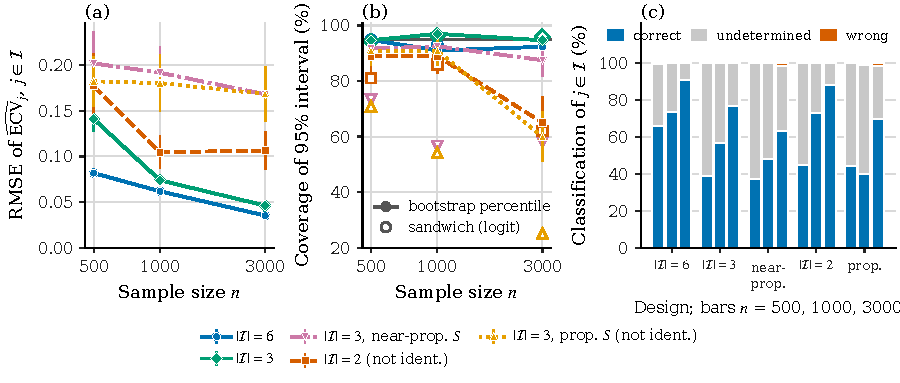
\includegraphics[width=6.0in]{figures/fig-sim-recovery.pdf}
\caption{X1, recovery of the item-level ECV and of the boundary set $\mathcal B_{0.5}$ (synthetic data). (a) RMSE of $\widehat{\mathrm{ECV}}_j$, pooled over the Israel-related items ($\pm2$ MCSE bars). (b) Coverage of nominal 95\% intervals: percentile bootstrap with $B=100$ (filled markers) and Wald intervals on the logit scale with sandwich standard errors (open markers, ``Wald (sandwich)''). (c) Classification of each Israel-related item from its bootstrap interval, against the true boundary set; bars are $n=500$, $1{,}000$ and $3{,}000$. The designs in grey are not identified ($|\mathcal I|=2$ and proportional $S$; \cref{thm:ident}(b),(c)) or only weakly identified (near-proportional $S$). Their ``correct'' shares, up to $88\%$, describe where the optimiser stops, not information in the data.}
\label{fig:sim-recovery}
\end{figure}

\paragraph{Non-identified and weakly identified designs}
With $|\mathcal I|=2$ the diagnostic is below $0.01$ in every replication, and the five starts reach the same objective value, within a relative $10^{-6}$, at points whose ECVs differ by $0.19$ to $0.22$ on average. The reported estimate is whichever point wins on rounding error, so its ``correct'' classifications carry no information from the data: both identified sets contain $\tau$, and bootstrap coverage falls from $89\%$ to $65\%$ as $n$ grows. In the proportional design sampling noise tilts the flat population objective, all starts reach the same point and the optimiser reports convergence in $92.5$ to $97.5\%$ of replications, yet the ECVs are not identified. The diagnostic is small (median $0.028$, $0.027$ and $0.0013$, against $0.061$ to $0.101$ in the identified designs), $35$ to $47.5\%$ of fits put a slope at its bound, the RMSE stays near $0.17$ to $0.18$, and Wald coverage falls from $71\%$ to $25\%$. The near-proportional design degrades continuously, as \cref{rem:id-heterogeneity} predicts. Its starts agree, but the median diagnostic is $0.012$ to $0.016$, its RMSE is $0.202$, $0.192$ and $0.168$ (against $0.141$, $0.074$ and $0.046$ for the identified design with the same Israel-related items), Wald coverage is $57$ to $73\%$ and $1.7\%$ of items are misclassified at $n=3{,}000$. The estimates wander along the near-flat curve from sample to sample, not from start to start. Agreement across starts therefore exposed the two-item case but neither the proportional nor the near-proportional case; the identification diagnostic flagged all three. The correlated-factors $\hat\rho_{SI}$ is recovered against its pseudo-true value ($0.589$ to $0.621$) in every design, including the non-identified ones (RMSE $0.016$ to $0.060$, coverage $90$ to $97.5\%$), so a precise $\hat\rho_{SI}$ says nothing about the boundary (\cref{thm:ident}(d)).

\paragraph{Testing heterogeneity (X9)}
Rule D2(ii) asks the data whether \cref{asm:id-het} holds before any ECV is reported. By \cref{lem:app-tetrad,lem:app-classes}, the assumption fails in a domain $\mathcal D$ exactly when every polychoric tetrad among its items vanishes. Its failure is therefore the null hypothesis of a single \emph{joint test}, the Wald test of a non-redundant set of $|\mathcal D|(|\mathcal D|-3)/2$ tetrads (35 for the stereotype domain, 77 for the Israel-related one; \cref{app:sim-est}). X9 compares it with the \emph{intersection--union test}, which accepts heterogeneity only if the joint test of $\mathcal D\setminus\{k\}$ rejects for every $k\in\mathcal D$, and with the \emph{earlier rule}, one of the $3{,}633$ within-domain tetrads significant after a Bonferroni adjustment (\cref{tab:sim-tetrad}). At $n=6{,}000$ the joint test has size $5.0$ to $6.5\%$ in each domain under both null configurations, the rule built on it (either domain, each at $2.5\%$) rejects in $5.2$ to $5.8\%$, and it rejects in every replication in the heterogeneous and two-lines configurations. At $n=1{,}500$ it over-rejects in the Israel-related domain ($11.0$ and $14.5\%$), so at smaller samples it should be calibrated by simulation. The intersection--union test is valid but very conservative (size at most $2.5\%$), because all its component hypotheses are true whenever \cref{asm:id-het} fails. It also tests a stronger property, heterogeneity that survives the removal of any one item: when heterogeneity rests on two items on a second line, it rejects in only $3.0$ and $3.5\%$ of replications at $n=6{,}000$, against $100\%$ for the joint test. The earlier rule is not powerless at the registered sizes ($100\%$ in the heterogeneous and two-lines configurations at $n=6{,}000$), but in the stereotype domain at $n=1{,}500$ its power is $52.0\%$ against $82.5\%$ for the joint test. No test detects the near-proportional configuration (rejection rates $6.2$ to $8.0\%$ at $n=6{,}000$); there the guard is the diagnostic of rule D2(iii).

\begin{table}[tbp]
\centering
\caption{X9, tests of within-domain heterogeneity (\cref{asm:id-het}) at the registered sizes (synthetic data; $R=400$ at $n=6{,}000$, $200$ at $n=1{,}500$). Rejection rates (\%) per domain at the 5\% level of the joint tetrad test, the intersection--union test (IUT) and the earlier Bonferroni rule over $3{,}633$ tetrads; D2(ii): heterogeneity accepted in at least one domain, with the joint and intersection--union tests at $2.5\%$ per domain. $^{0}$\Cref{asm:id-het} fails in both domains, so the rates are sizes. Two lines: two items of each domain lie on a second line through the origin of the loading plane.}
\label{tab:sim-tetrad}
\footnotesize
\setlength{\tabcolsep}{3.6pt}
% Generated by code/make_figures.py from results/sim_results.json -- do not edit by hand.
% X9: rejection rates (%) of tests of within-domain heterogeneity; R = {'6000': 400, '1500': 200}. Joint: Wald test of a
% non-redundant set of |D|(|D|-3)/2 tetrads at 5%; IUT: intersection-union test (joint test of every D minus
% one item rejects at 5%); Earlier: any of the 3633 within-domain tetrads, Bonferroni at 5%. D2(ii) columns: joint and IUT at 2.5% per domain; earlier rule as stated.
% superscript 0: configurations in which id-het fails (null); rejection rates there are sizes.
\begin{tabular}{@{}lrrrrrrrrrr@{}}
\toprule
 & & \multicolumn{3}{c}{Stereotype domain ($|\mathcal S|=10$)} & \multicolumn{3}{c}{Israel domain ($|\mathcal I|=14$)} & \multicolumn{3}{c}{D2(ii): either domain} \\
\cmidrule(lr){3-5} \cmidrule(lr){6-8} \cmidrule(lr){9-11}
Configuration & $n$ & Joint & IUT & Earlier & Joint & IUT & Earlier & Joint & IUT & Earlier \\
\midrule
Proportional$^{0}$ & 1500 & 9.0 & 0.5 & 0.5 & 11.0 & 1.0 & 4.0 & 13.0 & 0.0 & 4.5 \\
 & 6000 & 5.0 & 0.0 & 0.8 & 6.0 & 0.2 & 4.2 & 5.8 & 0.2 & 5.0 \\
\addlinespace
All but one proportional$^{0}$ & 1500 & 8.0 & 0.0 & 0.0 & 14.5 & 2.5 & 2.0 & 12.5 & 1.5 & 2.0 \\
 & 6000 & 5.5 & 0.0 & 0.5 & 6.5 & 1.0 & 4.8 & 5.2 & 0.5 & 5.0 \\
\addlinespace
Two lines & 1500 & 69.5 & 4.5 & 68.5 & 54.0 & 2.5 & 70.0 & 75.0 & 4.0 & 92.5 \\
 & 6000 & 100.0 & 3.0 & 100.0 & 100.0 & 3.5 & 100.0 & 100.0 & 3.2 & 100.0 \\
\addlinespace
Near-proportional & 1500 & 12.0 & 0.0 & 2.0 & 14.0 & 1.5 & 5.0 & 13.0 & 0.5 & 7.0 \\
 & 6000 & 8.0 & 0.2 & 1.0 & 6.2 & 0.5 & 4.0 & 7.0 & 0.0 & 5.0 \\
\addlinespace
Heterogeneous & 1500 & 82.5 & 30.0 & 52.0 & 100.0 & 99.5 & 100.0 & 100.0 & 100.0 & 100.0 \\
 & 6000 & 100.0 & 100.0 & 100.0 & 100.0 & 100.0 & 100.0 & 100.0 & 100.0 & 100.0 \\
\bottomrule
\end{tabular}

\end{table}

\subsection{Differential item functioning and anchors (X2, X2b, X7)}\label{sec:sim-dif}

X2 uses the six-item design in a reference and a focal group of $1{,}500$ each, with focal latent means $(\mu_G,\mu_S,\mu_I)=(0.3,0,0.3)$. In the focal group, I1 and I2 have uniform DIF, with thresholds lowered by $\kappa$ standard deviations of the latent response, and I3 has non-uniform DIF, with its general slope multiplied by $1-1.25\kappa$; its focal ECV falls from $0.40$ to $0.273$, $0.143$ and $0.040$ at $\kappa=0.2$, $0.4$ and $0.6$. \emph{Ignore DIF} fits the invariant model to both groups (\cref{rem:id-concurrent}); the \emph{oracle} frees exactly the DIF items; the \emph{anchored} fits hold an anchor set invariant and free all other items, with the correct set S1--S4, I5, I6 or one or two contaminated anchors (I1 for I5; I1, I2 for I5, I6). The \emph{drafted screen} adds a Wald test of equal slopes and thresholds for each non-anchor item, Benjamini--Hochberg at $q=0.05$, a flag only if the expected item scores also differ by at least $0.25$ at the focal mean of $G$, and a refit with flagged items free. The \emph{revised screen} of the plan (\cref{sec:design-groups}) drops the effect-size requirement; X7 runs it end to end on the same 400 data sets. \emph{Stereotype-only anchors} use S1--S4 and fix the focal $\mu_I$ and $\sigma^2_I$ (\cref{rem:id-anchor-S}). \Cref{tab:sim-dif} gives the results at $\kappa=0.4$; \cref{fig:sim-dif,tab:sim-difrev} in \cref{app:sim-tables} give them across $\kappa$.

\begin{table}[tbp]
\centering
\caption{X2 and X7, group comparisons under DIF at $\kappa=0.4$ (synthetic data; $1{,}500$ per group; $R=100$, the same data sets in every row). Bias, RMSE and coverage (\%, sandwich 95\% interval) of the focal-minus-reference latent mean differences, and bias of the reference and focal ECV of I3, the item with non-uniform DIF (true values $0.40$ and $0.143$). Drafted screen: Benjamini--Hochberg and an expected-score difference of at least $0.25$ (X2); revised screen: Benjamini--Hochberg alone, the rule of the plan (X7).}
\label{tab:sim-dif}
\footnotesize
\setlength{\tabcolsep}{4.0pt}
% Generated by code/make_figures.py from results/sim_results.json -- do not edit by hand.
% E2 at kappa = 0.4; n = 1500 per group; R = 100. Cov.: sandwich 95% interval.
% ECV_I3: the non-uniform-DIF item, true ECV 0.40 (reference) and 0.143 (focal).
\begin{tabular}{@{}lrrrrrrrr@{}}
\toprule
 & \multicolumn{3}{c}{$\mu_G^{(1)}-\mu_G^{(0)}=0.3$} & \multicolumn{3}{c}{$\mu_I^{(1)}-\mu_I^{(0)}=0.3$} & \multicolumn{2}{c}{$\mathrm{ECV}_{I3}$ bias} \\
\cmidrule(lr){2-4} \cmidrule(lr){5-7} \cmidrule(lr){8-9}
Strategy & Bias & RMSE & Cov. & Bias & RMSE & Cov. & Ref. & Focal \\
\midrule
Ignore DIF (full invariance) & +0.036 & 0.074 & 82 & +0.243 & 0.255 & 3 & $-$0.072 & +0.199 \\
Oracle (true DIF items free) & $-$0.006 & 0.047 & 98 & +0.008 & 0.062 & 95 & +0.009 & $-$0.002 \\
Correct anchors, free baseline & $-$0.008 & 0.049 & 100 & +0.010 & 0.065 & 95 & +0.010 & $-$0.002 \\
Correct anchors, tested + refit & +0.007 & 0.046 & 98 & $-$0.032 & 0.064 & 94 & $-$0.109 & +0.146 \\
1 contaminated anchor & $-$0.170 & 0.179 & 22 & +0.744 & 0.751 & 0 & +0.047 & +0.014 \\
1 contaminated, tested + refit & $-$0.117 & 0.129 & 48 & +0.688 & 0.696 & 0 & +0.058 & +0.021 \\
2 contaminated anchors & +0.149 & 0.191 & 54 & +0.669 & 0.682 & 0 & +0.003 & $-$0.005 \\
2 contaminated, tested + refit & +0.054 & 0.101 & 82 & +0.753 & 0.760 & 0 & $-$0.008 & $-$0.010 \\
Stereotype-only anchors (S1-S4) & $-$0.011 & 0.069 & 97 & \multicolumn{3}{c}{not identified} & +0.014 & $-$0.003 \\
\bottomrule
\end{tabular}

\end{table}

\paragraph{Ignoring DIF and anchors}
DIF confined to the Israel-related items is absorbed mainly by $\mu_I$, whose bias is $+0.098$, $+0.243$ and $+0.756$ at the three non-zero values of $\kappa$. It leaks into $\mu_G$ much less ($+0.029$, $+0.036$, $-0.001$), consistent with \cref{thm:dif-bias}(d)(ii). The ECVs move more: the focal ECV of I3 is overstated by $0.091$, $0.199$ and $0.381$, and at $\kappa=0.4$ the focal ECVs of the DIF-free items I4, I5 and I6 move by $+0.055$, $+0.044$ and $+0.030$, as \cref{thm:dif-bias}(d)(iii) predicts. With the correct anchors, and for the oracle, the bias of both mean differences and of both ECVs of I3 is at most $0.010$ in absolute value, and coverage is $92$ to $100\%$. One contaminated anchor biases $\hat\mu_G$ by $-0.093$, $-0.170$ and $-0.222$, with coverage falling to $3\%$; two bias it by $+0.083$, $+0.149$ and $+0.227$. The error does not stay with the faulty anchor (\cref{prop:anchor}): the screen flags DIF-free items at rates of $29.8\%$ and $42.9\%$ at $\kappa=0.4$, against $0.0\%$ with the correct anchors. The leave-one-anchor-out range of $\hat\mu_G$ is $0.043$ with the correct anchors and $0.133$ and $0.099$ with one and two contaminated ones. Stereotype-only anchors give $\hat\mu_G$ with bias between $-0.011$ and $0.000$ and coverage $94$ to $97\%$, at the cost of a larger RMSE ($0.069$ to $0.082$, against $0.049$ to $0.061$). In X2 that protection holds by construction, because only Israel-related items have DIF; X2b removes that feature.

\paragraph{The DIF screen, drafted and revised (X7)}
With the correct anchors the drafted screen never flags a DIF-free item, but it flags I3 in $0\%$, $0\%$ and $1\%$ of replications at $\kappa=0.2$, $0.4$ and $0.6$: a change in the general slope alone barely moves the expected score at the focal mean. It then treats I3 as invariant and reproduces the bias it is meant to prevent: at $\kappa=0.4$ the ECV of I3 is biased by $-0.109$ in the reference group and $+0.146$ in the focal group. We therefore revised the plan so that the multiplicity-adjusted test alone decides which items are freed, and re-simulated the revised screen end to end (X7). Its flags coincide with the Benjamini--Hochberg flags of X2 in every replication. With the correct anchors it frees I1 and I2 in $94$ and $98\%$ of replications at $\kappa=0.2$ and in $100\%$ at $\kappa\ge0.4$, and I3 in $41\%$, $100\%$ and $100\%$. It flags DIF-free items at mean rates of $0.7\%$, $3.6\%$, $2.8\%$ and $1.6\%$ at $\kappa=0$, $0.2$, $0.4$ and $0.6$, which costs precision but not bias. Downstream, $\hat\mu_G$ has bias between $-0.006$ and $0.000$ and coverage $95$ to $98\%$ at every $\kappa$, and the focal ECV of I3 is biased by $+0.042$, $-0.002$ and $+0.002$, against $+0.082$, $+0.146$ and $+0.190$ for the drafted screen. The remaining bias at $\kappa=0.2$ comes from the $59\%$ of replications in which I3 is not flagged ($+0.077$ there): small non-uniform DIF stays hard to detect with $1{,}500$ per group. With contaminated anchors the revised screen does not help ($\hat\mu_G$ biased by $-0.123$ and $+0.070$ at $\kappa=0.4$); only the choice of anchors addresses that.

\paragraph{DIF on the stereotype anchors (X2b)}
X2b gives two of the four stereotype anchors, S1 and S2, uniform DIF of $\kappa_S\in\{0.1,0.2,0.3\}$ in the same direction, with or without the Israel-related DIF of X2 at $\kappa_I=0.4$ (\cref{tab:sim-anchors}). At $\kappa_S=0.1$ the mean bias of $\hat\mu_G$ is $+0.025$ and $+0.031$ with the default anchors S1--S4, I5, I6 (coverage $96$ and $89\%$) and $+0.073$ and $+0.080$ with stereotype-only anchors (coverage $84$ and $75\%$). At $\kappa_S=0.2$ it is $+0.047$ and $+0.069$ against $+0.259$ and $+0.410$ (probability limits of the latter $+0.254$ and $+0.266$), and at $\kappa_S=0.3$ the stereotype-only fit breaks down (probability limits $+2.521$ and $+2.634$) while $21$ to $22\%$ of the default fits fail to converge. Stereotype-only anchoring is therefore not a safe default. It drops the assumption that Israel-related anchors are invariant at the price of resting everything on four stereotype items, and the same DIF on those items biases $\hat\mu_G$ two to three times as much as with the six default anchors (to first order, $+0.058$ against $+0.026$ per $0.1$ of $\kappa_S$), and more than linearly as $\kappa_S$ grows. The contamination leaves traces: at $\kappa_S=0.1$ and $\kappa_I=0$ the leave-one-anchor-out range of $\hat\mu_G$ is $0.165$ (default) and $0.464$ (stereotype-only), against $0.043$ with clean anchors, and the revised screen flags DIF-free stereotype items in up to $11\%$ of replications ($57\%$ at $\kappa_S=0.2$), which also reduces the bias of the default-anchor comparison to $+0.006$ and $+0.013$. The bound \eqref{eq:id-anchor-bound}, evaluated for this estimator at a stated maximum DIF $\delta$ on every anchor (\cref{app:sim-est}), is valid but wide. At $\delta=0.1$ the largest first-order bias of $\hat\mu_G$ is $0.345$ with the default anchors and $0.442$ with stereotype-only anchors, more than the true difference of $0.3$, and the norm bound is $0.707$ and $0.763$; at $\delta=0.2$, the value the plan registers, all of these double. The worst case has anchor DIF of opposite signs on anchors with different ECVs, which the model reads as a shift of $G$ against $S$; if all anchors' DIF has the same sign, the first-order bias of $\hat\mu_G$ is $0.104$ and $0.099$ at $\delta=0.1$. The pattern of X2b lies well inside the bound ($+0.026$ and $+0.058$ to first order at $\kappa_S=0.1$), but for stereotype-only anchors the probability limit exceeds the first-order value from $\kappa_S=0.2$ on, so the linear bound is not conservative there.

\subsection{Cross-loadings and acquiescence (X6)}\label{sec:sim-misspec}

X6 adds two misspecifications at the registered sizes, with 8 ID items with ECVs from $0.10$ to $0.70$ and 6 trope-based IT items with ECVs from $0.35$ to $0.85$ (\cref{app:sim-config}). In (a) every IT item also loads on $S$ with standardised loading $c\in\{0.1,0.2,0.3\}$. In (b) an acquiescence factor adds a slope $+\alpha$ to every positively worded item and $-\alpha$ to every reverse-keyed item, $\alpha\in\{0.25,0.40,0.55\}$ (standardised loadings $0.16$ to $0.36$), with the registered keying (four reverse-keyed items, two in S and two in ID, none in IT) or balanced keying (half of every block). The true values are the content ECVs of each item's own domain. Besides the standard bifactor fit we evaluate five remedies: a model with free loadings of all IT items on $S$; a method factor with one free slope and the instrument's keying, the random-intercept model of \citet{maydeuolivares2006}; a refit with $\mathcal I$ the ID items alone; the two-stage rule that the plan registers (\cref{sec:design-decisions}), which tests the mean residual correlation between IT and S items and, if the test rejects, uses the model with cross-loadings; and a one-item check proposed in an earlier draft, which tests the 60 residual correlations between IT and S items and fits a cross-loading for each IT item in turn. \Cref{fig:sim-misspec} shows the main results and \cref{tab:sim-misspec} gives them in full. Without misspecification no estimator has a bias above $0.006$ and all cover in $94$ to $95\%$ of cases.

\begin{figure}[tbp]
\centering
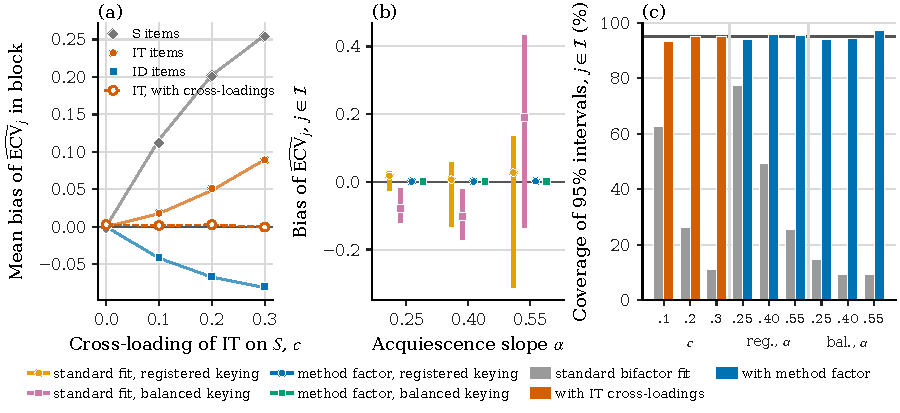
\includegraphics[width=6.0in]{figures/fig-sim-misspec.pdf}
\caption{X6, two misspecifications at the registered sizes (synthetic data; 10 S, 8 ID and 6 IT items; $n=6{,}000$; $R=100$ per cell). (a) Cross-loading of the IT items on $S$ with standardised loading $c$: mean bias of $\widehat{\mathrm{ECV}}_j$ by block in the standard bifactor fit (filled markers; lines are probability limits) and for the IT items in the model with cross-loadings (open markers). (b) Acquiescence with slope $\alpha$ and the registered (4 reverse-keyed items) or balanced keying: range (bar) and mean (marker) over the 14 Israel-related items of the bias of $\widehat{\mathrm{ECV}}_j$, in the standard fit and with a one-parameter method factor. (c) Coverage of the 95\% Wald intervals for the Israel-related ECVs in the standard fit (grey) and with the remedy for each misspecification: cross-loadings in the first three cells, the method factor in the others.}
\label{fig:sim-misspec}
\end{figure}

\paragraph{Cross-loading}
The standard fit credits the covariance between IT and S items to $G$. The ECVs of the IT items rise by $0.018$, $0.051$ and $0.089$ on average at $c=0.1$, $0.2$ and $0.3$, most for those with low ECV (IT1, true $0.35$, by $0.141$ at $c=0.3$), and IT3 (true $0.45$) is classified in $\mathcal B_{0.5}$ in $78\%$ of replications at $c=0.3$. The shift is not all towards ``in''. The whole general factor tilts towards $S$: the stereotype ECVs rise by $0.11$ to $0.25$ and the ID ECVs fall by $0.041$ to $0.080$ on average (ID8, true $0.70$, by $0.141$). Coverage of the intervals for the Israel-related ECVs falls to $63$, $26$ and $11\%$. The model with cross-loadings removes the bias (no item above $0.007$; coverage $93$ to $95\%$); the ID-only refit gives unbiased ID ECVs but none for the IT items; the method factor does nothing here. The plan's two-stage rule inherits the accuracy of the cross-loading model: the mean-residual test rejects in $100$, $100$ and $85\%$ of replications at $c=0.1$, $0.2$ and $0.3$ and in $5\%$ without cross-loadings, and the bias of every Israel-related ECV is at most $0.005$, $0.007$ and $0.021$. The one-item check flags at least one IT item in every replication with $c\ge0.1$, almost always through a one-item cross-loading, and under its rule the share of IT items on the wrong side of $\tau$ at $c=0.3$ falls from $14.2\%$ to $1.5\%$ (IT3 classified in: from $78\%$ to $9\%$). It achieves this by declaring items undetermined ($48.5\%$ of the IT items), not by correcting them: a cross-loading fitted for one item at a time leaves those of the others in place, so the one-item model still overstates the general-factor share of IT3 by $0.083$. Without misspecification it flags at least one IT item in $26\%$ of replications ($19.8$ against $19.0\%$ of IT items undetermined). The plan therefore fits the cross-loadings of the whole IT block.

\paragraph{Acquiescence}
With the registered keying, acquiescence acts like a second, nearly uniform general factor. The standard fit inflates the ECVs of positively worded Israel-related items with low ECV, by up to $0.030$, $0.057$ and $0.135$ at the three values of $\alpha$, and deflates those of the two reverse-keyed ID items, by up to $0.026$, $0.132$ and $0.312$. Block means move by at most $0.05$ and items rarely cross $\tau$ (at most $0.6\%$ wrongly classified), but coverage falls to $77$, $49$ and $26\%$. Balanced keying does not rescue the standard fit: it lowers every Israel-related ECV (block means $-0.064$ to $-0.128$ at $\alpha\le0.40$) and raises the stereotype ECVs by $0.14$ to $0.15$, and at $\alpha=0.55$ the fit breaks down, with $45\%$ of the Israel-related items on the wrong side of $\tau$. The one-parameter method factor removes the bias under both keyings (no item above $0.006$; coverage $94$ to $97\%$; its slope is estimated without bias). Without acquiescence it costs little ($10.7$ against $10.5\%$ of Israel-related items undetermined), and when the acquiescence slopes vary between items by a factor of three, which one slope cannot represent, it still reduces the largest bias from $0.112$ to $0.043$. The one-item check reacts to acquiescence too (an IT item flagged in $42$, $98$ and $100\%$ of replications with the registered keying) but cannot correct it, and the ID-only refit does not help. One caveat concerns rule D2(iii). The method slope enters the correlations only through its square, so its information vanishes without acquiescence and the diagnostic of the method-factor model is then zero. Computed over the content parameters it is $0.082$ to $0.105$ (median by cell), close to the $0.090$ of the standard fit without misspecification, so the plan, whose primary model includes the method factor, applies the rule to the content parameters.

\subsection{List experiments (X3, X8)}\label{sec:sim-list}

X3 simulates one sensitive item under the threshold-shift model of \cref{def:le-shift}, with standardised loading $0.6$ on $G$, $\pi=0.30$ and $\pi^D=0.20$, so $\SDB=0.10$ and monotonicity holds; a second scenario adds false endorsement $\pi^F=0.02$. Control items have prevalence $1/2$ and come in independent pairs with within-pair correlation $\rho$, and $n=3{,}000$ (\cref{fig:sim-list,tab:sim-list,tab:sim-listchoice} in \cref{app:sim-tables}). In the split design the estimator \eqref{eq:le-split} is unbiased in every cell, its Monte Carlo SD matches the exact formula to within $0.0008$, and its coverage is $94.3$ to $95.5\%$. The Neyman allocation of \cref{thm:design}(a) reduces the SD from $0.0487$ to $0.0456$ with four independent controls, a pilot-based allocation attains almost all of the gain, and negatively correlated pairs ($\rho=-0.6$) reduce it further, to $0.0331$ (\cref{prop:list-var}(c)). In the paired design the optimal allocation leaves the direct-only arm empty; the post-stratified and combined estimators have SDs $0.0249$ and $0.0226$, against $0.0339$ for the split design. With false endorsement, $\widehat{\SDB}_{\mathrm{PS}}$ stays unbiased while the combined estimator, read as an estimator of $\SDB$, is biased by $+0.0206$, the false-endorsement rate, and covers in $85.3\%$ of replications (\cref{thm:joint-sdb}(d)). Across $J\in\{2,\dots,6\}$, $\rho\in\{0,-0.6\}$ and floor and ceiling probabilities $\phi_{\mathrm c}=\phi_{\mathrm f}\in\{0,0.5\}$, the simulated bias is within $0.0027$ of \eqref{eq:le-fcbias} in all 20 cells. With $J=2$ and $\rho=0$ the exposure $\Pr(W_i\in\{0,J\})$ is $0.5$ and the bias $-0.073$; negative correlation cuts them to $0.2$ and $-0.031$. With floor and ceiling effects the MSE-optimal list is $J=2$ for $n\le1{,}000$, $J=4$ for $3{,}000\le n\le10^5$ and $J=6$ for $n\ge3\times10^5$, always with $\rho=-0.6$, and at $n=3{,}000$ the simulated MSEs pick the same list as the theory (\cref{thm:design}(c),(d)). The simulation does not measure disclosure.

\paragraph{Identifying the threshold shift (X8)}
X8 links the list experiment to the measurement model as in \cref{prop:list-irt}(b). The two-group bifactor model is fitted to the direct arm, and the shift $\delta_j$ of the sensitive item (I4 of the six-item design) is the root of \eqref{eq:le-irt-root} in each group, with the group's latent law from the anchored model. Two groups of $3{,}000$ with latent means $\bm0$ and $(0.5,0,0.3)$ are each split equally into a direct arm and two list arms (\cref{tab:sim-delta}). With a common shift of $0.4$ latent-response standard deviations, $\hat\delta_j$ is unbiased (bias $+0.0004$ and $-0.0034$, MCSE $0.009$ and $0.006$), its SD is $0.153$ and $0.109$ in the two groups, its standard error is accurate ($0.149$ and $0.109$), and 95\% intervals cover in $94.3$ and $95.7\%$ of replications; the list experiment contributes $81$ to $84\%$ of the variance. The test of a common shift (\cref{prop:list-irt}(c), \cref{prop:list-irt-ext}(d)) rejects in $3.0\%$ of replications when the shift is common, in $58\%$ when it is $0.4$ in one group and $0.8$ in the other, and in $14\%$ when the private response has its slope halved (\cref{prop:list-irt-ext}(e)), in which case $\hat\delta_j$ in the second group is biased by $-0.149$. The identification of \cref{prop:list-irt}(b) works at this sample size, but a list experiment detects only large departures from a common uniform shift.

\subsection{Small-area estimation and count indices (X4, X5)}\label{sec:sim-mrp}

X4 draws a new synthetic population of 50 areas in each replication, with differential non-response, and each respondent contributes an unbiased score of $G$, so it does not test the joint measurement and latent-regression model that \cref{sec:smallarea} recommends (\cref{fig:sim-mrp,tab:sim-mrp}). MRP has RMSE $0.168$, $0.133$ and $0.105$ at $n=1{,}000$, $3{,}000$ and $6{,}000$, against $0.342$, $0.232$ and $0.177$ for the unweighted direct mean, which non-response also biases by about $-0.1$; at $n=3{,}000$ its RMSE is $0.204$ against $0.602$ in areas with fewer than five respondents, and its coverage is $92.0$ to $94.7\%$. The two-step shortcut of \cref{prop:eap} has slopes on the true area deviations of $0.637$, $0.704$ and $0.762$, each equal to the estimated shrinkage factor ($0.845$, $0.844$, $0.846$) times the MRP slope to within $0.001$, and coverage $84.0$ to $86.0\%$.

\label{sec:sim-index}X5 computes the index $P_g(q)=\Pr(U_{i+}\ge q\mid g)$ for the eight stereotype items exactly, for two groups that differ only in their mean of $G$, with each item's agreement threshold shifted in the second group by an independent normal amount with standard deviation $s$ (\cref{fig:sim-index,tab:sim-index}). Under invariance the sign of $P_1(q)-P_0(q)$ always agrees with $\Delta\mu_G$ (\cref{prop:index}(a)). With $s=0.1$ the sign is reversed in $20.1$ to $21.1\%$ of configurations when $|\Delta\mu_G|=0.05$ and never when $|\Delta\mu_G|\ge0.2$; with $s=0.3$, in $39.4$ to $41.3\%$ at $|\Delta\mu_G|=0.05$ and $4.2$ to $7.8\%$ at $0.3$. With $\Delta\mu_G=0.2$ and full invariance, a second group whose standard deviation of $G$ is $0.6$ has the lower index for every $q\ge4$ (\cref{prop:index}(b)), and random non-uniform DIF makes the sign depend on $q$ in $25.9$ to $63.6\%$ of configurations (\cref{prop:index-dif}(d)). This concerns synthetic items only.

\subsection{What the simulation does and does not show}\label{sec:sim-limits}

In the designs studied, the formal results describe finite-sample behaviour. Heterogeneity within a domain identifies the boundary estimands, which are recovered with small bias and close to nominal Wald coverage at $n\ge1{,}000$; two Israel-related items or proportional stereotype loadings leave them unidentified, and near-proportional loadings degrade them badly. Agreement across starts exposed the two-item case but neither the proportional nor the near-proportional case; the identification diagnostic flagged all three. A joint tetrad test detects heterogeneity at the registered sizes with close to nominal size, but no test separates near-proportional from proportional loadings. Ignored DIF and contaminated anchors bias comparisons as \cref{thm:dif-bias,prop:anchor} predict. Stereotype-only anchoring protects comparisons of $G$ against DIF on Israel-related items but is two to three times as sensitive as the default anchors to DIF on the stereotype anchors. The revised DIF screen, re-simulated end to end, removes the bias the drafted screen left. A cross-loading of trope-based items on $S$ and acquiescence both distort the boundary estimands, not always towards ``in'', and a cross-loading model and a one-parameter method factor remove the respective biases. The list-experiment formulas hold to Monte Carlo precision and a list experiment identifies the threshold shift; MRP improves on direct estimation in small areas; count indices misrank groups under modest DIF. The simulation changed the plan in several places: the DIF screen, simultaneous intervals for the boundary set, the identification rule, the misspecification checks and the anchor sensitivity analysis (\cref{sec:design}).

It does not show the following. (i) \emph{Full-information fits}: the full-information and Bayesian fits the plan reports as sensitivity analyses target the same parameters, but their finite-sample behaviour can differ, and the logistic link is not simulated (\cref{rem:id-logit}). (ii) \emph{Exact interval calibration}: the bootstrap with $B=100$ undercovers slightly in some cells. (iii) \emph{Estimates in non-identified designs}: there the point estimates are optimiser artefacts. (iv) \emph{General DIF}: X2, X2b and X7 have two groups of equal size and a few DIF patterns; the Mantel--Haenszel cross-check and alignment are not simulated, and the anchor bound is evaluated at first order and at population values. (v) \emph{Other misspecification}: X6 covers one cross-loading pattern and acquiescence; local dependence, other response styles, non-normal latent distributions and correlated specific factors are not simulated (\cref{sec:discussion}). (vi) \emph{Violated list-experiment assumptions}: X3 and X8 have no design effects and no liars (\cref{asm:le}), and do not measure disclosure. (vii) \emph{The joint latent MRP model}: X4 starts from an unbiased score of $G$. Above all, the simulation contains no information about real attitudes. Its parameters were chosen to test the methods; they are not estimates of anything and are not calibrated to any survey.
}{}
\IfFileExists{sections/08-design.tex}{\section{A pre-registered survey design and analysis plan}\label{sec:design}

This section is the design and analysis plan that we will register, time-stamped and with the commit hash of the analysis code, before any respondent is interviewed \citep{nosek2018}. It fixes in advance the item bank structure, the groups for invariance testing, the list-experiment module, the sample and poststratification frame, the estimands, the threshold $\tau$, the decision rules and the model checks. Any departure will be reported as a deviation, with its reason. The estimators are those of \cref{sec:model,sec:identification,sec:sensitive,sec:smallarea}, implemented and tested on synthetic data in \cref{sec:simulation}. No survey has been fielded. The items described below are \emph{constructs and selection criteria}, not a validated instrument. Item wording will be developed through the pre-testing steps of \cref{sec:design-items} and registered only once it is final.

\subsection{Population, constructs and model}\label{sec:design-constructs}

The target population is the adult household population of one country. The plan is written for the United States because the poststratification frame of \cref{sec:design-sampling} is available there; \cref{sec:design-groups} describes the cross-national extension. The measurement model is the bifactor graded response model of \cref{sec:model}, with a general factor $G$ and specific factors $S$ (classic stereotypes) and $I$ (Israel-related attitudes) \citep{samejima1969,gibbons1992,reise2012}. Responses are on a five-point agreement scale, so $C_j=4$ for every attitude item. The primary model adds an acquiescence factor \citep{maydeuolivares2006}: a person-level tendency to agree, orthogonal to $G$, $S$ and $I$, with one loading common to all attitude items, entered with a positive sign for agree-keyed items and a negative sign for reverse-keyed items, which are scored in the direction of their construct. $\mathrm{ECV}_j$ is computed from the content loadings as in \cref{def:boundary}. The identification results of \cref{sec:identification} are stated without this factor; its effect on recovery was checked by simulation. Without such a factor, acquiescence loads on $G$ and moves the boundary estimands (\cref{sec:model-meaning}); in the simulation the factor removed that bias, whereas balancing the keying without it did not (\cref{sec:design-decisions}). The correlated-factors model, with factors $S$ and $I$ and no general factor, and a unidimensional model are fitted alongside it as pre-registered comparison models.

\subsection{Item bank}\label{sec:design-items}

\Cref{tab:design-items} lists the item blocks. Every block is described by construct; none of the content descriptions below is a questionnaire item.

\begin{table}[tb]
\centering
\caption{Item bank structure. Counts are targets for the main survey; the pilot fields about 1.5 times as many candidates per block. $\mathcal{S}$, $\mathcal{I}$ and $\mathcal{A}$ are the item sets of \cref{sec:model}.}\label{tab:design-items}
\footnotesize
\setlength{\tabcolsep}{4pt}
\renewcommand{\arraystretch}{1.15}
\begin{tabularx}{\textwidth}{@{}>{\raggedright\arraybackslash}p{2.6cm}>{\raggedright\arraybackslash}p{1.9cm}c>{\raggedright\arraybackslash}X@{}}
\toprule
Block & Model role & Items & Construct and content (generic) \\
\midrule
S: classic stereotypes & $\mathcal{S}$; loads on $G$ and $S$ & 10 & Statements attributing to Jews as a group excessive power or influence (economic, political, media), disloyalty, conspiratorial intent, or responsibility for historical misfortunes; statements that minimise or deny the Holocaust. Content categories follow those used in prior batteries (\cref{sec:bg-surveys}) without reusing their wording. \\
\addlinespace
ID: Israel, disputed categories & $\mathcal{I}$; loads on $G$ and $I$ & 8 & Statements in the categories of Israel-related speech on which the definitions of \cref{sec:bg-definitions} disagree: positions on specific policies or actions of Israeli governments and of the Israeli state, on Zionism, on boycotts, and on comparisons with other historical cases. Selected to span those categories. \\
\addlinespace
IT: Israel, classic tropes & $\mathcal{I}$; loads on $G$ and $I$ & 6 & Israel-related statements that invoke classic antisemitic tropes, for example claims of secret control by Israel or its supporters, or collective responsibility of Jews for Israel's conduct. Selected from categories that more than one definition treats as antisemitic. \\
\addlinespace
A: anchors & $\mathcal{A}\subset\mathcal{S}\cup\mathcal{I}$ & 6 & Items expected, on substantive grounds and pilot evidence, to function equivalently across the groups of \cref{tab:design-groups}: four from S and two from the Israel-related blocks, so that every factor has anchors. Counted within their own blocks. \\
\addlinespace
C: comparison states & auxiliary & 16 & For each ID item, parallel statements about a comparable policy or case of each of two pre-registered comparison states. Not in the measurement model. \\
\addlinespace
R: reverse-keyed & $\mathcal{S}\cup\mathcal{I}$ & 4 & Favourably worded items, two in S and two in ID, which separate the acquiescence factor of the primary model from content (\cref{sec:design-constructs}). Counted within their own blocks. \\
\addlinespace
Q: data quality & auxiliary & 3 & Instructed-response attention checks, placed in separate blocks. \\
\addlinespace
K: knowledge and covariates & auxiliary & -- & Factual knowledge of the Israeli--Palestinian conflict and of other conflicts; ideology; religiosity and affiliation; birth year; region; demographics for poststratification. \\
\bottomrule
\end{tabularx}
\end{table}

\paragraph{Selection criteria}
Candidate items enter the pilot only if they meet five criteria.
\begin{enumerate}[(i)]
  \item \emph{One construct per item.} Each attitude item is written to load on $G$ and on exactly one specific factor. Double-barrelled statements (for example, a statement about a policy combined with a trope) are excluded, because they would make the item-level estimand of \cref{def:boundary} uninterpretable.
  \item \emph{Coverage of the disputed categories.} The ID block includes at least one item for each category of Israel-related speech on which \cref{sec:bg-definitions} records disagreement. The IT block draws on categories that more than one definition treats as antisemitic. Neither block is chosen to make the boundary set larger or smaller.
  \item \emph{Definitional tags, recorded but not used in estimation.} Before fielding, each Israel-related item is tagged with how the text of each definition treats its content category, or ``unclear''. Tags are assigned independently by advisory-group members who hold different views of the definitions (\cref{sec:ethics}), and disagreements are recorded rather than resolved. Tags are metadata. They let readers relate the estimated boundary set to any definition, but no estimand depends on them.
  \item \emph{Pre-testing.} Cognitive interviews with respondents who differ in ideology, age and religious background check that each item is understood as intended. Items that are understood differently by different groups are revised or dropped before the pilot; this is the cheapest stage at which to remove DIF.
  \item \emph{Identification.} \Cref{thm:ident} needs at least four items in one domain whose general-factor shares are not all equal save one, and the joint tetrad test of rule D2(ii) in \cref{sec:design-decisions} needs no more (its intersection--union diagnostic needs five). Both domains exceed these counts, with room to drop items at the pilot stage. The pilot also checks the loading conditions of \cref{thm:ident}, including heterogeneity of general-factor shares within a domain (\cref{asm:id-het}). A block whose specific-factor loadings are near zero in the pilot, or whose items have nearly equal general-factor shares, is redesigned before the main survey; the simulation shows that near-proportional loadings make the boundary estimands unreliable at realistic sample sizes (\cref{sec:sim-recovery}).
\end{enumerate}
\paragraph{Pilot}
A pilot sample, which is not used in any confirmatory analysis, screens candidates. Items are dropped for severe floor or ceiling effects, for high item non-response, or for DIF flagged in the pilot by both screening methods of \cref{sec:design-groups}. The pilot also supplies the variance inputs for \cref{thm:design}. The final item set, the anchor set $\mathcal{A}$ and all thresholds are frozen in the registration after the pilot and before the main fieldwork.

\paragraph{Administration}
The questionnaire is self-administered online, which tends to elicit more reporting of sensitive information than interviewer administration \citep{kreuter2008}. The list-experiment module (\cref{sec:design-list}) comes first, before any direct question about Jews or Israel. The order of the S and Israel-related blocks is randomised, and items are randomised within blocks. Block order is recorded and treated as a grouping variable for the invariance checks, so that priming between the two domains can be detected.

\subsection{Groups for invariance testing}\label{sec:design-groups}

\Cref{tab:design-groups} lists the pre-registered groupings. Each is tested separately; intersections are not tested, because their cells are too small.

\begin{table}[tbp]
\centering
\caption{Pre-registered groupings for invariance and DIF testing. Groups with fewer than $n_{\min}=300$ respondents are merged with an adjacent group or omitted, as fixed in the registration.}\label{tab:design-groups}
\footnotesize
\renewcommand{\arraystretch}{1.15}
\begin{tabularx}{\textwidth}{@{}l>{\raggedright\arraybackslash}X>{\raggedright\arraybackslash}X@{}}
\toprule
Grouping & Categories & Rationale \\
\midrule
Ideology & Self-placement, collapsed to left / centre / right & Political identity may shape responses to Israel-related items, and to some stereotype items, independently of $G$ (\cref{sec:bg-invariance}) \\
Cohort & Ages 18--29, 30--44, 45--64, 65+ & Generational differences in the salience and framing of both domains \\
Religiosity & Attendance at religious services: never; less than monthly; monthly or more & Religious commitments may affect both domains \\
Region & Four census regions & Required for the small-area model (\cref{sec:design-sampling}) \\
Block order & S first / Israel-related first & Detects priming between domains \\
Country (extension) & Countries in a cross-national replication & Translation and context; anchoring vignettes considered \citep{king2004} \\
\bottomrule
\end{tabularx}
\end{table}

For each grouping the procedure is fixed.
\begin{enumerate}[1.]
  \item Fit the configural multiple-group bifactor model, then constrain loadings (metric) and then thresholds (scalar) \citep{meredith1993,millsap2011}. Changes in fit are reported with the caveats of \citet{chen2007}; they do not by themselves decide invariance.
  \item Screen every item for DIF with two methods: Wald tests of equal slopes and thresholds in the multiple-group fit of the primary estimator, with the anchor set held invariant, the limited-information counterpart of the likelihood-ratio tests of \citet{thissen1993} and the test used in the simulation (\cref{sec:sim-dif}); and the Mantel--Haenszel procedure with the total score on the remaining items as the matching variable \citep{holland1988}. Multiplicity is controlled by the Benjamini--Hochberg procedure at a false discovery rate of 0.05 within each grouping \citep{benjamini1995}. An item is flagged if its Wald test is significant after this adjustment. The Mantel--Haenszel procedure, which is sensitive mainly to uniform DIF, is a cross-check, and disagreements between the two methods are reported. The size of each flagged item's DIF is a secondary screen. We report the difference in expected item score between the group-specific and the reference item parameters, averaged in absolute value over the group's latent distribution, and describe flagged items with a difference below 0.25 scale points as having small DIF; they are freed all the same. An earlier draft flagged an item only if it was also at least 0.25 scale points apart at the group's mean of $G$. In the simulation that requirement almost never flagged an item with non-uniform DIF, whose expected scores differ little near the group mean, and the procedure then reproduced the bias it was meant to remove (\cref{sec:sim-dif}). The revised screen was re-simulated end to end on the same data sets (\cref{sec:simulation}). With the correct anchors it freed the item with non-uniform DIF in $41\%$ of replications at the smallest DIF and in every replication at larger DIF; that item's focal ECV was then biased by $+0.042$ at the smallest DIF and by at most $0.002$ in absolute value at larger DIF, and the bias of the difference in means of $G$ was at most $0.006$ in absolute value.
  \item Fit the partial-invariance model with flagged items freed and the anchors constrained \citep{byrne1989}. Group comparisons of latent means and of $\mathrm{ECV}_j$ are reported from this model. Their identification rests on \cref{prop:anchor}. Comparisons of $G$ and of the group-specific ECVs are also reported, for every grouping, from a model anchored in the four stereotype anchors alone (\cref{rem:id-anchor-S}). That model need not assume that any Israel-related item functions identically across groups; it assumes that the stereotype anchors do, which is testable only in part (\cref{prop:anchor}(b)). It is a sensitivity analysis, not the primary comparison. Resting on four anchors instead of six, it is more exposed to DIF on them: in the simulation, DIF of $0.1$ on two stereotype anchors biased its difference in means of $G$ by $+0.073$ and $+0.080$, against $+0.025$ and $+0.031$ with the default anchors, and at $0.3$ it broke down (\cref{sec:sim-dif}). Every anchored comparison of latent means is therefore reported with the bound \eqref{eq:id-anchor-bound}, evaluated at the estimated information and maximised over all uniform anchor DIF of at most $\delta=0.2$ standard deviations of each anchor's latent response, the smallest Israel-item DIF in the simulation (\cref{sec:sim-dif}); the bound at $0.4$ is reported alongside. The bound is wide. In the simulated design, at $\delta=0.2$ it allows a first-order bias of the difference in means of $G$ of up to $0.69$ with the default anchors and $0.89$ with stereotype-only anchors, against a true difference of $0.3$; if all anchors' DIF has the same sign, the largest bias is about $0.2$ for both. As a further check on the anchors, each anchor is in turn freed and the comparisons recomputed; the spread of these leave-one-anchor-out estimates is reported.
  \item As a sensitivity analysis, refit with the alignment method \citep{asparouhov2014}, which does not require a pre-selected anchor set.
\end{enumerate}
Items flagged for non-uniform DIF have group-specific loadings, so their $\mathrm{ECV}_j$ is reported by group (\cref{sec:design-estimands}). \Cref{thm:dif-bias} gives the bias that the analysis would incur if it ignored flagged DIF; we report that bias, evaluated at the estimates, as a diagnostic.

\subsection{The list-experiment module}\label{sec:design-list}

\paragraph{Sensitive items}
The module covers four sensitive items drawn from the final item bank: two from S and two from the Israel-related blocks (one ID, one IT). For each sensitive item $j$, every respondent is randomised independently to one of the three arms of \cref{sec:sensitive}: \emph{direct} ($\mathsf{D}$), in which item $j$ appears in the direct battery; \emph{list control} ($\mathsf{C}$); or \emph{list treatment} ($\mathsf{T}$). Respondents in the two list arms are not asked item $j$ directly in the main questionnaire. For them, item $j$ is missing by design, and since assignment is random the missingness is ignorable in the measurement model. The prevalence $\pi_j$ targeted by the list is agreement with item $j$, coded as the top two categories of the five-point scale. The direct-arm counterpart is $\pi^D_j$, and $\mathrm{SDB}_j=\pi_j-\pi^D_j$ as in \cref{sec:sensitive}.

\paragraph{Control lists}
Each sensitive item has its own list of $J$ control items ($J$ as in \cref{sec:sensitive}). $J$ and the arm probabilities $(r_D,r_C,r_T)$ are chosen by \cref{thm:design}, with $J\in\{3,4,5\}$ and the inputs (control-item prevalences and their covariance) estimated in the pilot. Control items are low in sensitivity and unrelated to Jews or Israel. Following \citet{glynn2013}, each list includes negatively correlated pairs of control items. This reduces the variance of the count and makes it rare for a respondent to agree with all or none of the control items, which limits ceiling and floor effects. It can also make the count more informative about the sensitive answer (\cref{sec:sens-design}), so every list must meet two registered disclosure bounds, evaluated at the pilot estimates of the control-count distribution and of the sensitive item's prevalence: the mutual information $I(Y_i;Z_i\mid\mathsf{T})$ between the treatment count and the sensitive answer is at most $0.15$ bits, and at most $15\%$ of treated respondents have posterior $\Pr(Z_i=1\mid Y_i,\mathsf{T})\ge0.5$. For comparison, four independent control items of prevalence $1/2$ with $\pi=0.2$ give $0.11$ bits and $11\%$, and two pairs with within-pair correlation $-0.6$ give $0.24$ bits and $30\%$. Within the lists that meet both bounds, $J$ and the correlation are chosen by \cref{thm:design}(d); a list that fails either bound is replaced before the main survey.

\paragraph{Checks}
For each list we report the test of \citet{blair2012} for design effects. The decision rule is in \cref{sec:design-decisions}. We also estimate the floor-and-ceiling model of \citet{blair2012}, and report the multivariate estimator of \citet{imai2011} with the covariates of \cref{tab:design-groups}. In addition, a random 20\% of list-arm respondents are asked item $j$ directly at the very end of the questionnaire. This supports the combined estimator and placebo tests of \citet{aronow2015} as a secondary analysis. It does not enter the primary estimator, because a direct answer given after the list may be affected by it. For these respondents the file records the direct answer as well as the count, so the list gives them no additional protection; \cref{sec:ethics-data} sets out how these records are handled.

\paragraph{The cost of the module}
\Cref{prop:list-var} gives the variance of the difference-in-means estimator. As illustrative arithmetic, not a result, suppose that both count variances equal $1$ ($\sigma_{\mathsf{C}}^2=\sigma_{\mathsf{T}}^2=1$), that $\pi^D_j=0.2$, and that the three arms are of equal size $m$; these are the inputs used for \cref{thm:design}(a) in \cref{app:pd-design}. Equal count variances assume that the control items covary slightly negatively with the sensitive item. With four independent control items of prevalence $1/2$ and $\pi_j=0.2$, $\sigma_{\mathsf{T}}^2=1.16$ instead (\cref{sec:sens-var}). Under the first assumption the variance of $\widehat{\mathrm{SDB}}_j$ is about $(2+0.16)/m$, and detecting $\mathrm{SDB}_j=0.10$ with power 0.8 in a two-sided test at the 5\% level requires $m\approx 1{,}700$, or about 5,100 respondents in total for that item. With $\sigma_{\mathsf{T}}^2=1.16$ it requires $m\approx1{,}820$. Detecting $\mathrm{SDB}_j=0.05$ requires four times as many, about 20{,}000 respondents for each item, against a planned 6{,}000. A meta-analysis of list experiments found sensitivity biases typically below ten percentage points \citep{blair2020}, so the module is not powered for the effects that are most plausible. $\mathrm{SDB}_j$ is therefore a secondary estimand (E5 in \cref{sec:design-estimands}), with a registered precision target instead of a power target: at the planned sample size and the allocation of \cref{thm:design}, the 95\% interval for each $\mathrm{SDB}_j$ should have a half-width of at most $0.07$ (about $0.06$ under the inputs above). Two features of the design reduce the cost. Each respondent serves in some arm for every sensitive item, so the four experiments share one sample. And the joint model of \cref{thm:joint-sdb} borrows strength across items and from the measurement model. Equal allocation is not optimal; \cref{thm:design} gives the allocation actually used.

\subsection{Sampling, weighting and poststratification}\label{sec:design-sampling}

\paragraph{Primary sample}
The primary sample is drawn from a probability-based online panel recruited by address-based sampling, with a target of 6,000 completed interviews. The target will be revised in the registration from the power analysis of \cref{sec:design-power}. Design weights are raked to population margins for age, sex, education, race and ethnicity, and region. These weights are used for the national estimands.

\paragraph{Optional opt-in supplement}
For small-area estimation, a non-probability (opt-in) supplement may be added in under-sampled areas. Opt-in samples can be less accurate than probability samples, even after demographic weighting, and their accuracy varies widely across surveys and measures \citep{yeager2011,baker2013}. Model-based adjustment can nonetheless make them informative \citep{wang2015}. The supplement therefore enters only the MRP model. It carries an indicator for sample source, and its estimates are compared with those from the probability sample in areas where both are available. If the two disagree by more than the pre-registered tolerance (twice the combined standard error of an area mean of $G$), the supplement is dropped.

\paragraph{Poststratification}
The small-area estimand is the poststratified mean in \cref{eq:mrp} \citep{gelman1997,park2004}. Cells $k$ are formed by state $\times$ age (4) $\times$ sex (2) $\times$ education (4) $\times$ race and ethnicity (4). Population counts $N_k$ come from the most recent five-year American Community Survey tables available at registration. Ideology and religiosity are not in census tables. For estimates that condition on them, the cell table is extended with a joint distribution estimated from a large reference survey, and the uncertainty of that extension is propagated. State-level predictors are fixed at registration. Multilevel regression with poststratification performs well relative to disaggregation of national samples, especially when state samples are small \citep{lax2009}. Its limits are those of the model: the estimates depend on the predictors, and design-based and model-based weighting can diverge \citep{gelman2007}. We therefore report a design-based estimate alongside every MRP estimate for areas large enough to have one.

\paragraph{Campus module (optional)}
Campus-level estimates require a separate frame of students. If such a module is fielded, its poststrata are institution type $\times$ enrolment characteristics, with counts from institutional enrolment data. Estimates for named institutions will not be published (\cref{sec:ethics}).

\subsection{Pre-registered estimands}\label{sec:design-estimands}

\paragraph{Primary estimands}
\begin{enumerate}[(E1)]
  \item For every Israel-related item $j\in\mathcal{I}$, the item-level explained common variance $\mathrm{ECV}_j$ of \cref{def:boundary}, with a 95\% interval.
  \item The boundary set $\mathcal{B}_\tau=\{j\in\mathcal{I}:\mathrm{ECV}_j\ge\tau\}$ with $\tau=0.5$, the point at which the general factor accounts for at least half of an item's common variance. The value of $\tau$ is fixed here, before any data are seen. Each item is classified three ways from simultaneous 95\% intervals for all $\mathrm{ECV}_j$, $j\in\mathcal{I}$: Bonferroni-adjusted Wald intervals on the logit scale (\cref{prop:id-boundary-test}(b)). An item is \emph{in} $\mathcal{B}_\tau$ if its lower limit is at least $\tau$, \emph{out} if its upper limit is below $\tau$, and \emph{undetermined} otherwise. With simultaneous intervals, the items classified in and the items not classified out bracket $\mathcal{B}_\tau$ with probability at least 0.95 in large samples, which pointwise intervals do not guarantee; in the simulation they did so in every replication with six Israel-related items (\cref{sec:sim-recovery}). Undetermined is a reportable outcome, not a failure.
  \item The latent correlation between the stereotype factor and the Israel-attitude factor in the correlated-factors model, with a 95\% interval.
  \item Differences in the latent mean of $G$ between the groups of \cref{tab:design-groups}, under the partial-invariance model, with stereotype-only anchoring as a sensitivity analysis (\cref{sec:design-groups}).
\end{enumerate}

\paragraph{Secondary estimands}
\begin{enumerate}[(E1)]\setcounter{enumi}{4}
  \item For each sensitive item $j$, $\mathrm{SDB}_j$ from the joint model of \cref{thm:joint-sdb}, with the precision target of \cref{sec:design-list}.
  \item $\mathrm{ECV}_j$ and $\mathcal{B}_\tau$ by group, with the same simultaneous rule, for groupings in which loadings are not invariant.
  \item MRP estimates of the mean of $G$ by state and census region (\cref{eq:mrp}); boundary estimands are estimated by region only, as a multiple-group model.
  \item Within-person contrasts between each ID item and its comparison-state counterparts (block C), as a description of whether the same kind of statement is endorsed differently about Israel and about other states. A contrast is not by itself evidence of a double standard: respondents may know more about one case, so contrasts are also reported conditional on the knowledge measures of block K \citep{beattie2017}.
  \item The proportion agreeing with at least $q$ of the $M$ S items (\cref{sec:sa-index}), computed for comparability with published indices, and reported by group only together with the invariance diagnostics that \cref{prop:index} shows to be necessary.
\end{enumerate}
\paragraph{Sensitivity analyses}
$\mathcal{B}_\tau$ is also reported for $\tau\in\{0.3,0.7\}$; these do not change the primary classification. Other sensitivity analyses: exclusion of respondents who fail two or more attention checks (the primary analysis keeps them, because passing attention checks correlates with respondent characteristics; \citealp{berinsky2014}); a refit in which $\mathcal I$ is the ID block alone, which removes the trope-based items most exposed to a cross-loading on $S$; the primary model without the acquiescence factor; group comparisons anchored in the stereotype items alone, with the bound \eqref{eq:id-anchor-bound} (\cref{sec:design-groups}); the alignment model; the bifactor-$(S-1)$ model of \citet{eid2017}, in which the general factor is defined by the stereotype items alone (\cref{rem:id-s1}); percentile-bootstrap intervals with at least 1{,}000 resamples, as a check on the Wald intervals of E1 and E2; full-information and Bayesian fits (\cref{sec:design-decisions}); and Schmid--Leiman and exploratory bifactor solutions \citep{schmid1957,reise2012}.

\subsection{Model checks and decision rules}\label{sec:design-decisions}

\paragraph{Estimation and checks}
The primary estimator is the two-step limited-information estimator validated in the simulation (\cref{sec:sim-design}): thresholds and polychoric correlations \citep{olsson1979}, with an asymptotic covariance matrix from per-respondent influence functions, then weighted least squares with diagonal weights and sandwich standard errors, from a default start and at least 20 random starts. It is primary because it is the estimator whose recovery, coverage and identification diagnostic the simulation established; the diagnostic of rule D2(iii) and the power study of \cref{sec:design-power} are defined for it. Full-information marginal maximum likelihood, exploiting the dimension reduction of the bifactor structure \citep{gibbons1992}, and a Bayesian fit with weakly informative priors \citep{gelman2013} are reported as sensitivity analyses. Under the normal-ogive model all three target the same parameters (\cref{lem:id-reduction}), so a material disagreement between them is itself reported as a finding about the fit. Model adequacy is assessed with limited-information fit statistics, residual correlations between item pairs, and, for the Bayesian fit, posterior predictive checks of item-pair and sum-score distributions. The bifactor indices of \citet{rodriguez2016} are reported for all three models: explained common variance, $\omega_H$, percentage of uncontaminated correlations and construct replicability. Their thresholds are descriptive and do not enter the decision rules.

\paragraph{Cross-loadings and response style}
Two misspecifications would move the ECVs of Israel-related items, though not all in the same direction: a loading of trope-based items on the stereotype factor, which a bifactor model without that loading credits to $G$, and acquiescence (\cref{sec:model-meaning}). In the simulation (\cref{sec:sim-misspec}), a cross-loading of $0.3$ raised the mean ECV of the IT items by $0.089$ and lowered that of the ID items by $0.080$, and with the registered keying acquiescence moved the ECVs of single Israel-related items by between $+0.135$ and $-0.312$, upwards for agree-keyed and downwards for reverse-keyed items. Acquiescence is modelled in the primary model (\cref{sec:design-constructs}). In the simulation of both misspecifications at the registered item counts and $n=6{,}000$, the acquiescence factor kept the bias of every Israel-related ECV below $0.007$ under both the registered and a balanced keying, against biases of up to $0.43$ without it; balancing the keying without the factor did not remove the bias. With acquiescence slopes that differ between items, which the factor does not model, the largest bias was $0.043$, against $0.112$ without it. For cross-loadings, the mean residual polychoric correlation between the IT and the S items under the primary fit is tested one-sided at the 5\% level. If the test rejects, the ECVs and classifications of the Israel-related items are taken from a model in which every IT item also loads on $S$, with the cross-loadings of the whole IT block fitted jointly, $\mathrm{ECV}_j$ still computed from the loadings on $G$ and $I$, and the estimated cross-loadings reported. In the simulation, with the test computed from the bifactor fit, it rejected in $85$ to $100\%$ of replications when the IT items cross-loaded on $S$ with standardised loadings of $0.1$ to $0.3$ (in $5\%$ without cross-loadings), and this two-stage rule kept the bias of every Israel-related ECV below $0.021$, against biases of up to $0.141$ for the bifactor model alone. A check that fits a cross-loading for one IT item at a time, which an earlier draft proposed, is not used: at $c=0.3$ it cut the share of IT items on the wrong side of $\tau$ from $14.2\%$ to $1.5\%$ only by leaving $48.5\%$ of them undetermined, and its one-item fits stayed biased, because the other IT items' cross-loadings remain unmodelled (\cref{sec:sim-misspec}). The refit with $\mathcal I$ restricted to the ID block (\cref{sec:design-estimands}) is the corresponding check that does not rely on the test.

\paragraph{Decision rules}
The following rules are fixed in advance.
\begin{description}[style=unboxed,leftmargin=0pt]
  \item[D1, structure.] If the bifactor model fails the pre-registered fit criteria and the correlated-factors model passes them, we report E3 and no boundary set. If both fail, we report descriptive item statistics and the model comparison only.
  \item[D2, identification.] Item-level ECVs and the boundary set are reported only if the data support the conditions of \cref{thm:ident}. (i) Each domain has at least three items whose specific loadings have 95\% intervals that exclude zero (\cref{asm:id-spec}). (ii) In at least one domain $\mathcal D$ the items are heterogeneous in the sense of \cref{asm:id-het}. By \cref{lem:app-tetrad,lem:app-classes}, the assumption fails in $\mathcal D$ exactly when every polychoric tetrad $R_{k_1k_2}R_{k_3k_4}-R_{k_1k_3}R_{k_2k_4}$ among its items vanishes (under the bifactor model each equals $D_{k_1k_4}D_{k_2k_3}$). Its failure is therefore the null hypothesis of a single test, the simultaneous Wald test of a non-redundant set of $|\mathcal D|(|\mathcal D|-3)/2$ tetrads of $\mathcal D$ \citep{bollen1993tetrad}. It uses only the polychoric correlations and their asymptotic covariance, so it is regular whether or not the bifactor model is identified, and it replaces the Bonferroni rule over all quadruples of an earlier draft. Each domain is tested at the 2.5\% level, so that the rule, which needs heterogeneity in only one domain, has level at most 5\%. At $n=6{,}000$ and the registered item counts the simulation found sizes close to nominal and power of one in the heterogeneous designs (\cref{sec:simulation}); at a smaller sample size the critical values are calibrated by simulation, because the test over-rejects at $n=1{,}500$ in the larger domain. The joint test needs only four items in $\mathcal D$, which give two non-redundant tetrads. We also report the intersection--union version \citep{berger1982}, which accepts heterogeneity only if the same test rejects for $\mathcal D\setminus\{k\}$ for every $k\in\mathcal D$, and so needs five items. The null hypothesis for $\mathcal D\setminus\{k\}$, that all its tetrads vanish, says that all its items but at most one lie on one line, not that its loadings are proportional. The intersection--union version therefore tests a stronger property, heterogeneity that survives the removal of any one item, and is conservative; it is a robustness diagnostic and does not decide. Neither test detects near-proportional loadings, against which (iii) is the guard. (iii) The fit is numerically identified: the identification diagnostic of \cref{sec:sim-recovery}, the ratio of the smallest to the largest singular value of the weighted Jacobian of the fitted polychoric correlations of the primary fit with respect to its content loadings (on $G$, $S$ and $I$), exceeds a cut-off fixed in the registration from the simulation of \cref{sec:design-power}, and at least 20 random starts reach the same optimum with no loading at a bound. The slope of the acquiescence factor is left out of the diagnostic because it enters the correlations only through its square: without acquiescence its information vanishes and the diagnostic over all parameters is zero, whereas over the content loadings it was $0.082$ to $0.105$ in the simulation, close to the value for the model without the factor (\cref{sec:sim-misspec}). If (i) or (ii) fails, every $\mathrm{ECV}_j$ is reported as not identified, no boundary set is reported, and E3 is reported instead; if only two Israel-related items carry specific variance, the identified sets of \cref{thm:ident}(c) are reported. If only (iii) fails, the ECVs are reported as weakly identified and every item is classified as undetermined. The interval-based classification of E2 is used only when (iii) holds, because the guarantees of \cref{prop:id-boundary-test} are pointwise and unreliable near the non-identified set (\cref{rem:id-test-uniform}). Agreement across starts is necessary, not sufficient: in the simulation it exposed the two-item case but neither the proportional nor the near-proportional case (\cref{sec:sim-recovery}).
  \item[D3, invariance.] Group comparisons (E4, E6) are reported only for groupings in which the anchors that pass the DIF screen satisfy the rank condition of \cref{prop:anchor}(a). There must be at least two such anchors in each domain, at least one with a non-zero specific loading in each domain, and, within at least one domain, two anchors whose loading vectors are not proportional, judged by a 95\% interval for their determinant $D_{kl}$ \eqref{eq:id-det} that excludes zero. Two proportional anchors per domain do not suffice. If no Israel-related anchor passes but the stereotype anchors contain a non-proportional pair, comparisons of $G$ and of the group-specific ECVs are reported, labelled as resting on the stereotype anchors alone, and comparisons of the Israel-attitude mean are not (\cref{rem:id-anchor-S}). Otherwise only within-group estimates and the alignment results are reported, labelled exploratory (\cref{prop:anchor}). Whatever the outcome, the stereotype-anchored comparisons and the bound \eqref{eq:id-anchor-bound} of step~3 in \cref{sec:design-groups} are reported alongside.
  \item[D4, design effects.] If the design-effect test rejects at the 5\% level for a list, that list's estimate is not used to correct the direct estimate; E5 for that item is reported as not estimable. If floor or ceiling effects are detected, the floor-and-ceiling model of \citet{blair2012} replaces the difference in means.
  \item[D5, completeness.] Every primary estimand is reported for every item and group, whatever its direction or magnitude. Items are dropped after fielding only for the pre-registered quality reasons (item non-response above 10\% or failed comprehension in the pilot), and dropped items are listed.
\end{description}

\subsection{Power and precision}\label{sec:design-power}

The sample size is set by Monte Carlo simulation, a practical approach to power analysis for latent-variable models of this size \citep{muthen2002}. We use the simulation code of \cref{sec:simulation}, which implements the primary estimator, with item parameters set from the pilot. The registration will report three precision targets: the half-width of the 95\% interval for each $\mathrm{ECV}_j$ at the national level; the power to detect DIF with an expected-score difference of 0.25 scale points in the smallest group of \cref{tab:design-groups}; and the half-width of the 95\% interval for each $\mathrm{SDB}_j$ under the allocation of \cref{thm:design} (target $0.07$; \cref{sec:design-list}). The same simulation fixes the cut-off of the identification diagnostic in rule D2(iii) and reports the power of the joint tetrad test of rule D2(ii), and of its intersection--union version, at the pilot parameters. The recovery results of \cref{sec:simulation} indicate which of these binds. If the budget cannot meet all three, the list module is reduced (fewer sensitive items) before the main sample is, because E1--E4 do not depend on it.

\subsection{Replication package and transparency}\label{sec:design-replication}

The following will be released. The registration document, with the commit hash of the analysis code. The code for every estimator, the simulation study and the figures. The final item bank, including wording, block, definitional tags and the record of tag disagreements, released after fieldwork closes. Aggregate results for every estimand, and the poststratification table. A log of deviations from the plan. De-identified microdata will be deposited with a data archive under restricted access, because the data combine religion, political opinion and geography (\cref{sec:ethics}). Synthetic microdata generated from the fitted model will be released openly, so that the code can be run without access to the restricted file.

\begin{table}[tbp]
\centering
\caption{Timeline, in months from the start of the project.}\label{tab:design-timeline}
\small
\begin{tabular}{@{}lll@{}}
\toprule
Months & Phase & Output \\
\midrule
1--2 & Advisory group convened; candidate items drafted; tagging & Candidate bank; tag record \\
3--4 & Cognitive interviews; ethics review & Revised bank; approval \\
5 & Pilot fieldwork and screening & Pilot report (not confirmatory) \\
6 & Item bank, anchors, $J$, allocation and thresholds frozen & Registration, with code hash \\
7--8 & Main fieldwork & Raw data, held by panel provider \\
9 & Data-quality checks; data freeze & Frozen analysis file \\
10--11 & Confirmatory analysis as registered & Results for E1--E9; deviations log \\
12 & Release & Paper, replication package, data deposit \\
\bottomrule
\end{tabular}
\end{table}

\Cref{tab:design-timeline} gives the timeline. Fieldwork dates will be recorded and reported with every estimate. Attitudes about Israel may move with events, so the estimates describe the population at the time of fieldwork and are not assumed to be stable.
}{}
\IfFileExists{sections/09-ethics.tex}{\section{Ethics and responsible interpretation}\label{sec:ethics}

The survey of \cref{sec:design} asks people to respond to statements about Jews and about Israel, some of which many readers will find offensive and some of which express positions held in good faith by large parts of the public. Its respondents include Jewish people, Israelis, Palestinians, Muslims and people of every political view. Its results will be read in a debate in which the stakes are high and the parties distrust each other's evidence. This section sets out the safeguards the plan commits to and the limits on what the results can be used to show.

\subsection{Review, consent and debriefing}\label{sec:ethics-consent}

The protocol will be reviewed by an institutional review board before the pilot, and again before the main survey if the pilot leads to changes. The consent page states, before any question is shown, that the survey includes statements about Jews and about Israel, that some of these statements are offensive stereotypes, that respondents may skip any question or stop at any time without penalty, and that answers are confidential. Consent is recorded before the first item.

Two features of the design need explicit justification to the review board. First, respondents are shown stereotype statements. These are needed to measure the attitudes they express, and the item bank uses the smallest number that identification and precision allow (\cref{sec:design-items}). Second, the list experiment does not tell respondents which item on a list is of interest. This is indirect questioning, not deception: nothing false is stated, and the purpose of the technique is explained in the debriefing.

Every respondent who starts the survey, including those who stop early, sees a debriefing page. It states that the statements about Jews were included because they are common stereotypes whose prevalence the study measures, and that their inclusion does not mean the researchers regard them as true. It states that the Israel-related statements span views held across the political spectrum and that their inclusion implies no judgement about them. It explains the list experiment, gives contact details for the research team and the review board, and lists sources of support for respondents who found the content distressing. The pilot measures whether respondents report distress, and the debriefing is revised if it is inadequate.

\subsection{Data protection}\label{sec:ethics-data}

The survey data combine religion, political opinion, attitudes toward an ethnic and religious group, and geography. In the European Union, data revealing political opinions or religious beliefs are special categories of personal data \citep{gdpr2016}; any cross-national extension will be designed under that regime, and we treat the US data with the same care. The research team does not receive names, addresses or contact details; these stay with the panel provider, and respondents are linked across waves only through a pseudonymous identifier. Geography is held at the level needed for the small-area model and no finer. The analysis file is stored encrypted, with access limited to named analysts. Microdata are released only under restricted access, and openly only in synthetic form (\cref{sec:design-replication}). Released tables apply small-cell suppression and are checked for disclosure by differencing against other released tables \citep{hundepool2012}. Small-area results are released only as model-based estimates with intervals.

\subsection{Population associations are not individual diagnoses}\label{sec:ethics-individual}

The estimands of this paper describe populations. Four consequences follow, and every output will state them.
\begin{itemize}
  \item A respondent's estimated position on $G$ is a model-based summary with substantial uncertainty. It is used only to estimate population quantities. No individual score will be reported, and the methods are not a screening tool for individuals.
  \item An item's membership of the boundary set $B_\tau$ means that, \emph{in the surveyed population}, most of the common variance in responses to it is shared with responses to classic stereotypes. It does not mean that a particular person who endorses the item holds hostile attitudes toward Jews, or that a particular utterance with similar content is antisemitic in its context. Conversely, an item outside $B_\tau$ is not thereby shown to be acceptable in every context. Definitions of antisemitism classify speech and conduct in context, often with reference to intent (\cref{sec:bg-definitions}); our estimands do not.
  \item Differences in mean $G$ between ideological, religious, age or regional groups are differences between averages of overlapping distributions. They will always be reported with intervals and alongside the within-group spread, never as rankings of groups. They say nothing about any member of a group.
  \item Small-area estimates describe areas, not the people in them, and model-based estimates for small areas lean on the model. Estimates for named campuses will not be published (\cref{sec:design-sampling}), because the risk of stigmatising a student body outweighs the value of the estimate.
\end{itemize}
These points apply to every group, including groups whose members are themselves frequent targets of prejudice. The analysis plan does not single out any religious or ethnic group for comparison; religiosity enters as a measure of practice, not of affiliation (\cref{tab:design-groups}).

\subsection{Misuse in political debate}\label{sec:ethics-misuse}

The results bear on a contested question, and any of them can be quoted selectively. An item placed in $B_\tau$ can be cited as proof that a category of criticism of Israel is antisemitic; an item placed outside it can be cited as proof that it never is. Neither reading is supported. We commit to the following.
\begin{itemize}
  \item \emph{Publication whatever the results.} Every pre-registered estimand will be published, whichever position in the definitional debate it appears to support and including indeterminate classifications and null results (decision rule D5).
  \item \emph{No adjudication.} No output will describe the results as validating or refuting the IHRA working definition, the Jerusalem Declaration or the Nexus Document. Results will be presented item by item, with the definitional tags of \cref{sec:design-items}, so that readers can relate them to any definition themselves.
  \item \emph{Full context in every release.} Releases will state the population, the fieldwork dates, the threshold $\tau$ and the uncertainty of every classification. Plain-language summaries will say what the results do not show.
  \item \emph{Correction.} Errors found after publication will be corrected publicly, in the paper and in the replication package.
\end{itemize}

\subsection{Advisory input}\label{sec:ethics-advisory}

Before items are drafted, we will convene an advisory group whose members hold different views on the definitions of \cref{sec:bg-definitions}. It will include representatives of Jewish communal organisations with differing positions on those definitions; Palestinian, Arab and Muslim community organisations; scholars who have argued for different definitions; civil-liberties and academic-freedom specialists; and survey methodologists. The group reviews the item bank for balance and wording, assigns the definitional tags independently, reviews the consent and debriefing texts, and comments on how results are communicated. It has no veto over the results, and its members are not asked to endorse them. Membership, funding sources and any relationship between the research team and organisations with a stake in the results will be disclosed in every output.

\subsection{Neutrality}\label{sec:ethics-neutrality}

The Kornstein Lab exists to study antisemitism. Readers are entitled to ask whether that mission shapes the instrument or the analysis. We do not ask readers to rely on our intentions. The design builds in four protections. The threshold $\tau$, the decision rules and the item bank are fixed before data collection (\cref{sec:design}). The item bank covers every disputed category of Israel-related speech, and its balance is reviewed by advisers with opposing views (\cref{sec:ethics-advisory}). The estimands are symmetric: the same quantity is computed for every item, and an item can fall in or out of $B_\tau$ under the same rule. And the code, the synthetic data and the registered plan are public (\cref{sec:design-replication}), so that anyone can check that the analysis follows the plan. The paper's aim is to make an empirical sub-question of the boundary debate answerable by evidence that people on every side can inspect, not to settle the debate.
}{}
\IfFileExists{sections/10-discussion.tex}{\section{Discussion}\label{sec:discussion}

\paragraph{What a boundary map could show}
The public argument about Israel-related speech is usually conducted as a
single question: is this kind of criticism antisemitic? The framework
replaces it with many narrower questions, one for each statement in a
pre-registered item bank, each with an answer that has an interval and
stated assumptions. For each Israel-related statement, a boundary map would
show how much of the common variance in responses to it is shared, through
the general factor, with responses to classic stereotypes
(\cref{def:boundary}), and whether that share lies clearly above, clearly
below or indeterminately around a threshold fixed in advance
(\cref{fig:boundary,prop:id-boundary-test}). It would show this only where the data identify it
(\cref{thm:ident}), and it would say so where they do not. The
correlated-factors model adds a coarser summary, the latent correlation of
the two attitude domains. It is the quantity closest to the scale-level
associations reported in earlier studies (\cref{sec:bg-prior}), and it
cannot by itself separate a common cause from correlated but distinct
attitudes (\cref{prop:model-sl}); the item-level map can, where the items
within a domain differ in their general-factor share.

Every outcome of such a map is informative to every side of the debate.
Someone who holds that a category of Israel-related speech typically
expresses hostility toward Jews learns whether, in the surveyed population,
statements in that category covary with classic stereotypes as that view
implies. Someone who holds that the category typically expresses a distinct
political attitude learns the same thing about the opposite claim. Both learn
where the evidence is indeterminate at the sample size used, which is itself
a finding. Under partial invariance the map can also be compared across
political, generational and national groups (\cref{thm:dif-bias,prop:anchor}).
These comparisons can be anchored in the stereotype items alone
(\cref{rem:id-anchor-S}), so no one need assume that any Israel-related
statement means the same thing to the groups being compared, an assumption
that would itself be contested.
An item could sit inside the boundary set in one group and outside it in
another. A finding of that kind would bear directly on whether one rule can
be applied to speakers from every group, a question that the definitions
answer differently through the weight they give to context
(\cref{sec:bg-definitions}). The list-experiment module would show whether
direct answers understate or overstate endorsement, item by item
(\cref{thm:joint-sdb}). Under a uniform threshold shift, social desirability
biases prevalences but leaves the boundary estimands unchanged
(\cref{prop:list-irt}); it affects latent-mean comparisons only if the shift
differs between groups, where it acts as DIF. The map is therefore robust to
the simplest form of strategic answering, though not to a shift that acts
differently on the general and the specific parts of an item's response. Multilevel regression and
poststratification would carry the latent trait to regions and states with
honest intervals (\cref{eq:mrp}), and \cref{prop:index} explains why a
stereotype-count index cannot do the same job without invariance
diagnostics.

\paragraph{What it could not show}
A boundary map is not a verdict. It does not say which speech ought to be
called antisemitic, and it is compatible with more than one answer. A
definition could reasonably treat a statement as antisemitic even if its
$\mathrm{ECV}_j$ is low, for example because of what the statement does to
the people it is about, or because definitions classify speech in context.
A definition could equally decline to treat a statement as antisemitic even
if its $\mathrm{ECV}_j$ is high, because covariance with stereotypes across
a population does not establish what any particular speaker meant.

Nor is the map a diagnosis of anyone. $\mathrm{ECV}_j$ is a ratio of
variances: it says how responses to an item move with the general factor
across the population, not how many of the item's endorsers stand high on
that factor (\cref{sec:model-meaning}). An item can have a high share and
still be endorsed by many respondents who stand low on the general factor,
if its threshold is low. Nor is the map causal. A general factor summarises shared variance, and shared variance can have
several sources: a common attitude, a common information environment, or a
common response style. The design separates some of these, through
knowledge measures, reverse-keyed items and comparison-state items
(\cref{sec:design-items}), but not all. Finally, the general factor means
only what its items make it mean. We read it as hostility toward Jews as
Jews because the stereotype items that define it are not themselves in
dispute between the definitions. If those items also share a broader
disposition, such as a general readiness to endorse conspiratorial claims,
the general factor absorbs it, and the boundary estimands inherit that
ambiguity. This is why the stereotype battery, and not only the
Israel-related items, is fixed before fieldwork and reviewed by advisers with
opposing views (\cref{sec:ethics-advisory}). Whether the general factor
should be defined as what both domains share, as in our primary model, or
anchored in the stereotype domain alone, as in the bifactor-$(S-1)$ variant
reported as a sensitivity analysis (\cref{rem:id-s1}), is itself part of the
substantive question.

\paragraph{Limitations}
We stress five.

\emph{Survey mode.} The plan uses a self-administered online panel
(\cref{sec:design-items}). Mode affects what respondents are willing to
report \citep{kreuter2008,tourangeau2007}, panels differ in coverage, and the
assumptions of the list experiment, no design effect and no liars
(\cref{asm:le}), can be tested only in part (\cref{cor:le-tests}). Estimates
from one mode need not transfer to another, and the social-desirability
correction is specific to the mode in which it is estimated.

\emph{Dependence on item wording.} $\mathrm{ECV}_j$ is a property of an item,
a particular wording answered by a particular population, and not of a
category of speech. Two wordings of the same idea can load differently, and a
statement that is double-barrelled, ambiguous or unfamiliar can land
anywhere. The map generalises from items to categories only as far as the
bank samples the wordings of each category, which is why the plan requires
several items per disputed category and records how each definition treats
each item (\cref{sec:design-items}). A claim about a category resting on one
item would be a claim about that item.

\emph{Translation across countries and cultures.} A statement about Israel
does not mean the same thing in every country, language or political
culture. Translation can create differential item functioning, and scalar
invariance is often hard to establish across countries
\citep{davidov2014,steenkamp1998}. A cross-national boundary map therefore
needs a translation protocol, invariance testing of every item in every
country, and, where invariance fails, anchoring vignettes \citep{king2004} or
alignment \citep{asparouhov2014}. Without these, a difference in boundary
sets between countries could reflect translation rather than attitudes.

\emph{Latent-variable assumptions.} Every result rests on a model: a graded
response link, local independence given the factors, normal latent
distributions, orthogonal factors in the bifactor model, and an assignment of
each item to exactly one specific factor. If an Israel-related item also
loads on the stereotype factor, a bifactor model without that cross-loading
will tend to credit the shared variance to the general factor. Our
identification results state what is identified under the model, not that
the model is true. The decision rules compare the bifactor model with the
correlated-factors and unidimensional models and report a boundary set only
when the bifactor model passes pre-registered fit criteria
(\cref{sec:design-decisions}). The simulation study tests the estimators
under the departures it simulates (\cref{sec:simulation}), not under every
departure that real data might present.

\emph{Population association is not individual intent.} The estimands
describe how attitudes covary across a population at the time of fieldwork.
They say nothing about the intentions of any respondent, speaker or
organisation, and they may change as events change what statements about
Israel mean to the people answering them. Every output will carry these
limits (\cref{sec:ethics-individual}).

\paragraph{Extensions}
Three extensions seem most valuable. First, \emph{longitudinal invariance}.
Attitudes about Israel may move with events, and so may the meaning of the
items. Tracking a boundary map over time requires invariance across waves as
well as groups, with anchor items that are themselves stable over time; an
item that drifts across the boundary could be changing in meaning, not in
the attitudes behind it. The event calendars of the second paper in this
series \citep{kornsteinlab2026contagion} offer a principled way to place
waves before and after salient external events. Second, \emph{conjoint
designs}. The item-level estimand is observational: it describes how
responses to fixed wordings covary. A conjoint design that randomises
attributes of a statement, such as whether it refers to Israel or to another
state, whether it invokes a classic trope, and how it is framed, would
estimate the average causal effect of each attribute on endorsement, the
average marginal component effect of \citet{hainmueller2014}. That would separate the content of a statement from
its wording, and so address the dependence on wording described above.
Third, \emph{linkage to text}. The lab's other projects propose to measure
antisemitism in online discourse, to evaluate detection algorithms and to
trace narratives \citep{kornsteinlab2026measurement,kornsteinlab2026detection,kornsteinlab2026narratives}.
A boundary map could inform them: the definitional tags and estimated
$\mathrm{ECV}_j$ of each item give annotators and classifiers a graded,
population-based description of Israel-related content in place of a single
binary label. In the other direction, narratives observed in text can
suggest wordings for the item bank. Any linkage of survey respondents to
their own online text would require separate consent and its own ethics
review (\cref{sec:ethics}).

\paragraph{Measurement as common ground}
The debate over where criticism of Israel ends and antisemitism begins will
not be settled by a survey. It turns on values, law and the experience of
people on every side, and those are not measured by covariance. But the
debate also contains empirical claims, and those can be tested in a way that
does not depend on which side one is on. The threshold, the items, the
decision rules and the code are fixed before the data are seen; the same
rule is applied to every item; and every estimate is published whatever its
direction. A result produced that way is not a weapon for either side. It is
a shared reference point that people who disagree about definitions can
inspect, criticise and replicate. That is what measurement can offer a
contested question: not an answer to it, but common ground on which to argue
about it.
}{}

\bibliographystyle{plainnat}
\bibliography{refs,bib/sources,bib/theory,bib/models,bib/lead}

\clearpage
\appendix
\IfFileExists{appendix/A-proofs-measurement.tex}{\section{Proofs for Sections~\ref{sec:model}--\ref{sec:identification}}\label{app:proofs-measurement}

Throughout, $\operatorname{offdiag}(\bm M)$ denotes the off-diagonal entries of a square matrix $\bm M$, and two matrices are \emph{off-diagonally equal} if their off-diagonal entries agree. For a domain $\mathcal D\in\{\mathcal S,\mathcal I\}$ we write $\bm w=\bm\lambda_{\mathcal DG}$ and $\bm s=\bm\lambda_{\mathcal Ds}$ for the standardised general and specific loadings of its items, and we drop the superscript $\mathcal D$ when the domain is clear. Response patterns take finitely many values, so every expectation below is a finite sum. All models considered are $C^\infty$ in their parameters, because $F$ is smooth and the latent distributions are Gaussian.

\subsection{Algebraic lemmas}\label{app:pm-lemmas}

\begin{lemma}[Rank-one factorisations]\label{lem:app-rank1}
If $\bm u\bm v^\top=\tilde{\bm u}\tilde{\bm v}^\top\neq\bm0$, then $\tilde{\bm u}=t\bm u$ and $\tilde{\bm v}=\bm v/t$ for a unique $t\neq0$.
\end{lemma}

\begin{proof}
Choose $k,l$ with $u_kv_l\neq0$; then $\tilde u_k\tilde v_l=u_kv_l\neq0$. For every $k'$, $\tilde u_{k'}=\tilde u_{k'}\tilde v_l/\tilde v_l=u_{k'}v_l/\tilde v_l$, so $\tilde{\bm u}=t\bm u$ with $t=v_l/\tilde v_l$. Likewise $\tilde{\bm v}=(u_k/\tilde u_k)\bm v=\bm v/t$. Uniqueness is clear because $\bm u\neq\bm0$.
\end{proof}

\begin{lemma}[One-factor off-diagonal structure]\label{lem:app-onefactor}
Let $\bm u\in\mathbb R^p$ have at least three non-zero entries. If $\tilde{\bm u}\tilde{\bm u}^\top$ and $\bm u\bm u^\top$ are off-diagonally equal, then $\tilde{\bm u}=\pm\bm u$.
\end{lemma}

\begin{proof}
Let $N=\{k:u_k\neq0\}$, so $|N|\ge3$. For $k\in N$ pick distinct $l,m\in N\setminus\{k\}$. Then $\tilde u_l\tilde u_m=u_lu_m\neq0$ and
$\tilde u_k^2=(\tilde u_k\tilde u_l)(\tilde u_k\tilde u_m)/(\tilde u_l\tilde u_m)=u_k^2$. For $k\notin N$ and any $l\in N$, $\tilde u_k\tilde u_l=0$ with $\tilde u_l\neq0$, so $\tilde u_k=0$. Finally, $\tilde u_k\tilde u_l=u_ku_l$ for $k,l\in N$ gives $\operatorname{sgn}(\tilde u_k/u_k)=\operatorname{sgn}(\tilde u_l/u_l)$, so the sign change is common to all entries.
\end{proof}

\begin{lemma}[Tetrads]\label{lem:app-tetrad}
For $\bm w,\bm s\in\mathbb R^p$, $\delta\in\mathbb R$ and $\bm M=\bm s\bm s^\top+\delta\bm w\bm w^\top$, define $D_{kl}=w_ks_l-s_kw_l$. For distinct $k_1,\dots,k_4$,
\[
  M_{k_1k_2}M_{k_3k_4}-M_{k_1k_3}M_{k_2k_4}=\delta\,D_{k_1k_4}D_{k_2k_3},
\]
whereas the same tetrad of any rank-one matrix $\bm u\bm u^\top$ vanishes.
\end{lemma}

\begin{proof}
Write $1,\dots,4$ for $k_1,\dots,k_4$. Expanding, the terms in $\delta^0$ ($s_1s_2s_3s_4$) and in $\delta^2$ ($w_1w_2w_3w_4$) cancel, leaving
$\delta\,(s_1s_2w_3w_4+w_1w_2s_3s_4-s_1s_3w_2w_4-w_1w_3s_2s_4)$. On the other hand,
$D_{14}D_{23}=(w_1s_4-s_1w_4)(w_2s_3-s_2w_3)=w_1w_2s_3s_4-w_1w_3s_2s_4-s_1s_3w_2w_4+s_1s_2w_3w_4$, which is the same bracket. For $\bm u\bm u^\top$ the tetrad is $u_1u_2u_3u_4-u_1u_3u_2u_4=0$.
\end{proof}

\begin{lemma}[When heterogeneity fails]\label{lem:app-classes}
Let a domain contain $p\ge4$ items whose loading vectors $(w_k,s_k)$ are all non-zero. There exist distinct $k_1,\dots,k_4$ with $D_{k_1k_4}D_{k_2k_3}\neq0$ if and only if it is not the case that all items, with at most one exception, lie on one line through the origin.
\end{lemma}

\begin{proof}
$D_{kl}=0$ if and only if the two non-zero vectors are proportional, which is an equivalence relation; call its classes \emph{lines}. Note that the condition concerns two disjoint non-proportional pairs, and relabelling within the quadruple is free. If one line contains all items but at most one, every pair of distinct items that avoids the exceptional item is proportional. Two disjoint pairs cannot both contain the exceptional item, so no quadruple works. Conversely, suppose no line contains $p-1$ items. If two lines each contain at least two items, say $k_1,k_2$ on one and $k_3,k_4$ on the other, the pairs $(k_1,k_3)$ and $(k_2,k_4)$ are non-proportional. Otherwise every line but at most one is a singleton, and since no line has $p-1\ge3$ items there are at least three lines. Pick $x,y,z$ on three different lines and a fourth item $u$. If $u$ is not on the line of $x$, the pairs $(x,u)$ and $(y,z)$ work; otherwise $(u,y)$ and $(x,z)$ do.
\end{proof}

\subsection{Proof of \texorpdfstring{\cref{lem:id-reduction}}{the reduction lemma}}\label{app:pm-reduction}

Under the normal-ogive link, \eqref{eq:model-lr} with $\varepsilon_j\sim\mathrm N(0,1)$ gives $\bm Y^*\sim\mathrm N_J(\bm A\bm\mu,\bm A\bm\Sigma\bm A^\top+\bm I_J)$, and $\bm Y$ is its discretisation at the thresholds. Let $Z_j=(Y^*_j-\bm a_j^\top\bm\mu)/s_j$. Then $\bm Z\sim\mathrm N_J(\bm0,\bm R)$ and $Y_j=\sum_c\ind{Z_j>\bar b_{jc}}$, so the law of $\bm Y$ depends on the parameters only through $(\bar{\bm b},\bm R)$. Conversely, $\Pr(Y_j\ge c)=\Phi(-\bar b_{jc})$ determines $\bar b_{jc}$. For $j\neq k$, $\Pr(Y_j\ge1,Y_k\ge1)=\Phi_2(-\bar b_{j1},-\bar b_{k1};R_{jk})$, where $\Phi_2(\cdot,\cdot;\rho)$ is the standard bivariate normal distribution function with correlation $\rho$. Since $\partial\Phi_2(x,y;\rho)/\partial\rho=\phi_2(x,y;\rho)>0$ for $|\rho|<1$ \citep{plackett1954}, and $|R_{jk}|<1$ because the error variances are positive, this probability determines $R_{jk}$. In the reference group, $s_j^2=1+\|\bm a_j\|^2$ and $h_j^2=\|\bm a_j\|^2/(1+\|\bm a_j\|^2)$, so $s_j^{-2}=1-h_j^2$, $R_{jk}=\bm a_j^\top\bm a_k/(s_js_k)=\bm\lambda_j^\top\bm\lambda_k$ and $\bar b_{jc}=b_{jc}(1-h_j^2)^{1/2}$. Given $\bm\lambda_j$ with $\|\bm\lambda_j\|^2<1$, the map $\bm a_j=\bm\lambda_j(1-\|\bm\lambda_j\|^2)^{-1/2}$ satisfies $1+\|\bm a_j\|^2=(1-\|\bm\lambda_j\|^2)^{-1}$ and hence returns $\bm\lambda_j$. This establishes the bijection and its inverse. \qed

\subsection{Proof of \texorpdfstring{\cref{thm:ident}}{the identification theorem}}\label{app:pm-ident}

By \cref{lem:id-reduction}, two reference-group parameter values are observationally equivalent if and only if they share $\bar{\bm b}$ and $\operatorname{offdiag}(\bm\Lambda\bm\Lambda^\top)$. Because the map to $(\bm A,\bm b)$ is a bijection, it suffices to determine the set of $\tilde{\bm\Lambda}$ with the pattern \eqref{eq:model-pattern}, communalities below one, and $\tilde{\bm\Lambda}\tilde{\bm\Lambda}^\top$ off-diagonally equal to $\bm\Lambda\bm\Lambda^\top$. Fix such a $\tilde{\bm\Lambda}$.

\paragraph{Step 1: the cross-domain block}
For $k\in\mathcal S$ and $j\in\mathcal I$, $(\bm\Lambda\bm\Lambda^\top)_{kj}=\lambda_{kG}\lambda_{jG}$, because the specific factors do not overlap. Hence $\tilde{\bm w}^{\mathcal S}(\tilde{\bm w}^{\mathcal I})^\top=\bm w^{\mathcal S}(\bm w^{\mathcal I})^\top$. Under \cref{asm:id-gen} this matrix is non-zero, and \cref{lem:app-rank1} gives $t\neq0$ with $\tilde{\bm w}^{\mathcal S}=t\bm w^{\mathcal S}$ and $\tilde{\bm w}^{\mathcal I}=\bm w^{\mathcal I}/t$. Reflecting $G$ if necessary, we may take $t>0$.

\paragraph{Step 2: within a domain}
Within $\mathcal S$, $\tilde{\bm w}\tilde{\bm w}^\top+\tilde{\bm s}\tilde{\bm s}^\top$ is off-diagonally equal to $\bm w\bm w^\top+\bm s\bm s^\top$. By Step 1 this says that $\tilde{\bm s}\tilde{\bm s}^\top$ is off-diagonally equal to $\bm s\bm s^\top+\delta_{\mathcal S}\bm w\bm w^\top$ with $\delta_{\mathcal S}=1-t^2$. Within $\mathcal I$ the same holds with $\delta_{\mathcal I}=1-t^{-2}$.

\paragraph{Part (a)}
Let $\mathcal D$ be the domain in \cref{asm:id-het}. By \cref{lem:app-tetrad}, the tetrad of $\tilde{\bm s}\tilde{\bm s}^\top$ on $(k_1,\dots,k_4)$ is zero and equals $\delta_{\mathcal D}D_{k_1k_4}D_{k_2k_3}$. Hence $\delta_{\mathcal D}=0$, and since $t>0$ both conditions $\delta_{\mathcal S}=0$ and $\delta_{\mathcal I}=0$ are equivalent to $t=1$. So $\tilde{\bm w}=\bm w$ in both domains, and in each domain $\tilde{\bm s}\tilde{\bm s}^\top$ is off-diagonally equal to $\bm s\bm s^\top$. By \cref{asm:id-spec} and \cref{lem:app-onefactor}, $\tilde{\bm s}=\pm\bm s$, which is a reflection of the specific factor. Thus $\tilde{\bm\Lambda}$ equals $\bm\Lambda$ up to column signs, and so do the item parameters, by \cref{lem:id-reduction}. The ECVs \eqref{eq:model-ecv} depend on squared loadings only, so they and the sets $\mathcal B_\tau$ are identified.

\paragraph{Part (b): construction of the curve}
We first show that in each domain $\mathcal D$ satisfying \cref{asm:id-spec} but not \cref{asm:id-het} there is a continuous map $\delta\mapsto\bm u(\delta)$ on a neighbourhood of $0$ with $\bm u(0)=\bm s$, such that $\bm u(\delta)\bm u(\delta)^\top$ is off-diagonally equal to $\bm M(\delta)=\bm s\bm s^\top+\delta\bm w\bm w^\top$.
\begin{itemize}
  \item If $|\mathcal D|=3$, \cref{asm:id-spec} makes all three $s_k$ non-zero. For $\{k,l,m\}=\mathcal D$ put $u_k(\delta)=\operatorname{sgn}(s_k)\{M_{kl}(\delta)M_{km}(\delta)/M_{lm}(\delta)\}^{1/2}$. For small $|\delta|$ each $M_{kl}(\delta)$ has the sign of $s_ks_l\neq0$, so the ratio is positive and continuous, and it equals $s_k^2$ at $\delta=0$. Moreover $u_ku_l=\operatorname{sgn}(s_ks_l)\,|M_{kl}|=M_{kl}$.
  \item If $|\mathcal D|\ge4$, \cref{lem:app-classes} gives a unit vector $(w^*,s^*)$ and scalars $\alpha_k$ with $(w_k,s_k)=\alpha_k(w^*,s^*)$ for all $k\in\mathcal D$ except at most one item $o$. Line items have $s_k=\alpha_ks^*$, so if $s^*=0$ at most one item of $\mathcal D$ would have a non-zero specific loading, contradicting \cref{asm:id-spec}. Orient the line so that $s^*>0$, put $r(\delta)=(s^{*2}+\delta w^{*2})^{1/2}$, which is positive near $0$, and set $u_k=\alpha_kr(\delta)$ on the line and $u_o=(s^*s_o+\delta w^*w_o)/r(\delta)$. Then $u_ku_l=\alpha_k\alpha_l(s^{*2}+\delta w^{*2})=M_{kl}$ and $u_ku_o=\alpha_k(s^*s_o+\delta w^*w_o)=M_{ko}$, and $\bm u(0)=\bm s$.
\end{itemize}
Now let both domains fail \cref{asm:id-het}. For $t$ near $1$ define $\tilde{\bm w}^{\mathcal S}=t\bm w^{\mathcal S}$, $\tilde{\bm w}^{\mathcal I}=\bm w^{\mathcal I}/t$, $\tilde{\bm s}^{\mathcal S}=\bm u^{\mathcal S}(1-t^2)$ and $\tilde{\bm s}^{\mathcal I}=\bm u^{\mathcal I}(1-t^{-2})$. The cross-domain block is $\bm w^{\mathcal S}(\bm w^{\mathcal I})^\top$, as required. Within $\mathcal S$, $\tilde{\bm w}\tilde{\bm w}^\top+\tilde{\bm s}\tilde{\bm s}^\top$ is off-diagonally equal to $t^2\bm w\bm w^\top+\bm s\bm s^\top+(1-t^2)\bm w\bm w^\top=\bm w\bm w^\top+\bm s\bm s^\top$, and similarly within $\mathcal I$. All communalities are continuous in $t$ and below one at $t=1$, so they stay below one on an open interval $T\ni1$. Mapping back with \cref{lem:id-reduction}, keeping $\bar{\bm b}$ fixed, gives a continuous curve of observationally equivalent $(\bm A(t),\bm b(t))$ satisfying \eqref{eq:id-curve}. It is injective because $\bm w^{\mathcal I}\neq\bm0$.

\paragraph{Part (b): the ECVs move}
Let $\epsilon=1-t^{-2}$, which is strictly increasing in $t$, and suppose all loadings in $\mathcal I$ are non-zero. For $j\in\mathcal I$ the odds $\mathrm{ECV}_j/(1-\mathrm{ECV}_j)$ along the curve equal $O_j(\epsilon)=w_j^2(1-\epsilon)/u_j(\epsilon)^2$.
\begin{itemize}
  \item If $|\mathcal I|=3$, put $x_k=w_k/s_k\neq0$. Then $u_j^2=s_j^2(1+\epsilon x_jx_l)(1+\epsilon x_jx_m)/(1+\epsilon x_lx_m)$, and
  \[
    O_j(\epsilon)=x_j^2\,\frac{(1-\epsilon)(1+\epsilon x_lx_m)}{(1+\epsilon x_jx_l)(1+\epsilon x_jx_m)} .
  \]
  If $O_j$ were constant on an interval, the two quadratic polynomials $(1-\epsilon)(1+\epsilon x_lx_m)$ and $(1+\epsilon x_jx_l)(1+\epsilon x_jx_m)$ would coincide. Their $\epsilon^2$ coefficients are $-x_lx_m$ and $x_j^2x_lx_m$, so $x_lx_m(1+x_j^2)=0$, which is impossible. Hence every $\mathrm{ECV}_j$ is non-constant.
  \item If $|\mathcal I|\ge4$, every item on the common line has $O_j(\epsilon)=w^{*2}(1-\epsilon)/(s^{*2}+\epsilon w^{*2})$, where $w^*\neq0$ because $w_j\neq0$. Its derivative is $-(s^{*2}+w^{*2})/(s^{*2}+\epsilon w^{*2})^2<0$, so the odds are strictly decreasing. At least $|\mathcal I|-1$ items lie on the line, and all of them do when the loadings are proportional.
\end{itemize}
A continuous non-constant function of $t$ on $T$ has a range with non-empty interior. For $\tau$ in that interior, some equivalent parameter values place $j$ in $\mathcal B_\tau$ and others do not.

\paragraph{Part (c)}
Steps 1--2 and the argument of part (a), applied to $\mathcal S$, give $t=1$. Hence all general loadings are identified, and $\bm\lambda_{\mathcal SS}$ is identified up to sign by \cref{lem:app-onefactor}. The Israel domain contributes the single off-diagonal entry $R_{j_1j_2}=\lambda_{j_1G}\lambda_{j_2G}+\lambda_{j_1I}\lambda_{j_2I}$, which identifies $\kappa$. Every $(\tilde\lambda_{j_1I},\tilde\lambda_{j_2I})=(q,\kappa/q)$ that keeps both communalities below one is observationally equivalent, and nothing else is. The admissible set is $q^2\in\bigl(\kappa^2/(1-\lambda_{j_2G}^2),\,1-\lambda_{j_1G}^2\bigr)$, which is non-empty because it contains the true value. Since $\mathrm{ECV}_{j_1}=\lambda_{j_1G}^2/(\lambda_{j_1G}^2+q^2)$ is continuous and strictly decreasing in $q^2$, its range is the open interval \eqref{eq:id-two}. If instead $\mathcal S$ fails the condition of \cref{asm:id-het}, the construction of part (b) applies to $\mathcal S$. In $\mathcal I$, the single equation becomes $\tilde\lambda_{j_1I}\tilde\lambda_{j_2I}=R_{j_1j_2}-\lambda_{j_1G}\lambda_{j_2G}/t^2$, which is solvable for $t$ near one. The general loadings of $j_1,j_2$, which equal $\lambda_{jG}/t$, then vary together with their specific loadings.

\paragraph{Part (d)}
The correlated-factors model is the normal-ogive model with $\bm\Sigma=\left(\begin{smallmatrix}1&\rho\\ \rho&1\end{smallmatrix}\right)$, so \cref{lem:id-reduction} applies. Write $\tilde\alpha_j$ for the correlation of $Y^*_j$ with its factor. Then $R_{kl}=\tilde\alpha_k\tilde\alpha_l$ within a domain and $R_{kj}=\rho\tilde\alpha_k\tilde\alpha_j$ across domains. For $k,l\in\mathcal S$ and $j,m\in\mathcal I$ with non-zero loadings, $R_{kj}R_{lm}/(R_{kl}R_{jm})=\rho^2$. If $\rho\neq0$, its sign is that of $R_{k_0j_0}$ for the positively loading marker items $k_0,j_0$. With at least three non-zero loadings per factor, \cref{lem:app-onefactor} gives the loadings up to sign, and the markers fix the signs. With two, say $\mathcal S\supseteq\{k,l\}$, and $\rho\neq0$, we have $\tilde\alpha_k^2=R_{kl}R_{kj}/R_{lj}$. \qed

\subsection{Proof of the claims in \texorpdfstring{\cref{rem:id-null}}{the remark on a null general factor}}\label{app:pm-null}

Let $\bm w^{\mathcal I}=\bm0$. Suppose first that $\mathcal S$ satisfies the condition of \cref{asm:id-het}, and let $\tilde{\bm\Lambda}$ be equivalent. The cross-domain block vanishes, so $\tilde{\bm w}^{\mathcal S}=\bm0$ or $\tilde{\bm w}^{\mathcal I}=\bm0$. If $\tilde{\bm w}^{\mathcal S}=\bm0$, then $\bm w\bm w^\top+\bm s\bm s^\top$ on $\mathcal S$ would be off-diagonally equal to a rank-one matrix. Its tetrad would then vanish, but by \cref{lem:app-tetrad} with $\delta=1$ the tetrad is $D_{k_1k_4}D_{k_2k_3}\neq0$. Hence $\tilde{\bm w}^{\mathcal I}=\bm0$ and $\mathrm{ECV}_j=0$ for all $j\in\mathcal I$. On $\mathcal S$, replacing $[\bm w^{\mathcal S},\bm s^{\mathcal S}]$ by $[\bm w^{\mathcal S},\bm s^{\mathcal S}]\bm Q$ for any $2\times2$ orthogonal $\bm Q$ leaves $\bm w\bm w^\top+\bm s\bm s^\top$ unchanged, so the split between $G$ and $S$ is determined only up to rotation.

Suppose instead that $\bm w\bm w^\top+\bm s\bm s^\top$ on $\mathcal S$ is off-diagonally equal to $\bm u\bm u^\top$ with all $u_k^2<1$. This holds for proportional loadings, with $u_k=\pm h_k$. Then for every $\varphi\in[0,\pi/2)$ the parameter value with $\tilde{\bm w}^{\mathcal S}=\bm0$, $\tilde{\bm s}^{\mathcal S}=\bm u$, $\tilde{\bm w}^{\mathcal I}=\sin\varphi\,\bm s^{\mathcal I}$ and $\tilde{\bm s}^{\mathcal I}=\cos\varphi\,\bm s^{\mathcal I}$ is observationally equivalent, with $\mathrm{ECV}_j=\sin^2\varphi$ for every $j\in\mathcal I$. Finally, along the smooth curve $\bm Q(\varphi)$ of rotations the law of $\bm Y$ is constant, so the score in the tangent direction vanishes identically, and that direction lies in the null space of the Fisher information. \qed

\subsection{Proof of \texorpdfstring{\cref{prop:model-sl}}{the Schmid--Leiman proposition}}\label{app:pm-sl}

\paragraph{Part (a)}
Put $\tilde\zeta_D=\gamma_D\theta_G+(1-\gamma_D^2)^{1/2}\theta_D$ for $D\in\{S,I\}$. With $\theta_G,\theta_S,\theta_I$ independent standard normal, $(\tilde\zeta_S,\tilde\zeta_I)$ is bivariate normal with unit variances and covariance $\gamma_S\gamma_I=\rho_{SI}$, so it has the law of $(\zeta_S,\zeta_I)$. Under \eqref{eq:model-sl} the linear predictor of item $j$ is $a_{jG}\theta_G+a_{js}\theta_{s(j)}=\alpha_j\tilde\zeta_{s(j)}$. Hence the vector of linear predictors has the same law as under the correlated-factors model. Since the errors are independent of it with the same distribution $F$, the latent responses, and therefore the responses, have the same law for every link. Finally, $\mathrm{ECV}_j=\alpha_j^2\gamma_{s(j)}^2/\{\alpha_j^2\gamma_{s(j)}^2+\alpha_j^2(1-\gamma_{s(j)}^2)\}=\gamma_{s(j)}^2$ for $\alpha_j\neq0$.

\paragraph{Part (b)}
If the loading vectors of domain $D$ lie on the line spanned by $(\cos\phi_D,\sin\phi_D)$, write $(a_{jG},a_{js})=\alpha_j(\cos\phi_D,\sin\phi_D)$. After reflecting the specific factor if necessary, $\sin\phi_D\ge0$. Then $\gamma_D=\cos\phi_D$ gives \eqref{eq:model-sl} with $\rho_{SI}=\gamma_S\gamma_I$.

For the converse under the normal-ogive link, let the bifactor model with standardised loadings $(\bm w,\bm s)$ be observationally equivalent to a correlated-factors model with standardised loadings $\tilde{\bm\alpha}$ and correlation $\rho$. By \cref{lem:id-reduction} the two polychoric matrices are off-diagonally equal. Across domains, $\bm w^{\mathcal S}(\bm w^{\mathcal I})^\top=\rho\,\tilde{\bm\alpha}^{\mathcal S}(\tilde{\bm\alpha}^{\mathcal I})^\top$. The left side is non-zero, so $\rho\neq0$, and \cref{lem:app-rank1} gives $\bm w^{\mathcal S}=c\,\tilde{\bm\alpha}^{\mathcal S}$ for some $c\neq0$. Within $\mathcal S$, $\bm s\bm s^\top$ is then off-diagonally equal to $(1-c^2)\tilde{\bm\alpha}\tilde{\bm\alpha}^\top$. Take three items $k,l,m$ with non-zero $s$. Then $(1-c^2)\tilde\alpha_k\tilde\alpha_l=s_ks_l\neq0$, and so on for the other pairs, which gives $s_k^2=(s_ks_l)(s_ks_m)/(s_ls_m)=(1-c^2)\tilde\alpha_k^2$. Hence $1-c^2>0$. Applying \cref{lem:app-onefactor} to $\bm u=(1-c^2)^{1/2}\tilde{\bm\alpha}$, which has at least three non-zero entries, yields $\bm s=\pm(1-c^2)^{1/2}\tilde{\bm\alpha}$. Therefore $(w_k,s_k)=\tilde\alpha_k\bigl(c,\pm(1-c^2)^{1/2}\bigr)$ for all $k\in\mathcal S$, which are proportional vectors. The same argument applies to $\mathcal I$.

\paragraph{Part (c)}
By (a), every point of $\{\gamma_S\gamma_I=\rho_{SI},\ |\gamma_S|,|\gamma_I|\le1\}$ is a bifactor representation. Under the conditions of (b), any representation has proportional loadings and is therefore of this form, with $\rho$ equal to $\rho_{SI}$ by \cref{thm:ident}(d). On the curve $\mathrm{ECV}_j=\gamma_I^2$ for $j\in\mathcal I$, and $|\gamma_S|=|\rho_{SI}|/|\gamma_I|\le1$ forces $\gamma_I^2\ge\rho_{SI}^2$. Every $v\in[\rho_{SI}^2,1]$ is attained, with $\gamma_I=v^{1/2}$ and $\gamma_S=\rho_{SI}v^{-1/2}$; for $v=0$, which requires $\rho_{SI}=0$, any $\gamma_S$ works. At $v=1$ all $I$-loadings vanish, and at $v=\rho_{SI}^2$ all $S$-loadings do. For $k\in\mathcal S$, $\mathrm{ECV}_k=\gamma_S^2=\rho_{SI}^2/\gamma_I^2$. \qed

\subsection{Proof of \texorpdfstring{\cref{thm:dif-bias}}{the DIF-bias theorem}}\label{app:pm-dif}

\begin{lemma}[First-order pseudo-true values]\label{lem:app-pseudo}
Let $\mathcal Y$ be finite, and let $\{p(\cdot\,;\bm x):\bm x\in U\}$, with $U\subseteq\mathbb R^k$ open and $\bm0\in U$, be a family of positive probability mass functions on $\mathcal Y$, three times continuously differentiable in $\bm x$. Let $\bm H=\sum_y p(y;\bm0)\bm\sigma(y)\bm\sigma(y)^\top$, where $\bm\sigma(y)=\nabla_{\bm x}\log p(y;\bm0)$. Let $\bm x(\cdot)$ be a $C^3$ map from an open set containing a compact $\Xi_c\subset\mathbb R^q$ into $U$, with $\bm x(\bm\xi_0)=\bm0$ for some $\bm\xi_0$ in the interior of $\Xi_c$ and Jacobian $\bm L$ at $\bm\xi_0$. Let $K(\bm\xi;\bm x)=\sum_yp(y;\bm x)\log\{p(y;\bm x)/p(y;\bm x(\bm\xi))\}$, and suppose that (i) $\bm\xi_0$ is the unique minimiser of $K(\cdot\,;\bm0)$ on $\Xi_c$, and (ii) $\bm L^\top\bm H\bm L$ is non-singular. Then there is a neighbourhood $N$ of $\bm0$ such that, for every $\bm x_\Delta\in N$, $K(\cdot\,;\bm x_\Delta)$ has a unique minimiser $\bm\xi^*(\bm x_\Delta)$ on $\Xi_c$. It lies in the interior of $\Xi_c$, and
\[
  \bm\xi^*(\bm x_\Delta)=\bm\xi_0+(\bm L^\top\bm H\bm L)^{-1}\bm L^\top\bm H\,\bm x_\Delta+O(\|\bm x_\Delta\|^2).
\]
\end{lemma}

\begin{proof}
$K$ is jointly continuous on $\Xi_c\times\bar N_0$ for a compact neighbourhood $\bar N_0$ of $\bm0$, because it is a finite sum of continuous terms with positive arguments. Minimisers exist by compactness. Let $\bm x_n\to\bm0$ and let $\bm\xi_n$ minimise $K(\cdot\,;\bm x_n)$. Since $K(\bm\xi_n;\bm x_n)\le K(\bm\xi_0;\bm x_n)\to K(\bm\xi_0;\bm0)=0$, every limit point $\bar{\bm\xi}$ satisfies $K(\bar{\bm\xi};\bm0)\le0$, so $\bar{\bm\xi}=\bm\xi_0$ by (i). Hence minimisers converge to $\bm\xi_0$; for small $\bm x$ they are interior and solve $\bm\Gamma(\bm\xi,\bm x)=\bm0$, where $\bm\Gamma(\bm\xi,\bm x)=\nabla_{\bm\xi}K=-\bm L(\bm\xi)^\top\sum_yp(y;\bm x)\nabla_{\bm x}\log p(y;\bm x(\bm\xi))$ and $\bm L(\bm\xi)=\partial\bm x/\partial\bm\xi^\top$. At $(\bm\xi_0,\bm0)$ we have $\sum_yp\,\bm\sigma=\bm0$ and $-\sum_yp\,\nabla^2_{\bm x}\log p=\bm H$, so $\partial\bm\Gamma/\partial\bm\xi^\top=\bm L^\top\bm H\bm L$. The weights depend on $\bm x$ through $\nabla_{\bm x}p=p\,\bm\sigma$, so $\partial\bm\Gamma/\partial\bm x^\top=-\bm L^\top\sum_yp\,\bm\sigma\bm\sigma^\top=-\bm L^\top\bm H$. $\bm\Gamma$ is $C^2$ and its $\bm\xi$-derivative is invertible by (ii). The implicit function theorem gives a unique $C^2$ solution $\bm\xi(\bm x)$ near $(\bm\xi_0,\bm0)$ with derivative $(\bm L^\top\bm H\bm L)^{-1}\bm L^\top\bm H$ at $\bm0$. Every minimiser for small $\bm x$ lies in this neighbourhood and solves the equation, so it equals $\bm\xi(\bm x)$. Taylor's theorem gives the expansion.
\end{proof}

\paragraph{The two exact facts}
Let $\bm D=\operatorname{diag}(\sigma_G,\sigma_S,\sigma_I)$ and $\bm z=\bm D^{-1}(\bm\theta-\bm\mu)\sim\mathrm N_3(\bm0,\bm I)$. Under the invariant model with focal parameters $(\bm\mu',\bm\ell')$, write $\bm\theta'=\bm\mu'+\bm D'\bm z$. The predictor of item $j$ is then
\[
  \bm a_j^\top\bm\theta'-b_{jc}=\bm a_j^\top\bm\theta-b_{jc}+\bm a_j^\top(\bm\mu'-\bm\mu)+\sum_f a_{jf}\bigl(\sigma'_f/\sigma_f-1\bigr)(\theta_f-\mu_f).
\]
This is \eqref{eq:id-coords} with $\bm\iota=\bm A(\bm\mu'-\bm\mu)$ and $\beta_{jf}=a_{jf}(e^{(\ell'_f-\ell_f)/2}-1)$. Only $f\in\{G,s(j)\}$ contribute, by the pattern \eqref{eq:model-pattern}, and the Jacobian at $\bm\xi'=\bm\xi$ is $\operatorname{diag}(\bm A,\bm B)$. The identity for $\bm x_\Delta$ was shown in the text; it is exact and linear in $\Delta$.

\paragraph{Part (a)}
Identification of $\bm\xi$ in the invariant model is hypothesis (i) of \cref{lem:app-pseudo}, and non-singularity of $\bm L^\top\bm H\bm L$ is (ii). The lemma, with $\bm x_\Delta$ linear in $\Delta$, gives $\bm\xi^*-\bm\xi=(\bm L^\top\bm H\bm L)^{-1}\bm L^\top\bm H\bm x_\Delta+O(\|\Delta\|^2)$. With $\bm L=\operatorname{diag}(\bm A,\bm B)$, the first-order term $(\Delta\bm\mu,\Delta\bm\ell)$ solves
\[
  \begin{pmatrix}\bm P&\bm C\\ \bm C^\top&\bm Q\end{pmatrix}\begin{pmatrix}\Delta\bm\mu\\ \Delta\bm\ell\end{pmatrix}
  =\begin{pmatrix}\bm A^\top(\bm H_{\iota\iota}\bm d+\bm H_{\iota\beta}\bm\delta)\\ \bm B^\top(\bm H_{\beta\iota}\bm d+\bm H_{\beta\beta}\bm\delta)\end{pmatrix},
\]
with $\bm P=\bm A^\top\bm H_{\iota\iota}\bm A$, $\bm C=\bm A^\top\bm H_{\iota\beta}\bm B$ and $\bm Q=\bm B^\top\bm H_{\beta\beta}\bm B$. Eliminating $\Delta\bm\ell=\bm Q^{-1}\{\bm B^\top(\bm H_{\beta\iota}\bm d+\bm H_{\beta\beta}\bm\delta)-\bm C^\top\Delta\bm\mu\}$ gives $(\bm P-\bm C\bm Q^{-1}\bm C^\top)\Delta\bm\mu=\bm A^\top\bm W_\iota\bm d+\bm A^\top\bm H_{\iota\beta}(\bm I-\Pi_{\bm B})\bm\delta$, and $\bm P-\bm C\bm Q^{-1}\bm C^\top=\bm A^\top\bm W_\iota\bm A$. This is \eqref{eq:id-dif-mu}. The symmetric elimination gives \eqref{eq:id-dif-ell}. Both Schur complements are non-singular because $\bm L^\top\bm H\bm L$ is.

\paragraph{Part (b): symmetry}
Write $\bar\tau_{jc}=b_{jc}-\bm a_j^\top\bm\mu$, so the hypothesis is $\bar\tau_{j,C_j+1-c}=-\bar\tau_{jc}$; with $\bar\tau_{j0}=-\infty$ and $\bar\tau_{j,C_j+1}=+\infty$ it holds for $c=0,\dots,C_j+1$. Let $\bm z=\bm\theta-\bm\mu$, whose law is symmetric, and let $\omega_j=\bm a_j^\top\bm z+\iota_j+\bm\beta_j^\top\bm z$ be the perturbed predictor, so that $\Pr(Y_j=k\mid\bm z)=F(\omega_j-\bar\tau_{jk})-F(\omega_j-\bar\tau_{j,k+1})=:\pi_k(\omega_j)$. By symmetry of $F$,
\[
  \pi_{C_j-k}(\omega)=F(\omega+\bar\tau_{j,k+1})-F(\omega+\bar\tau_{jk})=F(-\omega-\bar\tau_{jk})-F(-\omega-\bar\tau_{j,k+1})=\pi_k(-\omega).
\]
Let $\mathsf R\bm y=(C_j-y_j)_j$. Then $p_1(\mathsf R\bm y;\bm\iota,\bm\beta)=\E\prod_j\pi_{y_j}(-\omega_j)$. Since $-\omega_j=\bm a_j^\top(-\bm z)-\iota_j+\bm\beta_j^\top(-\bm z)$ and $-\bm z$ has the law of $\bm z$, this equals $p_1(\bm y;-\bm\iota,\bm\beta)$. At $\bm x=\bm0$, therefore, $p_1(\mathsf R\bm y)=p_1(\bm y)$, $\nabla_\iota\log p_1(\mathsf R\bm y)=-\nabla_\iota\log p_1(\bm y)$ and $\nabla_\beta\log p_1(\mathsf R\bm y)=\nabla_\beta\log p_1(\bm y)$. Because $\mathsf R$ is a bijection of the pattern space, $\bm H_{\iota\beta}=-\bm H_{\iota\beta}=\bm0$. With $\bm H_{\iota\beta}=\bm0$, $\bm W_\iota=\bm H_{\iota\iota}$ and $\bm W_\beta=\bm H_{\beta\beta}$, and the formulas reduce as stated. The remaining claims are read off: $\bm d$ enters only the $\bm\mu$-equation, and $\bm d=\Delta\bm A\bm\mu$ when $\Delta\bm b=\bm0$.

\paragraph{Part (b): linear-Gaussian case}
Suppose $\bm Y^*$ is observed. The truth is $\mathrm N_J(\bm A\bm\mu+\bm d,\tilde{\bm V})$ and the model is $\mathrm N_J(\bm A\bm\mu',\bm V')$ with $\bm V'=\bm A\bm\Sigma'\bm A^\top+v_F\bm I$. The Kullback--Leibler divergence equals $\tfrac12\{\operatorname{tr}(\bm V'^{-1}\tilde{\bm V})+(\bm A\bm\mu+\bm d-\bm A\bm\mu')^\top\bm V'^{-1}(\cdot)+\log\det\bm V'-\log\det\tilde{\bm V}-J\}$. For fixed $\bm\Sigma'\succ0$ it is minimised over $\bm\mu'$ by generalised least squares, $\bm\mu'=\bm\mu+(\bm A^\top\bm V'^{-1}\bm A)^{-1}\bm A^\top\bm V'^{-1}\bm d$. Let $\bm N=\bm A^\top\bm A/v_F$ and $\bm K=(\bm\Sigma'^{-1}+\bm N)^{-1}$. By the Woodbury identity $\bm V'^{-1}=v_F^{-1}\bm I-v_F^{-2}\bm A\bm K\bm A^\top$. Hence $\bm A^\top\bm V'^{-1}=(\bm I-\bm N\bm K)\bm A^\top/v_F=\bm\Sigma'^{-1}\bm K\bm A^\top/v_F$ and $\bm A^\top\bm V'^{-1}\bm A=\bm\Sigma'^{-1}\bm K\bm N$. Therefore $(\bm A^\top\bm V'^{-1}\bm A)^{-1}\bm A^\top\bm V'^{-1}=\bm N^{-1}\bm A^\top/v_F=(\bm A^\top\bm A)^{-1}\bm A^\top$. This does not depend on $\bm\Sigma'$, so the joint minimiser has $\bm\mu^*=\bm\mu+(\bm A^\top\bm A)^{-1}\bm A^\top\bm d$ for every $\Delta$.

\paragraph{Part (c)}
Apply \eqref{eq:model-logit-ecv} to $(\bm a_j,\bm\ell^*)$ and to $(\bm a_j+\Delta\bm a_j,\bm\ell)$ and subtract. The identity is exact whenever $a_{jG}+\Delta a_{jG}$ and $a_{js}+\Delta a_{js}$ are non-zero.

\paragraph{Part (d)}
(i) $\bm a_j^\top\bm\theta-b_{jc}-\Delta b_j=\bm a_j^\top(\bm\theta+\bm v)-b_{jc}$ when $\Delta b_j=-\bm a_j^\top\bm v$, and $\bm\theta+\bm v\sim\mathrm N(\bm\mu+\bm v,\bm\Sigma)$. The invariant model at $(\bm\mu+\bm v,\bm\ell)$ thus reproduces the law, the divergence is zero, and by identification $\bm\xi^*=(\bm\mu+\bm v,\bm\ell)$.
(ii) If $-\bm A\bm v$ vanishes on $\mathcal S$, then $v_Ga_{kG}+v_Sa_{kS}=0$ for all $k\in\mathcal S$. Since the stereotype loading vectors span $\mathbb R^2$, $v_G=v_S=0$ and $\Delta\bm b_{\mathcal I}=-v_I\bm a_{\mathcal II}$. By (i) such DIF changes only $\mu_I$, so $\bm\ell$ and all ECVs are unaffected. In the linear-Gaussian case the bias of $\mu_G$ for DIF supported on $\mathcal I$ is $\bm e_G^\top(\bm A^\top\bm A)^{-1}\sum_{j\in\mathcal I}\bm a_jd_j$. It vanishes for all such $\bm d$ only if $\bm e_G^\top(\bm A^\top\bm A)^{-1}$ is orthogonal to $\{(a_{jG},0,a_{jI}):j\in\mathcal I\}$. If these vectors are not all proportional they span $\{\bm e_G,\bm e_I\}$, and orthogonality would give $\bm e_G^\top(\bm A^\top\bm A)^{-1}\bm e_G=0$, which contradicts positive definiteness.
(iii) This is \eqref{eq:id-dif-ecv}. \qed

\subsection{Proof of \texorpdfstring{\cref{prop:anchor}}{the anchor proposition}}\label{app:pm-anchor}

\paragraph{Part (a)}
Let $m_j=\bm a_j^\top\bm\mu_1$ and $\tilde s_j=(1+\bm a_j^\top\bm\Sigma_1\bm a_j)^{1/2}$ for an anchor $j$. By \cref{lem:id-reduction}, $\Pr(Y_j\ge c\mid g=1)=\Phi\{(m_j-b_{jc})/\tilde s_j\}$ for $c=1,2$, with $b_{j1}<b_{j2}$ known. Writing $z_c$ for the two normal quantiles, $\tilde s_j=(b_{j2}-b_{j1})/(z_1-z_2)$ and $m_j=b_{j1}+\tilde s_jz_1$. The bivariate margins identify the group-1 polychoric correlations, hence $\Cov(Y^*_j,Y^*_k)=R^{(1)}_{jk}\tilde s_j\tilde s_k$ for anchors $j\neq k$. Thus $\bm m_{\mathcal A}=\bm A_{\mathcal A}\bm\mu_1$ and $\bm C_{\mathcal A}=\bm A_{\mathcal A}\bm\Sigma_1\bm A_{\mathcal A}^\top+\bm I$ are identified. Full column rank gives $\bm\mu_1=(\bm A_{\mathcal A}^\top\bm A_{\mathcal A})^{-1}\bm A_{\mathcal A}^\top\bm m_{\mathcal A}$ and $\bm\Sigma_1=\bm A_{\mathcal A}^+(\bm C_{\mathcal A}-\bm I)\bm A_{\mathcal A}^{+\top}$.

For a non-anchor $k$ with group-1 parameters $(\bm a_k,b_{kc})$, the correlations with the anchors identify the vector $\bm A_{\mathcal A}\bm\Sigma_1\bm a_k/\tilde s_k$, with entries $R^{(1)}_{jk}\tilde s_j$. Full column rank then identifies $\bm q=\bm a_k/\tilde s_k$. From $\tilde s_k^2=1+\tilde s_k^2\,\bm q^\top\bm\Sigma_1\bm q$ we get $\bm q^\top\bm\Sigma_1\bm q<1$, $\tilde s_k^2=(1-\bm q^\top\bm\Sigma_1\bm q)^{-1}$ and $\bm a_k=\tilde s_k\bm q$. Finally $\Pr(Y_k\ge c\mid g=1)=\Phi\{(\bm a_k^\top\bm\mu_1-b_{kc})/\tilde s_k\}$ identifies $b_{kc}$. Without anchors, $\bm a_j^{(1)\top}\bm\theta-b^{(1)}_{jc}=\bm a_j^{(1)\top}(\bm\theta+\bm v)-(b^{(1)}_{jc}+\bm a_j^{(1)\top}\bm v)$ for every item, which is the stated invariance.

\paragraph{Part (b)}
For anchors, $\bm a_j^\top\bm\theta-b_{jc}-\Delta b_j=\bm a_j^\top(\bm\theta+\bm v)-b_{jc}$. For non-anchors, $\bm a_k^{(1)\top}\bm\theta-b^{(1)}_{kc}=\bm a_k^{(1)\top}(\bm\theta+\bm v)-(b^{(1)}_{kc}+\bm a_k^{(1)\top}\bm v)$. The two descriptions therefore induce the same law, and under (a) the anchored analysis converges to the second one.

\paragraph{Part (c)}
Let $\bm z=\bm\Sigma_1^{-1/2}(\bm\theta-\bm\mu_1)$. Reparametrise each non-anchor item by its predictor as a function of $\bm z$, $\bm c_k^\top\bm z-e_{kc}$. For fixed $(\bm\mu_1,\bm\Sigma_1)$ this is a bijection of its parameters, and it makes the non-anchor parameters $\bm\nu=(\bm c_k,e_{k\cdot})_{k\notin\mathcal A}$ variation-independent of $(\bm\mu,\bm\ell)$. In the coordinates $(\bm\iota_{\mathcal A},\bm\beta_{\mathcal A},\bm\nu)$, the anchors' perturbations \eqref{eq:id-coords} together with $\bm\nu$, the anchored model is $\bm\iota_{\mathcal A}=\bm A_{\mathcal A}(\bm\mu'-\bm\mu)$, $\bm\beta_{\mathcal A}$ a function of $\bm\ell'$ with Jacobian $\bm B_{\mathcal A}$, and $\bm\nu$ free. Hence $\bm L=\operatorname{diag}(\bm A_{\mathcal A},\bm B_{\mathcal A},\bm I)$. The truth is at $(\bm d_{\mathcal A},\bm0,\bm0)$ for uniform anchor DIF, or $(\bm d_{\mathcal A},\bm\delta_{\mathcal A},\bm0)$ in general. By \cref{lem:app-pseudo}, the first-order term solves the normal equations of the $\bm H$-weighted projection. Eliminating the free block $\bm\nu$ (and, for uniform DIF, the $\bm\ell$ block) replaces $\bm H$ by its Schur complement, as in the proof of \cref{thm:dif-bias}(a). This gives \eqref{eq:id-anchor-bias} with $\bm W$ the efficient information of $\bm\iota_{\mathcal A}$, and the stated analogue of \eqref{eq:id-dif-mu}--\eqref{eq:id-dif-ell} for non-uniform DIF. For the bound, let $\bm e=(\bm M^\top\bm M)^{-1}\bm M^\top\bm W^{1/2}\bm d_{\mathcal A}$ be the first-order term, where $\bm W^{1/2}$ is the symmetric square root. Then $\bm M\bm e=\Pi\bm W^{1/2}\bm d_{\mathcal A}$ and $\|\bm M\bm e\|_2\ge\sigma_{\min}(\bm M)\|\bm e\|_2$, which gives the first inequality; the second holds because $\Pi$ is an orthogonal projection. For one contaminated anchor, $\bm d_{\mathcal A}=-\Delta b_j\bm e_j$ and $\|\Pi\bm W^{1/2}\bm e_j\|_2^2=\bm e_j^\top\bm W^{1/2}\Pi\bm W^{1/2}\bm e_j=h_j$. Moreover $\bm W^{1/2}\Pi\bm W^{1/2}\preceq\bm W$, so $h_j\le W_{jj}$. \qed

\subsection{Proof of \texorpdfstring{\cref{prop:id-boundary-test}}{the boundary-test proposition}}\label{app:pm-test}

The response pattern takes finitely many values, and its distribution is a smooth function of $\bm\vartheta$. Under the conditions of \cref{thm:ident}(a), with $\bm\vartheta$ interior and Fisher information $\bm{\mathcal F}$ non-singular, the maximum likelihood estimator satisfies $n^{1/2}(\widehat{\bm\vartheta}-\bm\vartheta)\Rightarrow\mathrm N(\bm0,\bm{\mathcal F}^{-1})$, and the inverse observed information is consistent. The function $g_j$ is smooth near $\bm\vartheta$ when $a_{jG}a_{jI}\neq0$, with gradient $(2/a_{jG},-2/a_{jI})$ in $(a_{jG},a_{jI})$. Hence $n^{1/2}(\widehat g_j-g_j)\Rightarrow\mathrm N(0,v_j)$ with $v_j>0$ and $n\,\widehat{\mathrm{se}}_j^2\to v_j$ in probability.

\paragraph{Part (a)}
Write the statistic as $(\widehat g_j-g_j)/\widehat{\mathrm{se}}_j+(g_j-\logit\tau)/\widehat{\mathrm{se}}_j$. The first term converges to $\mathrm N(0,1)$, and the second tends to $0$, $+\infty$ or $-\infty$ according as $g_j=$, $>$ or $<\logit\tau$, because $\logit$ is increasing. The stated limits follow, and the supremum over the null of the limiting rejection probability is $\alpha$. The signed root of the likelihood-ratio statistic for the smooth scalar restriction $g_j=\logit\tau$ differs from the Wald statistic by $o_p(1)$ under the null and local alternatives. For the one-sided null, the likelihood-ratio statistic is zero when $\widehat g_j\ge\logit\tau$; otherwise, with probability tending to one, the restricted maximum lies on $\{g_j=\logit\tau\}$. Its limit is therefore $Z^2\ind{Z<0}$ with $Z\sim\mathrm N(0,1)$, that is $\tfrac12\chi^2_0+\tfrac12\chi^2_1$ \citep{chernoff1954,self1987}.

\paragraph{Part (b)}
On the event $E$ that $L_j\le\mathrm{ECV}_j\le U_j$ for all $j\in\mathcal I$, every $j\in\widehat{\mathcal B}{}^{\mathrm{in}}_\tau$ has $\mathrm{ECV}_j\ge L_j\ge\tau$, and every $j\in\mathcal B_\tau$ has $U_j\ge\mathrm{ECV}_j\ge\tau$. Hence the inclusions hold on $E$ and $\liminf\Pr(E)\ge1-\alpha$. For Bonferroni intervals, each two-sided interval for $g_j$ at level $1-\alpha/|\mathcal I|$ has asymptotic coverage $1-\alpha/|\mathcal I|$, monotone transformation by $\operatorname{expit}$ preserves coverage, and the union bound gives $\liminf\Pr(E)\ge1-\alpha$.

\paragraph{Part (c)}
At $\mathrm{ECV}_j=\tau$, $\Pr(\widehat{\mathrm{ECV}}_j\ge\tau)=\Pr\{n^{1/2}(\widehat g_j-g_j)\ge0\}\to\tfrac12$. At $a_{jI}=0$, $n(1-\widehat{\mathrm{ECV}}_j)=n\widehat a_{jI}^2/(\widehat a_{jG}^2+\widehat a_{jI}^2)$, with $n\widehat a_{jI}^2\Rightarrow V_{jI}\chi^2_1$ and a denominator converging to $a_{jG}^2>0$. Slutsky's theorem gives the limit. \qed
}{}
\IfFileExists{appendix/B-proofs-design.tex}{\section{Supplementary results and proofs for \texorpdfstring{Sections~\ref{sec:sensitive}--\ref{sec:smallarea}}{Sections 5\textendash 6}}\label{app:proofs-design}

\providecommand{\armT}{\mathsf{T}}
\providecommand{\armC}{\mathsf{C}}
\providecommand{\armD}{\mathsf{D}}
\providecommand{\armL}{\mathsf{L}}
\providecommand{\SDB}{\mathrm{SDB}}
\providecommand{\ECV}{\mathrm{ECV}}

This appendix states the supplementary results to which \cref{sec:sensitive,sec:smallarea} point and proves every result of those sections. Throughout, $\mathcal A=(A_1,\dots,A_n)$ is the vector of arm assignments. Under \cref{asm:le}(i), the vectors $(W_i,Z_i,D_i)$, $i=1,\dots,n$, are independent and identically distributed and independent of $\mathcal A$. Conditionally on $\mathcal A$, the respondents in each arm therefore form an independent random sample from the population, and samples in different arms are independent. We use this fact without further comment.

\subsection{The variance of the list experiment}\label{app:pd-listvar}

\begin{remark}[Finite-population variance]\label{rem:le-neyman}
Condition on the $n$ sampled respondents and take the in-sample prevalence $\pi_n=n^{-1}\sum_iZ_i$ as the estimand. Under complete randomisation, Neyman's formula \citep[ch.~6]{imbens2015} gives
$\Var(\widehat\pi\mid\text{sample})=S_{\armT}^2/n_{\armT}+S_{\armC}^2/n_{\armC}-\pi_n(1-\pi_n)/(n-1)$,
where $S_{\armT}^2$ and $S_{\armC}^2$ are the in-sample variances (divisor $n-1$) of $W_i+Z_i$ and $W_i$. In a general experiment the last term, the variance of unit-level effects, is not identified, and the usual variance estimator is conservative. In a list experiment the unit-level effect is $Z_i\in\{0,1\}$, so the term is a known function of $\pi_n$ and can be estimated by $\widehat\pi(1-\widehat\pi)/(n-1)$.
\end{remark}

\emph{Proof of \cref{prop:list-var}.} \emph{Unbiasedness and \eqref{eq:le-var}.} Under \cref{asm:le}(ii)--(iii), $\overline Y_{\armT}$ is the mean of $n_{\armT}$ independent copies of $W_i+Z_i$ and $\overline Y_{\armC}$ the mean of $n_{\armC}$ independent copies of $W_i$, and the two means are independent. Hence $\E\widehat\pi=\E(W_i+Z_i)-\E W_i=\pi$ and $\Var(\widehat\pi)=\Var(W_i+Z_i)/n_{\armT}+\Var(W_i)/n_{\armC}$. Expanding $\Var(\sum_jW_{ij})$ and $\Var(\sum_jW_{ij}+Z_i)$ by bilinearity gives \eqref{eq:le-sig}.

\emph{Part (a).} Suppose first $\sigma_{\armT},\sigma_{\armC}>0$. The function $r\mapsto\sigma_{\armT}^2/r+\sigma_{\armC}^2/(1-r)$ is strictly convex on $(0,1)$, and its derivative $-\sigma_{\armT}^2/r^2+\sigma_{\armC}^2/(1-r)^2$ vanishes only at $r/(1-r)=\sigma_{\armT}/\sigma_{\armC}$, that is at $r^*$. There its value is $\sigma_{\armT}(\sigma_{\armT}+\sigma_{\armC})+\sigma_{\armC}(\sigma_{\armT}+\sigma_{\armC})=(\sigma_{\armT}+\sigma_{\armC})^2$, which gives \eqref{eq:le-loss}. If one of the two variances is zero, \eqref{eq:le-loss} is the infimum of $L$, approached as $r$ tends to $0$ or $1$.

\emph{Part (b).} Write $U=(W_i+Z_i)-\E(W_i+Z_i)$ and $V=-(W_i-\E W_i)$, so that $U+V=Z_i-\pi$. By Minkowski's inequality in $L^2$,
\[
  \sqrt{\pi(1-\pi)}=\|U+V\|_2\le\|U\|_2+\|V\|_2=\sigma_{\armT}+\sigma_{\armC},
\]
so $L^*\ge1$. Equality holds if and only if $V=0$ almost surely, or $U=cV$ almost surely for some $c\ge0$. The first case is $W_i$ constant. In the second, $Z_i-\pi=-(1+c)(W_i-\E W_i)$, so $W_i=\E W_i-(Z_i-\pi)/(1+c)$. Because $0<\pi<1$, $W_i$ then takes two values that differ by $1/(1+c)\in(0,1]$. Since $W_i$ is integer-valued, $1/(1+c)=1$, so $c=0$ and $W_i+Z_i$ is constant. Conversely, if $W_i\equiv w_0$ then $\sigma_{\armC}=0$ and $\sigma_{\armT}^2=\pi(1-\pi)$; if $W_i+Z_i\equiv y_0$ then $\sigma_{\armT}=0$ and $\sigma_{\armC}^2=\pi(1-\pi)$. In both cases $L^*=1$. In the first case the treatment count $w_0+Z_i$ reveals $Z_i$, and in the second the control count $y_0-Z_i$ does. The converse fails. If $W_i$ is uniform on $\{0,2\}$ and independent of $Z_i$, the parity of $W_i+Z_i$ reveals $Z_i$, but $\sigma_{\armC}^2=1$ and $\sigma_{\armT}^2=1+\pi(1-\pi)$, so $L^*>1$; for $\pi=0.2$, $L^*\approx27$.

\emph{Part (c).} Each $c_{jk}$ (which appears twice in the sum over $j\ne k$) and each $\gamma_j$ enters $\sigma_{\armC}^2$ or $\sigma_{\armT}^2$ linearly with a positive coefficient, and neither enters with a negative one. Since $x\mapsto\sqrt x$ is strictly increasing, $\sigma_{\armT}+\sigma_{\armC}$ and hence $L^*$ are strictly increasing in each. If $\sum_j\gamma_j\ge0$ then $\sigma_{\armT}\ge\sigma_{\armC}$, and
\[
  (\sigma_{\armT}+\sigma_{\armC})^2\ge\sigma_{\armT}^2+3\sigma_{\armC}^2=4\sigma_{\armC}^2+\pi(1-\pi)+2\textstyle\sum_j\gamma_j\ge4\sigma_{\armC}^2+\pi(1-\pi).
\]
Dividing by $\pi(1-\pi)$ gives the bound. For exchangeable items, $\sigma_{\armC}^2=Jp(1-p)+J(J-1)\rho p(1-p)$, which is \eqref{eq:le-exch}. The condition $\rho\ge-1/(J-1)$ is $\sigma_{\armC}^2\ge0$, which is necessary. It is not sufficient for binary items. For $p=1/2$ and odd $J$, the integer-valued $W_i$ has mean $J/2$, so $\sigma_{\armC}^2\ge1/4$, which gives $\rho\ge-1/J$. This bound is attained by drawing $W_i$ uniformly from $\{(J-1)/2,(J+1)/2\}$ and endorsing a uniformly random subset of that size. For large $J$, $(\sigma_{\armT}+\sigma_{\armC})^2=4\sigma_{\armC}^2+O(1)$ when $\sum_j\gamma_j$ is bounded, which gives the growth rate stated for uncorrelated items.

\emph{\Cref{rem:le-neyman}.} Condition on the sample, so that the $(W_i,Z_i)$ are fixed and only $\mathcal A$ is random. Under \cref{asm:le}(ii)--(iii) the potential responses are $Y_i(\armC)=W_i$ and $Y_i(\armT)=W_i+Z_i$, and the unit-level effect is $Y_i(\armT)-Y_i(\armC)=Z_i$. Neyman's formula for completely randomised experiments \citep[ch.~6]{imbens2015} gives $\Var(\widehat\pi\mid\text{sample})=S_{\armT}^2/n_{\armT}+S_{\armC}^2/n_{\armC}-S_Z^2/n$, where $S_Z^2=(n-1)^{-1}\sum_i(Z_i-\pi_n)^2$. Because $Z_i^2=Z_i$, $\sum_i(Z_i-\pi_n)^2=n\pi_n(1-\pi_n)$, so $S_Z^2/n=\pi_n(1-\pi_n)/(n-1)$. \qed

\subsection{Proof of \texorpdfstring{\cref{thm:joint-sdb}}{the joint SDB theorem}}\label{app:pd-joint}

We first record the identity $\SDB=\pi^H-\pi^F$:
\[
  \pi-\pi^D=\{\Pr(Z_i=1,D_i=0)+\Pr(Z_i=1,D_i=1)\}-\{\Pr(Z_i=0,D_i=1)+\Pr(Z_i=1,D_i=1)\}=\pi^H-\pi^F.
\]

\begin{lemma}[Stratified means in the paired design]\label{lem:pd-strat}
Under \cref{asm:le}(i)--(iv), suppose $n_a/n\to r_a>0$ for $a\in\{\armC,\armT\}$ and $0<P_0<1$. For $a\in\{\armC,\armT\}$ and $d\in\{0,1\}$, let $m_{ad}=\E(Y_i\mid a,D_i=d)$ and $v_{ad}=\Var(Y_i\mid a,D_i=d)$, so $m_{\armT d}-m_{\armC d}=\Delta_d$, $v_{\armT d}=\Var(W_i+Z_i\mid D_i=d)$ and $v_{\armC d}=\Var(W_i\mid D_i=d)$. Then $\sqrt n(\widehat P_0-P_0)$, $\sqrt n(\overline Y_{ad}-m_{ad})$ for the four pairs $(a,d)$ are jointly asymptotically normal and asymptotically independent, with asymptotic variances $P_0P_1$ and $v_{ad}/(r_aP_d)$.
\end{lemma}

\begin{proof}
Within arm $a$, $\overline Y_{ad}=\{n_a^{-1}\sum_{i\in a}\ind{D_i=d}Y_i\}/\{n_a^{-1}\sum_{i\in a}\ind{D_i=d}\}$ is a ratio of two sample means of independent and identically distributed terms. By the multivariate central limit theorem and the delta method, $\sqrt{n_a}(\overline Y_{ad}-m_{ad})=n_a^{-1/2}\sum_{i\in a}\ind{D_i=d}(Y_i-m_{ad})/P_d+o_p(1)$. The summands for $d=0$ and $d=1$ have zero covariance, because $\ind{D_i=0}\ind{D_i=1}=0$. Each also has zero covariance with $\ind{D_i=0}-P_0$, since $\E[\ind{D_i=d}(Y_i-m_{ad})(\ind{D_i=0}-P_0)]=(\ind{d=0}-P_0)\E[\ind{D_i=d}(Y_i-m_{ad})]=0$. The estimator $\widehat P_0$ pools all arms, which have the same law of $D_i$ by \cref{asm:le}(iv), and $\sqrt n(\widehat P_0-P_0)=n^{-1/2}\sum_{i=1}^n(\ind{D_i=0}-P_0)$. Arms are independent. The joint central limit theorem for the stacked influence terms, with $n_a=r_an+o(n)$, gives the claim, and the variance of $\ind{D_i=d}(Y_i-m_{ad})/P_d$ is $v_{ad}/P_d$.
\end{proof}

\emph{Part (a).} The three arm means are independent sample means with expectations $\E(W_i+Z_i)$, $\E W_i$ and $\pi^D$ and variances $\sigma_{\armT}^2/n_{\armT}$, $\sigma_{\armC}^2/n_{\armC}$ and $\pi^D(1-\pi^D)/n_{\armD}$, which proves unbiasedness and \eqref{eq:le-split}; $\pi$ and $\pi^D$ are identified as the limits of these means. In the split design, the law of the observed data depends on the joint law $Q$ of $(W_i,Z_i,D_i)$ only through the law of $(W_i,Z_i)$ (list arms) and the law of $D_i$ (direct arm). Let $t=\Pr(Z_i=1,D_i=1)$. The Fréchet--Hoeffding bounds for a $2\times2$ table with margins $\pi$ and $\pi^D$ give $\max(0,\pi+\pi^D-1)\le t\le\min(\pi,\pi^D)$, and $\pi^H=\pi-t$, which yields \eqref{eq:le-bounds}. For sharpness, fix any $t$ in this range. Define $Q'$ by taking $(Z_i,D_i)$ with $\Pr(Z_i=1,D_i=1)=t$ and margins $\pi,\pi^D$, which is a valid table because $t$ lies in the Fréchet range, and then drawing $W_i$ from its $Q$-conditional law given $Z_i$, independently of $D_i$. Then $Q'$ and $Q$ induce the same law of $(W_i,Z_i)$ and of $D_i$, hence the same law of the observed data, and $\pi^H(Q')=\pi-t$. Every point of \eqref{eq:le-bounds} is therefore compatible with the data. Under \cref{asm:le-mono}, $\Pr(Z_i=0,D_i=1)=0$ forces $t=\pi^D$, and so $\pi^H=\pi-\pi^D=\SDB$.

\emph{Part (b).} By \cref{asm:le}(iv), $D_i$ is the same variable in every arm, and by (i) the assignment is independent of $(W_i,Z_i,D_i)$. Hence $\E(Y_i\mid\armT,D_i=d)=\E(W_i+Z_i\mid D_i=d)$ and $\E(Y_i\mid\armC,D_i=d)=\E(W_i\mid D_i=d)$, whose difference is $\E(Z_i\mid D_i=d)=\Delta_d$; this is \eqref{eq:le-strat}. The formulas $\pi^H=P_0\Delta_0$, $\pi^F=P_1(1-\Delta_1)$ and $\pi=\sum_dP_d\Delta_d$ follow from the definitions, and $P_d$ is identified from $D_i$ in any arm. Consistency of $\widehat{\SDB}_{\mathrm{PS}}=g(\widehat P_0,\widehat\Delta_0,\widehat\Delta_1)$, with $g(P_0,\Delta_0,\Delta_1)=P_0\Delta_0+(1-P_0)\Delta_1-(1-P_0)$ and $\widehat\Delta_d=\overline Y_{\armT d}-\overline Y_{\armC d}$, follows from \cref{lem:pd-strat}. The partial derivatives of $g$ are $\partial g/\partial P_0=1+\Delta_0-\Delta_1$ and $\partial g/\partial\Delta_d=P_d$. By \cref{lem:pd-strat}, $\sqrt n(\widehat\Delta_d-\Delta_d)$ has asymptotic variance $(v_{\armT d}/r_{\armT}+v_{\armC d}/r_{\armC})/P_d$, independently across $d$ and of $\widehat P_0$. The delta method gives \eqref{eq:le-vps}.

\emph{Part (c).} Under \cref{asm:le-mono}, $D_i=1$ implies $Z_i=1$, so $\Delta_1=1$, $\pi^F=0$ and $\SDB=\pi^H=P_0\Delta_0$.

(i) Let $\mathcal G$ collect $\mathcal A$ and all direct answers, and let $E$ be the event that $n_{\armT0}\ge1$ and $n_{\armC0}\ge1$, where $n_{a0}$ counts respondents in arm $a$ with $D_i=0$. Conditionally on $\mathcal G$, the list answers of respondents in arm $a$ with $D_i=0$ are independent draws from the law of $Y_i$ given $(a,D_i=0)$. Hence on $E$, $\E(\widehat\pi^H\mid\mathcal G)=\widehat P_0\Delta_0$, while $\widehat\pi^H=0$ on $E^c$. Therefore $\E\widehat\pi^H=\Delta_0\E(\widehat P_0\ind{E})=\pi^H-\Delta_0\E(\widehat P_0\ind{E^c})$, and
\[
  |\E\widehat\pi^H-\pi^H|\le\Pr(E^c)\le\Pr(n_{\armT0}=0)+\Pr(n_{\armC0}=0)=P_1^{\,n_{\armT}}+P_1^{\,n_{\armC}}.
\]

(ii) Apply the delta method to $(P_0,\Delta_0)\mapsto P_0\Delta_0$ with \cref{lem:pd-strat}: the asymptotic variance is $\Delta_0^2P_0P_1+P_0^2(v_{\armT0}/r_{\armT}+v_{\armC0}/r_{\armC})/P_0$, which is \eqref{eq:le-vh}.

(iii) Under \cref{asm:le,asm:le-mono} the parameter is the joint law $Q$ of $(W_i,Z_i,D_i)$ on $\mathcal S=\{0,\dots,J\}\times\{0,1\}^2\setminus\{(w,0,1):w\le J\}$. Reparametrise $Q$ by $p_0=Q(D_i=0)$, $f(w,z)=Q(W_i=w,Z_i=z\mid D_i=0)$ and $g(w)=Q(W_i=w\mid D_i=1)$; under monotonicity $Z_i=1$ on $\{D_i=1\}$, so this is a bijection. Let $q_{\armC}(y)=f(y,0)+f(y,1)$ and $q_{\armT}(y)=f(y,0)+f(y-1,1)$ be the laws of the list count in the two arms within $\{D_i=0\}$, with cumulative distribution functions $F_{\armC}$ and $F_{\armT}$. By the computation that gives \eqref{eq:le-types}, $f(y,1)=F_{\armC}(y)-F_{\armT}(y)$ and $f(y,0)=F_{\armT}(y)-F_{\armC}(y-1)$. Conversely, any pair $(q_{\armC},q_{\armT})$ of laws on $\{0,\dots,J\}$ and $\{0,\dots,J+1\}$ with $F_{\armC}(y-1)\le F_{\armT}(y)\le F_{\armC}(y)$ for all $y$ defines through these formulas a law $f$ whose induced pair is $(q_{\armC},q_{\armT})$: the two formulas sum to $q_{\armC}(y)$, and $f(y,0)+f(y-1,1)=q_{\armT}(y)$. So $f\leftrightarrow(q_{\armC},q_{\armT})$ is a bijection onto the set $\mathcal Q$ cut out by these inequalities, and interior points $f>0$ correspond to strict inequalities. The likelihood of the observed data is
\[
  p_0^{N_0}(1-p_0)^{N_1}\prod_yq_{\armC}(y)^{n_{\armC0}(y)}\prod_yq_{\armT}(y)^{n_{\armT0}(y)}\prod_yg(y)^{n_{\armC1}(y)}g(y-1)^{n_{\armT1}(y)},
\]
where $N_d$ counts all respondents with $D_i=d$ and $n_{ad}(y)$ counts those in arm $a$ with $D_i=d$ and $Y_i=y$. It factorises over $p_0$, $(q_{\armC},q_{\armT})\in\mathcal Q$ and $g$, which vary independently. Without the constraint $\mathcal Q$, the maximisers of the first three factors are the empirical frequencies. At an interior point these converge almost surely to a point of the interior of $\mathcal Q$, so with probability tending to one they satisfy the constraint and are the constrained maximisers. Since $\pi^H=p_0\sum_yy\{q_{\armT}(y)-q_{\armC}(y)\}$, invariance of maximum likelihood gives $\widehat\pi^H_{\mathrm{ML}}=\widehat P_0(\overline Y_{\armT0}-\overline Y_{\armC0})=\widehat\pi^H$ on that event. Locally the model is a smooth parametric family with an open parameter set and non-singular Fisher information (a product of multinomials with positive cell probabilities). The arm samples are independent and identically distributed with sizes proportional to $n$, so the experiment is locally asymptotically normal. The maximum likelihood estimator of the smooth functional $\pi^H$ then attains the Cramér--Rao bound, and by the convolution theorem no regular estimator has smaller asymptotic variance \citep[chs.~7--8]{vandervaart1998}. Its asymptotic variance is $V_H$ by (ii).

(iv) Under \cref{asm:le-mono}, $\Delta_1=1$, so the first term of \eqref{eq:le-vps} equals the first term of \eqref{eq:le-vh}. The difference is $P_1(v_{\armT1}/r_{\armT}+v_{\armC1}/r_{\armC})$, and $v_{\armT1}=\Var(W_i+1\mid D_i=1)=v_{\armC1}$.

\emph{Part (d).} Without \cref{asm:le-mono}, \cref{lem:pd-strat} still gives $\widehat P_0\to P_0$ and $\widehat\Delta_0\to\Delta_0$, so $\widehat\pi^H\to P_0\Delta_0=\pi^H=\SDB+\pi^F$. Also $\widehat P_1+\widehat\pi^H\to\Pr(D_i=1)+\Pr(Z_i=1,D_i=0)=\pi+\pi^F$, since $\Pr(D_i=1)=\Pr(Z_i=1,D_i=1)+\pi^F$. Consistency of $\widehat{\SDB}_{\mathrm{PS}}$ was shown in (b), and the split-design statement is part (a). \qed

\subsection{Testable implications and covariates}\label{app:pd-tests}

\begin{corollary}[Testable implications]\label{cor:le-tests}
\begin{enumerate}[(a)]
  \item \emph{Design effects} \citep{blair2012}. Under \cref{asm:le}(i)--(iii), for $y=0,\dots,J$,
  \begin{equation}\label{eq:le-types}
  \begin{aligned}
    \Pr(W_i=y,Z_i=1)&=\Pr(Y_i\le y\mid\armC)-\Pr(Y_i\le y\mid\armT),\\
    \Pr(W_i=y,Z_i=0)&=\Pr(Y_i\le y\mid\armT)-\Pr(Y_i\le y-1\mid\armC),
  \end{aligned}
  \end{equation}
  and both must be non-negative. In the paired design under \cref{asm:le}(iv), the same holds within each stratum $D_i=d$.
  \item \emph{Monotonicity.} Under \cref{asm:le} and \cref{asm:le-mono} in the paired design, $\Pr(Y_i=y+1\mid\armT,D_i=1)=\Pr(Y_i=y\mid\armC,D_i=1)$ for every $y$. In particular $\Delta_1=1$, which is the first placebo test of \citet{aronow2015}.
  \item \emph{Treatment independence.} Under \cref{asm:le}(iv), the law of $D_i$ is the same in $\armD$, $\armC$ and $\armT$. Comparing $\armT$ with $\armC$ is the second placebo test of \citet{aronow2015}; the direct arm adds a comparison with respondents who never saw the list.
\end{enumerate}
\end{corollary}

The test of \citet{blair2012} estimates the $2(J+1)$ proportions in \eqref{eq:le-types} and rejects if any is significantly negative, with a Bonferroni correction. Like every test in the corollary, it detects only violations that change the law of the observed data, and design effects of opposite signs can cancel. Passing these tests is necessary for the assumptions, not sufficient.

\emph{Proof of \cref{cor:le-tests}.} (a) Under \cref{asm:le}(i)--(iii), $Y_i$ has the law of $W_i$ in $\armC$ and of $W_i+Z_i$ in $\armT$. The event $\{W_i+Z_i\le y\}$ is the disjoint union of $\{W_i\le y-1\}$ and $\{W_i=y,Z_i=0\}$, so $\Pr(Y_i\le y\mid\armT)=\Pr(Y_i\le y-1\mid\armC)+\Pr(W_i=y,Z_i=0)$, which is the second identity in \eqref{eq:le-types}. Subtracting it from $\Pr(W_i=y)=\Pr(Y_i\le y\mid\armC)-\Pr(Y_i\le y-1\mid\armC)$ gives the first. Under \cref{asm:le}(iv) the assignment is independent of $(W_i,Z_i,D_i)$, so the argument applies conditionally on $D_i=d$.
(b) Under \cref{asm:le-mono}, $Z_i=1$ on $\{D_i=1\}$, so within that stratum $Y_i=W_i+1$ in $\armT$ and $Y_i=W_i$ in $\armC$, and $W_i$ has the same conditional law in both arms.
(c) Under \cref{asm:le}(i) and (iv), $D_i$ is a single variable independent of the assignment. \qed

\begin{remark}[Covariates and a parametric joint model]\label{rem:le-joint}
All statements in \cref{thm:joint-sdb} hold conditionally on discrete pre-treatment covariates $X_i=x$, so they identify $\SDB(x)$, $\pi^H(x)$ and $\pi^F(x)$. A parametric joint model in the spirit of \citet{imai2011} writes, under \cref{asm:le-mono},
\begin{equation}\label{eq:le-joint}
\begin{gathered}
  \Pr(Z_i=1\mid x)=\logit^{-1}(x^\top\beta),\qquad
  \Pr(D_i=1\mid Z_i=1,x)=\logit^{-1}(x^\top\zeta),\\
  W_i\mid(Z_i=z,X_i=x)\sim q_z(\cdot\,;x,\psi),
\end{gathered}
\end{equation}
where $q_z$ is a binomial or beta-binomial count model \citep{imai2011} and $\alpha(x)=\logit^{-1}(x^\top\zeta)$ is the \emph{candour rate}, the probability that a private endorser endorses directly. Then $\SDB(x)=\pi(x)\{1-\alpha(x)\}$. In the split design the direct arm identifies $\pi(x)\alpha(x)$ and the list arms identify $\pi(x)$, so $\beta$ and $\zeta$ are identified when $X_i$ contains an intercept and its support spans $\mathbb R^{\dim X_i}$. In the paired design the likelihood of $(D_i,Y_i)$ is a finite mixture over $Z_i$ with known structure. If social pressure on an item runs towards agreement for some respondents, \cref{asm:le-mono} is replaced by its mirror image, $\Pr(Z_i=1,D_i=0)=0$; the theorem then holds with the roles of $D_i=0$ and $D_i=1$ exchanged, and $\SDB=-\pi^F\le0$.
\end{remark}

\subsection{Optimal design}\label{app:pd-design}

A direct interview costs $c_{\armD}$ and an interview in a list arm costs $c_{\armL}\ge c_{\armD}$; in the paired design $c_{\armL}$ includes the direct question. The budget is $B=c_{\armD}n_{\armD}+c_{\armL}(n_{\armC}+n_{\armT})$, and arm sizes are treated as continuous. For the paired design under \cref{asm:le-mono} we write the variance \eqref{eq:le-vh} in absolute terms as $\nu_0/n+b_{\armT}/n_{\armT}+b_{\armC}/n_{\armC}$, with
\[
  \nu_0=\Delta_0^2P_0P_1,\qquad b_{\armT}=P_0v_{\armT0},\qquad b_{\armC}=P_0v_{\armC0},\qquad \bar b=\sqrt{b_{\armT}}+\sqrt{b_{\armC}}.
\]
\emph{Floor and ceiling effects} \citep{blair2012} are modelled as follows: in arm $\armT$, a respondent with $Z_i=1$ and $W_i=J$ reports $J$ instead of $J+1$ with probability $\phi_{\mathrm c}$, and a respondent with $Z_i=1$ and $W_i=0$ reports $0$ instead of $1$ with probability $\phi_{\mathrm f}$. For a candidate control list $\ell$ (its statements and hence $J$), let $V^*_\ell$ be $B$ times the smallest variance attainable with $\ell$, and let $\operatorname{bias}_\ell$ be the resulting bias of the SDB estimator. The \emph{exposure} of a list is $e_\ell=\Pr(W_i\in\{0,J\})$.

\begin{theorem}[Optimal allocation and choice of the control list]\label{thm:design}
\begin{enumerate}[(a)]
  \item \emph{Split design.} With $v_{\armD}=\pi^D(1-\pi^D)$, $v_{\armC}=\sigma_{\armC}^2$ and $v_{\armT}=\sigma_{\armT}^2$, the variance \eqref{eq:le-split} is minimised subject to the budget by
  \begin{equation}\label{eq:le-neyman}
    n_a=\frac{B}{K_{\mathrm S}}\sqrt{\frac{v_a}{c_a}}\quad(a\in\{\armD,\armC,\armT\},\ c_{\armC}=c_{\armT}=c_{\armL}),\qquad K_{\mathrm S}=\sum_a\sqrt{v_ac_a},\qquad V^*=K_{\mathrm S}^2 .
  \end{equation}
  With equal costs the arm shares are proportional to $(\sqrt{v_{\armD}},\sigma_{\armC},\sigma_{\armT})$.
  \item \emph{Paired design.} Let $c_+=c_{\armL}-c_{\armD}$, the marginal cost of moving a respondent from the direct arm into a list arm. If $\nu_0c_+>c_{\armD}\bar b^2$, the optimum uses all three arms:
  \begin{equation}\label{eq:le-paired-int}
    n=\frac{B}{K_{\mathrm P}}\sqrt{\frac{\nu_0}{c_{\armD}}},\quad
    n_{\armT}=\frac{B}{K_{\mathrm P}}\sqrt{\frac{b_{\armT}}{c_+}},\quad
    n_{\armC}=\frac{B}{K_{\mathrm P}}\sqrt{\frac{b_{\armC}}{c_+}},\quad
    K_{\mathrm P}=\sqrt{\nu_0c_{\armD}}+\bar b\sqrt{c_+},\quad V^*=K_{\mathrm P}^2,
  \end{equation}
  with $n_{\armD}=n-n_{\armT}-n_{\armC}>0$. Otherwise the direct arm is empty, $n_{\armT}+n_{\armC}=B/c_{\armL}$, $n_{\armT}/n_{\armC}=\sqrt{b_{\armT}/b_{\armC}}$, and $V^*=c_{\armL}(\nu_0+\bar b^2)$.
  \item \emph{Choice of list.} Let $\mathcal L$ be a finite menu of control lists, and let $\ell(B)$ minimise $\mathrm{MSE}_\ell(B)=V^*_\ell/B+\operatorname{bias}_\ell^2$ over $\mathcal L$. Under the floor-and-ceiling model,
  \begin{equation}\label{eq:le-fcbias}
    \operatorname{bias}_\ell=-\pi\bigl\{\phi_{\mathrm c}\Pr(W_i=J\mid Z_i=1)+\phi_{\mathrm f}\Pr(W_i=0\mid Z_i=1)\bigr\}
  \end{equation}
  in the split design, and the same expression with $\pi$ replaced by $\pi^H$ and the conditioning event by $\{Z_i=1,D_i=0\}$ in the paired design with estimator \eqref{eq:le-comb}. If $B<B'$, then $V^*_{\ell(B')}\ge V^*_{\ell(B)}$ and $\operatorname{bias}_{\ell(B')}^2\le\operatorname{bias}_{\ell(B)}^2$: larger budgets select lists that are noisier but less exposed to floor and ceiling effects. If the control count is independent of $(Z_i,D_i)$, then $|\operatorname{bias}_\ell|\le\max(\phi_{\mathrm c},\phi_{\mathrm f})\,\pi\,e_\ell$ (split) or $\le\max(\phi_{\mathrm c},\phi_{\mathrm f})\,\pi^H\,e_\ell$ (paired).
  \item \emph{Structure of the control list.} Suppose the control count is independent of $(Z_i,D_i)$.
  \begin{enumerate}[(i)]
    \item For $J\ge2$ independent control items with common prevalence $p$, the exposure $p^J+(1-p)^J$ is uniquely minimised at $p=1/2$, where the variance $Jp(1-p)$ is maximised.
    \item Let $J=2m$ items form $m$ independent pairs, each item with prevalence $1/2$ and within-pair correlation $\rho\in[-1,1]$. Then
    \begin{equation}\label{eq:le-pairs}
      \sigma_{\armC}^2=\frac{m(1+\rho)}2,\qquad \Pr(W_i=0)=\Pr(W_i=J)=\Bigl(\frac{1+\rho}4\Bigr)^m,
    \end{equation}
    and both are strictly increasing in $\rho$. Hence $V^*_\ell$, $e_\ell$ and $\mathrm{MSE}_\ell(B)$ are all minimised by the most negative admissible $\rho$.
    \item At $\rho=-1$ the count is constant and the treatment count reveals $Z_i$ (\cref{prop:list-var}(b)), so $\rho$ must be restricted by a disclosure requirement. For any closed set $R\subset(-1,1]$ of admissible correlations, for example those meeting a bound on the mutual information $I(Y_i;Z_i\mid\armT)$ or on the share of treated respondents whose posterior $\Pr(Z_i=1\mid Y_i,\armT)$ exceeds a threshold, the MSE-optimal pair design uses $\rho^*=\min R$. Under the variance floor $\sigma_{\armC}^2\ge v$ with $0<v\le m$, $\rho^*=2v/m-1$, $\sigma_{\armC}^2=v$, and the exposure is $2\{v/(2m)\}^m$, which decreases in $m$.
  \end{enumerate}
\end{enumerate}
\end{theorem}

Part (a) is a Neyman-type allocation. For the inputs of the illustration in \cref{sec:design-list} ($\sigma_{\armC}^2=\sigma_{\armT}^2=1$, $\pi^D=0.2$, equal costs), equal allocation gives $n\Var=6.48$ against $5.76$ at the optimum, with shares $(1/6,5/12,5/12)$. Equal count variances implicitly assume that the control items covary slightly negatively with the sensitive item ($2\sum_j\gamma_j=-\pi(1-\pi)$). With the independent items of \cref{sec:sens-var} and $\pi=0.2$, $\sigma_{\armT}^2=1.16$; the shares become $(0.16,0.40,0.43)$, and $n\Var$ is $6.14$ against $6.96$ under equal allocation.

Part (b) has a sharper message. In the paired design every list respondent also answers the direct question, so the direct-only arm only refines $\widehat P_0$. Its contribution $\nu_0=(\pi^H)^2P_1/P_0$ is second order in $\pi^H$. The direct-only arm is used if and only if $c_{\armD}/(c_{\armL}-c_{\armD})<\nu_0/\bar b^2$. By Minkowski's inequality $\sqrt{v_{\armT0}}+\sqrt{v_{\armC0}}\ge\{\Delta_0(1-\Delta_0)\}^{1/2}$, so for every control list
\[
  \frac{\nu_0}{\bar b^2}\le\frac{\pi^HP_1}{P_0-\pi^H},
\]
and if $v_{\armC0}\ge v>0$ the threshold is at most $\Delta_0^2P_1/v=O\{(\pi^H)^2\}$, or $\Delta_0^2P_1/(4v)$ if also $v_{\armT0}\ge v$. With $\pi^H=0.05$, $\pi=0.2$, $\sigma_{\armC}^2=1$ and a control count independent of $(Z_i,D_i)$, the universal bound is $0.0094$ and the exact threshold is $1.3\times10^{-4}$. A direct-only interview would have to cost about $10^{-4}$ times the extra cost of the list module for the arm to pay. A small direct arm may still be fielded to test treatment independence (\cref{cor:le-tests}(c)), but not for precision.

Part (d) needs a caveat. Neither the variance floor nor the exposure $e_\ell$ measures disclosure: $e_\ell$ is the risk of floor and ceiling responses, and a small $\sigma_{\armC}^2$ is compatible with counts that are very informative about $Z_i$. With $\pi=0.2$, the two negatively correlated pairs of \cref{sec:sens-var} cut $L^*$ from about $27$ to $12$. They also double the mutual information between the treatment count and $Z_i$, from $0.11$ to $0.24$ bits, and raise the share of treated respondents whose posterior $\Pr(Z_i=1\mid Y_i,\armT)$ is at least $0.5$ from $11\%$ to $30\%$. At a fixed floor $v=1$, lengthening the list lowers the exposure but leaves the mutual information essentially unchanged ($0.11$ bits for $m=2,\dots,5$). The mutual information also rises as $\rho\to1$, because the parity of the count then becomes informative, so the admissible set $R$ in (d)(iii) is in general an interval. Negatively correlated lists trade disclosure for efficiency. The plan therefore bounds disclosure measures directly, not only the variance of the control count (\cref{sec:design-list}).

\begin{corollary}[Paired versus split]\label{cor:le-paired-split}
Let $c'_{\armL}$ be the cost of a list interview without the direct question, and suppose the control count is independent of $(Z_i,D_i)$, \cref{asm:le-mono} holds and $\pi\le1/2$. Then, for any $c_{\armD}\ge0$,
\[
  \frac{V^*_{\mathrm{paired}}}{V^*_{\mathrm{split}}}\le\frac{c_{\armL}}{c'_{\armL}}\Bigl\{P_0+\frac{(\pi^H)^2P_1}{P_0(\sigma_{\armT}+\sigma_{\armC})^2}\Bigr\}.
\]
\end{corollary}

The paired design therefore wins whenever the direct question adds less than a fraction of about $P_1/P_0$ to the cost of a list interview. In the illustration above, with nearly free direct interviews and equal list costs in the two designs, the ratio of optimal variances is about $0.81$. The cost that the corollary does not price is the risk to \cref{asm:le}(iv). A direct question asked after the list may be answered differently, and a list answered after a direct denial may be pulled towards consistency. This is why the plan of \cref{sec:design-list} keeps the split design as primary and pairs only a subsample at the end of the questionnaire.

\emph{Proof of \cref{thm:design}.} Throughout, the quantities $\nu_0,b_{\armT},b_{\armC},v_a$ are taken to be positive, and $c_{\armD}>0$.

\emph{Part (a).} For any feasible allocation, by the Cauchy--Schwarz inequality,
\[
  K_{\mathrm S}^2=\Bigl(\sum_a\sqrt{v_a/n_a}\,\sqrt{c_an_a}\Bigr)^2\le\Bigl(\sum_av_a/n_a\Bigr)\Bigl(\sum_ac_an_a\Bigr)=B\,\Var\bigl(\widehat{\SDB}_{\mathrm S}\bigr),
\]
with equality if and only if $\sqrt{v_a/n_a}$ is proportional to $\sqrt{c_an_a}$, that is, $n_a\propto\sqrt{v_a/c_a}$. The budget fixes the constant, which gives \eqref{eq:le-neyman}. With equal costs, $n_a\propto\sqrt{v_a}$.

\emph{Part (b).} Use the variables $(n,n_{\armT},n_{\armC})$, with $n_{\armD}=n-n_{\armT}-n_{\armC}$. The problem is to minimise $\Psi=\nu_0/n+b_{\armT}/n_{\armT}+b_{\armC}/n_{\armC}$ subject to $c_{\armD}n+c_+(n_{\armT}+n_{\armC})=B$ and $n\ge n_{\armT}+n_{\armC}$. The objective is strictly convex on the positive orthant and the constraints are linear, so there is a unique minimiser. If $c_+=0$, the budget fixes $n=B/c_{\armD}$ and $\Psi$ decreases in $n_{\armT}$ and $n_{\armC}$, so the constraint $n\ge n_{\armT}+n_{\armC}$ binds. If $c_+>0$, drop that constraint. The relaxed problem has the form of part (a) with costs $(c_{\armD},c_+,c_+)$ attached to $(n,n_{\armT},n_{\armC})$, so its unique minimiser is \eqref{eq:le-paired-int} with value $K_{\mathrm P}^2/B$. This minimiser satisfies $n>n_{\armT}+n_{\armC}$ if and only if $\sqrt{\nu_0/c_{\armD}}>(\sqrt{b_{\armT}}+\sqrt{b_{\armC}})/\sqrt{c_+}$, that is, $\nu_0c_+>c_{\armD}\bar b^2$. In that case it is feasible for the original problem and hence optimal. Otherwise the original minimiser has $n=n_{\armT}+n_{\armC}$. If it did not, the constraint would be slack in a neighbourhood, so the point would be a local and, by convexity, a global minimiser of the relaxed problem; this contradicts uniqueness. On the face $n=n_{\armT}+n_{\armC}=:n_{\armL}$ the budget gives $n_{\armL}=B/c_{\armL}$. By Cauchy--Schwarz, $b_{\armT}/n_{\armT}+b_{\armC}/n_{\armC}\ge\bar b^2/n_{\armL}$, with equality if and only if $n_{\armT}/n_{\armC}=\sqrt{b_{\armT}/b_{\armC}}$. The minimum is therefore $(\nu_0+\bar b^2)/n_{\armL}=c_{\armL}(\nu_0+\bar b^2)/B$.

\emph{Part (c).} Under the floor-and-ceiling model, the treatment-arm response is $Y_i=W_i+Z_i-\ind{Z_i=1,W_i=J}\chi^{\mathrm c}_i-\ind{Z_i=1,W_i=0}\chi^{\mathrm f}_i$, where $\chi^{\mathrm c}_i\sim\Bern(\phi_{\mathrm c})$ and $\chi^{\mathrm f}_i\sim\Bern(\phi_{\mathrm f})$ are independent of everything else. Control and direct responses are unchanged. Hence $\E(\overline Y_{\armT}-\overline Y_{\armC}-\overline D_{\armD})=\SDB-\phi_{\mathrm c}\Pr(W_i=J,Z_i=1)-\phi_{\mathrm f}\Pr(W_i=0,Z_i=1)$, which is \eqref{eq:le-fcbias} for the split design. In the paired design the same computation conditional on $D_i=0$ shifts the probability limit of $\widehat\Delta_0$ by $-\phi_{\mathrm c}\Pr(W_i=J,Z_i=1\mid D_i=0)-\phi_{\mathrm f}\Pr(W_i=0,Z_i=1\mid D_i=0)$. Multiplying by $P_0$ and using $\Pr(Z_i=1,D_i=0)=\pi^H$ gives the stated form.
For the comparative statics, let $\ell$ be optimal at $B$ and $\ell'$ optimal at $B'>B$. Optimality gives
\[
  \frac{V^*_\ell}{B}+\operatorname{bias}_\ell^2\le\frac{V^*_{\ell'}}{B}+\operatorname{bias}_{\ell'}^2,\qquad
  \frac{V^*_{\ell'}}{B'}+\operatorname{bias}_{\ell'}^2\le\frac{V^*_{\ell}}{B'}+\operatorname{bias}_{\ell}^2.
\]
Adding the two inequalities gives $(V^*_\ell-V^*_{\ell'})(1/B-1/B')\le0$, so $V^*_{\ell'}\ge V^*_\ell$. The second inequality then gives $\operatorname{bias}_{\ell'}^2\le\operatorname{bias}_\ell^2+(V^*_\ell-V^*_{\ell'})/B'\le\operatorname{bias}_\ell^2$. If the control count is independent of $(Z_i,D_i)$, the conditional probabilities in \eqref{eq:le-fcbias} equal $\Pr(W_i=J)$ and $\Pr(W_i=0)$, whose sum is $e_\ell$ (the events are disjoint because $J\ge1$), and the bound follows.

\emph{Part (d).} (i) The exposure $p^J+(1-p)^J$ is symmetric about $1/2$, and for $J\ge2$ its second derivative $J(J-1)\{p^{J-2}+(1-p)^{J-2}\}$ is positive, so $p=1/2$ is its unique minimiser. The variance $Jp(1-p)$ is maximised at $p=1/2$.
(ii) For a pair $(X,X')$ with prevalences $1/2$ and correlation $\rho$, $\Pr(X=X'=1)=\E XX'=1/4+\rho/4=:p_{11}$, so $\Pr(X=1,X'=0)=\Pr(X=0,X'=1)=1/2-p_{11}$ and $\Pr(X=X'=0)=p_{11}$. The pair sum takes the values $0,1,2$ with probabilities $p_{11},1-2p_{11},p_{11}$, and has variance $2p_{11}=(1+\rho)/2$. Summing $m$ independent pairs gives \eqref{eq:le-pairs}. Both expressions are strictly increasing in $\rho$. With the control count independent of $(Z_i,D_i)$, the arm variances that enter $V^*_\ell$ are $v_{\armC}=\sigma_{\armC}^2$ and $v_{\armT}=\sigma_{\armC}^2+\pi(1-\pi)$ (split), or $v_{\armC0}=\sigma_{\armC}^2$ and $v_{\armT0}=\sigma_{\armC}^2+\Delta_0(1-\Delta_0)$ (paired). For every fixed allocation the variance is therefore strictly increasing in $\sigma_{\armC}^2$. If $\rho<\rho'$, with optimal allocations $x(\rho)$ and $x(\rho')$, then $V^*(\rho)\le V(x(\rho');\rho)<V(x(\rho');\rho')=V^*(\rho')$. The bias $|\operatorname{bias}_\ell|=(\phi_{\mathrm c}+\phi_{\mathrm f})\,\varpi\,p_{11}^m$, with $\varpi=\pi$ (split) or $\pi^H$ (paired), is non-decreasing in $\rho$. So $\mathrm{MSE}_\ell(B)$ is strictly increasing in $\rho$.
(iii) At $\rho=-1$, $p_{11}=0$, so every pair sums to one and $W_i\equiv m$. By (ii), $\mathrm{MSE}_\ell(B)$ is strictly increasing in $\rho$, so over any closed admissible set $R\subset(-1,1]$ it is minimised at $\min R$. The floor $m(1+\rho)/2\ge v$ gives $R=[2v/m-1,1]$ with $2v/m-1\in(-1,1]$, so $\rho^*=2v/m-1$. There $\sigma_{\armC}^2=v$, and the exposure is $2p_{11}^m$ with $p_{11}=(1+\rho^*)/4=v/(2m)$. Finally, $\frac{\mathrm d}{\mathrm dm}\,m\log\{v/(2m)\}=\log\{v/(2m)\}-1<0$ because $v\le m$, so the exposure decreases in $m$. \qed

\emph{\Cref{cor:le-paired-split}.} The allocation with an empty direct arm is always feasible in the paired design, so $V^*_{\mathrm{paired}}\le c_{\armL}(\nu_0+\bar b^2)$ by part (b). In the split design, part (a) with list cost $c'_{\armL}$ gives $V^*_{\mathrm{split}}=\{\sqrt{v_{\armD}c_{\armD}}+\sqrt{c'_{\armL}}(\sigma_{\armT}+\sigma_{\armC})\}^2\ge c'_{\armL}(\sigma_{\armT}+\sigma_{\armC})^2$. With the control count independent of $(Z_i,D_i)$, $v_{\armC0}=\sigma_{\armC}^2$, $v_{\armT0}=\sigma_{\armC}^2+\Delta_0(1-\Delta_0)$ and $\sigma_{\armT}^2=\sigma_{\armC}^2+\pi(1-\pi)$. Under \cref{asm:le-mono}, $\Delta_0=(\pi-\pi^D)/(1-\pi^D)\le\pi\le1/2$, and $x\mapsto x(1-x)$ is increasing on $[0,1/2]$, so $v_{\armT0}\le\sigma_{\armT}^2$. Hence $\bar b=\sqrt{P_0}(\sqrt{v_{\armT0}}+\sqrt{v_{\armC0}})\le\sqrt{P_0}(\sigma_{\armT}+\sigma_{\armC})$. Dividing, and using $\nu_0=\Delta_0^2P_0P_1=(\pi^H)^2P_1/P_0$, gives the bound. \qed

\subsection{Linking the list experiment to the measurement model}\label{app:pd-irt}

\emph{Proof of \cref{prop:list-irt}.} (a) Since $\delta_j\ge0$, $\{Y^*_{ij}>b_{jc^*}+\delta_j\}\subseteq\{Y^*_{ij}>b_{jc^*}\}$, so $D_{ij}=1$ implies $Z_{ij}=1$, which is \cref{asm:le-mono}. For each $c$, $\Pr(Y_{ij}\ge c\mid\bm\theta_i)=\Pr(\varepsilon_{ij}>b_{jc}+\delta_j-\eta_{ij})=F(\eta_{ij}-b_{jc}-\delta_j)$ by the symmetry of $F$. This is the graded response model with the same loadings and thresholds $b_{jc}+\delta_j$, which remain ordered. The same computation without $\delta_j$ gives $\Pr(Z_{ij}=1\mid\bm\theta_i)=F(\eta_{ij}-b_{jc^*})$. Finally, $\pi^H_j(\bm\theta_i)=\Pr(b_{jc^*}-\eta_{ij}<\varepsilon_{ij}\le b_{jc^*}+\delta_j-\eta_{ij}\mid\bm\theta_i)$, which is \eqref{eq:le-irt-eta}, and $\SDB_j=\Pr(Z_{ij}=1,D_{ij}=0)=\E\,\pi^H_j(\bm\theta_i)$ by \cref{thm:joint-sdb}(a) under \cref{asm:le-mono}.

(b) The list experiment identifies $\pi_j$ (\cref{prop:list-var}). The law of $\eta_{ij}$ is identified from the loadings and the law of $\bm\theta_i$, and $b^D_{jc^*}$ is identified. By (a), $\pi_j=\E F(\eta_{ij}-b_{jc^*})=\psi(\delta_j)$ with $\psi(\delta)=\E F(\eta_{ij}-b^D_{jc^*}+\delta)$. The function $\psi$ is continuous and strictly increasing, because $F$ is, and by dominated convergence it tends to $0$ and $1$ as $\delta\to\mp\infty$. Since $0<\pi_j<1$, the root of $\psi(\delta)=\pi_j$ exists and is unique, and it equals $\delta_j$. The remaining quantities are explicit functions of $\delta_j$ and identified parameters, and $\SDB_j(x)=\E\{\pi^H_j(\bm\theta_i)\mid X_i=x\}$ uses the identified law of $\bm\theta_i$ given $X_i$. A negative root contradicts $\delta_j\ge0$.

(c) If $\delta_j$ is common to all groups, then by (a) the direct item has the same loadings in every group as the private item and thresholds shifted by the same $\delta_j$ in every group, so it is invariant whenever the private item is. $\ECV_j$ and $\ECV^{(g)}_j$ in \eqref{eq:model-ecv} depend only on the loadings and the factor variances, which are therefore the same in the two models. If $\delta_j=\delta_j^{(g)}$ in group $g$, the direct thresholds are $b_{jc}+\delta_j^{(g)}$, so the between-group difference in every threshold is $\delta_j^{(g)}-\delta_j^{(g')}$, with equal loadings: uniform DIF. Applying (b) within group $g$ identifies $\delta_j^{(g)}$ when the group's latent law is identified.
\qed

\begin{proposition}[Overidentification and non-uniform shifts]\label{prop:list-irt-ext}
Under \cref{def:le-shift} and the conditions of \cref{prop:list-irt}(b), the following hold.
\begin{enumerate}[(a),start=4]
  \item \emph{Overidentification.} With $m\ge2$ covariate values, the $m$ equations $\E\{F(\eta_{ij}-b^D_{jc^*}+\delta)\mid X_i=x_l\}=\pi_j(x_l)$ share one unknown, which gives $m-1$ testable restrictions of the uniform shift.
  \item \emph{Non-uniform shift.} Suppose instead that $Z_{ij}=\ind{\upsilon\eta_{ij}+\varepsilon_{ij}\ge b}$ with $\upsilon>0$, that $\varepsilon_{ij}$ is standard normal (the normal-ogive version), and that $\eta_{ij}\mid X_i=x_l\sim\mathrm N(\bar\eta_l,s_\eta^2)$ for $l=1,2$ with $\bar\eta_1\ne\bar\eta_2$. Then $(\upsilon,b)$ is identified by
  \begin{equation}\label{eq:le-irt-nonunif}
    \frac{\upsilon}{\sqrt{1+\upsilon^2s_\eta^2}}=\frac{\Phi^{-1}\{\pi_j(x_1)\}-\Phi^{-1}\{\pi_j(x_2)\}}{\bar\eta_1-\bar\eta_2},\qquad
    b=\upsilon\bar\eta_1-\sqrt{1+\upsilon^2s_\eta^2}\;\Phi^{-1}\{\pi_j(x_1)\},
  \end{equation}
  provided the right-hand side of the first equation lies in $(0,1/s_\eta)$; otherwise the model is rejected.
  \Cref{asm:le-mono} then holds for every $\bm\theta_i$ only if $\upsilon=1$, and the private and direct versions of $\ECV_j$ coincide because the loadings are rescaled jointly.
\end{enumerate}
\end{proposition}

\emph{Proof.} (d) Applying \cref{prop:list-irt}(b) conditionally on $X_i=x_l$ gives a unique root $\delta(x_l)$ for each $l$. The uniform shift implies $\delta(x_1)=\dots=\delta(x_m)$, which is $m-1$ restrictions on identified quantities.

(e) With standard normal $\varepsilon_{ij}$ and $\eta_{ij}\mid X_i=x_l\sim\mathrm N(\bar\eta_l,s_\eta^2)$, $\pi_j(x_l)=\Pr(\varepsilon_{ij}\ge b-\upsilon\eta_{ij})=\Pr(\varepsilon_{ij}+\upsilon\eta_{ij}\ge b)=\Phi\{(\upsilon\bar\eta_l-b)/\sqrt{1+\upsilon^2s_\eta^2}\}$, since $\varepsilon_{ij}+\upsilon\eta_{ij}\sim\mathrm N(\upsilon\bar\eta_l,1+\upsilon^2s_\eta^2)$. Taking $\Phi^{-1}$ and differencing over $l$ gives the first equation of \eqref{eq:le-irt-nonunif}. The map $\upsilon\mapsto\upsilon/\sqrt{1+\upsilon^2s_\eta^2}$ is continuous and strictly increasing from $(0,\infty)$ onto $(0,1/s_\eta)$, since its derivative is $(1+\upsilon^2s_\eta^2)^{-3/2}>0$. So $\upsilon$ is identified when the right-hand side lies in that interval, and $b$ follows from the equation for $l=1$. For monotonicity, $\{\eta+\varepsilon\ge b^D\}\subseteq\{\upsilon\eta+\varepsilon\ge b\}$ for all $(\eta,\varepsilon)$ requires $b^D-\eta\ge b-\upsilon\eta$ for all $\eta\in\mathbb R$. This holds only if $\upsilon=1$ (and then if and only if $b\le b^D$). The private item has loadings $\upsilon(a_{jG},a_{js})$, so its $\ECV_j$ is unchanged. \qed

\subsection{Supplementary results and proofs for \texorpdfstring{\cref{sec:smallarea}}{Section 6}}\label{app:pd-smallarea}

\begin{proposition}[Count indices under non-invariance and nonlinearity]\label{prop:index-dif}
In the setting of \cref{prop:index}, the following hold.
\begin{enumerate}[(a),start=3]
  \item \emph{Uniform DIF.} In a location family with $\mu_1>\mu_2$, invariant slopes $a_j>0$, and $b_j^{(1)}=b_j^{(2)}+\Delta b_j$: if $\Delta b_j=a_j(\mu_1-\mu_2)$ for all $j$, the responses $(U_{i1},\dots,U_{iM})$ have the same law in both groups; if $\Delta b_j\ge a_j(\mu_1-\mu_2)$ for all $j$, with strict inequality for some $j$, then $P_1(q)<P_2(q)$ for every $q$.
  \item \emph{Non-uniform DIF.} Let $M\ge2$, let $F$ and $\Gamma_0$ be symmetric about zero with $\Gamma_0$ continuous, and let $b_j^{(g)}=0$ for all $j$ and $g$. For every $\mu_1>0=\mu_2$ there are slopes $a^{(1)}>0$ (small) and $a^{(2)}>0$ (large), common to all items within a group, such that $P_1(1)>P_2(1)$ but $P_1(M)<P_2(M)$. The sign of the index difference then depends on $q$, although the thresholds are invariant.
  \item \emph{Nonlinearity.} Under full invariance with all $a_j>0$, in a location family, $\mu\mapsto P(q;\mu)$ is strictly increasing from $0$ to $1$. Hence for any $\Delta_A>\Delta_B>0$ there are baselines $\mu_A,\mu_B$ with $P(q;\mu_A+\Delta_A)-P(q;\mu_A)<P(q;\mu_B+\Delta_B)-P(q;\mu_B)$: a larger latent change can produce a smaller change in the index.
\end{enumerate}
\end{proposition}

Part (c) shows that a uniform shift of all thresholds by $a_j(\mu_1-\mu_2)$ is observationally equivalent to equal latent means; this is the index counterpart of \cref{thm:dif-bias}(d), and it is the indeterminacy that anchor items resolve (\cref{prop:anchor}). Slightly larger shifts reverse the sign of every index comparison. Part (d) shows that differences in discrimination alone, with identical thresholds, can make the low-threshold and high-threshold versions of the index disagree about which group has more agreement. Part (e) concerns changes. If two groups start from different baselines, the index can rank their latent changes in the wrong order even under full invariance.

\begin{example}[Numerical instances]\label{ex:sa-index}
Take $M=10$, logistic $F$ and normal $\Gamma_g$. (i) For \cref{prop:index}(b), let all $a_j=1.5$, let the $b_j$ be equally spaced on $[0.5,3.5]$, and let $\Gamma_1=\mathrm N(0.2,0.6^2)$ and $\Gamma_2=\mathrm N(0,1.4^2)$. Then $P_1(q)>P_2(q)$ for $q\le2$ and $P_1(q)<P_2(q)$ for $q\ge3$; at $q=5$, $P_1=0.10$ and $P_2=0.21$. (ii) For part (d) of \cref{prop:index-dif}, let $b_j=0$, $a^{(1)}=0.25$, $a^{(2)}=3$, $\mu_1=0.3$, $\mu_2=0$ and unit variances. Then $P_1(1)=0.999$ and $P_2(1)=0.806$, but $P_1(10)=0.002$ and $P_2(10)=0.194$; the sign changes between $q=5$ and $q=6$. (iii) For part (e), in the limit of perfectly discriminating statements with common location $t$ and $\Gamma_0=\mathrm N(0,1)$, $P(q;\mu)=\Phi(\mu-t)$. A group starting at $\mu=t-3$ whose latent mean rises by $0.5$ moves the index by $0.005$; a group starting at $\mu=t$ whose mean rises by $0.25$ moves it by $0.099$.
\end{example}

\emph{Poststratification identities.} Let a member of area $r$ be drawn at random. Its cell $k$ has probability $w_k$, and given $k$ its latent vector has mean $\bm\mu_k$ and covariance $\bm\Sigma_k$. The law of total expectation gives $\E_r\varphi(\bm\theta)=\sum_kw_k\E[\varphi(\bm\theta)\mid k]$ for every integrable $\varphi$; with $\varphi(\bm\theta)=\bm\theta$ this is \eqref{eq:mrp}, and with $\varphi(\bm\theta)=\ind{\theta_G>t}$ and Gaussian cells it is the tail-share formula. The law of total covariance gives $\bm\Sigma_r=\E_r\{\Var(\bm\theta\mid k)\}+\Var_r\{\E(\bm\theta\mid k)\}$, which is \eqref{eq:mrp-cov}. For a finite population the same identities hold exactly for the empirical distribution of the $N_r$ members, with realised cell means and covariances (divisor $N_k$) in place of $\bm\mu_k$ and $\bm\Sigma_k$. For \cref{rem:sa-finite}: if the members of cell $k$ are independent draws from the superpopulation, the realised cell means are independent with covariance $\bm\Sigma_k/N_k$. So $\sum_kw_k(\bar{\bm\theta}^{\mathrm{pop}}_k-\bm\mu_k)$ has covariance $\sum_kw_k^2\bm\Sigma_k/N_k=N_r^{-1}\sum_kw_k\bm\Sigma_k$, which is of order $N_r^{-1}$.

\emph{\Cref{prop:eap}.} Under the prior $\mathrm N(m_0,\sigma_0^2)$ and $\hat\theta_i\mid\theta_i\sim\mathrm N(\theta_i,s^2)$, the posterior mean is $\tilde\theta_i=m_0+\varrho(\hat\theta_i-m_0)$. Since $\E(\hat\theta_i\mid k)=\E\{\E(\hat\theta_i\mid\theta_i)\mid k\}=\mu_k$, linearity gives \eqref{eq:sa-eap}. The two-step estimator averages $\tilde\theta_i$ within cells, which converges to $\E(\tilde\theta_i\mid k)$, and then poststratifies. Its limit is $\sum_kw_k\{m_0+\varrho(\mu_k-m_0)\}=m_0+\varrho(\bar\theta_r-m_0)$, and the difference between two areas is $\varrho(\bar\theta_r-\bar\theta_{r'})$. In the joint model \eqref{eq:sa-latreg}, $\mu_k$ is a parameter of a correctly specified regular model, and as $n_k\to\infty$ its posterior concentrates at the true value \citep[ch.~10]{vandervaart1998}, so its posterior mean is consistent. In finite cells, partial pooling shrinks it towards the regression prediction by an amount that vanishes as $n_k$ grows, whereas the two-step limit is attenuated by $\varrho$ for every $n_k$.

\emph{\Cref{prop:index}.} Let $V_1,\dots,V_M$ be independent uniform variables, independent of $\theta_i$, and set $U_{ij}=\ind{V_j\le F(a_j\theta_i-b_j)}$. This reproduces \eqref{eq:sa-irf} under full invariance. Write $p_q(\theta)=\Pr(U_{i+}\ge q\mid\theta_i=\theta)$.

\emph{Step 1: $p_q$ is continuous and strictly increasing for $1\le q\le M$ when all $a_j>0$.} Continuity follows from that of $F$. If $\theta<\theta'$, each $U_{ij}$ is pointwise no larger at $\theta$ than at $\theta'$, so $U_{i+}$ is too and $p_q(\theta)\le p_q(\theta')$. Moreover, $0<F<1$ on $\mathbb R$ because $F$ is strictly increasing. So with positive probability exactly $q-1$ of the $V_j$, $j\ne1$, fall below $F(a_j\theta-b_j)$, the others exceed $F(a_j\theta'-b_j)$, and $F(a_1\theta-b_1)<V_1\le F(a_1\theta'-b_1)$. On that event $U_{i+}<q$ at $\theta$ and $U_{i+}\ge q$ at $\theta'$, so $p_q(\theta)<p_q(\theta')$.

\emph{Part (a).} Let $\Gamma_g^{-1}$ be the quantile functions and $\Upsilon$ a uniform variable. Stochastic dominance is equivalent to $\Gamma_1^{-1}(u)\ge \Gamma_2^{-1}(u)$ for all $u\in(0,1)$, and $P_g(q)=\E\,p_q\{\Gamma_g^{-1}(\Upsilon)\}$. Step 1 gives $P_1(q)\ge P_2(q)$. If $\Gamma_1\ne\Gamma_2$, the two quantile functions differ at some $u_0$. Both are left-continuous and non-decreasing, so they differ on a set of positive Lebesgue measure; otherwise they would agree on a dense set and hence everywhere. On that set $p_q\{\Gamma_1^{-1}(u)\}>p_q\{\Gamma_2^{-1}(u)\}$, which makes the inequality strict. In a location family $\Gamma_1^{-1}(u)-\Gamma_2^{-1}(u)=\mu_1-\mu_2$ for all $u$, which gives the sign statement.

\emph{Part (b).} Set $a_j=a$ and $b_j=at$ for all $j$. For $\theta>t$, $p_q(\theta)\ge\Pr(U_{i+}=M\mid\theta)=F\{a(\theta-t)\}^M\to1$ as $a\to\infty$. For $\theta<t$, $p_q(\theta)\le\Pr(U_{i+}\ge1\mid\theta)\le MF\{a(\theta-t)\}\to0$. Since $\Pr(\theta_i=t)=0$, dominated convergence gives $P_g(q)\to1-\Phi\{(t-\mu_g)/\sigma_g\}$ for every $q\in\{1,\dots,M\}$. Now $(t-\mu_1)/\sigma_1>(t-\mu_2)/\sigma_2$ if and only if $t(\sigma_2-\sigma_1)>\mu_1\sigma_2-\mu_2\sigma_1$, that is, $t>t_\times$. So the limit satisfies $P_1(q)<P_2(q)$ for $t>t_\times$ and $P_1(q)>P_2(q)$ for $t<t_\times$, and both strict inequalities persist for all sufficiently large finite $a$. The largeness condition matters: for moderate $a$ the sign at a given $t$ can depend on $q$.

\emph{\Cref{prop:index-dif}, part (c).} Write $\theta_i=\mu_g+\xi_i$, with $\xi_i\sim \Gamma_0$ in both groups. In group 1 the linear predictor of item $j$ is $a_j(\mu_1+\xi_i)-b^{(2)}_j-\Delta b_j=\{a_j(\mu_2+\xi_i)-b^{(2)}_j\}+\{a_j(\mu_1-\mu_2)-\Delta b_j\}$. If $\Delta b_j=a_j(\mu_1-\mu_2)$ for all $j$, the conditional law of $(U_{i1},\dots,U_{iM})$ given $\xi_i$ is the same in both groups, and so is the law of $\xi_i$. If $\Delta b_j\ge a_j(\mu_1-\mu_2)$ for all $j$, each item probability in group 1 is no larger, given $\xi_i$, than in group 2, and it is strictly smaller for some $j^*$. Now $\Pr(U_{i+}\ge q)=p_{j}\Pr(U_{i,-j}\ge q-1)+(1-p_j)\Pr(U_{i,-j}\ge q)$ is affine in each item probability $p_j$ with slope $\Pr(U_{i,-j}=q-1)\ge0$, where $U_{i,-j}$ omits item $j$. That slope is positive when all other item probabilities lie in $(0,1)$. Hence $\Pr(U_{i+}\ge q\mid\xi_i,g=1)<\Pr(U_{i+}\ge q\mid\xi_i,g=2)$ for every $\xi_i$, and integrating over $\Gamma_0$ gives $P_1(q)<P_2(q)$.

\emph{Part (d).} With $b_j=0$ and common slope $a^{(g)}$ in group $g$, $P_g(q)$ is continuous in $a^{(g)}\in[0,\infty)$ by dominated convergence. At $a^{(1)}=0$, the item probabilities equal $F(0)=1/2$ by symmetry, so $U_{i+}\mid g=1\sim\Bin(M,1/2)$, $P_1(1)=1-2^{-M}$ and $P_1(M)=2^{-M}$. As $a^{(2)}\to\infty$, the argument of part (b) with $t=0$ gives $P_2(q)\to\Pr(\theta_i>0\mid g=2)=1/2$ for every $q$, because $\Gamma_0$ is continuous and symmetric and $\mu_2=0$. For $M\ge2$, $1-2^{-M}>1/2>2^{-M}$. By continuity, $P_1(1)>P_2(1)$ and $P_1(M)<P_2(M)$ for all sufficiently small $a^{(1)}>0$ and sufficiently large $a^{(2)}$.

\emph{Part (e).} $P(q;\mu)=\E\,p_q(\mu+\xi_i)$ is strictly increasing in $\mu$ by Step 1. As $\mu\to-\infty$, $p_q(\mu+\xi_i)\le\Pr(U_{i+}\ge1\mid\mu+\xi_i)\le\sum_jF\{a_j(\mu+\xi_i)-b_j\}\to0$ pointwise, and as $\mu\to\infty$, $p_q(\mu+\xi_i)\ge\prod_jF\{a_j(\mu+\xi_i)-b_j\}\to1$. Dominated convergence gives the limits $0$ and $1$. Fix $\mu_B$ and let $c=P(q;\mu_B+\Delta_B)-P(q;\mu_B)>0$. Choose $\mu_A$ with $P(q;\mu_A+\Delta_A)<c$. Then $P(q;\mu_A+\Delta_A)-P(q;\mu_A)<c$.

\emph{Several factors.} If $U_{ij}$ depends on $\bm\theta_i\in\mathbb R^3$ through $F(\bm a_j^\top\bm\theta_i-b_j)$ with $\bm a_j\ge\bm0$ componentwise, the coupling of Step 1 shows that $p_q$ is non-decreasing in each coordinate. The usual multivariate stochastic order is defined by $\E f(\bm\theta^{(1)})\ge\E f(\bm\theta^{(2)})$ for all bounded non-decreasing $f$, so $P_1(q)\ge P_2(q)$ follows directly. \qed
}{}
\IfFileExists{appendix/C-simulation-details.tex}{\section{Simulation details}\label{app:simdetails}

This appendix documents the simulation study of \cref{sec:simulation}: software, seeds and runs (\cref{app:sim-run}), configurations (\cref{app:sim-config}), estimator settings (\cref{app:sim-est}), Monte Carlo standard errors (\cref{app:sim-mcse}), exact checks and recomputed illustrations (\cref{app:sim-checks}), further result tables (\cref{app:sim-tables}) and reproduction (\cref{app:sim-repro}). All data are synthetic. Every configuration value below is stored with the results in \texttt{results/sim\_results.json}. The per-replication values are in \texttt{results/raw/E1.json}, \dots, \texttt{results/raw/E5.json}, with the near-proportional design in \texttt{results/raw/E1b.json}.

\subsection{Software, seeds and runs}\label{app:sim-run}

\paragraph{Software}
The experiments are run by \texttt{code/run\_experiments.py}, which calls the package \texttt{code/attsim/}: data generation (\texttt{generate.py}, \texttt{designs.py}), polychoric correlations (\texttt{polychoric.py}, \texttt{bvn.py}), bifactor and correlated-factors fits (\texttt{fit.py}), boundary estimands and intervals (\texttt{boundary.py}), DIF procedures (\texttt{dif.py}), list experiments (\texttt{listexp.py}), MRP (\texttt{mrp.py}) and count indices (\texttt{index.py}). The figures and the tables \texttt{tables/tab-sim-*.tex} are written by \texttt{code/make\_figures.py} from the results file. The recorded environment is Python 3.13.18, NumPy 2.5.3, SciPy 1.18.1 and Matplotlib 3.11.2 on Linux x86\_64 (glibc 2.39). No other packages are used. The unit tests in \texttt{code/tests/} (26 tests, run with \texttt{pytest}) check the generator, the polychoric estimator and its standard errors against Monte Carlo, the analytic Jacobian, exact population fits, the rank deficiency of a two-item specific factor, the list-experiment estimators and allocations, the mixed model and the poststratification identity, the two-step EAP shrinkage, the index quadrature, and the identities of \cref{thm:dif-bias}(d)(i) and \cref{rem:id-anchor-S}.

\paragraph{Seeds}
The base seed is $20261103$. Every replication has its own NumPy generator, created by \texttt{np.random.default\_rng} from a seed sequence \texttt{SeedSequence([20261103,\,$i$,\,keys\dots,\,$r$])}, where $i\in\{1,\dots,5\}$ is the experiment index and $r$ the replication.
\begin{itemize}
  \item E1 and E1b: keys (design index, $n$), with design indices $0,\dots,4$ for $|\mathcal I|=6$, $3$, $2$, proportional and near-proportional. The sequence is split in two, one stream for the data and one for the bootstrap and the random starts. The weights of the population fits come from one sample of $100{,}000$ respondents per design.
  \item E2: key $100\kappa$, rounded; the weights of the population fits come from samples of $60{,}000$ per group with keys $(999,\ 100\kappa)$.
  \item E3: keys (cell index), with cells numbered in the order of \cref{tab:sim-list} (parts A and B) and then \cref{tab:sim-listchoice} (part C), 32 cells in all.
  \item E4: keys $(n)$; the sequence is split into a population stream and a sample stream.
  \item E5: keys $(100s,\ 100|\Delta\mu_G|)$ for the random uniform DIF, $(700+100s_a,\ 100\Delta\mu_G)$ for the non-uniform DIF, and $(500+100s,\ 100\Delta\mu_G,\ r)$ for the finite-sample check, each rounded to an integer.
\end{itemize}
Because each replication has its own stream, the results do not depend on the number of worker processes or on the order in which tasks run.

\paragraph{Runs}
All runs were on 3~November 2026, with two worker processes, \texttt{OPENBLAS\_NUM\_THREADS=1} and \texttt{nice}, on a shared four-core machine with a load average of 11 to 14. Run times are therefore conservative.
\begin{enumerate}[(1)]
  \item E1 ran from 21:49:41 UTC, with a wall time of 1{,}276\,s and 2{,}547\,s of CPU time for 870 fits with bootstrap.
  \item The replications of E1b were computed in a run started at 22:11:23 UTC (wall time 101\,s), which later failed while summarising E2. The final run, started at 22:15:16 UTC, reused these replications unchanged (option \texttt{--reuse-raw E1b}) and recomputed E2, E3, E4 and E5 (wall times 58, 16, 5 and 22\,s).
  \item At 22:17:13 UTC the summaries of E1, E1b and E2 were recomputed from the raw replications with the final version of \texttt{run\_experiments.py} (option \texttt{--resummarize}). The E1 replications were produced by an earlier version of that script (SHA-256 prefix \texttt{ca450e64a827b7ce}). The modules E1 uses for generation and estimation (\texttt{generate.py}, \texttt{designs.py}, \texttt{polychoric.py}, \texttt{bvn.py}, \texttt{fit.py}, \texttt{boundary.py}) are byte-identical in the two versions, and only the summary code changed. E1b, E2, E3, E4 and E5 were produced by version \texttt{cd237869adbe67af}, and the summaries by the final version \texttt{2729078df210b26b}.
\end{enumerate}
The results file records, for each experiment, the SHA-256 prefixes of every source file that produced it and of the code that recomputed its summary. An earlier full run of E2 to E5 (21:41:53 UTC, in \texttt{results/run\_log.txt}) was superseded by the final run and is not used.

\subsection{Configurations}\label{app:sim-config}

\Cref{tab:sim-design} summarises the five experiments.

\begin{table}[tbp]
\centering
\caption{Design of the simulation study (synthetic data only). $R$ is the number of Monte Carlo replications.}
\label{tab:sim-design}
\footnotesize
\renewcommand{\arraystretch}{1.12}
\begin{tabularx}{\textwidth}{@{}l>{\raggedright\arraybackslash}p{3.0cm}>{\raggedright\arraybackslash}X>{\raggedright\arraybackslash}p{2.0cm}@{}}
\toprule
Exp. & Results tested & Truth and estimators & $R$ \\
\midrule
E1 & \Cref{thm:ident,prop:model-sl,prop:id-boundary-test}; \cref{rem:id-heterogeneity} &
  One group; 8 stereotype items and $|\mathcal I|\in\{2,3,6\}$ Israel-related items; heterogeneous, nearly proportional or proportional stereotype loadings; $n\in\{500,1000,3000\}$; bifactor and correlated-factors fits &
  100 ($|\mathcal I|=6,3$); 50 ($|\mathcal I|=2$); 40 (others) \\
E2 & \Cref{thm:dif-bias,prop:anchor}; \cref{rem:id-anchor-S,rem:id-concurrent} &
  Two groups of 1{,}500; uniform DIF on I1, I2 and non-uniform DIF on I3 of magnitude $\kappa\in\{0,0.2,0.4,0.6\}$; ignoring DIF, correct and contaminated anchors, stereotype-only anchors, and the DIF procedure &
  100 per $\kappa$ \\
E3 & \Cref{prop:list-var,thm:joint-sdb,thm:design} &
  One sensitive item with a threshold shift (\cref{def:le-shift}); $n=3{,}000$; split and paired designs; equal, optimal and pilot-based allocations; control lists with $J\in\{2,\dots,6\}$, with and without floor and ceiling effects &
  2{,}000 (allocation, pairing); 1{,}000 (list choice) \\
E4 & \Cref{eq:mrp,prop:eap} &
  50 areas, 32 demographic cells each, differential non-response; $n\in\{1000,3000,6000\}$; MRP, MRP on two-step EAP scores, and direct estimates &
  200 per $n$ \\
E5 & \Cref{prop:index} &
  Index $P_g(h)=\Pr(S_i\ge h\mid g)$ for the 8 stereotype items, $h\in\{2,4,6\}$; random uniform and non-uniform DIF; unequal latent variances; exact computation &
  1{,}000 configurations per cell \\
\bottomrule
\end{tabularx}
\end{table}

\paragraph{E1}
All items have five categories with standardised thresholds giving marginal shares $0.30$, $0.30$, $0.20$, $0.12$ and $0.08$, shifted by equally spaced amounts from $-0.3$ to $0.3$ across the items of a design. The link is the normal ogive. The stereotype items S1--S8 have ECVs $0.85$, $0.45$, $0.75$, $0.55$, $0.90$, $0.50$, $0.80$, $0.60$ and communalities $0.55$, $0.50$, $0.60$, $0.50$, $0.55$, $0.60$, $0.50$, $0.55$. In the proportional design every stereotype item has ECV $0.70$ and communality $0.55$. In the near-proportional design (E1b) the ECVs are $0.74$, $0.66$, $0.72$, $0.68$, $0.75$, $0.65$, $0.73$, $0.67$ with communality $0.55$. The Israel-related items I1--I6 have ECVs $0.25$, $0.75$, $0.40$, $0.60$, $0.15$, $0.85$ and communality $0.5$. Standardised loadings are $\lambda_{jG}=(\mathrm{ECV}_jh_j^2)^{1/2}$ and $\lambda_{js}=\{(1-\mathrm{ECV}_j)h_j^2\}^{1/2}$, converted to slopes and thresholds by \cref{lem:id-reduction}. Sample sizes are $n\in\{500,1000,3000\}$; $R=100$ for $|\mathcal I|=6$ and $3$, $50$ for $|\mathcal I|=2$, and $40$ for the proportional and near-proportional designs; $\tau=0.5$. The pseudo-true $\rho_{SI}$ is $0.621$, $0.589$, $0.591$, $0.590$ and $0.590$ for $|\mathcal I|=6$, $3$, $2$, proportional and near-proportional.

\paragraph{E2}
The six-item design of E1, two groups of $1{,}500$, focal latent means $(0.3,0,0.3)$ and focal covariance $\bm I_3$. Uniform DIF on I1 and I2 sets $b^{(1)}_{jc}=b_{jc}-\kappa\,(1+a_{jG}^2+a_{js}^2)^{1/2}$; non-uniform DIF on I3 sets $a^{(1)}_{jG}=(1-1.25\kappa)a_{jG}$. $\kappa\in\{0,0.2,0.4,0.6\}$, $R=100$ per $\kappa$, and the leave-one-anchor-out refits are run at $\kappa=0.4$ in all 100 replications. Anchor sets: correct S1--S4, I5, I6; one contaminated S1--S4, I1, I6; two contaminated S1--S4, I1, I2; stereotype-only S1--S4. DIF screen: Wald test of equal slopes and thresholds (6 degrees of freedom), Benjamini--Hochberg at $q=0.05$ over the tested items, effect-size threshold $0.25$.

\paragraph{E3}
The sensitive item's latent response is $0.75\,\theta_G+\varepsilon$ with $\varepsilon\sim\mathrm N(0,1)$. The private threshold gives $\pi=0.30$ and the direct threshold, shifted by $\delta_j$, gives $\pi^D=0.20$. False endorsement, when present, sets $D_i=1$ with probability $0.02/0.7$ when $Z_i=0$, so $\pi^F=0.02$. Control items have prevalence $1/2$. They form $\lfloor J/2\rfloor$ independent pairs, each with $\Pr(1,1)=\Pr(0,0)=(1+\rho)/4$, plus one independent item if $J$ is odd. $n=3{,}000$ and costs are equal. The pilot-based allocation uses a pilot of 300 respondents with equal arms, which is not reused. The covariate-adjusted estimator uses a score of $\theta_G$ with reliability $0.85$ and separate-slope regression adjustment of each arm mean, with HC2 variances. Floor and ceiling effects: in arm $\armT$, a respondent with $Z_i=1$ and $W_i=J$ reports $J$ with probability $\kappa_{\mathrm c}$, and one with $Z_i=1$ and $W_i=0$ reports $0$ with probability $\kappa_{\mathrm f}$. The theoretical MSE-optimal list is computed on the menu $J\in\{2,\dots,6\}\times\rho\in\{0,-0.6\}$ for $n\in\{300,10^3,3\times10^3,\dots,10^6\}$. $R=2{,}000$ in parts A and B and $1{,}000$ in part C.

\paragraph{E4}
Population of $10^7$ in 50 areas with sizes proportional to $\exp(Z_a)$, $Z_a\sim\mathrm N(0,1)$. Within each area, the 32 cells (age 4 $\times$ sex 2 $\times$ education 4) have a Dirichlet mix with concentration $30$ per cell around a uniform national mix. Cell means of $G$ are $b_{\mathrm{age}}+b_{\mathrm{sex}}+b_{\mathrm{edu}}+0.25\,z_a+u_a$ with $b_{\mathrm{age}}=(0.25,0.05,-0.10,-0.20)$, $b_{\mathrm{sex}}=(0.05,-0.05)$, $b_{\mathrm{edu}}=(0.20,0.10,-0.10,-0.20)$, $z_a\sim\mathrm N(0,1)$ and $u_a\sim\mathrm N(0,0.2^2)$. The within-cell standard deviation of $G$ is $0.85$. The relative response propensity is the product of an age factor $(0.6,0.8,1.1,1.4)$ and an education factor $(0.6,0.9,1.1,1.4)$. Respondents are drawn with probability proportional to cell size times propensity, and each contributes $y_i=\theta_{iG}+e_i$ with $e_i\sim\mathrm N(0,0.4^2)$. $n\in\{1000,3000,6000\}$, $R=200$, with a new population in each replication.

\paragraph{E5}
The eight stereotype items of E1. Agreement is a response in one of the top two categories. The population count distribution is computed by tensor Gauss--Hermite quadrature with 40 nodes per dimension over $(\theta_G,\theta_S)$, and the Poisson-binomial distribution of the count given the latent vector. Uniform DIF adds $\mathrm N(0,s^2)$ times the latent-response standard deviation of each item to its agreement threshold, with $s\in\{0,0.1,\dots,0.5\}$, $|\Delta\mu_G|\in\{0.05,0.1,0.2,0.3\}$ with random sign, $h\in\{2,4,6\}$ and 1{,}000 configurations per cell. Unequal variances: $\sigma_G^{(1)}\in\{0.6,0.8,1.25,1.5\}$ with $\Delta\mu_G\in\{0.1,0.2\}$. Non-uniform DIF: general slopes multiplied by $\exp\{\mathrm N(0,s_a^2)\}$, $s_a\in\{0.2,0.4,0.6\}$, $\Delta\mu_G=0.1$, 1{,}000 configurations each. Finite-sample check: $1{,}000$ respondents per group, $h=4$, $\Delta\mu_G=0.1$, $s\in\{0,0.3\}$, 300 replications each.

\subsection{Estimator settings}\label{app:sim-est}

\paragraph{Polychorics and weights}
Thresholds are normal quantiles of the cumulative marginal shares. Each polychoric correlation maximises the bivariate ordinal-probit likelihood of its table with the thresholds fixed, by vectorised Fisher scoring \citep{olsson1979}. The asymptotic covariance $\bm\Gamma$ of thresholds and correlations is the empirical second moment of per-respondent influence functions, including the effect of the estimated thresholds. The weights are $\operatorname{diag}(\bm\Gamma)^{-1}$, and the sandwich covariance is $(\bm\Delta^\top\bm W\bm\Delta)^{-1}\bm\Delta^\top\bm W\bm\Gamma\bm W\bm\Delta(\bm\Delta^\top\bm W\bm\Delta)^{-1}$, where $\bm\Delta$ is the Jacobian of the model-implied statistics. In one group only the correlations are fitted, since the thresholds are saturated. In two groups thresholds and correlations are fitted jointly, with the reference group's means set to zero and its variances to one.

\paragraph{Optimisation}
A projected Levenberg--Marquardt algorithm with analytic Jacobian, at most 200 iterations, and bounds $|a_{jf}|\le12$ (a standardised loading of $0.997$), focal log-variances in $[-3,3]$ and thresholds in $[-40,40]$. Factors are reflected so that the reference group's loadings on each factor sum to a positive number. Starts: a default ($\lambda_{jG}=0.6$, $\lambda_{js}=0.4$ for every item) and four random starts with $\lambda_{jG}\sim\mathrm U(0.2,0.8)$ and $\lambda_{js}\sim\mathrm U(0.1,0.6)$. The fit with the smallest objective is kept. The \emph{start range} of $\mathrm{ECV}_j$ is its range over the starts whose objective is within a relative $10^{-6}$ of the best. A fit is counted as \emph{at a bound} if any slope has $|a_{jf}|\ge0.999\times12$. The identification diagnostic is $\sigma_{\min}/\sigma_{\max}$ of $\bm W^{1/2}\bm\Delta$ at the estimate.

\paragraph{Intervals}
Wald intervals for $\mathrm{ECV}_j$ are formed on the logit scale from the delta-method standard error, with $z=1.96$, or $z=\Phi^{-1}\{1-0.05/(2|\mathcal I|)\}$ for the Bonferroni intervals. The bootstrap draws $B=100$ samples of respondents with replacement, re-estimates the polychorics (at most 30 scoring iterations, started at the full-sample values), and refits the bifactor model from the full-sample estimate with the full-sample weights (at most 60 iterations); percentile intervals are reported. The classification is ``in'' if the lower limit is at least $\tau$, ``out'' if the upper limit is below $\tau$, and ``undetermined'' otherwise. The correlated-factors model is fitted by the same weighted least squares with $\rho_{SI}=\tanh z$.

\paragraph{E3 and E4}
The list estimators are those of \cref{thm:joint-sdb}, with plug-in variances from \eqref{eq:le-split}, \eqref{eq:le-vps} and \eqref{eq:le-vh}. The combined estimator is set to $0$ if a stratum $D_i=0$ of a list arm has fewer than two respondents. MRP uses restricted maximum likelihood for the ratio of the area variance to the residual variance (bounded one-dimensional search on its logarithm), generalised least squares for the fixed effects, best linear unbiased predictors for the area effects, and the prediction-error variance from Henderson's mixed-model equations. The two-step scores use the prior $\mathrm N(m_0,\sigma_0^2)$ with $m_0=\bar y$ and $\sigma_0^2=\widehat{\Var}(y)-0.4^2$, so that $\hat\varrho=\sigma_0^2/(\sigma_0^2+0.4^2)$.

\subsection{Monte Carlo standard errors}\label{app:sim-mcse}

For a mean the MCSE is the replication SD divided by $\sqrt R$; for a proportion $p$ it is $\{p(1-p)/R\}^{1/2}$; for an RMSE it is the delta-method value $\mathrm{SD}(e^2)/(2\,\mathrm{RMSE}\sqrt R)$; and for a median it is $1.2533\times\mathrm{IQR}/(1.349\sqrt R)$. A coverage near 95\% therefore has an MCSE of about $2.2$ percentage points with $R=100$ and $3.4$ with $R=40$. Pooled E1 quantities treat the $|\mathcal I|$ items of a replication as independent, which understates their MCSE. In E2 the MCSE of the bias of $\hat\mu_G$ is $0.005$ to $0.020$. In E3 the MCSE of the bias is $0.0005$ to $0.0017$. In E4 the MCSE of the RMSE is at most $0.004$. In E5 a reversal rate from 1{,}000 configurations has an MCSE of at most $1.6$ percentage points. All MCSEs are stored in the results file next to the quantities they refer to.

\subsection{Exact checks and recomputed illustrations}\label{app:sim-checks}

Three identities of \cref{sec:identification} were checked on exact population statistics in E2. Uniform DIF $-\bm a_j^\top\bm v$ on every item, with $\bm v=(0.25,-0.10,0.15)$, is fitted exactly by the invariant model with latent mean $\bm\mu+\bm v=(0.55,-0.10,0.45)$ (\cref{thm:dif-bias}(d)(i)). Three anchors (S1, S2, I1) with DIF $-\bm A_{\mathcal A}\bm v$ give the same shift, and every non-anchor item acquires spurious DIF equal to $\bm a_k^\top\bm v$ to within $2.3\times10^{-9}$ (\cref{prop:anchor}(b)). Stereotype-only anchors recover $\mu_G$ and $\mu_S$ to within $2\times10^{-13}$ and every focal ECV to within $2.1\times10^{-14}$ under the Israel-related DIF of E2 at $\kappa=0.4$ (\cref{rem:id-anchor-S}).

The results file also recomputes, independently, the illustrative numbers quoted in \cref{sec:sensitive,sec:smallarea,sec:design}. For four independent control items with prevalence $1/2$ and $\pi=0.2$, $L^*=26.96$; for two pairs with $\rho=-0.6$, $L^*=11.92$ (\cref{prop:list-var}). The thresholds of \cref{rem:le-mse} are $0.0456$ ($n=2{,}000$) and $0.0263$ ($n=6{,}000$). For \cref{thm:design}(a) with $\sigma_{\armC}^2=\sigma_{\armT}^2=1$ and $\pi^D=0.2$, $n\Var$ is $6.48$ under equal allocation and $5.76$ at the optimum, with shares $(1/6,5/12,5/12)$. The direct-arm cost threshold of \cref{thm:design}(b) is $1.26\times10^{-4}$, and the paired-to-split variance ratio of \cref{cor:le-paired-split} is $0.810$. The arm size for the power calculation of \cref{sec:design-list} is $1{,}695$ for $\SDB=0.10$ and $6{,}781$ for $\SDB=0.05$. \Cref{ex:sa-index} gives $P_1(5)=0.100$ and $P_2(5)=0.214$ in (i), $P_1(1)=0.999$, $P_2(1)=0.806$, $P_1(10)=0.002$ and $P_2(10)=0.194$ in (ii), and changes of $0.0049$ and $0.0987$ in (iii).

\subsection{Further result tables}\label{app:sim-tables}

\Cref{tab:sim-list,tab:sim-listchoice,tab:sim-mrp,tab:sim-index} give the full results of E3, E4 and E5 that \cref{sec:sim-list,sec:sim-mrp,sec:sim-index} summarise.

\begin{table}[tbp]
\centering
\caption{E3 parts A and B, estimation of social-desirability bias (synthetic data; $n=3{,}000$; $R=2{,}000$ per row). Shares $(r_D,r_C,r_T)$ of the direct, list-control and list-treatment arms (means over replications for the pilot-based allocation). SD (theory): exact standard deviation from \eqref{eq:le-split}, or asymptotic from \eqref{eq:le-vps} and \eqref{eq:le-vh}, at the allocation used. Bias and RMSE are as estimators of $\SDB$, which is $0.10$ when $\pi^F=0$ and $0.08$ when $\pi^F=0.02$. Cov.: coverage (\%) of the 95\% Wald interval with the plug-in standard error; SE/SD: mean standard error over the Monte Carlo SD.}
\label{tab:sim-list}
\scriptsize
\setlength{\tabcolsep}{4pt}
% Generated by code/make_figures.py from results/sim_results.json -- do not edit by hand.
% X3 parts A, B: n = 3000, pi = 0.3, SDB = 0.10 (pi^F = 0) or SDB = 0.10 - pi^F; R = 2000 per row. Bias/RMSE of each estimator as an estimator of SDB.
% SD (theory): exact (eq:le-split) or asymptotic (eq:le-vps, eq:le-vh) SD at the allocation used;
% Cov.: coverage (%) of the 95% Wald interval with the plug-in SE; SE/SD: mean SE over Monte Carlo SD.
\begin{tabular}{@{}llrrrrrrr@{}}
\toprule
Design and allocation & Estimator & $(r_D,r_C,r_T)$ & SD (theory) & Bias & SD & RMSE & Cov. & SE/SD \\
\midrule
\multicolumn{9}{@{}l}{\emph{A. Split design, $J=4$, $\pi^F=0$}} \\
indep.\ controls, equal & $\widehat{\mathrm{SDB}}_{\mathrm{S}}$ & (0.33, 0.33, 0.33) & 0.0487 & +0.0010 & 0.0484 & 0.0484 & 95.5 & 1.00 \\
indep.\ controls, Neyman & $\widehat{\mathrm{SDB}}_{\mathrm{S}}$ & (0.16, 0.40, 0.44) & 0.0456 & +0.0008 & 0.0459 & 0.0459 & 94.3 & 0.99 \\
indep.\ controls, pilot plug-in & $\widehat{\mathrm{SDB}}_{\mathrm{S}}$ & (0.16, 0.40, 0.44) & 0.0457 & +0.0016 & 0.0462 & 0.0462 & 95.1 & 0.99 \\
pairs $\rho=-0.6$, equal & $\widehat{\mathrm{SDB}}_{\mathrm{S}}$ & (0.33, 0.33, 0.33) & 0.0342 & $-$0.0007 & 0.0341 & 0.0341 & 95.2 & 1.00 \\
pairs $\rho=-0.6$, Neyman & $\widehat{\mathrm{SDB}}_{\mathrm{S}}$ & (0.22, 0.35, 0.43) & 0.0331 & +0.0008 & 0.0332 & 0.0332 & 95.2 & 1.00 \\
pairs $\rho=-0.6$, pilot plug-in & $\widehat{\mathrm{SDB}}_{\mathrm{S}}$ & (0.22, 0.35, 0.43) & 0.0332 & +0.0008 & 0.0324 & 0.0324 & 95.2 & 1.02 \\
\addlinespace
\multicolumn{9}{@{}l}{\emph{B. Paired vs split, $J=4$, pairs $\rho=-0.6$}} \\
split, Neyman, $\pi^F=0$ & $\widehat{\mathrm{SDB}}_{\mathrm{S}}$ & (0.22, 0.35, 0.43) & 0.0331 & +0.0002 & 0.0339 & 0.0339 & 94.4 & 0.98 \\
paired, optimal, $\pi^F=0$ & $\widehat{\mathrm{SDB}}_{\mathrm{PS}}$ & (0.00, 0.47, 0.53) & 0.0243 & $-$0.0002 & 0.0249 & 0.0249 & 94.5 & 0.98 \\
 & $\widehat\pi^H$ & (0.00, 0.47, 0.53) & 0.0220 & +0.0000 & 0.0226 & 0.0226 & 94.8 & 0.97 \\
paired, equal, $\pi^F=0$ & $\widehat{\mathrm{SDB}}_{\mathrm{PS}}$ & (0.33, 0.33, 0.33) & 0.0298 & $-$0.0002 & 0.0296 & 0.0296 & 95.5 & 1.01 \\
 & $\widehat\pi^H$ & (0.33, 0.33, 0.33) & 0.0270 & $-$0.0001 & 0.0268 & 0.0268 & 95.5 & 1.01 \\
split, Neyman, $\pi^F=0.02$ & $\widehat{\mathrm{SDB}}_{\mathrm{S}}$ & (0.23, 0.35, 0.43) & 0.0334 & +0.0013 & 0.0337 & 0.0338 & 94.5 & 0.99 \\
paired, optimal, $\pi^F=0.02$ & $\widehat{\mathrm{SDB}}_{\mathrm{PS}}$ & (0.00, 0.47, 0.53) & 0.0246 & +0.0007 & 0.0242 & 0.0242 & 95.2 & 1.02 \\
 & $\widehat\pi^H$ & (0.00, 0.47, 0.53) & 0.0218 & +0.0206 & 0.0214 & 0.0297 & 85.3 & 1.01 \\
paired, equal, $\pi^F=0.02$ & $\widehat{\mathrm{SDB}}_{\mathrm{PS}}$ & (0.33, 0.33, 0.33) & 0.0301 & $-$0.0002 & 0.0302 & 0.0302 & 95.0 & 1.00 \\
 & $\widehat\pi^H$ & (0.33, 0.33, 0.33) & 0.0267 & +0.0198 & 0.0263 & 0.0329 & 89.8 & 1.01 \\
\bottomrule
\end{tabular}

\end{table}

\begin{table}[tbp]
\centering
\caption{E3 part C, choice of control list (synthetic data; split design, Neyman allocation, $n=3{,}000$; $R=1{,}000$ per row). Exposure is $\Pr(W_i\in\{0,J\})$. Theoretical bias from \eqref{eq:le-fcbias} and SD from \eqref{eq:le-split}; Cov.: coverage (\%) of the 95\% Wald interval.}
\label{tab:sim-listchoice}
\footnotesize
% Generated by code/make_figures.py from results/sim_results.json -- do not edit by hand.
% E3 part C: split design, Neyman allocation, n = 3000, R = 1000 per row; kappa = kc = kf (floor/ceiling); exposure = Pr(W in {0, J}).
% MSE-optimal list by n (thm:design(c), theory): kappa=0: {'300': 'J2_rho-0.6', '1000': 'J2_rho-0.6', '3000': 'J2_rho-0.6', '10000': 'J2_rho-0.6', '30000': 'J2_rho-0.6', '100000': 'J2_rho-0.6', '300000': 'J2_rho-0.6', '1000000': 'J2_rho-0.6'}; kappa=0.5: {'300': 'J2_rho-0.6', '1000': 'J2_rho-0.6', '3000': 'J4_rho-0.6', '10000': 'J4_rho-0.6', '30000': 'J4_rho-0.6', '100000': 'J4_rho-0.6', '300000': 'J6_rho-0.6', '1000000': 'J6_rho-0.6'}.
% Empirical MSE-optimal list at n = 3000: kappa=0: J2_rho-0.6; kappa=0.5: J4_rho-0.6.
\begin{tabular}{@{}rrrrrrrrrr@{}}
\toprule
 & & & & \multicolumn{2}{c}{Bias} & \multicolumn{2}{c}{SD} & & \\
\cmidrule(lr){5-6} \cmidrule(lr){7-8}
$J$ & $\rho$ & $\kappa_{\mathrm{c}}=\kappa_{\mathrm{f}}$ & Exposure & Theory & Sim. & Theory & Sim. & RMSE & Cov. \\
\midrule
2 & 0 & 0 & 0.500 & +0.0000 & +0.0000 & 0.0356 & 0.0367 & 0.0367 & 94.6 \\
2 & $-$0.6 & 0 & 0.200 & +0.0000 & $-$0.0005 & 0.0272 & 0.0283 & 0.0283 & 94.0 \\
3 & 0 & 0 & 0.250 & +0.0000 & $-$0.0007 & 0.0410 & 0.0421 & 0.0421 & 94.2 \\
3 & $-$0.6 & 0 & 0.100 & +0.0000 & +0.0008 & 0.0344 & 0.0347 & 0.0347 & 95.0 \\
4 & 0 & 0 & 0.125 & +0.0000 & +0.0004 & 0.0456 & 0.0468 & 0.0468 & 94.2 \\
4 & $-$0.6 & 0 & 0.020 & +0.0000 & $-$0.0008 & 0.0331 & 0.0331 & 0.0331 & 96.1 \\
5 & 0 & 0 & 0.062 & +0.0000 & +0.0007 & 0.0498 & 0.0500 & 0.0500 & 95.6 \\
5 & $-$0.6 & 0 & 0.010 & +0.0000 & +0.0027 & 0.0390 & 0.0391 & 0.0392 & 95.0 \\
6 & 0 & 0 & 0.031 & +0.0000 & +0.0001 & 0.0535 & 0.0520 & 0.0520 & 95.3 \\
6 & $-$0.6 & 0 & 0.002 & +0.0000 & $-$0.0001 & 0.0379 & 0.0355 & 0.0354 & 96.4 \\
\addlinespace
2 & 0 & 0.5 & 0.500 & $-$0.0750 & $-$0.0726 & 0.0356 & 0.0361 & 0.0811 & 44.1 \\
2 & $-$0.6 & 0.5 & 0.200 & $-$0.0300 & $-$0.0313 & 0.0272 & 0.0272 & 0.0415 & 78.4 \\
3 & 0 & 0.5 & 0.250 & $-$0.0375 & $-$0.0365 & 0.0410 & 0.0419 & 0.0556 & 85.8 \\
3 & $-$0.6 & 0.5 & 0.100 & $-$0.0150 & $-$0.0145 & 0.0344 & 0.0348 & 0.0377 & 92.4 \\
4 & 0 & 0.5 & 0.125 & $-$0.0187 & $-$0.0180 & 0.0456 & 0.0440 & 0.0475 & 95.0 \\
4 & $-$0.6 & 0.5 & 0.020 & $-$0.0030 & $-$0.0033 & 0.0331 & 0.0329 & 0.0331 & 94.4 \\
5 & 0 & 0.5 & 0.062 & $-$0.0094 & $-$0.0084 & 0.0498 & 0.0503 & 0.0510 & 94.7 \\
5 & $-$0.6 & 0.5 & 0.010 & $-$0.0015 & $-$0.0007 & 0.0390 & 0.0384 & 0.0383 & 95.2 \\
6 & 0 & 0.5 & 0.031 & $-$0.0047 & $-$0.0045 & 0.0535 & 0.0528 & 0.0530 & 95.3 \\
6 & $-$0.6 & 0.5 & 0.002 & $-$0.0003 & +0.0013 & 0.0379 & 0.0371 & 0.0371 & 95.2 \\
\bottomrule
\end{tabular}

\end{table}

\begin{table}[tbp]
\centering
\caption{E4, area means of $G$ (synthetic data; 50 areas; $R=200$ populations and samples per $n$). Empty: mean number of areas without respondents. Cov.: coverage (\%) of 95\% intervals. Slope: regression of estimated on true area deviations from the national mean (1 means no attenuation). Direct estimators are evaluated on areas with at least two respondents.}
\label{tab:sim-mrp}
\footnotesize
\setlength{\tabcolsep}{4.5pt}
% Generated by code/make_figures.py from results/sim_results.json -- do not edit by hand.
% X4: 50 areas; R = 200 populations x surveys per n. Direct estimators evaluated on areas with >= 2 respondents; MRP on all areas.
% Cov.: coverage (%) of 95% intervals (Henderson prediction-error variance, variance components plugged in).
% Slope: regression of estimated on true area deviations from the national mean (1 = no attenuation);
% MRP's slope < 1 is partial pooling; the two-step EAP slope is smaller by the factor rho of prop:eap.
\begin{tabular}{@{}rrrrrrrrrrr@{}}
\toprule
 & & \multicolumn{3}{c}{MRP} & \multicolumn{3}{c}{MRP on EAP scores} & \multicolumn{2}{c}{Direct, unweighted} & Direct, wtd. \\
\cmidrule(lr){3-5} \cmidrule(lr){6-8} \cmidrule(lr){9-10} \cmidrule(lr){11-11}
$n$ & Empty & RMSE & Cov. & Slope & RMSE & Cov. & Slope & RMSE & Bias & RMSE \\
\midrule
1000 & 0.8 & 0.168 & 92.0 & 0.75 & 0.172 & 85.3 & 0.64 & 0.342 & $-$0.099 & 0.359 \\
3000 & 0.1 & 0.133 & 93.7 & 0.83 & 0.141 & 86.0 & 0.70 & 0.232 & $-$0.098 & 0.229 \\
6000 & 0.0 & 0.105 & 94.7 & 0.90 & 0.115 & 84.0 & 0.76 & 0.177 & $-$0.094 & 0.164 \\
\bottomrule
\end{tabular}

\end{table}

\begin{table}[tbp]
\centering
\caption{E5, sign reversals of stereotype-count indices (synthetic data; exact population computations). Percentage of 1{,}000 random uniform-DIF configurations per cell in which $P_1(h)-P_0(h)$ has the opposite sign to $\Delta\mu_G$. Columns: $|\Delta\mu_G|$ within each index threshold $h$ (of $M=8$); rows: standard deviation $s$ of the threshold shifts, in standard deviations of each item's latent response.}
\label{tab:sim-index}
\footnotesize
\setlength{\tabcolsep}{4.5pt}
% Generated by code/make_figures.py from results/sim_results.json -- do not edit by hand.
% E5: percentage of random uniform-DIF configurations (1000 per cell) in which the population index difference P1(h) - P0(h) has the opposite sign to Delta mu_G = mu_G^(1) - mu_G^(0);
% columns: |Delta mu_G| within each h; rows: SD s of the DIF shifts (in SDs of the latent response).
% Random non-uniform DIF (G slopes x exp(N(0, s_a^2))), Delta mu_G = 0.1: s_a=0.2: h-dependent sign 25.9%; s_a=0.4: h-dependent sign 48.3%; s_a=0.6: h-dependent sign 63.6%.
\begin{tabular}{@{}rrrrrrrrrrrrr@{}}
\toprule
 & \multicolumn{4}{c}{$h=2$} & \multicolumn{4}{c}{$h=4$} & \multicolumn{4}{c}{$h=6$} \\
\cmidrule(lr){2-5} \cmidrule(lr){6-9} \cmidrule(lr){10-13}
$s$ & $0.05$ & $0.1$ & $0.2$ & $0.3$ & $0.05$ & $0.1$ & $0.2$ & $0.3$ & $0.05$ & $0.1$ & $0.2$ & $0.3$ \\
\midrule
0 & 0.0 & 0.0 & 0.0 & 0.0 & 0.0 & 0.0 & 0.0 & 0.0 & 0.0 & 0.0 & 0.0 & 0.0 \\
0.1 & 21.1 & 5.6 & 0.0 & 0.0 & 20.1 & 5.1 & 0.0 & 0.0 & 20.1 & 5.2 & 0.0 & 0.0 \\
0.2 & 33.5 & 21.1 & 6.5 & 0.7 & 32.4 & 18.9 & 5.5 & 0.3 & 33.0 & 21.4 & 5.5 & 0.3 \\
0.3 & 41.3 & 30.2 & 14.6 & 7.8 & 39.7 & 28.4 & 12.7 & 4.6 & 39.4 & 28.7 & 14.5 & 4.2 \\
0.4 & 44.4 & 36.7 & 23.5 & 14.8 & 41.6 & 36.8 & 18.3 & 9.4 & 43.0 & 37.6 & 20.8 & 10.2 \\
0.5 & 47.4 & 41.1 & 32.1 & 24.5 & 46.2 & 38.3 & 25.2 & 17.5 & 46.6 & 39.3 & 25.8 & 18.1 \\
\bottomrule
\end{tabular}

\end{table}

\subsection{Reproduction}\label{app:sim-repro}

From \texttt{code/}, the commands
{\small
\begin{verbatim}
export OPENBLAS_NUM_THREADS=1
nice -n 10 python run_experiments.py --only E1
nice -n 10 python run_experiments.py --only E1b E2 E3 E4 E5
python run_experiments.py --resummarize E1 E1b E2
python make_figures.py
python -m pytest tests/
\end{verbatim}
}
regenerate \texttt{results/sim\_results.json}, \texttt{results/raw/}, the figures \texttt{figures/fig-sim-*.pdf}, the tables \texttt{tables/tab-sim-*.tex} and the test report. A single call without \texttt{--only} runs all experiments, and \texttt{--quick} runs a small smoke test. On the shared machine described above, the full study takes about 25 minutes of wall time with two workers, almost all of it in E1. The figures take a few seconds and the tests about six seconds. Because each replication has its own seed, the numbers do not depend on the number of workers. Results can differ in the last digits across platforms or library versions, through floating-point differences in the optimiser.
}{}

\end{document}
